%%%%%%%%%%%%%%%%%%%%%%%%%%%%%%%%%%%%%%%%%
% Masters/Doctoral Thesis 
% LaTeX Template
% Version 2.5 (27/8/17)
%
% This template was downloaded from:
% http://www.LaTeXTemplates.com
%
% Version 2.x major modifications by:
% Vel (vel@latextemplates.com)
%
% This template is based on a template by:
% Steve Gunn (http://users.ecs.soton.ac.uk/srg/softwaretools/document/templates/)
% Sunil Patel (http://www.sunilpatel.co.uk/thesis-template/)
%
% Template license:
% CC BY-NC-SA 3.0 (http://creativecommons.org/licenses/by-nc-sa/3.0/)
%
%%%%%%%%%%%%%%%%%%%%%%%%%%%%%%%%%%%%%%%%%

%----------------------------------------------------------------------------------------
%	PACKAGES AND OTHER DOCUMENT CONFIGURATIONS
%----------------------------------------------------------------------------------------

\documentclass[
12pt, % The default document font size, options: 10pt, 11pt, 12pt
%oneside, % Two side (alternating margins) for binding by default, uncomment to switch to one side
english, % ngerman for German
singlespacing, % Single line spacing, alternatives: onehalfspacing or doublespacing
%draft, % Uncomment to enable draft mode (no pictures, no links, overfull hboxes indicated)
%nolistspacing, % If the document is onehalfspacing or doublespacing, uncomment this to set spacing in lists to single
%liststotoc, % Uncomment to add the list of figures/tables/etc to the table of contents
%toctotoc, % Uncomment to add the main table of contents to the table of contents
%parskip, % Uncomment to add space between paragraphs
%nohyperref, % Uncomment to not load the hyperref package
headsepline, % Uncomment to get a line under the header
%chapterinoneline, % Uncomment to place the chapter title next to the number on one line
%consistentlayout, % Uncomment to change the layout of the declaration, abstract and acknowledgements pages to match the default layout
]{notes_class} % The class file specifying the document structure

\usepackage[utf8]{inputenc} % Required for inputting international characters
\usepackage[T1]{fontenc} % Output font encoding for international characters

%----------------------------------------------------------------------------------------
%	EXTRA PACKAGES (BEGIN)
%----------------------------------------------------------------------------------------

%\usepackage{gensymb}
\usepackage{ulem}
\usepackage{pdfpages}
\usepackage{scrextend}
\usepackage{amsmath,amssymb}
\usepackage{mathtools}
\usepackage{float}
\usepackage{verbatim}
\usepackage{indentfirst}
\usepackage{subfigure}
\usepackage{algorithmic}
\usepackage{framed}
\usepackage{rotating}
\usepackage{multicol}
\usepackage[htt]{hyphenat}
\usepackage[
    type={CC},
    modifier={by-nc-sa},
    version={4.0},
]{doclicense}
\PassOptionsToPackage{hyphens}{url}
%\usepackage{cite}
\usepackage{enumitem}
\setlist{noitemsep, topsep=0.2em}
\setlist[itemize]{label=\textbf{--}}

\DeclareUnicodeCharacter{2212}{-} %% Fixes minus sign (-) error

%----------------------------------------------------------------------------------------
%	EXTRA PACKAGES (END)
%----------------------------------------------------------------------------------------

%\usepackage{mathpazo} % Use the Palatino font by default

\usepackage{xcolor}
\usepackage[backend=bibtex,style=ieee,natbib=true]{biblatex} % Use the bibtex backend with the authoryear citation style (which resembles APA)

\addbibresource{References.bib} % The filename of the bibliography

\usepackage[autostyle=true]{csquotes} % Required to generate language-dependent quotes in the bibliography

%----------------------------------------------------------------------------------------
%	MARGIN SETTINGS
%----------------------------------------------------------------------------------------

\geometry{
	paper=a4paper, % Change to letterpaper for US letter
	inner=2cm, % Inner margin
	outer=1.5cm, % Outer margin
	bindingoffset=.5cm, % Binding offset
	top=1.5cm, % Top margin
	bottom=1.5cm, % Bottom margin
	%showframe, % Uncomment to show how the type block is set on the page
}

%----------------------------------------------------------------------------------------
%	THESIS INFORMATION
%----------------------------------------------------------------------------------------

\thesistitle{Security and Network Management} % Your thesis title, this is used in the title and abstract, print it elsewhere with \ttitle
\supervisor{Dr. James \textsc{Smith}} % Your supervisor's name, this is used in the title page, print it elsewhere with \supname
\examiner{} % Your examiner's name, this is not currently used anywhere in the template, print it elsewhere with \examname
%\degree{Ingegneria Informatica Magistrale} % Your degree name, this is used in the title page and abstract, print it elsewhere with \degreename
\author{Paula \textsc{Mihalcea}} % Your name, this is used in the title page and abstract, print it elsewhere with \authorname
\addresses{} % Your address, this is not currently used anywhere in the template, print it elsewhere with \addressname

\subject{} % Your subject area, this is not currently used anywhere in the template, print it elsewhere with \subjectname
\keywords{} % Keywords for your thesis, this is not currently used anywhere in the template, print it elsewhere with \keywordnames
\university{\href{https://www.unifi.it/}{Università degli Studi di Firenze}} % Your university's name and URL, this is used in the title page and abstract, print it elsewhere with \univname
\department{{Scuola di Ingegneria}} % Your department's name and URL, this is used in the title page and abstract, print it elsewhere with \deptname
\group{} % Your research group's name and URL, this is used in the title page, print it elsewhere with \groupname
\faculty{} % Your faculty's name and URL, this is used in the title page and abstract, print it elsewhere with \facname

\AtBeginDocument{
\hypersetup{pdftitle=\ttitle} % Set the PDF's title to your title
\hypersetup{pdfauthor=\authorname} % Set the PDF's author to your name
\hypersetup{pdfkeywords=\keywordnames} % Set the PDF's keywords to your keywords
\hypersetup{colorlinks=false}
}

\begin{document}
\normalem

\frontmatter % Use roman page numbering style (i, ii, iii, iv...) for the pre-content pages

\pagestyle{plain} % Default to the plain heading style until the thesis style is called for the body content

%----------------------------------------------------------------------------------------
%	TITLE PAGE
%----------------------------------------------------------------------------------------

\begin{titlepage}
\begin{center}


\includegraphics[scale=0.6]{img/logo.jpg} % University/department logo - uncomment to place it

{\scshape\LARGE \univname\par}\vspace{1.5cm} % University name
\textsc{\Large Ingegneria Informatica Magistrale}\\[0.5cm] % Thesis type

\HRule \\[0.4cm] % Horizontal line
{\huge \bfseries \ttitle
\vspace*{0.3cm}
\\ \large Prof. \textsc{Tommaso Pecorella}\par}\vspace{0.4cm} % Thesis title
\HRule \\[1.5cm] % Horizontal line

%
%\begin{minipage}[t]{0.4\textwidth}
%\begin{flushleft} \large
%\emph{Author:}\\
%\authorname % Author name - remove the \href bracket to remove the link
%\end{flushleft}
%\end{minipage}
%\begin{minipage}[t]{0.4\textwidth}
%\begin{flushright} \large
%\emph{Supervisor:} \\
%\supname % Supervisor name - remove the \href bracket to remove the link  
%\end{flushright}
%\end{minipage}\\[3cm]

\large \textit{Lecture notes taken and edited by\\
\textsc{Paula Mihalcea}}\\
%\vspace*{0.5cm}
%with the contribution of\\
%\textsc{Abdullah Chaudhry}\\
%\small{as meme consultant}}\\[0.3cm] % University requirement text

\vfill

\vspace*{6cm}
{\large Fall 2020} % Date
 
\vfill
\end{center}
\end{titlepage}

%----------------------------------------------------------------------------------------
%	DECLARATION PAGE
%----------------------------------------------------------------------------------------

\begin{declaration}

These notes have been taken during the fall 2020 Security and Network Management lectures (6 CFU version) held by prof. Tommaso Pecorella at the University of Florence, and later extensively edited\footnote{Some definitions have been freely taken from Wikipedia, some from articles found on Google. Honestly, I could not care less about bibliography; writing these notes took long enough already. Just know that if you think you have read a certain phrase or definition somewhere else, you're probably right.} in order to get a coherent and consistent text. Yes, I know I wrote too much but no, I do \textit{not} care in the least. I prefer reading a few extra paragraphs rather than wasting hours on Google searches trying to understand poorly written topics, and I am sure you do, too.

As the author, I have no responsibility whatsoever about what you are going to do with them nor how you are going to use them, yada, yada, yada\footnote{Cit. prof. Tommaso Pecorella.}.

You are free (and actually encouraged) to distribute these notes however and to whomever you want, under the sole conditions that you do not get paid for them, and you do not remove this page nor \textit{forget} to mention their original author\footnote{In other words: \doclicenseThis}.

Feel free to contribute to this work by correcting, updating or expanding it; if you would like to report someone who claimed these notes as theirs and/or had you pay for them, please send an e-mail to \textit{paula.mihalcea@live.com}.

\begin{flushright}
Florence, Fall 2020

\textit{Paula Mihalcea}
\end{flushright}

\end{declaration}

\cleardoublepage

%----------------------------------------------------------------------------------------
%	LIST OF CONTENTS
%----------------------------------------------------------------------------------------

\tableofcontents % Prints the main table of contents

%----------------------------------------------------------------------------------------
%	THESIS CONTENT - CHAPTERS
%----------------------------------------------------------------------------------------

\mainmatter % Begin numeric (1,2,3...) page numbering

\pagestyle{thesis} % Return the page headers back to the "thesis" style

% Include the chapters of the thesis as separate files from the chaps folder
% Uncomment the lines as you write the chapters

%\addcontentsline{toc}{chapter}{Introduction}
\chapter{Basic concepts} % Main chapter title
\label{chap:bc}

%----------------------------------------------------------------------------------------

\section{Introduction}
Why, and what does a system’s security consists of? Defining it is already an almost impossible task, because we would need to first understand what security is, which in itself is a very liable term.

Security properties are usually listed as follows:
\begin{itemize}
\item \textbf{Confidentiality}: ensuring that information is not accessible by unauthorized users;
\item \textbf{Integrity}: ensuring that information is not altered by unauthorized users in a way that is not detectable by the authorized ones;
\item \textbf{Authentication}: ensuring that authorized users actually are the people they claim to be.
\end{itemize}

This classification (often called CIA), however, is too simple and fallacious, because even if these are desirable properties for a secure system, they are not universally recognized and there are, in fact, many different versions of it.

%----------------------------------------------------------------------------------------

\section{Security vs. Safety}
We should never mistake security for safety, or vice versa:

\begin{itemize}
\item \textbf{Security}: quality of being secure, as in freedom from danger and/or from fear or anxiety of danger;
\item \textbf{Safety}: condition of being safe from undergoing or causing damage, injury or loss of any kind; in IT it is strongly connected to the concept of cyberphysical system (in turn closely related to the Internet of Things), because a non-secure system could negatively impact the physical safety of a user (e.g. in a smart factory a safe machine would be one that would stop its operations in a potentially dangerous situation).
\end{itemize}

%----------------------------------------------------------------------------------------

\section{Security costs}
Security has significant costs, for three fundamental reasons:

\begin{itemize}
\item the system is more \textbf{complex} (high redundancy);
\item implementation takes longer, and \textbf{maintenance} operations are needed more often than usual;
\item \textbf{workflow} is changed.
\end{itemize}

Before actually planning the system, we need to know what has to be made secure, why, and most importantly, against whom. We also need to remember that when security policies are too limiting (cumbersome, inefficient systems) or not understood (people need to know why they are required to do certain things in certain ways), users will always find a way to violate them, making them useless; this phenomenon is called \textbf{deimplementation}.

So, before we take any security measure, we must ask ourselves:

\begin{itemize}
\item \textbf{how much} does it cost?
\item how (much) are we \textbf{limiting} the users?
\item \textbf{what} are we protecting?
\item \textbf{why} are we protecting it?
\item \textbf{against whom} are we protecting it?
\end{itemize}

In other words, we must have understood clearly what is the operating context that we are working in.

%----------------------------------------------------------------------------------------

\section{Enterprise Architecture Framework}
An \textbf{enterprise architecture framework} (\textbf{EAF}) defines how to create and use an enterprise architecture. An architecture framework provides principles and practices for creating and using the architecture description of a system, dividing it into domains, layers or views, and offers models - typically matrices and diagrams - for documenting each view. This allows for making systemic design decisions on all the components of the system and making long-term decisions around new design requirements, sustainability, and support. It is a concept closely related to enterprise management, and any person, entity or business who wishes to work efficiently needs one.

There are many different EAF standards; among them we can find:

\begin{itemize}
\vspace{0.2em}
\item civil use frameworks (the most used):
\begin{itemize}
\item \textbf{COBIT}: framework for IT Governance and Control;
\item \textbf{TOGAF}: The Open Group Architecture Framework;
\end{itemize}
\vspace{0.2em}
\item military use frameworks:
\begin{itemize}
\item \textbf{DoDAF}: United States Department of Defense Architectural Framework;
\item \textbf{MODAF}: United Kingdom Ministry of Defense Architectural Framework;
\item \textbf{NAF}: NATO Architecture Framework;
\end{itemize}
\vspace{0.2em}
\item open-source frameworks:
\begin{itemize}
\item \textbf{SABSA}: a comprehensive framework for Enterprise Security Architecture and Service
Management; nowadays it is not used anymore because other EAFs have also incorporated security in their frameworks.
\end{itemize}
\end{itemize}

%-------------------------------------------

\subsection{EAF structure}

Almost all EAFs use \textbf{iterative} models, which better specify in each phase the concepts outlined in the previous ones. The first and most important phases of an EAF are the following:

\begin{itemize}
    \item \textbf{Preliminary Phase}: describes the first ideas for the enterprise, and defines its goals.
    \item \textbf{Architecture Vision}: better defines the framework by setting the scope, constraints and expectations for the project.
    \item \textbf{Business Architecture}: defines where the initial investments come from and how profit will be made (as well as how it will be used: EAFs are often used for non-profit organizations, too).
    \item \textbf{Requirements}: a recurrent phase among the most important ones, it ensures that every stage of a project is correctly executed and complies with any requirements that might exist. Requirements are mainly derived from the business architecture, and can either be 100\% satisfied or not satisfied at all (there is no in-between).
    \item \textbf{Information Systems Architecture}: defines the data needed in order for the enterprise to work properly; it does not specify network architectures, programs needed or other software assets, but instead assumes that data is the most valuable asset, and the one that security requirements will be defined on. Note that it is of the utmost importance to never, ever specify current technologies in security requirements, because they change too rapidly and even though they might become vulnerable in the future, the technical document will impose their use nonetheless. A note should be included saying that given a certain architecture, cryptography algorithms and security measures should be periodically revised and updated.
\end{itemize}

The remaining phases mostly describe the dynamic evolution of the enterprise, rather than security requirements.

\begin{figure}[H]
\centering
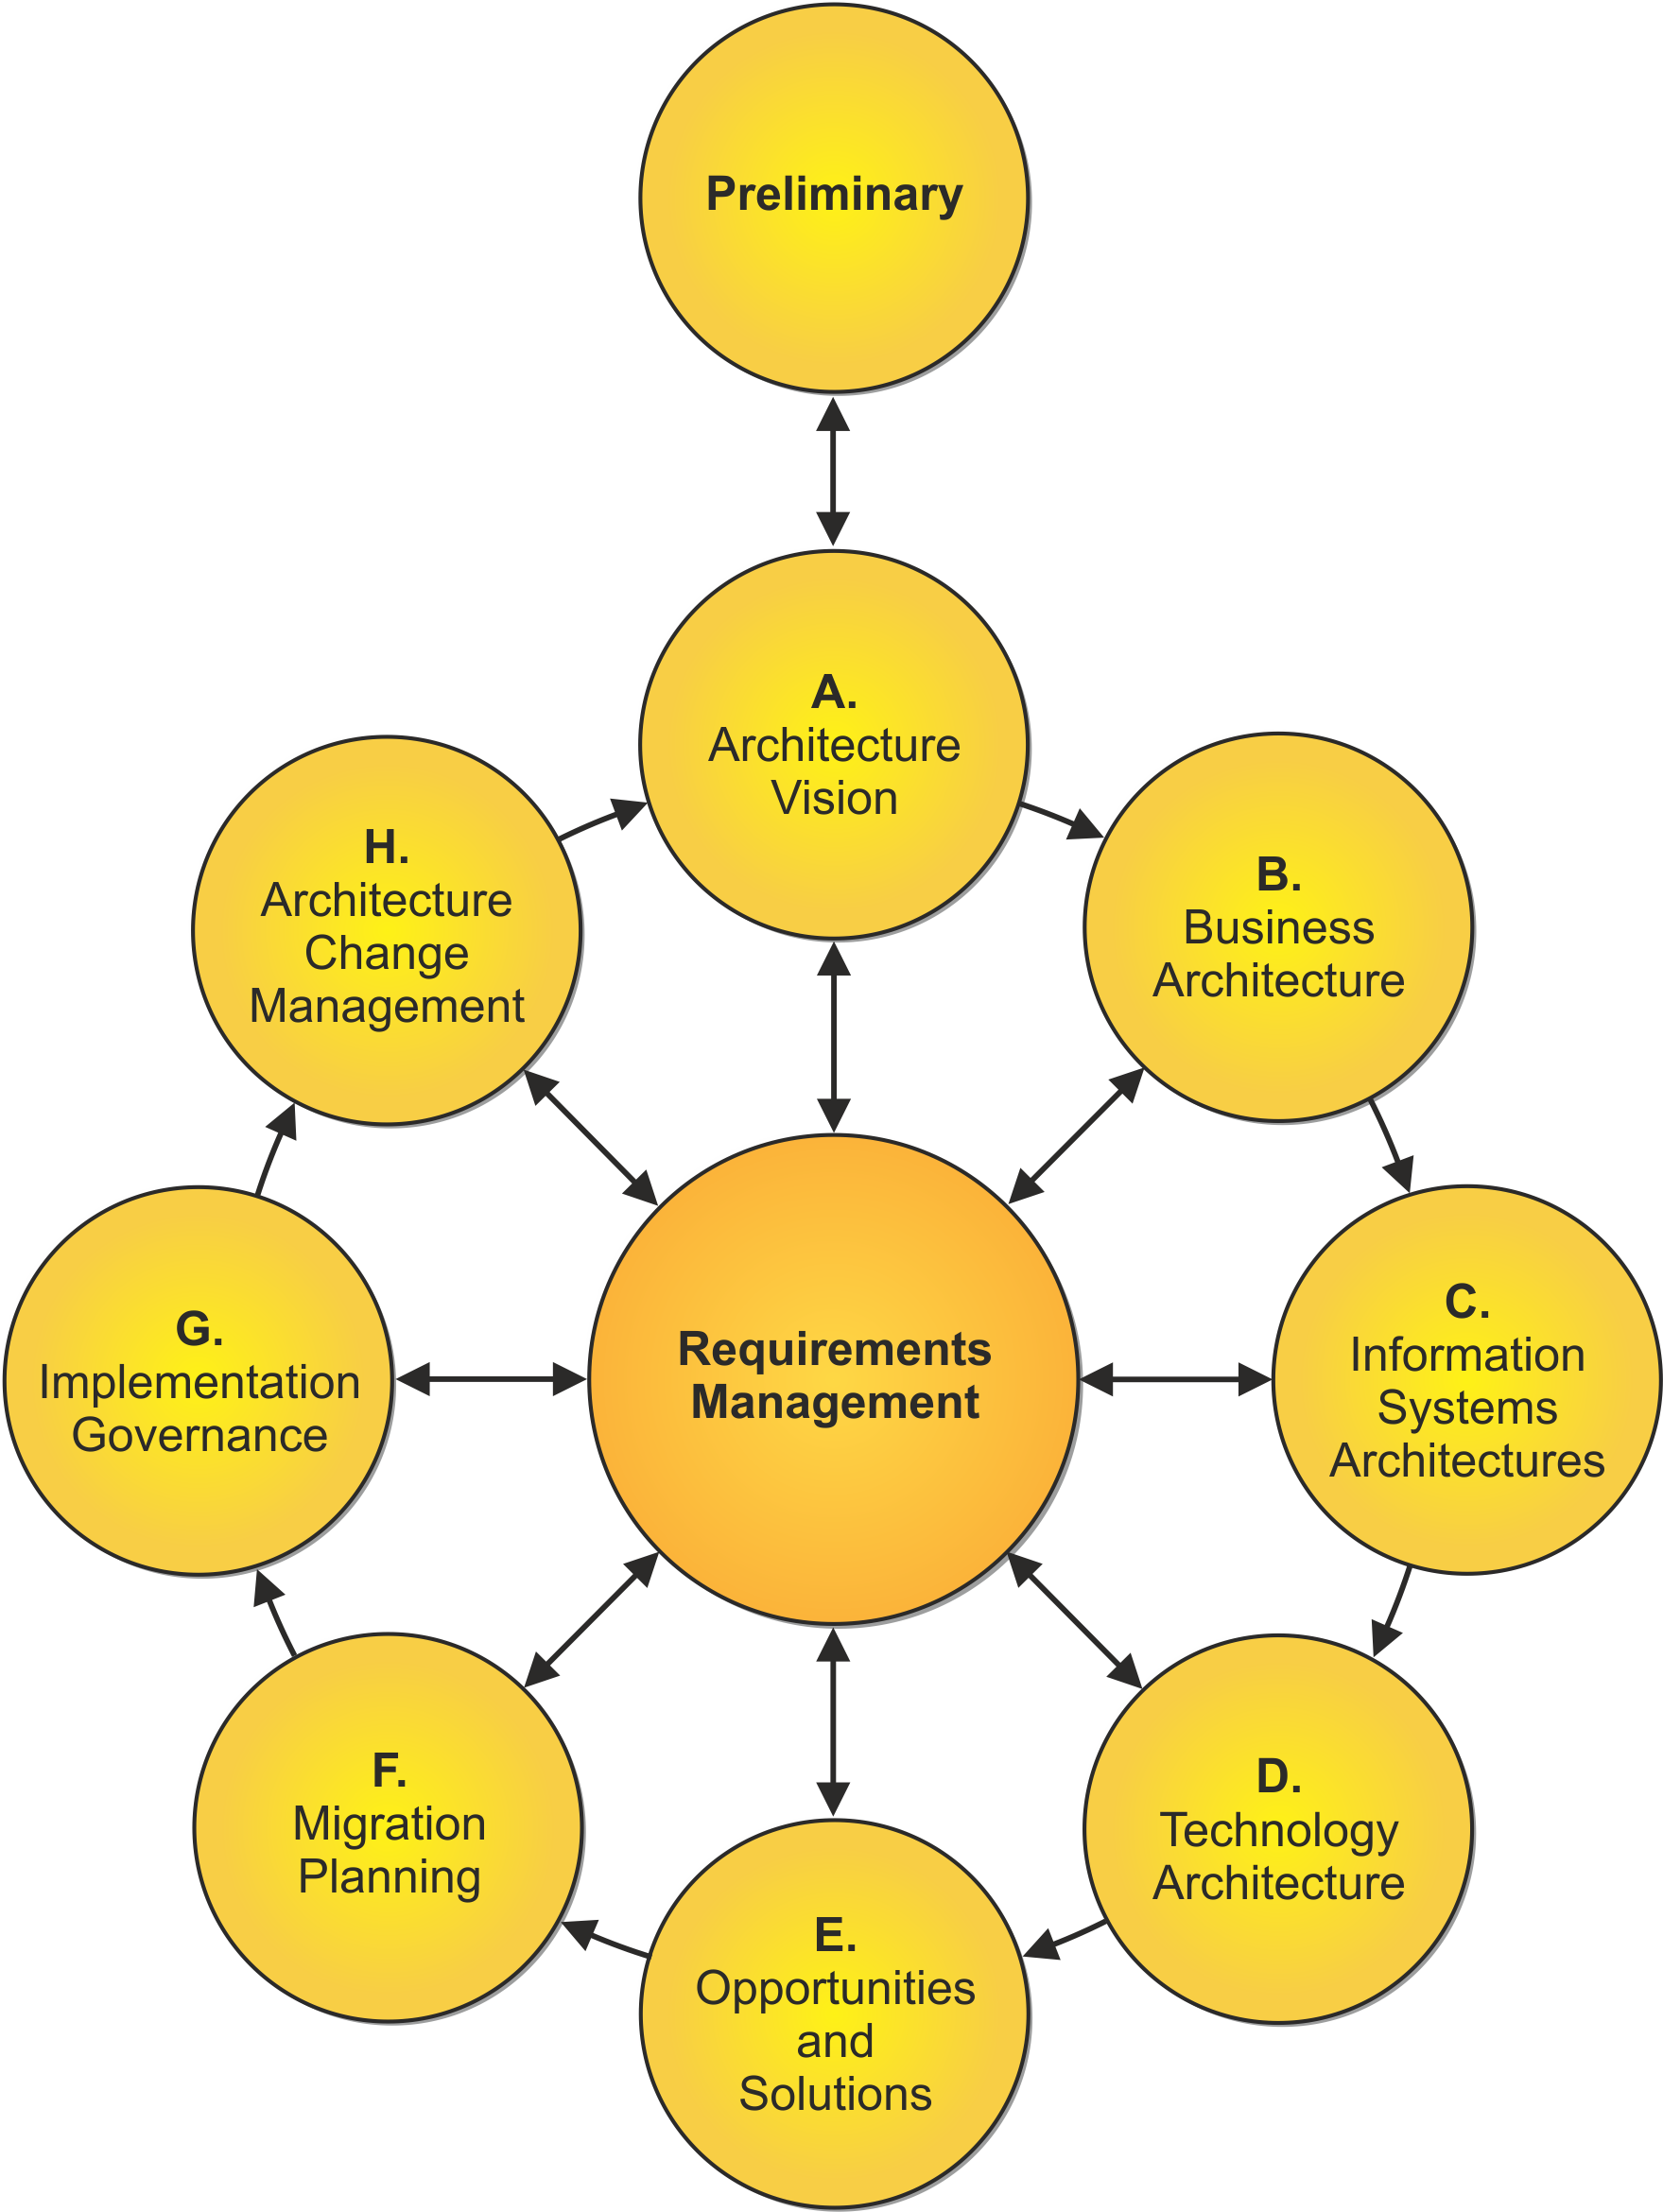
\includegraphics[scale=0.6]{img/togaf.png}
\decoRule
\caption{Example of an EAF structure (TOGAF).}
\label{fig:togaf}
\end{figure}

%-------------------------------------------

\subsection{Assets}
An \textbf{asset} is anything that represents a valuable resource for the enterprise. Protecting assets is the ultimate goal of security.

Assets usually fall into one of these categories:

\begin{itemize}
    \item \textbf{data} (typically the most valuable asset);
    \item \textbf{software components} (programs, applications, algorithms, etc.);
    \item \textbf{hardware components} (physical assets).
\end{itemize}

The security level of an asset derives from its properties; every asset has many, which can be set by the:

\begin{itemize}
    \item \textbf{law}: privacy laws, etc. (e.g. GDPR, National Security laws);
    \item \textbf{company}: whatever the company wants to do with its assets (e.g. guarantee to its users a certain level of privacy);
    \item \textbf{employer}: might be someone who needs extra security (e.g. the Department of Defense);
    \item \textbf{contract}: it could include Non Disclosure Agreements (NDAs) or other similar policies.
\end{itemize}

These properties, all of which are listed in the EAF, can either be \textbf{intrinsic} (imposed by an external entity, such as the law) or \textbf{extrinsic} (decided by the enterprise itself), and have to be specified in terms of \textbf{must}/\textbf{must not} (assets that 100\% have to comply to these properties) or \textbf{should}/\textbf{should not} (assets that must comply to these properties with at least a specified percentage).

All properties extend to all assets which handle other assets, e.g. if there is a requirement on the data, then all applications that handle it must comply to whatever requirements that data has. This means that security is as strong as the weakest link in the chain.

%----------------------------------------------------------------------------------------

\section{Risk management}
In general, we always need to have a plan in case something goes wrong. We do this by analyzing the working context in order to identify, evaluate and find countermeasures for all (or part of) possible risks:

\begin{enumerate}
    \item \textbf{risk identification};
    \item \textbf{risk evaluation};
    \item \textbf{implementation} of policies and countermeasures;
    \item \textbf{maintenance} of policies and countermeasures.
\end{enumerate}

Following these phases in order is mandatory, because points 3 and 4 are not possible without the first two.

%-------------------------------------------

\subsection{Risk assessment}
In order to evaluate risks we can use one of these two methodologies:

\begin{itemize}
    \item \textbf{qualitative risk assessment}: simple, clear and concise vision of risks;
    \item \textbf{quantitative risk assessment}: mathematical loss expectancy evaluation.
\end{itemize}

%----------------------

\subsubsection{Qualitative risk assessment}
Qualitative risk assessment uses a matrix to visually represent (in percentage) how much a risk is important. As seen in fig. \ref{fig:qualrisk}, the horizontal axis of the matrix indicates the risk's occurrence probability, while the vertical axis shows the risk's importance in terms of how much damage it would cause to the business (in either economical or reputational terms). This kind of evaluation offers a clear vision of what are the most serious risks, allowing us to identify those that should be patched as soon as possible.

\begin{figure}[H]
\centering
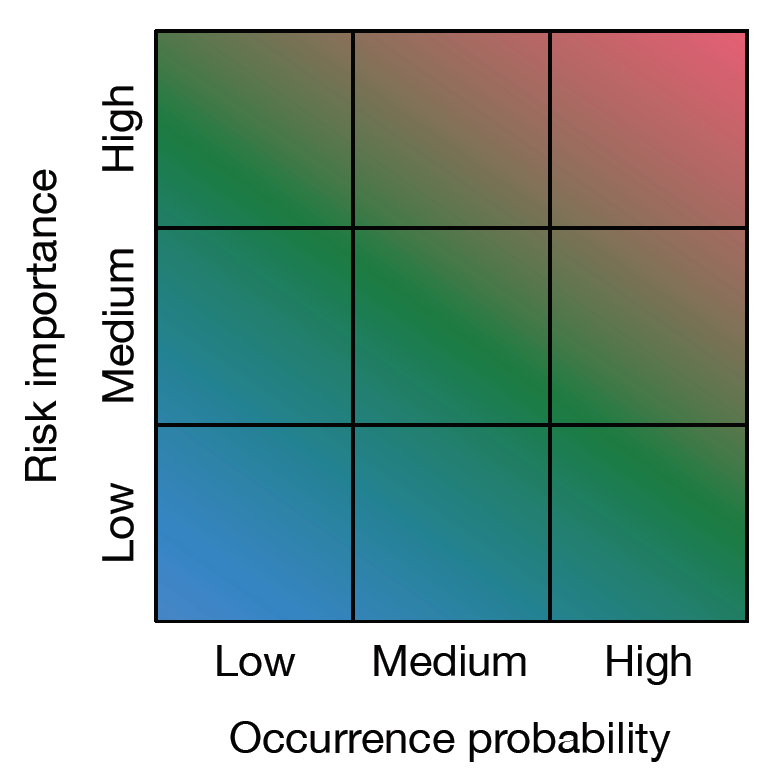
\includegraphics[scale=0.2]{img/qualitative_risk.png}
\decoRule
\caption{Qualitative risk assessment matrix.}
\label{fig:qualrisk}
\end{figure}

It must be noted, however, that not all risks should be covered; usually, risks in the central zone of the matrix (the one in green in fig. \ref{fig:qualrisk}) are considered acceptable, so they are acknowledged but nothing is done to avoid them.

Risks in the upper right area are mitigated in such a way that they can be moved to another zone: either towards the bottom to lower their occurrence probability, and/or the left, in order to lower their outcome (and possibly their cost, too); the exact direction depends on the cost and efficacy of the measures that need to be taken. This operation could be accomplished, for example, by transforming a primary asset into a secondary asset.

Generally, even though moving a risk directly to the lower left part of the matrix might seem ideal, doing this is not advised because the costs to achieve it would be too high, so it is usually better to deimplement some security measures and just keep the risks in the green area.

%----------------------

\subsubsection{Quantitative risk assessment}
Quantitative risk assessment is an analytical, less visual method that can be calculated using the following steps:

\begin{enumerate}
    \item \textbf{Asset Value (AV)} assignment: given an asset, we assign to it a certain economical value based on its importance;
    \item \textbf{Annual Rate of Occurrence (ARO) estimation}: as the name implies, we assess the number of times a certain risk is likely to occur in a year;
    \item \textbf{Exposure Factor (EF) estimation}: subjective, potential percentage of loss if a specific threat is realized;
    \item \textbf{Single-Loss Expectancy (SLE)}: $SLE = AV \cdot EF$; it represents the monetary value expected from the occurrence of a risk on an asset;
    \item \textbf{Annualized-Loss Expectancy (ALE)}: $ALE = SLE \cdot ARO$; as the formula implies, it is the product of the annual rate of occurrence (ARO) and the single loss expectancy (SLE).
\end{enumerate}

\emph{Beware of the average}: using it without knowing its probability distribution might be dangerous and counterproductive. It is usually safer and more informative to consider minimum and maximum values of a number.

%-------------------------------------------

\subsection{Risk analysis}

Correctly analyzing a risk requires many different phases and aspects to be taken in consideration, as illustrated in fig. \ref{fig:riskmodel}.

\begin{figure}[H]
\centering
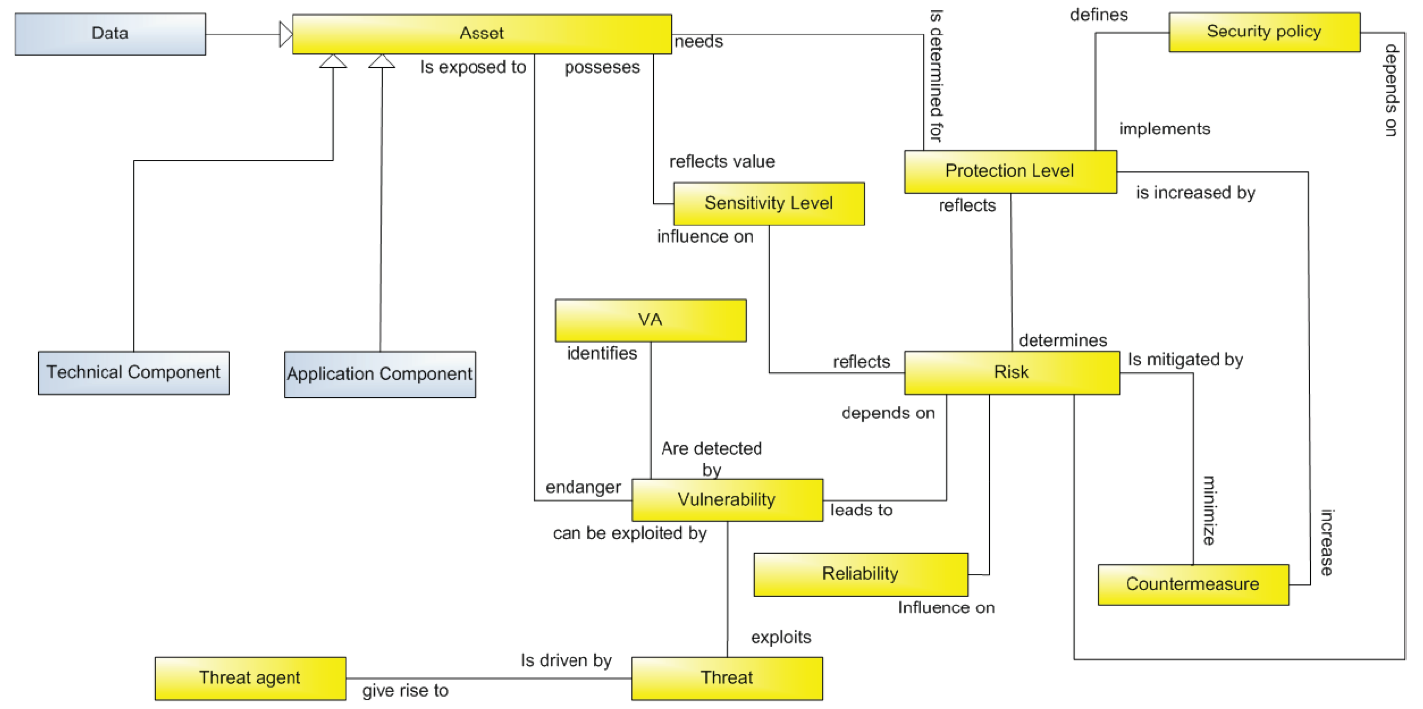
\includegraphics[scale=0.33]{img/risk_analysis.png}
\decoRule
\caption{A common risk analysis model.}
\label{fig:riskmodel}
\end{figure}

Given an \textbf{asset} and its \textbf{data}, the \textbf{sensitivity level} indicates how much the asset is important for the business; the higher this value, the higher the level of protection needed for the asset (and thus the lower the risk).

The \textbf{protection level} of an asset is directly correlated to its sensitivity level; it is implemented through:

\begin{enumerate}
    \item \textbf{security policies}: they mitigate the risk's occurrence (e.g. a database could implement an access control list, so that only authorized users could access it);
    \item \textbf{countermeasures}: they mitigate the risk's consequences \textit{after} its occurrence (e.g. a periodical system backup).
\end{enumerate}

A \textbf{risk} therefore depends on two large families of problems: \textbf{reliability}, which comprises all those factors that are determined by natural failures of the system, and \textbf{vulnerability}, the possibility that the system might be attacked by someone. Vulnerabilities are triggered by the existence of a bug in the protocols, components or the software used by the asset, namely in the:

\begin{itemize}
    \item \textbf{technical components} (hardware), usually subject to reliability problems;
    \item \textbf{application components} (software), usually subject to vulnerability problems.
\end{itemize}

Vulnerabilities can be found through the \textbf{Vulnerability Analysis} or \textbf{Vulnerability Assessment (VA)} process. It is a critical, open problem in software and network engineering, because even though some vulnerabilities are known and can be patched or at least partially covered, more often that not they are not known, so no countermeasures can be taken against them nor can they be taken into account when calculating risks. Thus, all vulnerabilities represent a serious \textbf{threat} that could be exploited by a \textbf{threat agent} - even though their existence only means that they have the potential to be abused of by a malicious agent, not that this will actually happen. In any case, a threat model can be used to better assess how a threat agent could damage an asset.

%----------------------------------------------------------------------------------------

\section{Threat model}
A \textbf{threat model} describes the capabilities that an attacker is assumed to be able to deploy against an asset. It should contain information about the resources available to the attacker, in terms of \textbf{available information}, \textbf{computing capability} (computational power depends on the attack) and \textbf{control of the system} (what the attacker would be able to do). The model also specifies the attacker's goals and how serious this person would be about his or her actions.

The threat model is necessary to define the risk probability, and it depends on the asset and the attacker's goals: the higher the goals, the greater the attacker's capabilities. Obviously, the model does not discuss physical threats only; many assets are immaterial, such as industrial secrets, and once they fall into the hands of an attacker they can be considered forever lost - even if the business still possesses them.

%-------------------------------------------

\subsection{Internet threat model}
\label{sec:internet_threat_model}
The generic Internet threat model (the one that is mostly used for devices connected to the Internet \textit{and} by people with a speck of brain) assumes these four points:

\begin{itemize}
    \item \textbf{Kerckhoff's principle}: the attacker knows everything about the system under attack. \textit{Security by obscurity}, an ideal which aims to make a system secure by intentionally hiding as many details about it as possible, should \textit{never} be pursued;
    \item the attacker has \textbf{enough computational power}: it might not always be limited to off-the-shelf\footnote{The definition of "off-the-shelf" actually depends on the level of the threat that we are talking about. An example: WiMax chipsets are nowhere to be found nowadays, because it is a dead standard; in order to get one to hack AeroMax communications at an airport, an attacker must either be a regular customer of AeroMax chipsets (which is extremely unlikely), or have a software defined radio and have developed the WiMax standard. Hacking AeroMax communications thus \textit{is} possible, but it actually costs too much for a single attacker to represent a real threat.} systems, as some attackers could also use highly specialized devices or tools, like AWS (Amazon Web Services);
    \item the attacker has \textbf{control of communication systems}: the attacker could inject data in the network. Note that the attacker might not be in full control the network, and/or could need to hide its presence, so it could either be able to only send data (active attacks, blind or almost blind) or to receive only (passive attacks);
    \item \textbf{does not} have control of the endpoints (these systems are protected).
\end{itemize}

In other words, even if the systems are not yet violated, the communication system might be
insecure. This assumption, however, can be relaxed in some cases.

%----------------------

\subsubsection{Attack examples}
\begin{itemize}

    \vspace{0.2em}
    
        \item \textbf{Passive attacks}
        \begin{itemize}
            \item Confidentiality violations
            \item Password stealing
            \item Offline cryptographic attacks
        \end{itemize}
        
    \vspace{0.2em}
        
    \item \textbf{Active attacks} (blind attacks)
        \begin{itemize}
            \item Replay attacks (a valid data transmission is maliciously or fraudulently repeated or delayed)
            \item Message insertion
            \item Message deletion
            \item Message modification
        \end{itemize}
\end{itemize}

These two kinds of attacks are very different in nature. A passive attacker usually has a very privileged position in the network, and his/her sending something in it would probably highlight his/her presence. For this reason, he/she usually just stays silent and only receives data.

%-------------------------------------------

\subsection{Network topology}
We cannot talk about threats without knowing the topology of the network we are working with, because it allows us to understand what an attacker is capable of as well as what he/she might desire to do, and how the network itself can be protected.

Depending on the topology, an attack can be classified as:

\begin{itemize}
    \item \textbf{on-path}: the attacker is on the \textit{natural} path of the data between the endpoints, either by sheer luck or thanks to his/her capabilities;
    \item \textbf{off-path}: the attacker does not see the data naturally flowing from a point A to another point B; in order to avoid being detected, he/she will have to pretend being B, but will not be able to see B's replies to A (blind attack);
    \item \textbf{link-local}: this is the worst case scenario, since the attacker is on the same link of the endpoint, in the same subnet or physically attached to the same switch/access point, a privileged position which permits a vast number of attacks.
\end{itemize}

We can assume that the attacker is off-path if and only if we control every single router and link between points A and B, and can be sure that the attacker has not violated any of these devices. Is this really feasible?

The answer to this question is that it depends on the geographical routing of the data, which in turn depends on the big communication links between the source and destination.

For example, there was once a project to lay a fiber optic cable between America and Asia, with one of the main exchange points in Hong Kong; the USA asked for this point to be removed, in order to avoid China's control, as they would have enabled on-path attacks. This request has not been satisfied, and thus the project has never been completed.

Note that mistakes in the routing tables that send data through places that should not be receiving them (e.g. San Francisco-Seattle through China) are at the order of the day, so in conclusion, never, ever assume that the attack is off-path, because an attacker can become on-path through a secondary attack to the routing.
\chapter{Introduction to cryptography} % Main chapter title
\label{ch:intro_crypto}

%----------------------------------------------------------------------------------------

\section{About security}
A stated in chapter \ref{chap:bc}, \textbf{information security} is not easy to define. Even the National Institute for Science and Technology (NIST, the main American institute for standards of connected systems) periodically changes its definition of security, showing how we switched from a computer-centric to an information-centric kind of security:

\begin{itemize}
    \item \textbf{Computer Security}: the protection afforded to an automated information system in order to attain the applicable objectives of preserving the integrity, availability and confidentiality of information system resources (includes hardware, software, firmware, information/data, and telecommunications)\footnote{NIST, October 1995, \url{https://doi.org/10.6028/NIST.SP.800-12}}.
    \item \textbf{Information Security}: the protection of information and information systems from unauthorized access, use, disclosure, disruption, modification, or destruction in order to ensure confidentiality, integrity, and availability\footnote{NIST, June 2017, \url{https://doi.org/10.6028/NIST.SP.800-12r1}}.
\end{itemize}

The ultimate goal thus is not to protect the computer, but the most important asset: data. The main aspects of security can be summarised in six concepts or policies, all of them strongly tied together: we cannot ensure confidentiality without authentication, integrity without access control, etc.:

\begin{enumerate}
    \item \textbf{access control};
    \item \textbf{authentication};
    \item \textbf{availability};
    \item \textbf{confidentiality};
    \item \textbf{integrity};
    \item \textbf{non repudiation}.
\end{enumerate}

In general, information security:
\begin{itemize}
    \item supports the mission of the organization;
    \item represents an integral element of sound management;
    \item implements protections so as to be commensurate with risk;
    \item makes roles and responsibilities explicit;
    \item pushes responsibilities for system owners beyond their own organization;
    \item requires a comprehensive and integrated approach;
    \item is assessed and monitored regularly;
    \item is constrained by societal and cultural factors.
\end{itemize}

%-------------------------------------------

\subsection{Access control}
\textbf{Access control} is the security technique that regulates who or what can view, use or access a place or other resources. It is strongly coupled with authentication, since it first assigns profiles to users, then limits service access to authorized profiles only. This technique consists of many rules that are not easy to define, and which require careful consideration. As one could imagine, to perform access control accounting techniques are used.

It is interesting noting that after a security violation, access control is the first policy to be examined. The network manager is the first person under investigation: he/she must prove that is not responsible for the attack, since it could have potentially serious legal consequences.

%-------------------------------------------

\subsection{Authentication}
\textbf{Authentication} is the process of verifying whether someone (or something) is, in fact, who (or what) it has declared to be: sometimes attackers might be posing as someone else in order to obtain reserved information meant for another person or device only.

Digital signature functions are used in order to obtain authentication.

%-------------------------------------------

\subsection{Availability}
\textbf{Availability} provides an assurance that the system and data (the overall service) can be accessed by and fulfill the requests of authorized users, whenever and wherever they are needed.

Service availability is the most difficult quality to guarantee, as it requires accurate network planning; for example, it is not achieved if a Denial of Service (DOS) attack is ongoing (in this case, our mission would be to make it so that realizing a DoS attack would be onerous for an attacker).

Note that periodically checking a system's availability is not an effective method for ensuring this policy, because an attacker could put the system down and bring it back up between two checks.

%-------------------------------------------

\subsection{Confidentiality}
\textbf{Confidentiality} is the security technique that protects information from being accessed by unauthorized parties. The exchanged data must remain \textbf{secret} between sender and receiver.

Normally, confidentiality is achieved by using cryptography algorithms, since networks allow for sniffing packets and non-encrypted data could potentially be read by someone else.

%-------------------------------------------

\subsection{Integrity}
\textbf{Integrity} is the assurance that the information is trustworthy and accurate. Data thus must reach destination without having been altered, either while being transmitted or stored. Usually data integrity is achieved by using hash functions.

Note that encrypted data does not ensure integrity, because sometimes cryptographic methods are vulnerable to attacks, and cryptographed data can be changed nonetheless (e.g. through a bit flipping attack). Also, there can be integrity without confidentiality.

%-------------------------------------------

\subsection{Non repudiation}
\textbf{Non repudiation} is the assurance that someone cannot deny the validity of something. It is a very important policy when documents are exchanged, and it is usually achieved with digital signature functions.

Digital signatures are a lot stronger than regular signatures\footnote{The human version of non repudiation, even though not very obvious, is quite funny. Consider signing a letter: even though we were the ones who signed it, we can always say that it was not our signature, and that someone else forged it. Nobody can claim that we are lying, because we ourselves are the ultimate authority that can say if a certain signature is ours and/or if we signed the letter. Only a graphological test (which, in fact, consists of another person analysing the signature - making all this rather paradoxical) could check if the signature has really been forged, but it is a long and painful process that is normally not undertaken.}. However, they are cryptographic methods, so they will be valid only for a number of years; after a certain deadline expires they are not valid anymore, meaning that anyone could claim anything about documents signed with an expired digital signature.

%----------------------------------------------------------------------------------------

\section{Cryptography principles}
\textbf{Cryptography} is the basis to do non repudiation (digital signatures), access control (because it is based on authentication, which in turn is based on digital signatures), integrity and confidentiality - basically everything but availability.

Cryptography is as old as the world; it means "to write something in an obscure way", and it describes how to exchange information in a way that only source and destination can understand.

In general, every message sent from a source to a destination contains information that can be quantified\footnote{If something contains information, then it cannot be random -  otherwise it would have no information.}. The point of cryptography is to hide this information to the point that an attacker cannot distinguish between meaningful data and random, uncorrelated noise (such as white noise). This is called \textbf{perfect secrecy}. Is it achievable? Yes, but actually no - and we are going to see why.

\vspace{0.2em}

\textbf{Note}: We must never invent our own cryptographic algorithm, because we will most certainly fail: it is a very hard mathematical task for which reinventing the wheel does not work (at all).

%-------------------------------------------

\subsection{Hash functions}
A \textbf{hash function} is a mathematical function that takes an input (in our case, a message) and outputs a \textbf{digest}, which is a \textit{smaller} piece of data of fixed dimension $n$ that has some mathematical properties (see fig. \ref{fig:hash}). Generally speaking, any minimal change to the input made by the hash function will provide a completely different result in the digest.

Hash functions are commonly used to resolve integrity guarantee of transmitted documents; they are realized with elementary operations such as \textbf{shift} and \textbf{XOR}, so they are computationally very fast.

\begin{figure}[H]
\centering
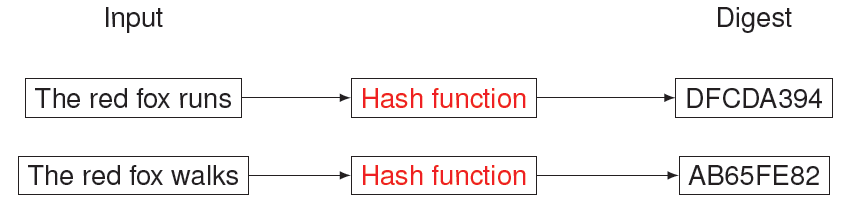
\includegraphics[scale=0.5]{img/hash.png}
\decoRule
\caption{An example of how hash functions work.}
\label{fig:hash}
\end{figure}

A hash function can and must be defined in terms of mathematical properties, because these are useful for a number of reasons. For example, if a person A (the sender) sends a message (some data) and its digest to another person B (the receiver), B can calculate the message's digest by using the same hash function as A (which is already known to both) and compare it with the one received from A, as shown in fig. \ref{fig:hashAB}. If the two digests are the same, then the message received from A has not been modified; otherwise, someone might have intentionally edited the data during transmission, and integrity has been lost.

\begin{figure}[H]
\centering
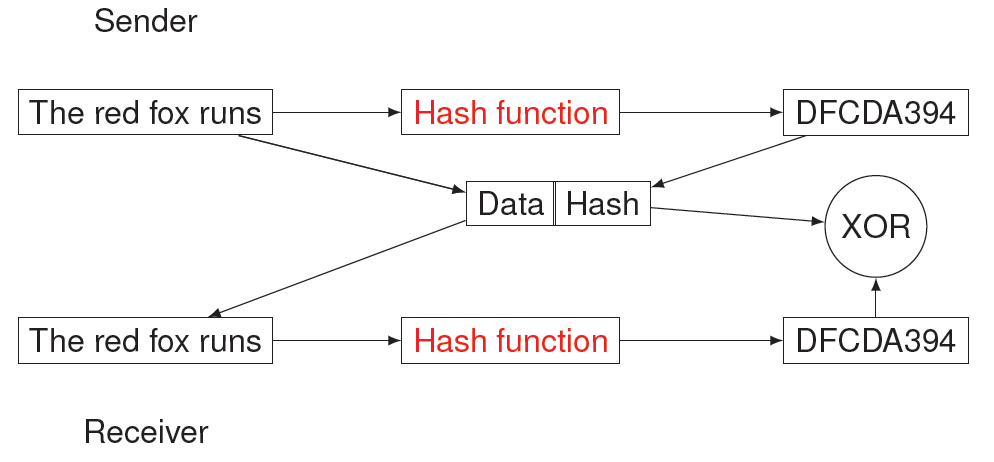
\includegraphics[scale=0.4]{img/hash_AB.png}
\decoRule
\caption{An example of how a digest can be useful to verify the integrity of a message. Note that, unlike this diagram, in real life we never want to send the message and its digest through the same channel, because an attacker could modify both and thus fool the receiver into thinking that the data has not been altered. Forcing an attacker to break two different channels represents an additional step in difficulty and security.}
\label{fig:hashAB}
\end{figure}

%----------------------

\subsubsection{Properties of hash functions}
In mathematical terms, a \textbf{hash function} is a function $H : X \rightarrow Y$ which maps an input $m$ of arbitrary finite length to an output $y = H(m)$ of fixed length $n$ (\textbf{ease of computation}). Domain $X$ contains all possibles messages, while codomain $Y$ all possibles digests; being $n$ of arbitrarily fixed length, $Y$ will be much smaller than $X$: $dim(X) \ll dim(Y)$ (\textbf{compression}).

Let us suppose that an attacker knows the digest of a message, but not the function that generated it. We should not be able to find another message that has the same hash - not because it is \textit{impossible}\footnote{\textbf{Impossible} means that a task cannot be performed, not even by brute force (i.e. trying every possible combination of bytes or secrets from a list, knowing the secret's length - an attack that is always possible).}, but because it is \textit{infeasible}\footnote{\textbf{Infeasible} means that a task cannot be performed within a reasonable amount of time with a reasonable amount of computational power.}. This property is called \textbf{pre-image resistance}, and it basically means that an attacker cannot pretend to be a legitimate user and send a message with a certain hash in order to later claim that the message was different (invalidating the original message).

\vspace{0.2em}

In short, the main properties of a hash function are:

\begin{enumerate}
    \item \textbf{compression}: $H : X \rightarrow Y$, with $dim(X) \ll dim(Y)$;
    \item \textbf{ease of computation}: given $H$ and an input $m$, $y = H(m)$ is very ease to compute;
    \item \textbf{pre-image resistance}: given a hash value $h$, it is computationally \textit{infeasible} to find any message $m$ such that $H(m) = h$;
    \item \textbf{2\textsuperscript{nd} pre-image resistance}: given a message $m$, it is computationally \textit{infeasible} to find any message $m'$ such that $H(m') = H(m)$;
    \item \textbf{collision resistance}: it is computationally infeasible to find any two distinct, arbitrarily chosen inputs $m$ and $m'$ such that $H(m') = H(m)$. This is the most difficult property to achieve in practice; note that having a hash function resistant to collision does not mean that it also has \textbf{pre-image resistance} and \textbf{2\textsuperscript{nd} pre-image resistance}.
\end{enumerate}

If a hash function does not respect even one of these properties, it cannot be used for cryptography purposes. However, not all of them are easy to achieve, nor can they be mathematically proven for an algorithm.

%-------------------------------------------

\subsection{HMAC}
We saw that hash functions are useful to guarantee integrity. What about authentication? For this task we need a \textbf{Hash Message Authentication Code}, or \textbf{HMAC}, which combines a hash function with a secret key.

The most used HMAC algorithm is the one from RFC 2104\footnote{\url{https://tools.ietf.org/pdf/rfc2104.pdf}}, which consists of the application of the hash function $H$ to a message $m$ and a shared secret key $K$ using equation \ref{eq:hmac} in order to obtain a digest in output:

\begin{equation}
\label{eq:hmac}
    \mathit{HMAC}(K,m) = H\Big((K' \oplus opad) \parallel H (K' \oplus ipad) \parallel m\Big)
\end{equation}
where

\begin{itemize}
    \item $H$ is a cryptographic hash function;
    \item $m$ is the message to be authenticated, divided into blocks of size $j$ (with $j$ depending on the hash function used);
    \item $K$ is the secret key;
    \item $K'$ is a block-sized key derived from the secret key $K$ either by padding to the right with zeros up to the block size, or by hashing down to less than or equal to the block size first and then padding to the right with zeros:
    
    \begin{equation}
        K' = \begin{cases}
        K &\text{if $dim(K) = j$}\\
        K \parallel pad(0) &\text{if $dim(K) < j$}\\
        H(K) &\text{if $dim(K) > j$}\\
        \end{cases}
    \end{equation}
    
    \item $\parallel$ denotes concatenation;
    \item $\oplus$ denotes bitwise exclusive-or (XOR);
    \item $opad$\footnote{\label{foot:pad}The values of $opad$ and $ipad$ are not critical to the security of the algorithm, but are defined in such a way to have a large Hamming distance from each other, and so the inner and outer keys will have fewer bits in common.} is the block-sized outer padding, consisting of bytes valued 0x5c repeated $\frac{j}{8}$ times;
    \item $ipad$\footref{foot:pad} is the block-sized inner padding, consisting of bytes valued 0x36 repeated $\frac{j}{8}$ times.
\end{itemize}

The secret key is first used to derive two keys – inner and outer; the first pass of the algorithm produces an internal hash derived from the message and the inner key, while the second pass produces the final HMAC code derived from the inner hash result and the outer key. 

It is worth noting that the final result will depend not only on the message, but also on the key, meaning that even if the attacker has the message he/she might not be able to decrypt it. $K$ should be large and random enough in order to not contain predictable bits, because otherwise an attacker could it find by using a brute force attack. If $K$ is shorter than $j$  bits we pad $K$ with a $0$ padding and then we either use it as it is, or we hash it and add a maximum entropy\footnote{\textbf{Entropy} is a measure of the informative content of a message. A message with maximum entropy is made entirely out of random bits (does not contain information).} number.

%----------------------

\subsubsection{HMAC in practice}
The digest can be calculated if and only if \textit{both} participants know the key $K$, so we will need authentication in order to ensure that they really are who they claim to be (and thus avoid giving the key to a potential attacker).

Suppose that A sends $m$ and $\mathit{HMAC}(K, m)$ to B in the same packet: if an attacker E intercepts both informations, he/she cannot recalculate $\mathit{HMAC}(K, m)$ because he/she does not know the key $K$, but he/she can easily modify $m$ in $m'$.

It is then clear that the main problems of HMAC are:

\begin{enumerate}
    \item finding a \textbf{secure way to exchange $K$} (and no, Internet is not the answer);
    \item \textbf{brute force attacks}: E could intercept a packet and try to predict $K$. This type of
attack is computationally infeasible, \textit{but} if the key is derived from a password, E can perform a dictionary
attack, since generating words in a dictionary takes only a few minutes. This issue is more common than one might think.
\end{enumerate}

%----------------------

\subsubsection{Final considerations}
HMAC does not state the hash function to be used, so we must choose the most appropriate one. We must be aware of the vulnerabilities that from time to time are found in hash functions and eventually change it, since the more they are used, the more they are studied and more vulnerabilities are found. For example, we should use \textbf{SHA3} instead of SHA2 or SHA1 (which are actually still widely used despite being severely broken).

If we use a weak hash function, an attacker could forge a message that would be considered by the receiver as valid; this is a very bad case, because the attacker could not just send false messages, but also find the secret key.

%-------------------------------------------

\subsection{Symmetric key encryption}
Symmetric key algorithms are algorithms for cryptography that use the same cryptographic keys for both encryption of plaintext (the original message) and decryption of ciphertext (the encoded message), as depicted in fig. \ref{fig:symm}. The keys, in practice, represent a shared secret between two or more parties that can be used to maintain a private information link.

Algorithms used for encryption and decryption can either be symmetrical or asymmetrical.

\begin{figure}[H]
\centering
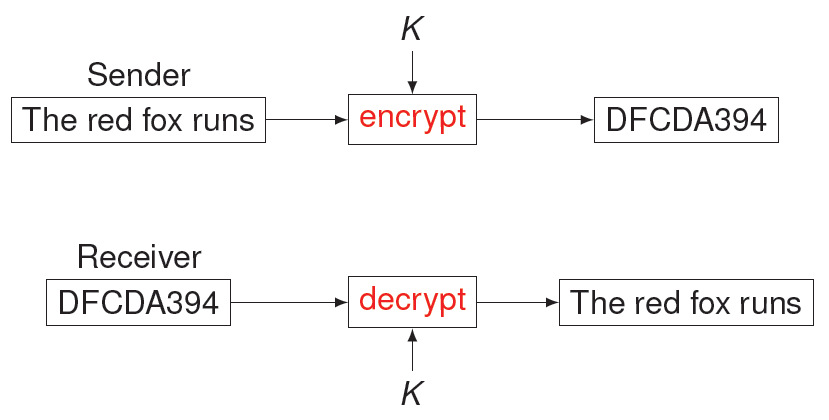
\includegraphics[scale=0.45]{img/symm.png}
\decoRule
\caption{Symmetric key encryption and decryption.}
\label{fig:symm}
\end{figure}

%----------------------

\subsubsection{Symmetric key encryption limitations}
The requirement that both parties have access to the secret key is one of the main drawbacks of symmetric key encryption, in comparison to public key encryption (also known as asymmetric key encryption).

Everything works if and only if we can ensure that nobody except for the sender and the receiver knows the keys. This statement is extremely weak: we can never assume it to be true, because the sender or the receiver could have been compromised, or the receiver is untrusted, and/or we cannot exchange different keys on the fly. In other words, symmetric key encryption is blind: it does not tell us anything about the identity of the sender, nor if the message has been modified or not.

%----------------------

\subsubsection{Use with HMAC}
In order to ensure the integrity of a message in symmetric key encryption, we can use it combined with HMAC in the following way:

\begin{enumerate}
    \item generate an HMAC with a secret key $K$;
    \item encrypt the whole message (HMAC included) with another secret key $K'$;
    \item by comparing the message and its HMAC, the receiver can tell if everything is right (or not).
\end{enumerate}

We use HMAC instead of a simple hash because if we used a hash and the attacker would recover the outer key $K'$ (the one used for symmetric encryption), he/she could change the message and its hash - so key $K'$ is an increased step in security.

Note that in spite of this method, the problems of privately sending the keys and ensuring the sender's identity remain.

%-------------------------------------------

\subsection{Asymmetric key encryption}
\textbf{Asymmetric key encryption} does not use a shared key; instead, both participants (which we name A and B) have two keys:

\begin{itemize}
    \item a \textbf{private key} $Pri_A$, $Pri_B$
    \item a \textbf{public key} $Pub_A$, $Pub_B$
\end{itemize}

Like their name implies, private keys must be kept secret: only A knows $Pri_A$ and only B knows $Pri_B$. Public keys can instead be disseminated anywhere, because they do not need to be protected; both A and B know $Pub_A$ and $Pub_B$, as well as possibly many other people. Obviously, for any person X, it must be computationally infeasible to obtain $Pri_X$ through $Pub_X$ and vice versa.

In an asymmetric key encryption scheme, anyone can encrypt messages using the public key, but only the holder of the paired private key can decrypt them.  An attacker could recover the message that has been sent, but because he/she does not know the private key, he/she will not be able to decrypt it. Thus, asymmetric key encryption works as follows (fig. \ref{fig:asymm}):

\begin{enumerate}
    \item sender (A) uses the receiver's (B) public key $Pub_B$ to encrypt his or her message $m$, obtaining $m'$;
    \item B uses his or her private key $Pri_B$ to decrypt $m'$.
\end{enumerate}

\begin{figure}[H]
\centering
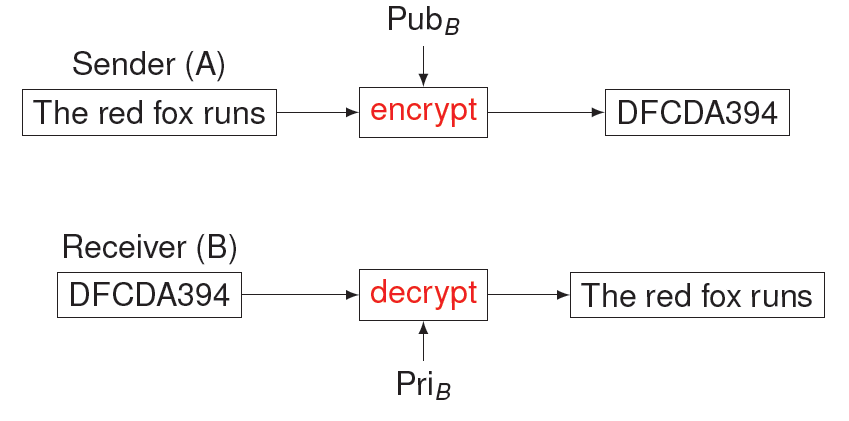
\includegraphics[scale=0.5]{img/asymmkey.png}
\decoRule
\caption{Asymmetric key encryption and decryption.}
\label{fig:asymm}
\end{figure}

The algorithm for encryption and decryption is the same for both operations: if we use the algorithm with one key we obtain a message that can be reverted to the original one by going through the algorithm with the second key (in other words, the second key decrypts the data encrypted by the first one).

Keys are usually joint generated with specific programs, like \textit{ssh-keygen} in Linux environments. It is not necessary to agree in advance on a common encryption/decryption key; an unpredictable (typically large and random) number is used to begin generation of an acceptable pair of keys suitable for use by an asymmetric key algorithm.

%----------------------

\subsubsection{Asymmetric key encryption: pros and cons}
The overall security of this method depends entirely on the \textbf{secrecy of the private key}: if we trust that the private key has been kept private by somebody or something, then whenever we get a message that can be decrypted by the public key paired with that specific private key, we know for sure that the only entity able to encrypt that message was the real sender. 

It is worth noting that in this way we guarantee \textbf{confidentiality}, and solve the problem of identity.

%-------------------------------------------

\subsection{Digital signature}
\textbf{Digital signature} is based on asymmetric key encryption, and in fact uses the same principles, only inverted: since in this case we do not care about confidentiality, but only want to \textbf{ensure the identity} (\textbf{non repudiation}) of the sender, we use A's private key $Pri_A$ to encrypt $m$. This way everybody will be able to decrypt the message with A's public key $Pub_A$, but we will guarantee that the sender was really A (the message has been \textbf{signed} by A, fig. \ref{fig:ds}).

\begin{figure}[H]
\centering
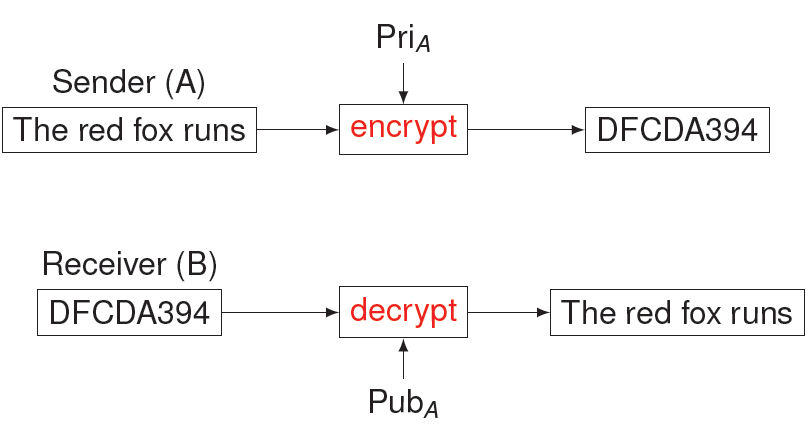
\includegraphics[scale=0.5]{img/ds.png}
\decoRule
\caption{Digital signature example.}
\label{fig:ds}
\end{figure}

%-------------------------------------------

\subsection{Mixed key encryption}
In day-to-day life neither purely symmetric nor purely asymmetric key encryption is used, but instead algorithms which combine these two methods in creative ways have been devised in order to obtain better security.

\begin{figure}[H]
\centering
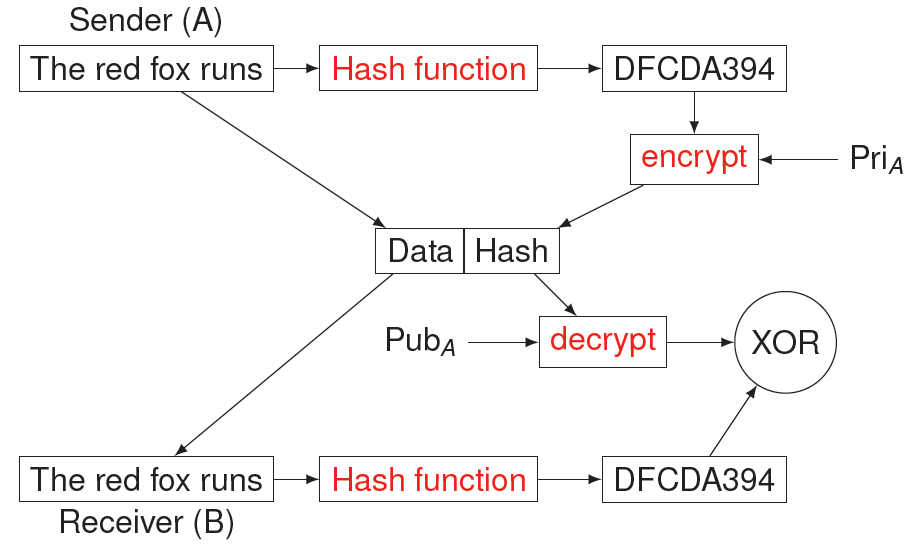
\includegraphics[scale=0.5]{img/mix.png}
\decoRule
\caption{An example of mixed symmetric and asymmetric key encryption.}
\label{fig:mix}
\end{figure}

The most common way of doing this is to encrypt a symmetric key with an asymmetric key. We use asymmetric cryptography to set up the communication, i.e. to negotiate a secret \textbf{session key} that is going to be used during that session. At this point the secret is known only by the sender and the receiver, and can be safely used to exchange private messages between them, ensuring confidentiality, integrity and identification.

Like its name implies, a session key is only valid during the communication session that it has been created for; new sessions will have to generate new secret keys.

%----------------------

\subsubsection{Multiple senders/receivers}
In cases like group chats where multiple ($n$) senders/receivers exist we must use a shared secret key in order to avoid computationally inefficient or even infeasible communication algorithms. However, this is a whole different problem which we do not discuss here; it is complicated by many additional factors, such as ensuring that someone banned out of the chatroom cannot return until not re-authenticated - while maintaining communication active for everyone else.
\chapter{Cryptography algorithms} % Main chapter title
\label{ch:crypto_algo}

%----------------------------------------------------------------------------------------

\section{Definitions}
We will begin this chapter by giving some useful definitions and theorems.

%-------------------------------------------

\subsection{Finite field (Galois field)}
A \textbf{finite field}, also called a \textbf{Galois field} and usually noted with $F_q$ or $GF(q)$, is a finite set of numbers on a field where multiplication, addition, subtraction and division (excluding division by zero) are defined and satisfy the rules of arithmetic known as the \textit{field axioms}:

\begin{itemize}
    \item associativity of addition and multiplication: $a + (b + c) = (a + b) + c$ and $a \cdot (b \cdot c) = (a \cdot b) \cdot c$;
        
    \item commutativity of addition and multiplication: $a + b = b + a$ and $a \cdot b = b \cdot a$;
    
    \item additive and multiplicative identity: there exist two different elements $0$ and $1$ in $F_q$ such that $a + 0 = a$ and $a \cdot 1 = a$;

    \item additive inverses: for every $a$ in $F_q$, there exists an element in $F_q$, denoted $-a$ and called the \textit{additive inverse} of $a$, such that $a + (-a) = 0$;
    
    \item multiplicative inverses: for every $a \neq 0$ in $F_q$, there exists an element in $F_q$, denoted by $a^{−1}$ or $\frac{1}{a}$ and called the \textit{multiplicative inverse} of $a$, such that $a \cdot a^{−1} = 1$;

    \item distributivity of multiplication over addition: $a \cdot (b+c) = (a \cdot b) + (a \cdot c)$
\end{itemize}

In this set of rules subtraction and division are the inverse operations of addition and multiplication, respectively. In general they are derived from them, but might not be defined as we know them, or it might be possible that they are not defined at all. Also, zero might not be the number zero, but a different element of the field; the same goes for one, the dot and plus: they are just operators. Basically, we have a field of objects that could be anything, and some operations defined on them.

%----------------------

\subsubsection{The Galois field $F_p$}
We can define Galois fields on a number of things; a common field, used in cryptography, is the \textbf{field of all positive numbers from $0$ to $p$}, where $p$ is a \textbf{prime number} or a product of prime numbers.

For each prime number $p$, the \textbf{prime field $F_p$ of order $p$} can be constructed as the integers $modulo\; p$\footnote{Given two positive numbers $a$ and $n$, $a\; modulo\; n$ (abbreviated as $a\; (mod\; n)$) is the remainder of the Euclidean division of $a$ by $n$, where $a$ is the dividend and $n$ is the divisor.}.

\vspace{0.5em}

\emph{Example} Using $p = 7$, a number in $F_7$ is $4$, which can be defined as $11\; (mod\; 7)$, $18\; (mod\; 7)$, etc.

Note that the \textbf{freshman's dream}, as the erroneous equation $(x+y)^n = x^n + y^n$ is sometimes called, is true in $F_p$ for powers of the prime number $p$, because in fields like this we have redefined all operations.

\vspace{0.5em}

\emph{Example} Using $p = 7$, we have:
\begin{center}
$(a + b)^7 = a^7 + 7a^6b + 21a^5b^2 + 35a^4b^3 + 35a^3b^4 + 21a^2b^5 + 7ab^6 + b^7$.
\end{center}

However, since $(7 \cdot x) (mod\; 7) = 0$ \; $\forall x \in F_7$, this means that:
\begin{center}
$(a + b)^7 (mod\; 7) = (a^7 + b^7) (mod\; 7)$.
\end{center}

This is possible because, having redefined all operations, $(a + b)^n (mod\; 7)$ can be rewritten in $F_p$ as:
\begin{center}
$\big((a + b) \cdot (a + b) \cdot ... \cdot (a + b)\big) (mod\; 7) = (a + b) (mod\; 7) \cdot (a + b) (mod\; 7) \cdot ... \cdot (a + b) (mod\; 7)$.
\end{center}

%-------------------------------------------

\subsection{Euler's totient function $\phi(n)$}
\textbf{Euler's totient function $\phi(n)$} counts the \textbf{relatively prime}\footnote{Two integers are \textbf{relatively prime} (or \textbf{coprime}) if there is no integer greater than one that divides them both (that is, their greatest common divisor is 1). Note that they do not have to be both prime (for example, the numbers 8 and 15 are coprime, but neither is prime).} positive integers up to a given integer $n$. In other words, it is the number of integers $k$ in the range $1 \leq k \leq n$ for which the greatest common divisor $gcd(n, k)$ is equal to 1, or how many relative primes exist that are smaller than $n$. The integers $k$ of this form are sometimes referred to as \textit{totatives} of $n$.

\vspace{0.5em}

\emph{Example} The totatives of $n = 9$ are the six numbers 1, 2, 4, 5, 7 and 8. They are all relatively prime to 9, but the other three numbers in this range, 3, 6, and 9 are not, since $gcd(9, 3) = gcd(9, 6) = 3$ and $gcd(9, 9) = 9$. Therefore, $\phi(9) = 6$.

\vspace{0.5em}

\emph{Example} $\phi(1) = 1$ since for $n = 1$ the only integer in the range from 1 to $n$ is 1 itself, and $gcd(1, 1) = 1$.

%----------------------

\subsubsection{Notable facts about $\phi(n)$}
\begin{itemize}
    \item If $p$ is a prime number and $k \geq 1$, then $\phi(p^k) = p^{k-1}(p - 1) = p^k(1 - \frac{1}{p})$.
    \item If $p$ and $q$ are coprime numbers, then $\phi(pq) = \phi(p)\phi(q)$.
    \item If $p$ and $q$ are \textit{both prime} numbers, then $\phi(pq) = (p-1)(q-1)$.
\end{itemize}

%----------------------

\subsubsection{Computing Euler's totient function}
There is no efficient way to calculate the totient function $\phi(x)$, even if we know that $x=pq$ and that $p$ and $q$ are prime numbers.

This happens because even in this case we still need to calculate the divisors of these numbers, and there is no (efficient) algorithm to find them; basically, all we can do is to try dividing our number for all numbers up to it (a brute force method).

Obviously, if we know that $x = pq$ \textit{and} either $p$ or $q$, we can easily find $\phi(x)$ - but this should never be the case in real life applications.

%----------------------

\subsection{Euler's theorem}
\textbf{Euler's theorem} (also known as the \textbf{Fermat–Euler theorem} or \textbf{Euler's totient theorem}) states that if $n$ and $a$ are coprime positive integers, then $a$ raised to the power of the totient of $n$ is equal to $1 (mod\; n)$, or:

\begin{equation}
    a^{\phi(n)} \equiv 1 (mod\; n)
\end{equation}

The definition of a Galois field tells us that the inverse of addition and multiplication \textit{exist}, but not \textit{how} they are defined. Usually they are defined in terms of regular addition and multiplication, but since this is not always possible (because in integer mathematics there is no division as we know it), we use this theorem to calculate the \textbf{multiplicative inverse}, which for a finite field such as a Galois field $F_{\phi(n)}$ is:

\begin{equation}
     a^{\phi(n)} = a \cdot  a^{\phi(n)-1} = a \cdot 1 (mod\; n) = a \;\;\;\;\;\;\;\;\;\; \forall a\neq 0
\end{equation}

%----------------------

\subsubsection{Chinese remainder theorem}
The \textbf{Chinese remainder theorem} states that if we know the remainders of the Euclidean division of an integer $n$ by several integers, then we can determine uniquely the remainder of the division of $n$ by the product of these integers, under the condition that the divisors are pairwise coprime.

We only mention this theorem, as we are not interested in its details. It is important, however, because together with Euler's totient theorem it is used in the \textbf{RSA cryptographic algorithm}.

%----------------------

\subsubsection{Trapdoor function}
A \textbf{trapdoor function} is an invertible function of which if we know its secret, then it is dramatically easy to solve; otherwise, it is next to impossible. In other words, we have the function but we do not know its inverse nor can we calculate it.

Clearly, a trapdoor function is desirable for making a good encryption algorithm, in order to make sure than encryption is easy while decryption is impossible or at least infeasible. This function should also be created using a solid mathematical approach (like definitions and theorems) in order to have proof that it is difficult to solve.

%----------------------------------------------------------------------------------------

\section{RSA algorithm}
The \textbf{RSA algorithm} (Rivest–Shamir–Adleman, from the names of the people who publicly described it in 1977) is a public-key cryptographic algorithm that is widely used for secure data transmission. RSA is a relatively slow algorithm, so it is not commonly used to directly encrypt user data. More often, RSA is used to transmit shared keys for symmetric key cryptography, which are then used for bulk encryption/decryption.

The security of RSA relies on the practical difficulty of factoring the product of two large prime numbers, the \textit{factoring problem}. Breaking RSA encryption is known as the \textit{RSA problem}; whether it is as difficult as the factoring problem is an open question. There are no published methods to defeat the system if a large enough key is used.

\newpage

Given:

\begin{itemize}
    \item $p$, $q$ prime numbers (\textit{private});
    \item $n = p \cdot q$ (\textit{public});
    \item $e$, $d$, coprime\footnote{To ensure that $e$ has a multiplicative inverse.} with $\phi(n)$ and multiplicative inverse $mod\; \phi(n)$, i.e. such that $e \cdot d = 1 (mod\; \phi(n)) = k \cdot \phi(n) + 1$ (\textit{private});
\end{itemize}

then, using Euler's totient function:

\begin{itemize}
    \item[] $m \equiv m^{\phi(n)+1}(mod\; n)$
    \item[] $m \equiv m^{k\cdot\phi(n)+1} (mod\; n) \;\;\;\;\; \forall k \in \mathbb{N}$
\end{itemize}

If we choose $e, d$ such that $d = \frac{k\cdot\phi(n)+1}{e}$, then we have:

\begin{itemize}
    \item[] $m \equiv m^{d \cdot e} (mod\; n)$
\end{itemize}

At this point, called $c = m^e (mod\; n)$ the cyphertext, we get:

\begin{itemize}
    \item[] $c^d (mod\; n) = m^{e^d} (mod\; n) = m^{e^{\frac{k\cdot\phi(n)+1}{e}}} (mod\; n) = m^{k\cdot\phi(n)+1} = m$
\end{itemize}

RSA is an interesting algorithm because even if an attacker knows $n$ and $e$, calculating any of the other numbers (either $\phi(n)$ or $d$) is computationally infeasible: although not impossible, it would take thousands of years even by using the best hardware available, due to the complexity of calculating a \textbf{discrete logarithm} and ultimately of \textbf{factorization}, which is a NP-complete problem.

Note, however, that between 1994 and 1996 a new algorithm was discovered, cutting the computational complexity of factorization by 20\%. Also, quantum computers could compute discrete logarithms in polynomial time.

%----------------------------------------------------------------------------------------

\section{Diffie-Hellman-Merkle algorithm}
The \textbf{Diffie–Hellman-Merkle} (DHM) key exchange is a method of securely exchanging cryptographic keys over a public (non-secure) channel, and was one of the first public-key protocols as conceived by Ralph Merkle, Whitfield Diffie and Martin Hellman.

Published in 1976 by Diffie and Hellman, this is the earliest publicly known work that proposed the idea of a private key and a corresponding public key; even though it is a little old, it is quite interesting and still debated. In 1997 it was revealed that James H. Ellis, Clifford Cocks, and Malcolm J. Williamson of GCHQ (\textit{Government Communications Headquarters}, British signals intelligence agency) had already shown in 1969 how public-key cryptography could be achieved. The question of paternity for this algorithm is largely academic, as the GCHQ paper has been ignored even by the GCHQ itself.

Given:

\begin{itemize}
    \item $p$ a very large prime number (\textit{public});
    \item $\alpha$ a primitive root\footnote{
        A \textbf{primitive root} is a number such that $\alpha (mod\; p)$ has multiplicative order $p-1$, or
            \begin{equation*}
                \alpha (mod\; p) \neq \alpha^2 (mod\; p) \neq \alpha^3 (mod\; p) \neq ... \neq \alpha^{p-1} (mod\; p)
            \end{equation*}
            \begin{equation}
                \alpha^i (mod\; p) \neq \alpha^j (mod\; p) \;\;\;\;\;\;\;\;\;\; \forall i,j \in [1, p-1]
            \end{equation}
        It can be demonstrated that there are $\phi(p-1)$ primitive roots for a prime number.
        }  (\textit{public});
\end{itemize}

the algorithm is as follows:

\begin{enumerate}
    \item A and B choose a secret number, $X_a$ and $X_b$ respectively;
    \item A sends to B $Y_a = \alpha^{X_a} (mod\; p)$;
    \item B sends to A $Y_b = \alpha^{X_b} (mod\; p)$;
    \item A computes $K_a = Y_{b}^{X_a} (mod\; p) = (\alpha^{X_b})^{X_a} (mod\; p)$;
    \item B computes $K_b = Y_{a}^{X_b} (mod\; p) = (\alpha^{X_a})^{X_b} (mod\; p)$;
\end{enumerate}

In the end, $K \equiv K_a \equiv K_b$ is the secret key that only A and B know. It is clear that DHM is similar to RSA, as they both make use of an exponential function of the type $c=m^e$ and need a logarithm (a discrete logarithm) as its inverse function.

This algorithm \textit{must} be paired with an identity verification mechanism, because an \textit{on-path} attacker could easily modify $Y_a$ and $Y_b$. We cannot crack DHM in linear time, unless we have a table of all primitive roots (since the only way to calculate a logarithm is to use tables or successive approximations) - which is is why we need $p$ very large: an inverse table for the logarithm function is possible to create, but if $p$ is large enough it would require too much space, making it infeasible.

%----------------------------------------------------------------------------------------

\section{One-time pad algorithm}
The \textbf{one-time pad} (OTP) is an encryption technique that cannot be cracked, but requires the use of a one-time pre-shared key the same size as, or longer than, the message being sent. In this technique, a plaintext $m$ is paired with a random secret key $k$ (also referred to as a one-time pad), then each bit or character of the plaintext is encrypted by combining it with the corresponding bit or character from the pad using modular addition (an invertible function): cyphertext will be $c=m\oplus k$, while decryption will be $m=c\oplus k$.

The resulting ciphertext will be impossible to decrypt or break if the following four conditions on the key $k$ are met:

\begin{enumerate}
    \item $k$ must be \textbf{truly random}\footnote{Every single bit has exactly a 50\% probability of being either $0$ or $1$.};
    \item $k$ must be at least \textbf{as long as the plaintext};
    \item $k$ must \textbf{never be reused} in whole or in part;
    \item $k$ must be kept \textbf{completely secret}.
\end{enumerate}

The one-time pad has a property termed \textbf{perfect secrecy}; that is, the ciphertext $c$ gives absolutely no additional information about the plaintext. This is because, given a truly random key that is used only once, a ciphertext can be translated into any plaintext of the same length, and all are equally likely. Thus, the a priori probability of a plaintext message $m$ is the same as the a posteriori probability of a plaintext message $m$ given the corresponding ciphertext.

%----------------------

\subsection*{OTP limitations}

The main problem with this algorithm is, of course, getting a perfectly random key $k$. Also, having a key that is as long as the message might be practically impossible.

A solution would be to generate the key with a pseudo-random number generator, and just
exchange the seed of the generator. This might look like a nice idea, but the pseudo-random number generator must really be generating random numbers - so in reality it does not actually work, because it will always have some kind of issue (like correlations between bits, or doubles, or triples, etc.) and, being \textit{pseudo}-random, it is an algorithm, meaning that if one knows the seed, he or she also knows the generated number. The better a pseudo-random generator is, the slower it executes; all of them, however, have at least a problem: their randomness depends entirely on the seeds, which must have certain properties in order to be effective.

%----------------------------------------------------------------------------------------

\section{Confusion and diffusion}
In cryptography, \textbf{confusion} and \textbf{diffusion} are two properties of the operation of a secure cipher identified by Claude Shannon in his 1945 classified report \textit{A Mathematical Theory of Cryptography}. These properties, when present, work to confuse the application of statistics and other methods of cryptanalysis.

These concepts are important in the design of robust hash functions and pseudo-random number generators, where \textbf{decorrelation} of the generated values is of paramount importance; basically, they should be enforced in algorithms in order to \textbf{prevent statistical cryptanalysis}.

These properties, however, are not mandatory for an algorithm to be safe. As an example, the one-time pad algorithm, which generates a ciphertext statistically independent of the plaintext, relies \textit{not} on either confusion, nor diffusion (this one because every bit of plaintext depends on a single bit of the key). This is true for all stream ciphers, because they are immune by definition to statistical cryptanalysis. Note that it might be argued that OTP does make use of confusion as the secret is not really the key $k$, which has the same length as $m$ and $c$, but the seed which generated it assuming that $k$ has been created using a pseudo-random number generator).

%----------------------

\subsection*{Confusion}
\textbf{Confusion} means that each binary digit (bit) of the ciphertext should depend on several parts of the key, obscuring the connections between the two. This property hides the relationship between the ciphertext and the key.

Confusion also makes it difficult to find the key from the ciphertext, and if a single bit in a key is changed, the calculation of the values of most or all of the bits in the ciphertext will be affected; it basically increases the \textbf{ambiguity} of ciphertext.

%----------------------

\subsection*{Diffusion}
\textbf{Diffusion} means that if we change a single bit of the plaintext, then (statistically) half of the bits in the ciphertext should change, and similarly, if we change one bit of the ciphertext, then approximately one half of the plaintext bits should change. Since a bit can have only two states, when they are all re-evaluated and changed from one seemingly random position to another, half of the bits will have changed state. In other words, the idea of diffusion is to \textbf{hide the relationship} between the ciphertext and the plain text.

%----------------------------------------------------------------------------------------

\section{Substitution algorithms}
\textbf{Substitution} algorithms are part of the so-called \textbf{Substitution-Permutation Networks} (SPNs), proposed by Shannon for the creation of robust and practical ciphers, such as the Feistel cipher. The one-time pad also is a special case of substitution algorithm.

Let us consider the case of block ciphers\footnote{A \textbf{block cipher} is a deterministic algorithm operating on fixed-length groups of bits, called \textit{blocks}.} on $n$ bits. In the most general case, for a fixed key $k$, such a cipher simply consists of an injective function $f$ from blocks of $n$ bits to blocks of $n$ bits or, in other words, a (static) map that changes the bits of a message:

\begin{equation*}
    f: \{ 0, 1\} \rightarrow \{ 0, 1\}^n
\end{equation*}

\emph{Example} Consider the following function for $n=2$ (2-bit map), where $f$ is a permutation of $\{0, 1\}^2.$:

\begin{center} % Centered list
$00 \rightarrow 01$\\
$01 \rightarrow 11$\\
$10 \rightarrow 00$\\
$11 \rightarrow 10$\\
\end{center}

\vspace{0.5em}

In the most general case, the number of possible transformations is equal to the possible permutations of the $2^n$ blocks, or $n^{n!}$. If we use small blocks, e.g. with $n=4$ or $n=5$, we get a classic monoalphabetic substitution cipher\footnote{In such a cipher, any character of plaintext from a given fixed set of characters is substituted by some other character from the same set.}.

Clearly, these ciphers are subscetible to \textbf{statistical cryptanalysis} attacks, because they do not have diffusion. In order to mitigate this risk we could use larger maps, but this is not feasible because the keys would have too many bits to be actually used in practice.

\vspace{0.5em}

\emph{Example} Given a 64-bit map ($n=64$), which is reasonably secure, the key would be represented by the permutation itself, which would be coded as $n\cdot 2^n = 64 \cdot 2^{64} \approx 10^{21}$. This is an impossible number of bits for a computer to handle.

%----------------------------------------------------------------------------------------

\section{Feistel cipher}
A \textbf{Feistel cipher} is a symmetric structure used in the construction of block ciphers, named after Horst Feistel who did pioneering research while working for IBM.

In a Feistel cipher, encryption and decryption are very similar operations, and both consist of iteratively running a function called a \textit{round function}\footnote{A \textbf{round function} is a function which takes two inputs, a data block and a subkey, and returns one output the same size as the data block.} a fixed number of times; the algorithm works as follows (also see fig. \ref{fig:feistel}):

\begin{enumerate}
    \item plaintext is divided in two parts $L_0$ and $R_0$, each of $w$ bits;
    \item $L_0$ and $R_0$ both go through $n$ rounds which have the same structure (plaintext is modified by a function $F$ which performs \textit{diffusion}) but use $n$ subkeys $K_1, ..., K_n$ generated from the main key $K$ such that $K_i \neq K_j \;\;\; \forall i, j \in [1, n], i \neq j$, and $K_i \neq K \;\;\; \forall \in [1, n]$;
    \item the two parts of plaintext exit the last round as $L_n$ and $R_n$ and go through a last step which swaps them (creating $L_{n+1}$ and $R_{n+1}$) to perform \textit{confusion}.
\end{enumerate}

The function $F$ is a cryptographically secure pseudo-random permutation function, where $K_i$ is the seed. This scheme is (more or less) used by all symmetric encryption algorithms.

An important advantage of Feistel ciphers is that the entire operation is guaranteed to be invertible (that is, encrypted data can be decrypted), even if the round function is not itself invertible. The round function can be thus made arbitrarily complicated, since it does not need to be designed to be invertible. Furthermore, the encryption and decryption operations are very similar, even identical in some cases; therefore, the size of the code or circuitry required to implement such a cipher is nearly halved: this cipher is easily translated into hardware.

\begin{figure}[H]
    \centering
    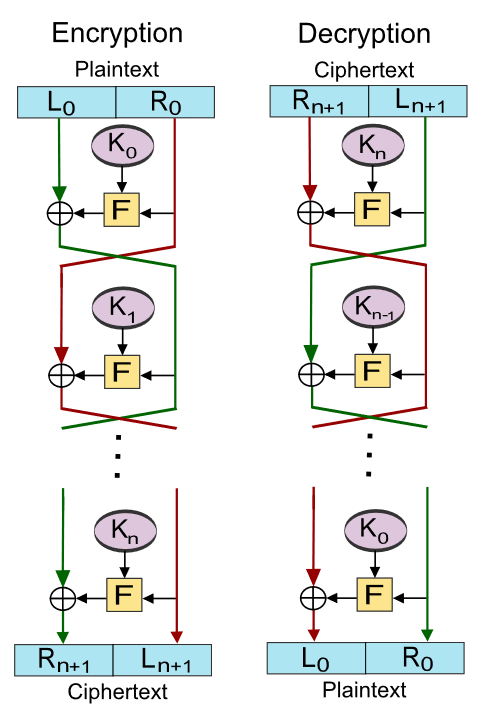
\includegraphics[scale=0.5]{img/feistel.png}
    \decoRule
    \caption{Feistel cipher encryption and decryption.}
    \label{fig:feistel}
\end{figure}

%----------------------------------------------------------------------------------------

\section{Elliptic curve cryptography}
\textbf{Elliptic curve cryptography} (ECC) is one of the most powerful but least understood types of cryptography in wide use today\footnote{Sullivan Nick, \textit{A (relatively easy to understand) primer on elliptic curve cryptography}, Ars Technica}. An increasing number of websites make extensive use of ECC to secure everything, from customers' HTTPS connections to how they pass data between data centers. It has fantastic pros and fantastic cons, but since we still do not know when and if there will be some way to invert it, we should not use it to encrypt very important stuff.

After the introduction of the RSA and Diffie-Hellman algorithms, researchers explored additional mathematics-based cryptographic solutions looking for other algorithms beyond factoring that would serve as good \textbf{trapdoor functions}. In 1985, cryptographic algorithms were proposed based on an esoteric branch of mathematics called \textit{elliptic curves}.

\begin{figure}[H]
    \centering
    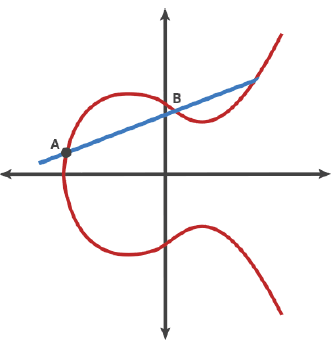
\includegraphics[scale=1]{img/elliptic.png}
    \decoRule
    \caption{An elliptic curve.}
    \label{fig:elliptic}
\end{figure}

An elliptic curve is a mathematical function of the form y$^2 = x^3 + ax + b$, as shown in fig. \ref{fig:elliptic}. It has two interesting properties:

\begin{itemize}
    \item it is symmetric with respect to the $x$-axis;
    \item any non-vertical line will intersect the curve in at most three places.
\end{itemize}

Let us imagine this curve as the setting for a bizarre game of billiards. Take any two points on the curve and draw a line through them; the line will intersect the curve at exactly one more place. In this game of billiards, we take a ball at point $A$ and shoot it toward point $B$. When it hits the curve, the ball bounces either straight up (if it is below the $x$-axis) or straight down (if it is above the $x$-axis) to the other side of the curve.

We can call this billiards move on two points a \textbf{dot function}. Any two points on a curve can be \textit{dotted} together to get a new point:

\begin{equation}
    A\; dot\; B = C
\end{equation}

We can also chain moves together to \textit{dot} a point with itself over and over:

\begin{center}
    $A\; dot\; A = B$ (this is the line tangent to the elliptic curve)\\
    $A\; dot\; B = C$ (also, $A\; dot\; B = B\; dot\; A$)\\
    $A\; dot\; C = D$
\end{center}

Basically, if we have two points and an initial point \textit{dotted} with itself $n$ times to arrive at a final point, finding out $n$ when we only know the final point and the first point is hard. To continue our bizarro billiards metaphor, imagine that one person plays our game alone in a room for a random period of time. It is easy for him or her to hit the ball over and over following the rules described above. If someone walks into the room later and sees where the ball has ended up, even if they know all the rules of the game and where the ball started, they cannot determine the number of times the ball was struck to get there without running through the whole game again until the ball gets to the same point. Easy to do, hard to undo: this is the basis for a very good trapdoor function.

Every couple of points $A$ and $B$ have a result $C$, because the elliptic curve is defined from a point called a \textbf{null point} and goes up to \textbf{infinity}, so on the $x$-axis from the null point (negative) to infinity (positive) we have every single $x$ covered.

Let us restrict ourselves to numbers in a fixed range like in RSA, meaning that rather than allowing any value for the points on the curve, we restrict ourselves to whole numbers in a fixed range. When computing the formula for the elliptic curve $y^2 = x^3 + ax + b$, we use the same trick of rolling over numbers when we hit the maximum. If we pick the maximum to be a prime number, the elliptic curve is called a \textbf{prime curve} and has excellent cryptographic properties.

\begin{figure}[H]
    \centering
    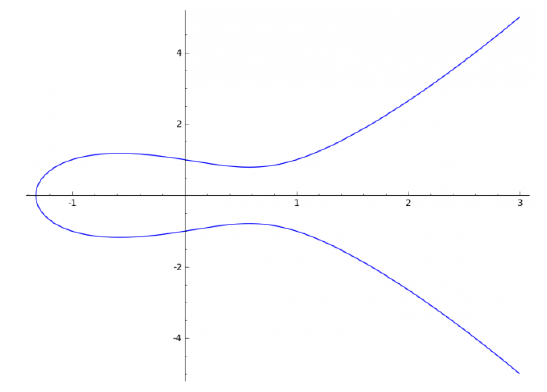
\includegraphics[scale=1]{img/elliptic2.png}
    \decoRule
    \caption{The curve $y^2 = x^3 - x + 1$ plotted for all numbers.}
    \label{fig:elliptic2}
\end{figure}

Figure \ref{fig:elliptic3} hardly looks like a curve in the traditional sense, but it is. It is like the original curve was wrapped around at the edges and only the parts of the curve that hit whole number coordinates are colored in, and we can even still see the horizontal symmetry.

In fact, we can still play the billiards game on this curve and dot points together. The equation for a line on the curve still has the same properties. Moreover, the dot operation can be efficiently computed: we can visualize the line between two points as a line that wraps around at the borders until it hits a point. It is like in our bizarro billiards game, when a ball hits the edge of the board (the max), then is magically transported to the opposite side of the table and continues on its path until reaching a point.

With this new curve representation, we can take messages and represent them as points on the curve. We could imagine taking a message and setting it as the $x$ coordinate and solving for $y$ to get a point on the curve. It is slightly more complicated than this in practice, but that is the general idea.

\begin{figure}[H]
    \centering
    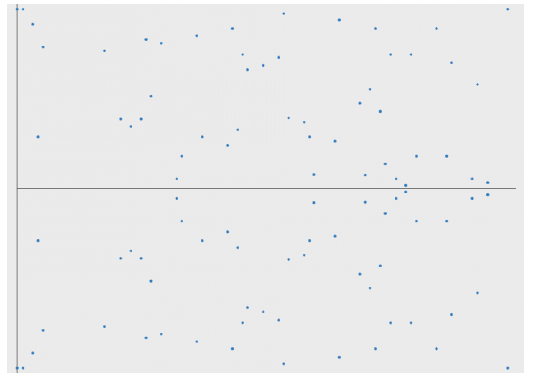
\includegraphics[scale=1]{img/elliptic3.png}
    \decoRule
    \caption{Plot of the same curve as \ref{fig:elliptic2} with only the whole number points represented, with a maximum of $97$.}
    \label{fig:elliptic3}
\end{figure}

An elliptic curve cryptosystem can be defined by picking a prime number as a maximum, a curve equation, and a public point on the curve. A private key is a number $priv$, and a public key is the public point \textit{dotted} with itself $priv$ times. Computing the private key from the public key in this kind of cryptosystem is called the \textbf{elliptic curve discrete logarithm function}. This turns out to be the trapdoor function we were looking for.

Basically, given a seed point $A$, we calculate $A\; dot\; A$ $n$ times: $A\; dot\; A$ will intersect another point $B$. If we do it again we will get another point, and so on. The thing is that if we know the starting point and how many times we elevated $A$ to itself (we did the dot function), calculating the endpoint is very easy, but if we only know the starting point and the endpoint, calculating how many times we did the dot function becomes dramatically harder (basically we will have to try doing it $n$ times).

%-------------------------------------------

\subsection*{Pros of elliptic functions}
The elliptic curve has been proposed by two mathematicians who were working for the NSA. It has been shown that is extremely hard to reverse-engineer, and that security is reached with less bytes in the key with respect to normal algorithms. Usually the shorter the key means the weaker is the algorithm; however, the elliptic curve was demonstrated that it is as strong as other algorithms with a shorter key, which is an extremely nice property: we can save bits and bytes in protocol exchanges and, depending on the algorithm, also be faster.

%-------------------------------------------

\subsection*{Cons of elliptic functions}
The problem that has been spotted almost immediately within the elliptic curve function was that there was no mathematical proof that the problem of inverting an elliptic curve was not treatable. We do not know if there is a way to invert the function; the inventors might have it but did not disclose it. Also, if we choose poorly $A$ and $B$ there might be a clever way to invert the algorithm.

In general, we must always make sure that the algorithms we use are top-notch; we must never use the new ones, which might not have been tested extensively and might suffer from unknown vulnerabilities, but instead we need the older, stronger ones, about which we know many properties.

%----------------------------------------------------------------------------------------

\section{Side-channel attacks}
A side-channel attack, also simply called a \textbf{side attack}, is any attack based on information gained from the \textit{implementation} of a computer system, rather than weaknesses in the implemented algorithm itself (e.g. cryptanalysis and software bugs).

General classes of side attacks include:

\begin{itemize}
    \item \textbf{timing attacks}: the attacker attempts to compromise a cryptosystem by analyzing the time taken to execute cryptographic algorithms. Since every logical operation in a computer takes time to execute, and the time can differ based on the input, with precise measurements of the time for each operation, an attacker can work backwards to the input;
    \item \textbf{heat and power monitoring attack}: the attacker studies the heat generation and/or power consumption of a cryptographic hardware device; by measuring these basic physical properties of a system, it is possible to learn a small amount of information about the data being manipulated;
    \item \textbf{random number generator attack}: the attacker subverts or exploits weaknesses within the process of random number generation. From a hardware point of view, this can be done by trying to either capture radio-frequency emissions from the computer (obtaining hard drive interrupt times from motor noise, for example), or to feed controlled signals into a supposedly random source (such as feeding a strong, known signal into a sound card).
\end{itemize}

In all cases, the underlying principle is that physical effects caused by the operation of a cryptosystem (on the side) can provide useful extra information about secrets in the system like, for example, the cryptographic key, partial state information, full or partial plaintexts and so forth.

The very basic point of all this is that we need to make sure that our algorithm performs either in the same way for any input, or in a random way for any input.
\chapter{Internet}
\label{ch:internet}

The \textbf{Internet} is a 60 years old project that still has legacy elements from its original implementation - an incredibly long time for a telecommunication network. It was built slowly, piece by piece, as it was initially developed for small, monolithic networks (that evolved based on what vendors wanted), and thus it was dramatically difficult to use.

Internet survived and thrived because of many factors, among which we can find:

\begin{itemize}
    \item \textbf{economical} factors: it was and still is (almost) free;
    \item \textbf{technological} factors: it was open, so anyone could devise their own protocols;
    \item \textbf{ease of use}: it was a lot  simpler than using raw sockets;
    \item \textbf{final users}: they were the same as the developers, so they could change whatever did not work as they wanted it to;
    \item \textbf{political} factors: telecommunications companies have driven all wireless and wired standards, even though they thought for a (too) long time that traditional communications (phone calls, SMS) were better.
\end{itemize}

The one thing that has always hindered (and probably always will) the Internet's development is the fact that it has to cope with everything that has already been rolled out (like the TCP/IP protocol), making it difficult to widespread new, better protocols.

%----------------------------------------------------------------------------------------

\section{History of Internet}
A detailed history of the Internet\footnote{Wikipedia, \textit{\url{http://en.wikipedia.org/wiki/Internet}}} and protocols like the one mentioned above\footnote{Wikipedia, \textit{\url{https://en.wikipedia.org/wiki/Internet\_protocol\_suite}}} can be easily found, well, on the Internet itself. It mostly consists of continuous attacks and attempts from companies and governments to make them their own, although fortunately nobody really succeeded.

Until the 70s, the Internet underwent a basic technical evolution, and vertical network models\footnote{\textbf{Vertical networks} connect people who have very specific interests. To be considered a vertical network, the focus of that group must be a specific niche.} were mostly used.

During the 80s and 90s the Internet became known to the world, and services began to be available to everyone. Competition between service providers started in those years.

Nowadays, the Internet is omnipresent and offers thousands of different services both legal or illegal; for this reason, it is often restricted by politics and economics. Net neutrality has become an important principle that many people advocate for.

%----------------------------------------------------------------------------------------

\section{What is the Internet made of?}
\label{sec:internetmadeof}
The Internet is not a single network, but an \textbf{interconnection of networks} and a collection of autonomous systems. It is based on \textbf{Request for Comments}, or \textbf{RFC}s, publications from the Internet Society (ISOC) and its associated bodies (like the Internet Engineering Task Force (IETF)), the main technical development and standards-setting bodies for the Internet. A RFC is authored by individuals or groups of engineers and computer scientists in the form of a memorandum describing methods, behaviors, research, or innovations applicable to the workings of the Internet and Internet-connected systems. It is submitted either for peer review or to convey new concepts, information, or occasional engineering humor.

Clearly, the physical host connections of the Internet are not as important as the protocols that make communication possible; although the Internet is based on TCP/IP, there are tons of other different protocols, and TCP/IP itself is very flexible (it can be applied in a lot of ways, including using actual birds\footnote{\label{foot:birds}\textbf{RFC 1149}, \textit{A Standard for the Transmission of IP Datagrams on Avian Carriers};\\\textbf{RFC 2549} \textit{IP over Avian Carriers with Quality of Service};\\ \textbf{RFC 6214} \textit{Adaptation of RFC 1149 for IPv6}.}).

%-------------------------------------------

\subsection{Internet mapping}

\begin{figure}[H]
  \centering
  \begin{minipage}[b]{0.4\textwidth}
    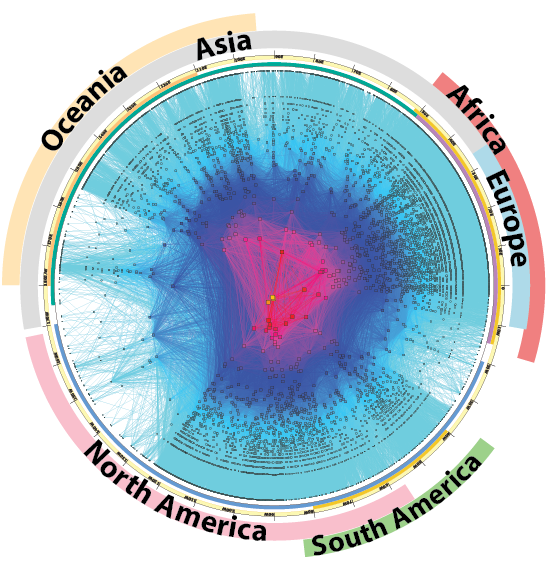
\includegraphics[scale=0.35]{img/caida2015.png}
    \decoRule
    \caption{CAIDA IPv4 2015 Internet map.}
    \label{fig:caida2015}
  \end{minipage}
  \hfill
  \begin{minipage}[b]{0.4\textwidth}
    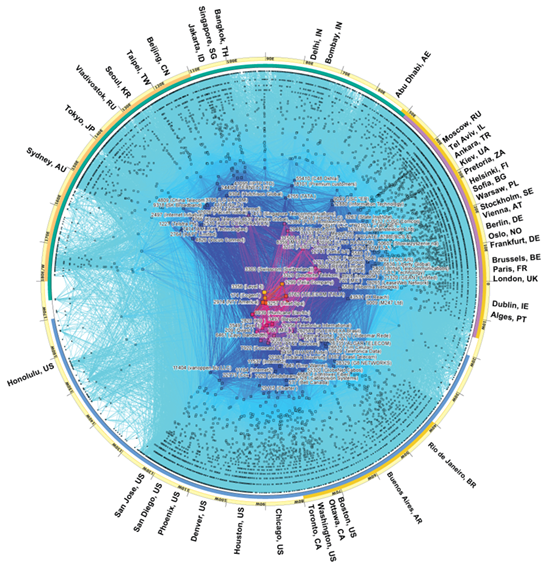
\includegraphics[scale=0.35]{img/caida2017.png}
    \decoRule
    \caption{CAIDA Ipv4 2017 Internet map.}
    \label{fig:caida2017}
  \end{minipage}
\end{figure}

Many organizations such as the Center for Applied Internet Data Analysis (\textbf{CAIDA}) perform \textbf{Internet mapping}, which is the study of the physical connectivity of the Internet. They collect, monitor, analyze, and visualize several forms of Internet traffic data concerning network topology, which is used for a variety of applications in business and society.

For example, in the CAIDA maps shown below (figures \ref{fig:caida2015} and \ref{fig:caida2017}), every dot is an autonomous system like a blob of routers, computers (thus not a single network node like a computer or a router), and is central or peripheral depending on how much traffic it generates or receives. Two dots are connected by a line if they exchange data directly, while red lines are Internet superhighways, which carry more traffic and are usually different from final users' lines.

%-------------------------------------------

\subsection{Some definitions}
Key principle: \textbf{K.I.S.S.}, \textit{Keep It Simple and Stupid}. Many things are hidden and/or simplified for our own safety.

%----------------------

\subsubsection*{Autonomous system}
Collection of connected Internet Protocol (IP) routing prefixes under the control of one or more network operators that presents a common, clearly defined routing policy to the Internet\footnote{RFC 1930, section 3.}. An AS is different from a subnet, as it is a management concept; any security policy at level of routing/network must be done into an autonomous system, and different autonomous systems will have different policies. There is no central authority that can tell an AS what policies to implement, because - like the name implies - they are autonomous.

%----------------------

\subsubsection*{Gateway}
Network entity also called the protocol converter. It can connect a computer of one network to another and defines the boundaries of a network; like a router, is an intermediate node which requires an IP interface for each subnet it is connected to. It resides in the third and/or seventh layer of the ISO/OSI protocol stack.

%----------------------

\subsubsection*{Host}
The source and destination of data, which must be uniquely identified by its IP address. It resides in the third layer of the ISO/OSI protocol stack.

%----------------------

\subsubsection*{Network}
Medium to which many nodes can be connected, on which every node has an address and which permits nodes connected to it to transfer messages to other nodes connected to it by merely providing the content of a message and the address of the destination node, then letting the network find the way to deliver the message to the destination node, possibly routing it through intermediate nodes.

%----------------------

\subsubsection*{Protocol stack}
Group of protocols that all work together to allow software or hardware to perform a function. In telecommunications, the TCP/IP protocol stack is a good example.

%----------------------

\subsubsection*{Router}
Network device that connects multiple networks together and controls the data traffic between them. A router is an intermediate node which needs an IP interface for each subnet it is connected to and, based on internal routing tables, it reads each incoming packet’s IP address and its destination IP address, then decides the shortest possible path to forward it after guessing the destination subnet (magic applies here):

\begin{itemize}
    \item if the destination is on a subnet directly connected to the router, it sends the packet directly;
    \item otherwise, finds the best next router and sends the packet to it.
\end{itemize}

Every router makes decisions on its own; this idea was developed in an attempt to make routers self-recovering. It resides in the third and/or seventh layer of the ISO/OSI protocol stack.

%----------------------

\subsubsection*{Routing table}
List of IP addresses that a router can connect to in order to transfer data.

%----------------------

\subsubsection*{Service Access Point (SAP)}
Identifying label for network endpoints used in ISO/OSI networking. Basically, the SAP is a conceptual location at which one ISO/OSI layer can request the services of another ISO/OSI layer.

%----------------------

\subsubsection*{Subnet}
Segment of a network identified by a \textit{\{Network Address\footnote{A \textbf{network address} is an identifier for a node or host on a telecommunications network.}, Subnet Mask}\} pair; it basically is a network inside a network. Through subnetting, network traffic can travel a shorter distance without passing through unnecessary routers to reach its destination, while routers are used to communicate between different subnets.

%----------------------

\subsubsection*{Subnet mask}
Similar to an IP address, but for only internal usage within a subnet. It is not indicated within data packets traversing the Internet, because those packets only indicate the destination IP address.

%----------------------------------------------------------------------------------------

\section{Structure of Internet}
How much should we know about Internet protocols? Nothing, and everything: a lot of security issues are strictly related to a protocol and how it works. In order to know or find vulnerabilities of a protocol we need to know it very well (not just because we studied it, but because we dissected it like a frog), even better than the person who devised it. However, we cannot ask anybody to know every single protocol that has ever been developed: the goal of this course is to teach what are the most important vulnerabilities, and a few things about how to find new ones. Mostly, in the end we should be able to know what to look for and where to get our hands dirty.

The idea behind the main Internet protocol stack model, the ISO/OSI model, is to divide the network in many separated layers, where the $n$-th layer offers services to the $(n+1)$-th layer and receives services from the $(n-1)$-th layer, each at their own SAP (fig. \ref{fig:layers_idea}). Note that if protocol $n$ communicates with a different layer on another device (one that is not an equivalent of layer $n$), then whoever devised it is either an idiot or a genius (most likely an idiot): this should \textit{never} happen.

\begin{figure}[H]
    \centering
    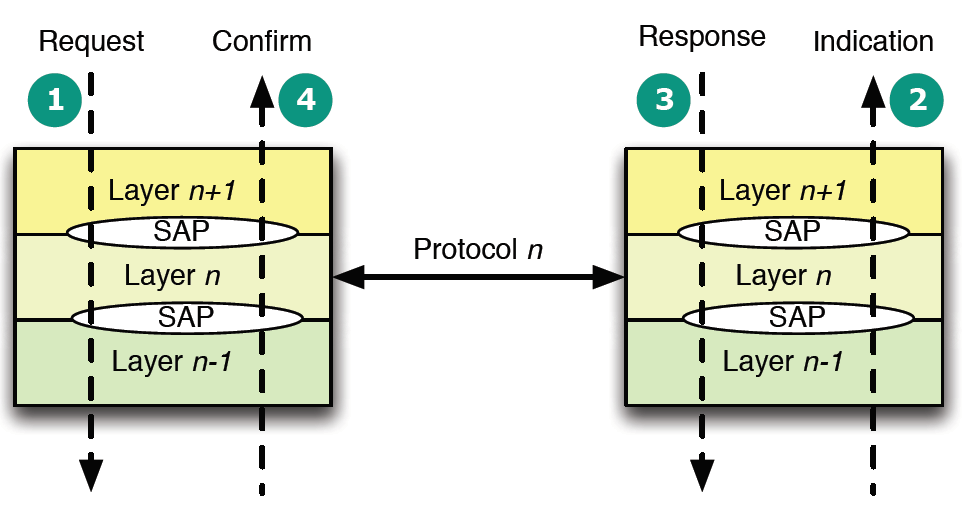
\includegraphics[scale=0.5]{img/layers_idea.png}
    \decoRule
    \caption{ISO/OSI model layer communication.}
    \label{fig:layers_idea}
\end{figure}

%----------------------

\subsubsection*{PDU and encapsulation}
In a network protocol made up of several layers each layer adds its own data in a header and (optionally) a trailer by building a \textbf{Protocol Data Unit} (PDU), as shown in figure \ref{fig:pdu}. The principle followed is that of \textbf{encapsulation}, a method of designing modular communication protocols in which logically separate functions in the network are abstracted from their underlying structures by inclusion or information hiding within higher level objects (see example in fig. \ref{fig:udp_pdu}).

Encapsulation is:

\begin{itemize}
    \item \textbf{recursive}: each layer adds its own header (and trailer, if any);
    \item \textbf{reversible}: it is always possible to correctly de-encapsulate the PDU of the layer above.
\end{itemize}

\begin{figure}[H]
    \centering
    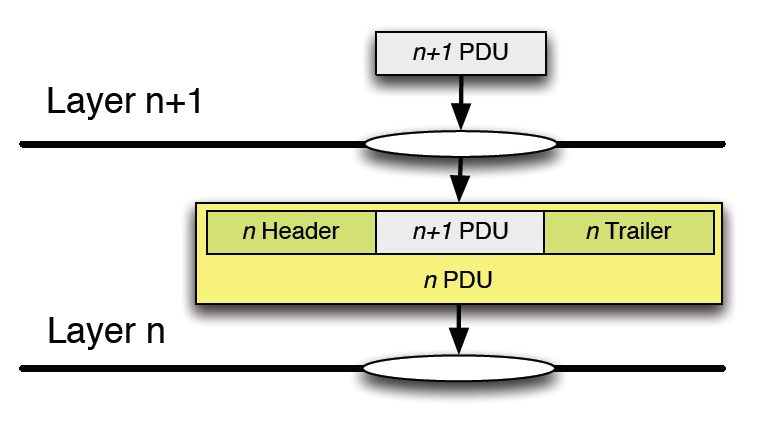
\includegraphics[scale=0.5]{img/pdu.png}
    \decoRule
    \caption{Protocol Data Unit (PDU) and encapsulation.}
    \label{fig:pdu}
\end{figure}

\begin{figure}[H]
    \centering
    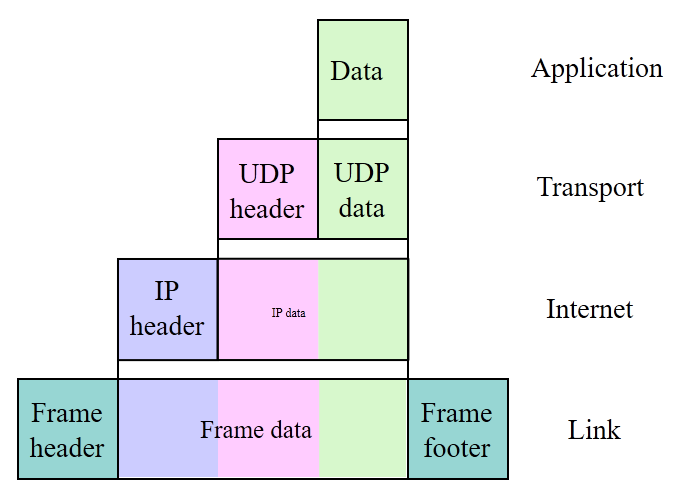
\includegraphics[scale=0.5]{img/udp_pdu.png}
    \decoRule
    \caption{An example of encapsulation of user data in the User Datagram Protocol (UDP) stack, in which each new layer includes the data from the previous layer, but without being able to identify which part of the data is the header or trailer from the previous layer. This effectively hides (encapsulates) the information from lower layers.}
    \label{fig:udp_pdu}
\end{figure}

\begin{figure}[H]
    \centering
    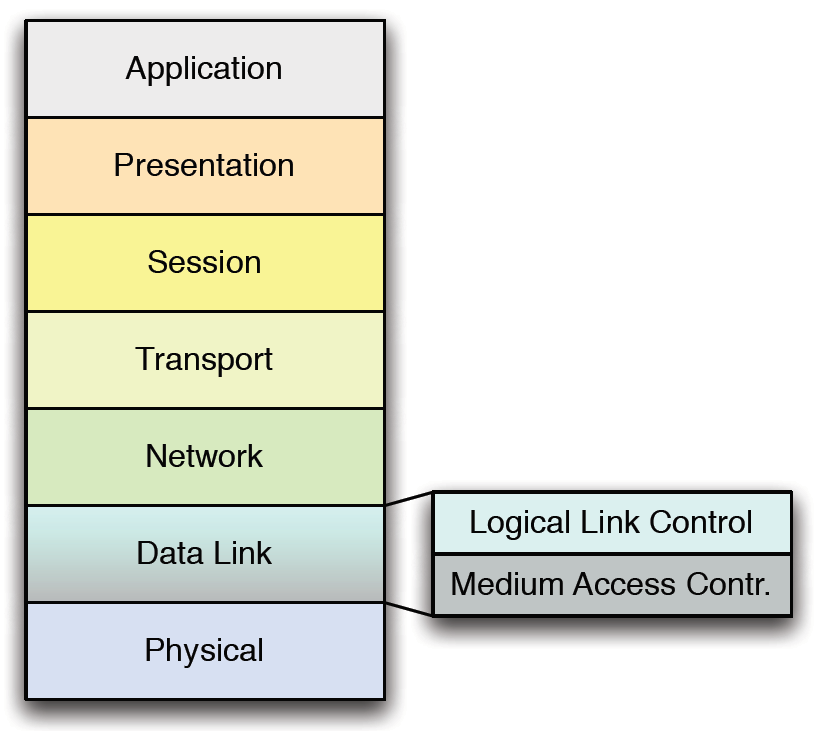
\includegraphics[scale=0.5]{img/isoosi.png}
    \decoRule
    \caption{ISO/OSI architecture.}
    \label{fig:isoosi}
\end{figure}

%-------------------------------------------

\subsection{ISO/OSI protocol stack}
\label{sec:iso_osi}
The \textbf{ISO\footnote{International Organization for Standardization.}/OSI\footnote{Open Systems Interconnection} model} is a conceptual model that characterises and standardises the communication functions of a telecommunication or computing system without regard to its underlying internal structure and technology. Its goal is the interoperability of diverse communication systems with standard communication protocols.

The ISO/OSI model has a seven layer architecture, meaning that it defines seven layers or levels in a complete communication system, as shown in figure \ref{fig:isoosi}. L1-L3 layers are also called \textbf{media layers}, as they are \textit{link-to-link}, while L4-L7 layers are the \textbf{host layers}, because they are end-to-end.

This model \textbf{forbids cross-layer communication} (services that are not tied to a given layer, but may affect more than one layer), even though it would have been useful. The two key principles of the model are:

\begin{itemize}
    \item \textbf{separation of concerns}: functionalities should not be duplicated;
    \item \textbf{information hiding}: implementation should remain hidden and separated from the interface.
\end{itemize}

It is not necessary to develop a separate layer for each and every function outlined in the model. However, by following the general guidelines it provides, developers are able to ensure that a certain level of compatibility is maintained.

%----------------------

\subsubsection*{1. Physical layer}
The \textbf{physical layer} is responsible for the transmission and reception of unstructured raw data between a device and a physical transmission medium. It converts the digital bits into electrical, radio, or optical signals.

%----------------------

\subsubsection*{2. Data Link layer}
The \textbf{data link layer} provides node-to-node data transfer — a link between two directly connected nodes. It detects and possibly corrects errors that may occur in the physical layer. It defines the protocol to establish and terminate a connection between two physically connected devices.

The IEEE 802 divides the data link layer into \textbf{two sublayers}:

\begin{itemize}
    \item \textbf{Medium access control layer} (MAC): responsible for controlling how devices in a network gain access to a medium and permission to transmit data;
    \item \textbf{Logical link control layer} (LLC): responsible for identifying and encapsulating network layer protocols; also controls error checking and frame synchronization.
\end{itemize}

%----------------------

\subsubsection*{3. Network layer}
The \textbf{network layer} provides the functional and procedural means of transferring packets from one node to another connected in different networks.

If the packet (message) is too large to be transmitted from one node to another on the data link layer between those nodes, the network may implement message delivery by splitting it into several fragments at one node, sending the fragments independently, and reassembling them at another node. It may, but does not need to, report delivery errors.

%----------------------

\subsubsection*{4. Transport layer}
The \textbf{transport layer} provides the functional and procedural means of transferring variable length data sequences from a source to a destination host, while maintaining the quality of service functions. It also controls the reliability of a given link through flow control\footnote{\textbf{Flow control} is the process of managing the rate of data transmission between two nodes to prevent a fast sender from overwhelming a slow receiver.}, segmentation/desegmentation, and error control. 

%----------------------

\subsubsection*{5. Session layer}
The \textbf{session layer} controls connections between computers. It establishes, manages (checkpoints, suspends and restarts) and (gracefully) terminates the connections between the local and remote applications.

%----------------------

\subsubsection*{6. Presentation layer}
The \textbf{presentation layer} establishes context between application-layer entities, in which the application-layer entities may use different syntax and semantics if the presentation service provides a mapping between them. If a mapping is available, presentation protocol data units are encapsulated into session protocol data units and passed down the protocol stack. This layer provides independence from data representation by translating between application and network formats. 

%----------------------

\subsubsection*{7. Application layer}
The \textbf{application layer} is the ISO/OSI layer closest to the end user, which means both the ISO/OSI application layer and the user interact directly with the software application. This layer interacts with software applications that implement a communicating component. Such application programs fall outside the scope of the ISO/OSI model. Application-layer functions typically include identifying communication partners, determining resource availability, and synchronizing communication.

%-------------------------------------------

\subsection{TCP/IP protocol stack}
The  \textbf{TCP/IP} stack is  the most commonly used protocol stack throughout the whole Internet. It violates the \textit{separation of concerns} principle of the ISO/OSI model (the truth is that other than being yet another communication stack, ISO/OSI and TCP/IP are two completely different protocols, like the sun and moon).

%----------------------

\subsubsection*{TCP}
Transmission Control Protocol is an Internet protocol suite which breaks up the message into TCP Segments and reassembling them at the receiving side.

%----------------------

\subsubsection*{IP}
An Internet Protocol address that is also known as an IP address is a numerical label. It is assigned to each device that is connected to a computer network which uses IP for communication. Its routing function allows internetworking and essentially establishes the Internet. Combination of IP with a TCP allows developing a virtual connection between a destination and a source.

\begin{figure}[H]
    \centering
    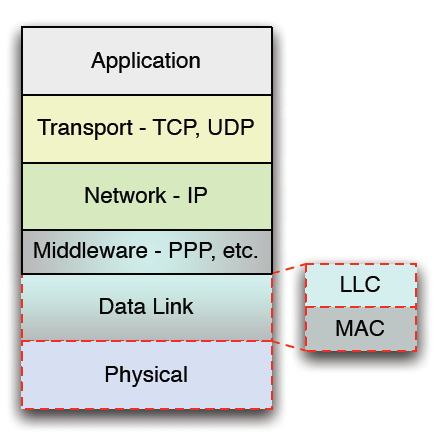
\includegraphics[scale=0.5]{img/tcp.png}
    \decoRule
    \caption{TCP/IP protocol stack architecture.}
    \label{fig:tcp}
\end{figure}

%----------------------

\subsubsection*{1. Data Link layer (L2)}
This layer routes the data between devices on the same network, and manages the exchange of data between the network and other devices. The TCP/IP stack only assumes that the underlying network will do its best to transfer packets from the
source to the destination; no further assumptions are made, so in reality we could use any data link layer (even birds like pigeons, as seen in section \ref{sec:internetmadeof}).

%----------------------

\subsubsection*{2. Network layer (L3)}
At this layer the Internet Protocol (IP) uses the IP address, consisting of a Network Identifier and a Host Identifier, to determine the address of the device it is communicating with.

%----------------------

\subsubsection*{3. Transport layer (L4)}
This is the part of the protocol stack where the Transport Control Protocol (TCP) can be found. TCP works by asking another device on the network if it is willing to accept information from the local device.

%----------------------

\subsubsection*{4. Application layer (L7)}
Protocols for specific functions such as e-mail (Simple Mail Transfer Protocol, SMTP) and file transfer (File Transfer Protocol, FTP) reside at this level.

%-------------------------------------------

\subsection{Addresses}
\textbf{Addresses} are important because, when used incorrectly, they can allow attackers to do lots of bad things: in order to pretend to be somebody else they need a sort of mask, and an address is the best mask behind which an attacker can hide.

%----------------------

\subsubsection{MAC address}
A \textbf{Media Access Control} (\textbf{MAC}) \textbf{address} (also wrongly called \textit{physical address}) is usually a fixed address which has a format (a length) dependent on the technology used by the device's network card.

\vspace{0.5em}

\emph{Example} Ethernet and WiFi devices both have 48-bit MAC addresses; IEEE 802.15.4 has 48-bit or 64-bit MAC address; LTE and other wireless interfaces have different length addresses, and they usually have a particular meaning.

\vspace{0.5em}

The only real requirement for MAC addresses is not that they are unique in the whole Internet, but that there cannot be two different network cards with the same MAC address in the same local network, since the MAC identifies a network card in that specific network.

It is important to note that a card can have more than one MAC address; it depends on the hardware. Usually, most network cards do not allow us to do this, because with more MAC addresses we would be seen in the network as more devices, even though we only have one. Also, there exist hardware devices which can be programmed to filter packets based on more than one MAC address: technically, everything is possible.

Notably, in a network there are also special MAC addresses, like the broadcast address (which directs packets to every network card able to receive it).

By default, when a NIC (network interface controller, another name for what is usually a network card) receives a packet, it checks its header and drops it unless it is addressed to that NIC's MAC address or is a broadcast or multicast addressed packet. In \textbf{promiscuous mode} (a special mode available to all NICs) however, the NIC allows all packets through, thus allowing the computer to read and reply to packets intended for other machines or network devices.

Promiscuous mode can be used in a malicious way to capture private data in transit on a network, so we might be interested in detecting network devices that are in promiscuous mode in order to find potential attackers.

The role of the MAC address is not to prevent this mode; it has been devised for efficiency only: the bus between the NIC and the CPU is a bottleneck, so a network card which is not in promiscuous mode filters all received packets based on their headers and MAC addresses in order to avoid slowing down traffic on the bus with useless packets.

%----------------------

\subsubsection{Numerical address}
\textit{\textbf{Numerical address}} is just another name for \textbf{IP address}, which is necessary for the routing process. It must be compliant with the network we are attached to (meaning that it must be in the range of addresses managed by the router on that network), and it is usually assigned by a network manager. An IP address serves two main functions: \textbf{host identification} and \textbf{location addressing}, and for this reason it must be \textbf{unique} in the global network.

\vspace{0.5em}

\emph{Example} 150.217.8.24 is an IPv4 address, a type of numerical address at layer 3 written in its canonical form.

\vspace{0.5em}

Note that in reality all addresses are binary numbers of a fixed length (32 bits for IPv4 and 128 bits for IPv6). Also, it is possible and perfectly legit for a device to have more than one IP address, for various reasons (for example, if the host is connected to more than one network).

%----------------------

\subsubsection{Alphanumeric address}
Alphanumeric addresses are special addresses that correspond to IP addresses. They are completely free, and their only requirement is that somebody (the DNS) maps them directly and reversely to an IP address, based on a database.

\vspace{0.5em}

\emph{Example} \textit{daconets.dinfo.unifi.it} is an alphanumeric address.

\vspace{0.5em}

In general, a host can have one of more MAC addresses on the same network card, one of more IP addresses for each MAC address, and each IP address can have none, one or more alphanumeric addresses, while on the other hand an alphanumeric address can be mapped to one or more IP addresses (because it consists of a database). However, having one IP mapped to more than one MAC address is not recommended, as lots of bad things can happen. The only case when is a good idea to have this solution is either when being an expert network engineer who attached the device to two different networks, or assigning our IP address to two NICs, one of which is silent.

If an alphanumeric address is mapped to more than one IP address, then it is a responsibility of the source host to choose which one is better, based on either randomness or speed.

%-------------------------------------------

\subsection{IPv4 addressing}
Historically (1980s), IPv4 divided its $2^{32}$ addresses into five different blocks, or \textit{classes}, each for different purposes. The IP address was divided in three parts, the $netID$, $subnetID$ and $hostID$ (see fig. \ref{fig:ipv4classes}), with the $netID$ dependent on the network's class. It was soon observed that this architecture was too complicated and inefficient (routing tables would have been too long), so they were replaced in 1993 by the \textbf{Classless Inter-Domain Routing} (\textbf{CIDR}).

CIDR notation, which takes the form $x.x.x.x/y$ and eliminates the distinction between $netID$ and $subnetID$, is constructed from an IP address, a slash ('/') character, and a decimal number. The trailing number is the count of leading 1-bits (those relevant for the routing process) in the subnet mask. This notation allows the \textit{joining} of addresses differing for their least significant bit. Note that the number of bits of a mask is not necessarily a multiple of a byte (this actually complicates things if we are looking at the address in its canonical form).

If we want to check if two address are in the same subnet (equivalently, if they can be reached directly through the MAC address), then we check if their network parts (those which are specified by the number of bits in the mask) are identical.

\vspace{0.5em}

\emph{Example} The addresses 150.217.8.0/24 and 150.217.9.0/24 differ only for their Least Significant Bit (LSB), so they are joined to form the address 150.217.8.0/23.

\vspace{0.5em}

\emph{Example} 192.168.100.14/24 represents the IPv4 address 192.168.100.14 and its associated routing prefix 192.168.100.0 or, equivalently, its subnet mask 255.255.255.0, which has 24 leading 1-bits.

A 32-bit mask identifies a single host and would have a subnet mask equal to 255.255.255.255, while 24-bit or less masks, like 255.255.255.0, identify networks: the block 192.168.100.0/22 represents the 1024 IPv4 addresses from 192.168.100.0 to 192.168.103.255.

\begin{figure}[H]
    \centering
    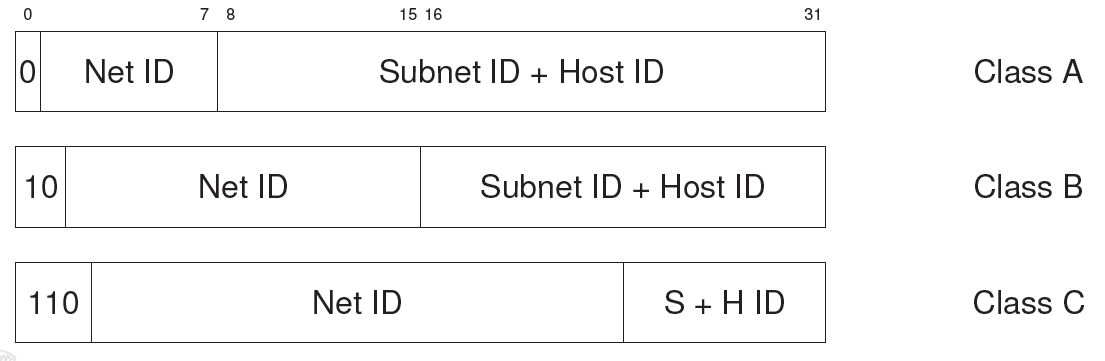
\includegraphics[scale=0.58]{img/ipv4classes.png}
    \decoRule
    \caption{IPv4 classful architecture example; some bits of the $hostID$ are used to code the $subnetID$.}
    \label{fig:ipv4classes}
\end{figure}

%----------------------

\subsubsection{Routing table}
A \textbf{routing table} is a data table stored in a router or a network host that lists the routes to particular network destinations, and metrics (distances) associated with those routes. The routing table contains information about the topology of the network immediately around it. In network security is quite important, as one of the easiest ways to deceive users is to check and take advantage of their routing table.

The routing table consists of at least the following information fields:

\begin{itemize}
    \item \textbf{destination}: the destination IP address, which can be paired with the netmask;
    \item \textbf{netmask} or \textbf{genmask}: the subnet mask that when used together with the destination gives the final network ID, needed for routing;
    \item \textbf{gateway}: also called \textit{next hop}, it is the address of the next station to which the packet is to be sent on the way to its final destination. This is the output interface, which is used in order to send packets outside. An asterisk next to it indicates that it is directly reachable through the current interface, meaning that packets must not pass through the router (otherwise packets will be sent first to the router (gateway));
    \item \textbf{metric}: the routing metric of the path through which the packet is to be sent; the route will go in the direction of the gateway with the lowest metric.
\end{itemize}

Depending on the application and implementation, it can also contain additional values that refine path selection:

\begin{itemize}
    \item \textbf{interface}: identifies the NIC associated with the corresponding network ID (e.g. \textit{eth0} for the first Ethernet card, \textit{eth1} for the second Ethernet card, etc.);
    \item \textbf{QoS flags}: quality of service associated with the route (for example, the U flag indicates that an IP route is up);
    \item \textbf{filtering criteria}: access-control lists associated with the route.
\end{itemize}

\textit{default} is a unique entry in the routing table which indicates the default route (0.0.0.0) and default gateway (which is used whenever there is no specific route in the table for a destination network address).

If two destinations have the same gateway (and the same interface), they are joined together, and the netmask is modified accordingly.

Since we cannot order the routing table in a logical way, in order to find a packet destination we need to find the best match in the routing table. If equation \ref{eq:routing} is true (a bitwise AND operation between the destination address and the netmask, which should be equal to the destination at line $i$), then entry $i$ has a rank equal to the number of 1-bits of $mask_i$; after doing this operation for all entries, we choose the one with the largest rank.

\begin{equation}
\label{eq:routing}
    destIP\; \&\&\; mask_i == destIP_i
\end{equation}

\begin{figure}[H]
    \centering
    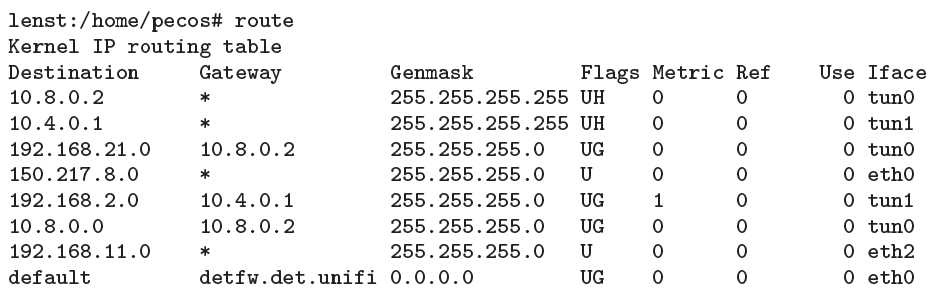
\includegraphics[scale=0.65]{img/routing_table.png}
    \decoRule
    \caption{A computer routing table example.}
    \label{fig:routing_table}
\end{figure}

\vspace{0.5em}

\emph{Example} Figure \ref{fig:routing_table} shows an excerpt from a typical computer routing table. Destination 192.168.21.0 and netmask 255.255.255.0 can be written as network ID 192.168.21.0/24.

This particular routing table has no entry for network 192.168.16.0: if it receives any packets addressed to this network, it will send them via the default gateway.

In general, whoever has the higher number of matching bits wins: suppose we want to route something to 10.8.0.2. We have two lines that match this address in the destination column: 10.8.0.2 (matches for 32 bits) and 10.8.0.0 (matches for 24 bits). The first of these addresses wins and is chosen.

\vspace{0.5em}

%-------------------------------------------

\subsection{Interconnection and data transfer}
Data is exchanged between adjacent nodes as shown in figure \ref{fig:data_transfer}; intermediate nodes should not need to process end-to-end information (except gateways and proxies).

In order to send data, the \textbf{source host} follows these steps:

\begin{enumerate}
    \item Creates a packet directed to the destination host.
    \item Checks if the destination host is in the same subnet as the source by looking at the destination IP (L3) address:
    \begin{itemize}
        \item if it is, the source uses the subnet-specific mechanisms to reach it;
        \item if it is not, the source sends the packet to an appropriate router in its own (the source's) subnet.
    \end{itemize}
    \item The underlying network does the rest (translation of addresses is done here, as this step requires a MAC (L2) address).
\end{enumerate}

Note that alphanumeric addresses have already been resolved, and we work with L3 addresses (IP addresses) from the beginning.

\begin{figure}[H]
    \centering
    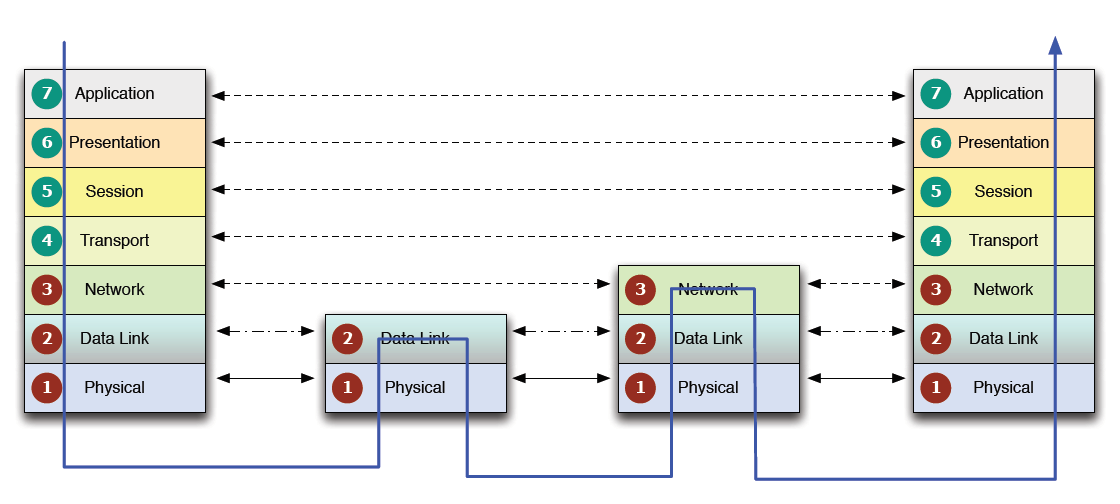
\includegraphics[scale=0.5]{img/data_transfer.png}
    \decoRule
    \caption{Data transfer in the ISO/OSI protocol stack.}
    \label{fig:data_transfer}
\end{figure}
\chapter{IPv6}
\label{ch:IPv6}
\textbf{Internet Protocol version 6}, shortened with \textbf{IPv6}, is the most recent version of the Internet Protocol (IP). It was developed by the Internet Engineering Task Force (IETF) to deal with the long-anticipated problem of \textbf{IPv4 address exhaustion}, and is intended to fully replace IPv4.

%----------------------------------------------------------------------------------------

\section{History of IPv6}
The history of IPv6 began when it was clear that sooner or later no more IPv4 addresses would be available. In short, it is mostly made of people who realized that IPv4 was a bad idea, many contradictory predictions of when the IPv4 address pool would be depleted and ultimately other predictions about the full deployment of IPv6 (which turned out so wrong that at this rate we might never even see it happen in our lifetime, or something along these lines). A simplified timeline of the most important milestones in the life of this protocol follows.

%-------------------------------------------

\subsection{IPv4 address exhaustion}
\begin{figure}[h]
    \centering
    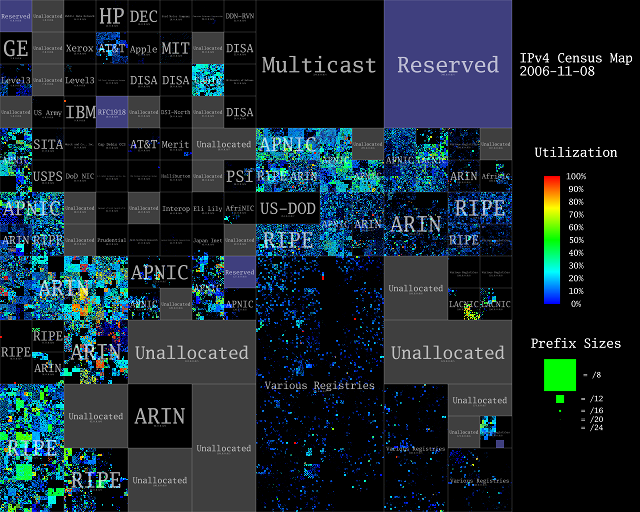
\includegraphics[scale=0.8]{img/ipv4_census_map.png}
    \decoRule
    \caption{IPv4 2006 census map, showing the distribution of IPv4 addresses.}
    \label{fig:ipv4_census_map}
\end{figure}

IPv4 address exhaustion is the depletion of the pool of unallocated IPv4 addresses. Because the original Internet architecture had fewer than 4,3 billion addresses available, depletion has been anticipated since the late '80s, when the Internet started experiencing dramatic growth.

Not all IPv4 are actually used, because many of them have been bought by people and companies who are not actually using them. However, their exhaustion was inevitable anyway because the Internet's growth has increased dramatically, not only for the high number of people who now have access to it but also because of the millions of devices online (like smartphones, IoT, etc.).

As of today (2020), IPv4 addresses are exhausted; however, they are still in wide use, so what does this mean?
Let us first understand who is consuming these addresses.

In order to use an IP address we have to \textit{own} it, and not a single one, but a block of them. So let us suppose that we are a business which, for legitimate reasons, want to have its own addresses. We go to a regional registry and ask for addresses; if there are available IPs, we pay a nominal cost (a small tax needed for the registry's operations) and get some for ourselves.

Until exhaustion, we could just go to a register and ask for a block of IP addresses; now, we have to wait in a line for weeks or months in order to obtain a new block. But wait - were not all addresses exhausted? Yes, but no: some companies that owned blocks have closed, or have released old blocks, so we can get a new one even if there are no new blocks available. Alternatively, we could also ask a company on the free market to sell their addresses to us\footnote{If UniFi would sell even just half of their IPv4 addresses, they would probably get enough money to renew a large number of their buildings: IPv4 addresses are extremely valuable.}.

On the contrary, if we want IPv6 addresses we just have to send an e-mail to the registry, and we will get as many as we want.

%-------------------------------------------

\subsection{IPv6 timeline}

\begin{figure}[H]
    \centering
    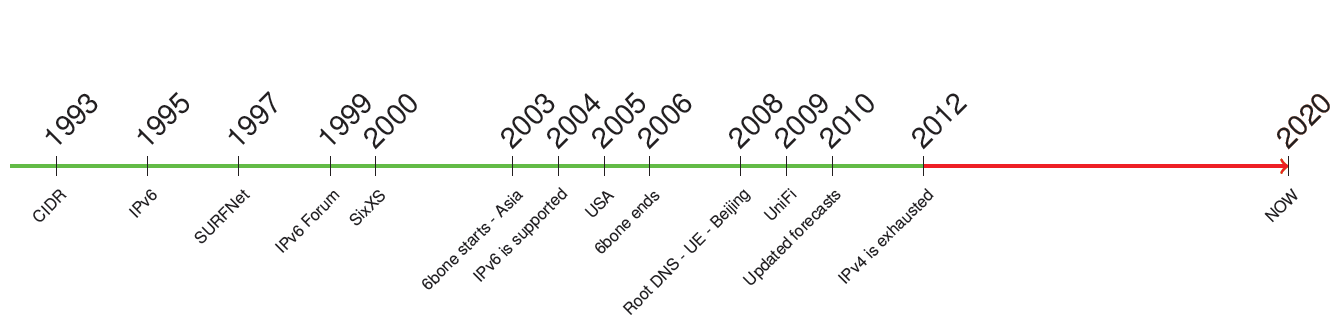
\includegraphics[scale=0.48]{img/ipv6timeline.png}
    \decoRule
    \caption{IPv6 timeline.}
    \label{fig:ipv6timeline}
\end{figure}

%----------------------

\subsubsection*{1993}
After realizing that that class-based routing was a bad idea, CIDR delays the exhaustion of IPv4 addresses by giving out smaller blocks. Before CIDR it was not possible to assign more than 254 addresses of class C (not even two consecutive block of this class), so people who required more IPs used to get a class B block, which was much larger. CIDR also helps reducing (dramatically) the routing table size.

%----------------------

\subsubsection*{1995}
IPv6 is officially released with RFC 1752. Note that as of today (2020), it is a 25-year old protocol, so not exactly a new one.

%----------------------

\subsubsection*{1997}
SURFNet, Netherlands’s academic network, goes fully IPv6.

%----------------------

\subsubsection*{1999}
IPv6Forum and regional task forces are created in order to force the adoption of IPv6; they fail miserably.

%----------------------

\subsubsection*{2000}
SixXS, one of the largest tunnel brokers, starts its operations, allowing users to connect their devices computer to the IPv6 network through it.

%----------------------

\subsubsection*{2003}
6bone, an IPv6 test bed\footnote{A \textbf{test bed} is the test execution environment configured for testing. Test beds consist of specific hardware, software, operating systems, network configurations, the product under test and other system software.}, is created to test worldwide IPv6. Japan, China and South Korea announce their willingness to become leaders in IPv6, mostly because they are heavily populated and connected to the Internet.

%----------------------

\subsubsection*{2004}
The majority of network nodes (routers) are supporting IPv6.

%----------------------

\subsubsection*{2005}
Things start to become more interesting: the USA government requires that all federal agencies migrate to IPv6 before 2008 (and they are successful). At the same time Sify, India's largest ISP, starts giving IPv6 connectivity to end users, for overpopulation reasons. Also, Tony Hain, of Cisco Systems, forecasts that between 2009 and 2016 we would say goodbye to IPv4 because of the address exhaustion.

%----------------------

\subsubsection*{2006}
6bone experiment ends successfully.

%----------------------

\subsubsection*{2008}
Root DNS can be reached also through IPv6. This is not very surprising, as DNS is nothing more than a database: no matter how we ask a query, it will answer. If we ask for a translation of an alphanumeric address, it will reply with the list of IPv4 and IPv6 addresses corresponding to that alpanumeric address. In the same year, the EU Commission sets a goal of 25\% population reached by IPv6 before 2010 (and miserably fails, because ISPs were not actually forced to do it). Meanwhile, China uses IPv6 to cover the Beijing Olympic Games; it is the biggest IPv6 use ever seen, and the transition from IPv4 is so seamless that nobody even noticed anything different.

%----------------------

\subsubsection*{2009}
The UniFi backbone goes IPv6, along with a DNS server and a webserver. % Unfortunately, unlike IPv4, the SIAF remains.\footnote{Tell me if I should remove this, but please be aware that I will be very sorry if I will have to.} % TODO Infila questa frecciatina da qualche parte pls

%----------------------

\subsubsection*{2010}
Geoff Huston forecasts update the IPv4 address exhaustion timeline to a date between September 2011 and May 2012. That also the end of the world is expected to happen during this same year, at least according to the Mayan calendar, is only a coincidence.

%----------------------

\subsubsection*{2012}
The IPv4 address pool is (finally) exhausted. The world does not end.

%----------------------

\subsubsection*{2020}
IPv6 is still being rolled out – without too many issues, but without enough security, either (it is dramatically troublesome). IPv4 addresses are still available, but there is a waiting line.

\begin{figure}[h]
    \centering
    
\includegraphics[scale=0.5]{img/ipv4_dead_meme.png}
    \decoRule
    \caption{IPv4 is dead, let it go.}
    \label{fig:ipv4_dead}
\end{figure}


%----------------------------------------------------------------------------------------

\section{IPv6 vs IPv4}
Since IPv6 is the new IP protocol version, its design goals are to fix the weak IPv4 points and enhance its strengths. It is very different and ultimately unrelated to IPv4, to the point that they can be compared to two parallel lines which never meet. For this reason, they can be used together as they will not mess up with each other (but neither will they be able to understand each other). The basic differences between them are:

\begin{enumerate}
    \item larger address space (128-bit addresses vs. IPv4 32-bit addresses\footnote{Someone could wonder why IPv4 addresses have such a short number of bits. The answer lies in the fact that no one expected the Internet to last for so long, nor to grow so fast and become as popular as it is nowadays (pretty much like nobody expects the Spanish Inquisition). It is, actually, the only case in the history of telecommunications of a network that keeps growing in time without becoming obsolete.});
    \item NATs are gone\footnote{Unless we are in extremely specific, almost non-existent contexts.};
    \item simplified packet header (dramatically faster);
    \item autoconfiguration.
\end{enumerate}

%-------------------------------------------

\subsection{Larger address space}
Suppose the green square in figure \ref{fig:ipv4_address_space} is the IPv4 address space; by comparison, the IPv6 address space would be represented by the white space around the green square, which in order to keep proportions we would have to extend outside the figure \textit{to the whole Solar System}. Another example: if we suppose an IP address to take the form of a standard grain of sand, measuring $1 mm$ x $1mm$ x $1mm$, in order to make the IPv4 address space we would need four and a half buckets of sand. For IPv6, we would need an amount of sand at least as the one necessary to cover the surfaces of six Earth planets (oceans included) with 1 $m$ of sand.

Such a humongous amount of addresses allow us to do something unthinkable in IPv4: waste them.

\begin{figure}[h]
    \centering
    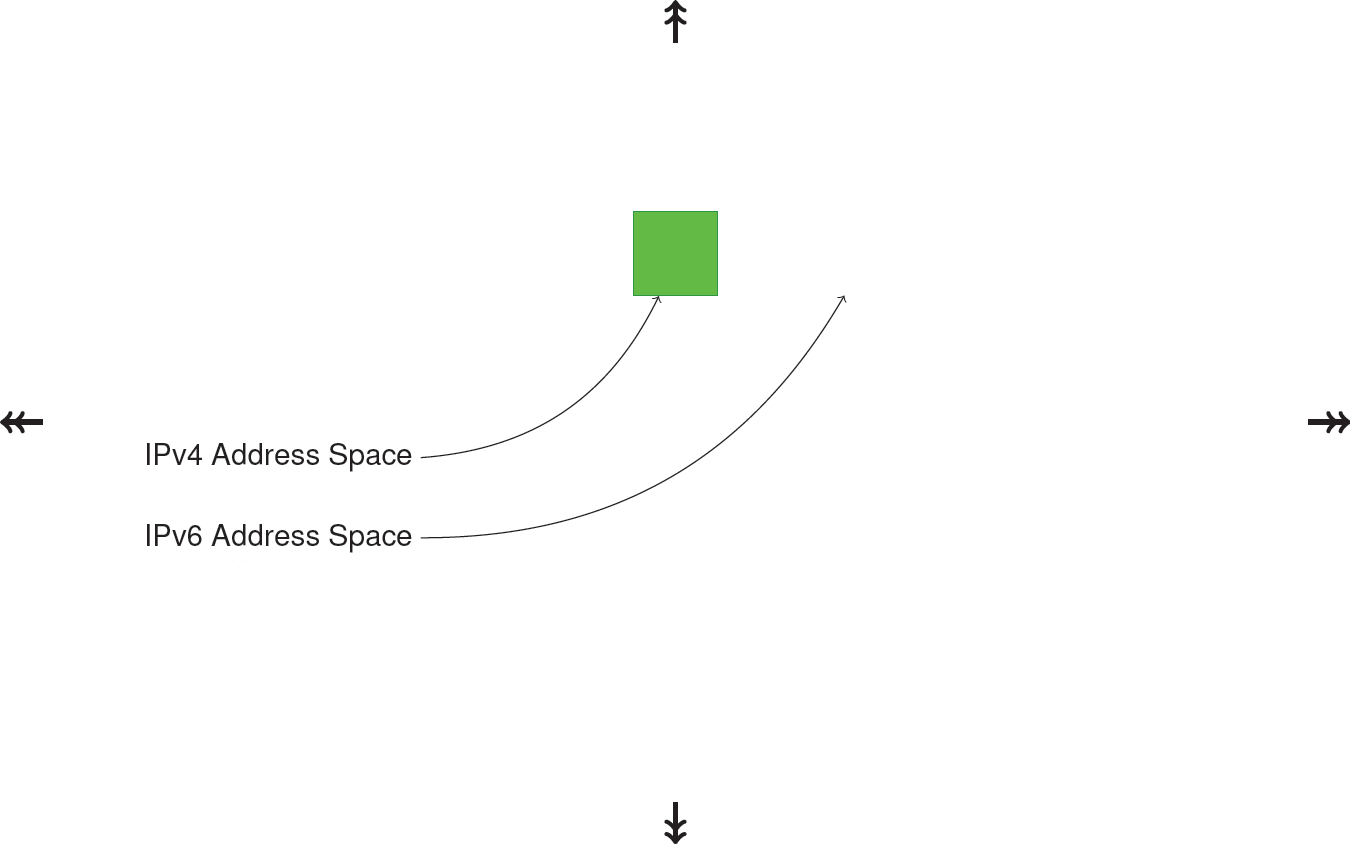
\includegraphics[scale=0.3]{img/ipv4_address_space.png}
    \decoRule
    \caption{IPv4 address space vs IPv6 address space comparison.}
    \label{fig:ipv4_address_space}
\end{figure}

%-------------------------------------------

\subsection{NATs}
In IPv4 every host connected to the Internet must have a unique address for routing. If it is not behind a NAT (Network Address Translation), then it will have a public, global address; otherwise, a host which is located in a subnet behind a NAT will have an IPv4 address which will not be unique in the global network, so it will not be able to use it for routing - in other words, the host will not be able to be reached from the outside directly.

As the name implies, NAT is an IP address mangling technique (a sort of rewriting of an IP address) used to allow multiple hosts to share the same (public) address. Basically, from the point of view of somebody outside the net, any amount of hosts behind a NAT will appear as a single IP address.

NAT allows a private IP address to reach Internet, but not the opposite - at least not in a predictable way: NATs are not deterministic, so it is not predictable if somebody from the Internet can reach a host behind one. It is also possible to bypass a NAT, even though through protocols that are either complex, difficult, dangerous or unstable.

\vspace{0.5em}

\emph{Example} The PS Remote Play application, which allows a user to play games on their PlayStation console remotely, uses techniques which allow it to bypass the NAT in order to reach the console directly - which in reality opens huge security flaws, much like creating a hole in the main door of a house.

\vspace{0.5em}

It is worth noting that we could be behind a NAT even if we have a public IP address, because sometimes ISPs use \textbf{Large Scale NATs} (LSN), very costly and unreliable machines.

To put it simply, NATs are something incredibly complex and ultimately useless, since they did not prevent the exhaustion of IPv4 addresses by limiting the number of devices directly connected to the Internet; they were also bad for security. It is thus a very positive thing that they do not exist anymore in IPv6.

%-------------------------------------------

\subsection{Simplified header}
\begin{figure}[h]
    \centering
    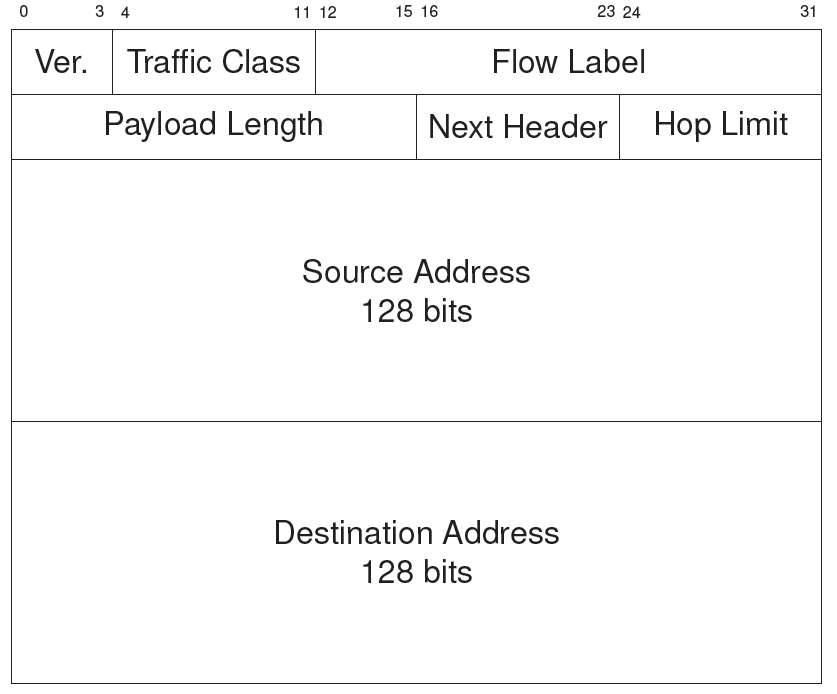
\includegraphics[scale=0.5]{img/ipv6_header.png}
    \decoRule
    \caption{IPv6 simplified packet header structure.}
    \label{fig:ipv6_header}
\end{figure}

It is possible to learn and infer a lot of things from a packet header. Protocols allow the communication between layers; their implementation lies in the header: it is the header that is carrying information, so if we remember it we implicitly know what a protocol does and if it can or cannot do something.

As shown in figure \ref{fig:ipv6_header}, the IPv6 header, with its 320 bits\footnote{IPv4 headers are \textit{at least} 160 bits long: to find the port in such a packet we must check the length of the header and then search for the layer 4 header; there is math to do, which slows down things.}, contains the following information:

\begin{itemize}
    \item \textbf{Version} (4 bits): constant with value equal to 6 (bit sequence 0110);
    \item \textbf{Traffic class} (6+2 bits): the bits of this field hold two values which have the same function as the corresponding IPv4 field. The first six bits hold the differentiated services field (DS field), which is used to classify packets, while the remaining two bits are used for Explicit Congestion Notification (ECN). In other words, this field specifies a packet's priority, so whether it should be enqueued or not, if it should follow a high quality route, and so on;
    \item \textbf{Flow label} (20 bits): a \textit{flow} is group of packets, e.g., a TCP session or a media stream\footnote{IPv4 does not have this field, and in order to check if two packets using this protocol are related we need to check the TCP or UDP ports, meaning that in cases where multiple data streams are related but do not have the same port (such as a video and audio stream sent separately but which should be played together) we have to instruct the router with complex information about how these packets should be used.}; the special flow label 0 means the packet does not belong to any flow. Note that while TCP ports consist of sequences of 32 bits (16 + 16 bits), this field only has 20 bits: this is because this number has been deemed enough in order to correctly label packets. This field is very efficient, and allows the identification of packets to be as simple as a simple XOR operation;
    \item \textbf{Payload length} (16 bits): size of the payload, including any extension headers;
    \item \textbf{Next header} (8 bits): Specifies the type of the next header, usually the transport layer protocol used by a packet's payload. When extension headers are present in the packet, this field indicates which extension header follows. The values are shared with those used for the IPv4 protocol field, as both fields have the same function;
    \item \textbf{Hop limit} (8 bits): replaces the IPv4 \textit{time to live} field\footnote{IPv4's time to live is measured in seconds (or microseconds).}. This value is decremented by one at each forwarding node, and the packet is discarded if it becomes 0. However, the destination node should process the packet normally even if received with a hop limit of 0;
    \item \textbf{Source address} (128 bits): IPv6 address of the sending node;
    \item \textbf{Destination address} (128 bits): IPv6 address of the destination node(s).
\end{itemize}

The most notable things about the IPv6 header are:

\begin{itemize}
    \item \textbf{fixed length} (40 bytes, or 320 bits);
    \item no more error checking (IPv4 had a checksum just for the header, which had to be checked at each node, slowing routing down);
    \item no more fragmentation (at least not in the header itself);
    \item \textbf{header extensions}: it is not wrong saying that IPv6, too, could have layer 4 information (ports) in the header, making things more complex to translate; the difference with IPv4, however, lies in the fact that we know exactly \textit{where} to find this information, making it an extremely simple operation. The process goes like this: after reading the first 40 bytes of a packet, the router checks if the next header has all zeros; if it finds something different from a zero (a 1), then there is one (or more) hop-by-hop extension(s) which has to be further processed, as shown in figure \ref{fig:ipv6_header_pointers};
    \item better support for QoS tags, thanks to the flow control label;
    \item native IPSec\footnote{\textbf{Internet Protocol Security} (IPsec) is a network protocol suite that authenticates and encrypts packets of data to provide secure encrypted communication between two computers over an Internet Protocol (IP) network. It is used in virtual private networks (VPNs).}: the IPv6 specifications say that every host using IPv6 has to also implement IPSec, but it actually is a really complex protocol with a complex key management (to put it simply, a nightmare), so very few systems actually use it;
    \item mobile IPv6\footnote{\textbf{Mobile IP} is the capability of a device using the IP protocol to switch from one network to another (e.g. from 4G to 3G, from a WiFi network to another, etc.) without losing connection because the IP address changes. In a ISO/OSI world this would not happen, because addresses pertaining to different layers would be logically separated (thanks to information hiding), and the session layer would manage exactly this kind of issues. IP has this issue because it exposes the layer 3 address.} greatly simplified, as it keeps the old IP address even on a new network, meaning that the connection will not drop.
\end{itemize}

\begin{figure}[h]
    \centering
    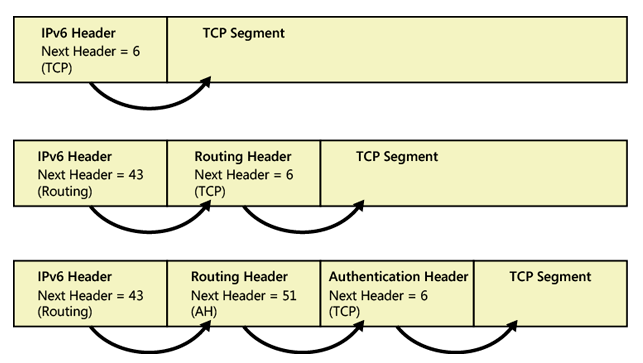
\includegraphics[scale=0.8]{img/ipv6_header_pointers.png}
    \decoRule
    \caption{
    The chain of pointers formed by the Next Header field for various IPv6 packets. In a typical IPv6 packet, no extension headers are present. If special handling is required by either intermediate routers or the destination, the sending host adds one or more extension headers. The Next Header field in the IPv6 header and zero or more extension headers form a chain of pointers. Each pointer indicates the type of header that comes after the immediate header until the upper-layer protocol is ultimately identified.}
    \label{fig:ipv6_header_pointers}
\end{figure}

%-------------------------------------------

\subsection{Autoconfiguration}
This is the strongest point of IPv6, which must never be underestimated for security purposes, because the more a system is user-friendly, the more it is actually dangerous.

The idea of IPv6's autoconfiguration is to just plug the cable in and have everything automatically working (\textbf{plug \& play}), without the user's intervention. This behavior is based first and foremost on auto negotiation of IP addresses which, unlike IPv4, is done without the help of DHCP\footnote{\textbf{DHCP}, or Dynamic Host Configuration Protocol, is a network protocol used on IP networks where a DHCP server automatically assigns an IP address and other information (namely, the subnet mask, default gateway address, domain name server (DNS) address and other pertinent configuration parameters) to each host on the network so that they can communicate efficiently with other endpoints. DHCP is an essential method to ensure that devices are able to join networks and are configured correctly, and greatly reduces the errors that are made when IP addresses are assigned manually. It can also stretch IP addresses by limiting how long a device can keep an individual IP address.} (although it can still be used in IPv6, too).

%----------------------------------------------------------------------------------------

\section{IPv6 addressing}
The IPv6 address space is so large that a new addressing scheme is needed. The two RFCs that define it are:

\begin{itemize}
    \item \textbf{RFC 4291}: defines the IPv6 addressing scheme;
    \item \textbf{RFC 3587}: defines the IPv6 global unicast address format.
\end{itemize}

IPv6 addresses are written using the \textbf{hexadecimal} format (base 16). An IPv6 network card always has several IPv6 addresses.

There are many types of IPv6 addresses:

\begin{itemize}
    \item \textbf{unicast}: one-to-one address, which can be of one of the following types:
    
    \begin{itemize}
        \item \textbf{global}: its scope is the whole Internet, and it is unique;
        \item \textbf{link-local}: it lives in the link scope, meaning that if two devices are on the same link (e.g. attached to the same switch) they will have this kind of address, which might not be unique. Also, since we have to define the link, there might be a link-local address for every network interface connected to a given device. In a multi-hop network like a wireless network, the scope of the link is the radio range of the network, so the link-local address will be valid only between one device and another that can be reached within one hop. In general, if the devices we are considering work at layer 2 (e.g. have multiple switches), then all hosts will be in the same link\footnote{A regular WiFi access point (with DHCP that gives out IP addresses) will have its devices on one link, while the ones in the wired network on a different one. However, if the access point is configured as a bridge, then everything will be on the same link.};
        \item \textbf{site-local}: deprecated, used before ULA;
        \item \textbf{unique local (ULA)}: extremely limited and specific use, as it is similar to private addresses (e.g. it is used as a temporary solution in cases where we are configuring an IPv6 address but still do not have a valid prefix);
        \item \textbf{IPv4-compatible}: deprecated;
        \item \textbf{IPv4-mapped}: an IPv6 address which has been mapped to IPv4; it is meant as a solution for the IPv6 transition, although it is not a very elegant one.
    \end{itemize}
    
    \item \textbf{multicast}: one-to-many, an address that allows a device to talk to many other devices at the same time; it is used for almost everything\footnote{In IPv4 it is not commonly used, as it is complex for routers to split the data when receivers are on different networks (and in general, it is not a simple operation), and the multicast's usefulness is extremely limited.};
    \item \textbf{anycast}: one-to-nearest; it works much like a unicast address, except that data is sent to the nearest host (so destination is decided by the router). There can be more than one device that are globally reachable at the same distance. Anycast is widely used for content delivery network products (CDN, a geographically distributed network of proxy servers and their data centers) in order to bring their content closer to the end user, because it is far more efficient than checking a list of IPv4 addresses to find out which is the nearest.
\end{itemize}

There is no broadcast address, because multicast is a lot more powerful.

%-------------------------------------------

\subsection{IPv6 address format}

The preferred format for a 16-byte global IPv6 address is as shown in the following example (extended and compact form):
\begin{center}
    \texttt{2001:0DB8:3003:0001:0000:0000:6543:210F}
    
    \texttt{2001:DB8:3003:1::6543:210F}
\end{center}

The \textbf{compact form} shown below the full one omits all leading zeros, keeping just the colons in order to avoid ambiguity in the address' length.

There also exists a \textbf{literal representation} which uses square brackets and can be used to insert the address in, for example, an HTTP address (just like we can do with an IPv4 address):
\begin{center}
    \texttt{[2001:DB8:3003:2:a00:20ff:FE18:964c]}
    
    \emph{} \texttt{http://[2001:DB8:3003:2:a00:20ff:FE18:964c]:80/index.html}
\end{center}

\emph{Example} A curious use of IPv6 prefixes, and a good example of why we can say that the IPv6 address space is so large that we can afford to actually waste addresses, is the \textbf{Debate Prefix}, or \textbf{2001:DB8::/32}. This is an address prefix that is only used for \textit{documentation}, so addresses beginning with this prefix cannot be routed (routers automatically drop packets containing them as destinations). Note that there are $2^{96}$ addresses reserved just for this purpose: a significant waste of addresses. In spite of this, this prefix is necessary in order to avoid wrongly configured networks (even at ISP levels) created by people who copy-pasted examples without changing IP addresses.

%-------------------------------------------

\subsection{IPv6 address prefixes}
The currently IANA\footnote{The \textbf{Internet Assigned Numbers Authority} (IANA) is a standards organization that oversees global IP address allocation and other Internet Protocol-related symbols and Internet numbers.} allocated prefixes are:

\begin{itemize}
    \item \textbf{\texttt{::/128}} (all zeroes): unspecified (special cases only);
    \item \textbf{\texttt{::1/128}}: loopback (there is no place like \sout{home} \texttt{::1/128});
    \item \textbf{\texttt{2000::/3}}: global unicast addresses (RFC 4291); anycast addresses are allocated from unicast prefixes, so they are indistinguishable;
    \item \textbf{\texttt{FC00::/7}}: unique local unicast, almost never used (link-local addressed are used in their place) (RFC 4193);
    \item \textbf{\texttt{FE80::/10}}: link-local unicast (RFC 4291);
    \item \textbf{\texttt{FF00::/8}}: multicast (RFC 4291);
    \item \textbf{\texttt{64:FF9B::/96}}: IPv6-mapped IPv4 address (RFC 6052);
\end{itemize}

%-------------------------------------------

\subsection{Link-local addresses}
In order to get a global unicast address we need to know some data about the network that we are joining.

The link-local unicast address, vice versa, does not require us to know anything in particular, because it is used on the local link: this kind of address is used during autoconfiguration, even when no routers are present.

\begin{figure}[h]
    \centering
    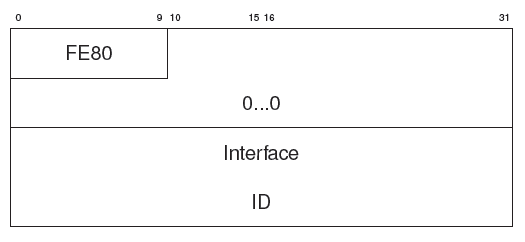
\includegraphics[scale=1]{img/ll.png}
    \decoRule
    \caption{Link-local address structure.}
    \label{fig:ll}
\end{figure}

As shown in figure \ref{fig:ll}, the first 10 bits of a link-local address are always \texttt{FE80}, while the next 54 bits are filled with zeros (could also be ones though, it would still be valid). The second part, made of the remaining 64 bits, is filled with the \textbf{interface ID}, which must be unique (every device must have a different interface ID).

%----------------------

\subsubsection{Interface ID}
The simplest way to obtain a unique interface ID is to use the MAC address of the device, since on the same link it also has to be unique for every NIC, and thus we can use this to build a layer 3 address.

However, the interface ID can also be built in other ways. For example, if we have a shorter MAC address (like in Ethernet or WiFi networks) we will have to expand it to 64 bits, thus creating an EUI-64 address.

We could also generate addresses using DHCPv6 (slightly more complex than DHCPv4 because of how hosts are identified), configure them manually or generate them with pseudo-random numbers (in this case the probability that two hosts select the same numbers is extremely low).

We can also generate it in a more creative way, like in the case of CGAs (Cryptographically Generated Address), which are generated using the 64 bits of the cryptographical signature of our data packets.

Other methods include basically anything that can be used to generate a reasonably unique address; we should make sure, however, to always double-check everything, just in case.

\begin{figure}[h]
    \centering
    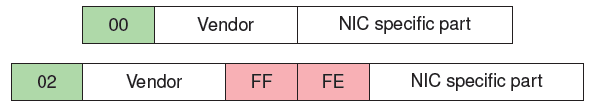
\includegraphics[scale=1]{img/autonconfexample.png}
    \decoRule
    \caption{Example of autoconfigured IPv6 address (bottom) using a 48-bit MAC address (top). The MAC address 00:1F:5B:39:67:3C maps into the IPv6 address \texttt{{\color{red} 02}1F:5B{\color{red}FF:FE}39:673C.}}
    \label{fig:autonconfexample}
\end{figure}

%-------------------------------------------

\subsection{IPv6 interfaces}
Each host (computer) with at least one NIC has \textit{at least three} IPv6 addresses:

\begin{itemize}
	\item \textbf{loopback} (\texttt{::1/128}): the IPv6 equivalent of the \textit{localhost} address in IPv4, assigned to a virtual network interface card called loopback;
	\item \textbf{link-local unicast address} (\texttt{FE80:::::}): each MAC address configured for each NIC has its own link-local address;
	\item \textbf{global unicast}\textit{s}: assigned in some way, there could be more than one per device;
	\item \textbf{all-nodes multicast} (\texttt{FF02::1}): the device might also reply to one or more multicast addresses, which are the equivalent of an IPv4 broadcast address;
	\item \textbf{all-routers multicast} (\texttt{FF02::2}): routers also have all-routers multicast address;
	\item \textbf{solicited-node multicast address} (\texttt{FF02::1:FF00:0000/104}): the core and culprit of autoconfiguration. Such an address is an IPv6 multicast address valid within the local-link, and is used in the Neighbor Discovery Protocol for obtaining the layer 2 link-layer addresses of other nodes. A solicited-node multicast address is created by taking the last 24 bits of a unicast or anycast address and appending them to the prefix \texttt{FF02::1:FF00:0/104}. We use a solicited multicast group instead of the all-node address because the all-nodes group could be too numerous, and constantly being talked to by somebody joining the network would greatly reduce efficiency; by using solicited-node multicast addresses we are limiting the target to a very small subset of the nodes.
\end{itemize}

Note that when using different addresses to specify high-level capabilities of a node, we are actually transferring layer 7 (application) functions to layers 2 and 3: a further betrayal of the principle of separation of concerns.

\vspace{0.5em}

\emph{Example} If we want to reach a printer we use an \textit{all-printer multicast address} - which is actually great, because we do not have to ask every single node if they have one of the (zillion) protocols supported by printers; instead, we send just a packet and reach all of them at the same time.

The same goes for finding a DHCP server: we send a packet to an \textit{all-DHCP multicast address} and it will reach only nodes which implement DHCP.

\vspace{0.5em}

%----------------------

\subsubsection{IPv6 multicast groups}
What does joining a multicast group actually mean?

Let us suppose that we are joining a \texttt{FF02} group: we just have to instruct our IP layer that the packets that have such an address as destination must not be discarded, but passed through the IP layer itself towards the upper layers (it is a sort of filtering). This is actually the reason why multicast addresses are more efficient than broadcasts: packets will be discarded earlier in the stack by nodes that are not routers; any node can send packets to a multicast group, but those who are not part of the group will discard packets at IP layer (in the kernel, in an earlier and faster way). In other words, IPv6 uses the broadcast address at layer 2, so if we join a link-local scope, we only have to grab the IPv6 address that we are sending stuff to, tell to layer 2 to transform it into a MAC address, and then send it. By contrast, in IPv4 the broadcast address (an IP/layer 3 address) is mapped to a layer 2 address, meaning that every node will receive it; a switch will send a broadcast packet to all ports, and all NICs will forward it to the IP layer.

It is clear thus that the node does not need anything to join a multicast group. Depending on the \texttt{02} bit, it might not even need to tell anybody: the IPv6 multicast address has a scope (reachability) defined by that bit, meaning that while \texttt{01} is \textit{interface local} (the packet will not even go outside the NIC), \texttt{02} has link-local scope. 

Other multicast scopes are \textit{realm-}, \textit{admin-}, \textit{site-}, \textit{organization-} local; these are not on a link, so packets will pass through routers and when joining one of these groups we will have to tell the router that we are part of that group.

In general, there is \sout{a shitload} quite a large number of multicast address types, and we could define even more of them.

%-------------------------------------------

\subsection{Autoconfiguration (again)}
Autoconfiguration is very simple, and very vulnerable. We have seen how to read IPv6 addresses, and that there are multiple classes of IPv6 addresses (the most important ones are global, link-local and multicast addresses). In order to better understand it, we are going to see how it works in practice.

For any node, autoconfiguration can be summarized in the following steps:

\begin{enumerate}
    \item build the \textbf{interface ID} (node ID, with any of the methods seen earlier);
    
    \item join the \textbf{solicited-node multicast address group}, and send out a \textbf{DAD} (Duplicate Address Detection) message; the DAD is not sent with the node's source address, because it still does not know if it can use it or not, so instead it uses an unspecified (all zeros) address as source. The node then waits for a response until a timeout expires; anyone who is already using that address must reply to the DAD request, while if the node does not receive anything back then it will assume that the chosen address is safe to use (implicit acknowledgement);
    
    \item start using the link-local address to check for Router Advertisements (RA), ICMP\footnote{Internet Control Message Protocol, a protocol used by network devices to send error messages and operational information indicating success or failure when communicating with another IP address.} messages periodically sent to the all-node multicast group by routers (with a \textit{still alive} kind of function);
    
    \item build a global unicast address: if there is no DHCP, RAs contain a PIO (Prefix Information Object) telling the node which prefix it can use in order to build a global address; otherwise, RAs contain a flag indicating that the node should rely on the DHCP in order to get a global address (which leads to using an all-DHCP multicast group). RAs also contain the DNS;
    
    \item send another DAD (only if there is no DHCP, otherwise the node trusts that the DHCP gave it a unique address);
    
    \item automatically set a default router\footnote{In IPv4 this was either set by the DHCP, or it had to be manually configured.};
    
    \item start surfing the Internet.
\end{enumerate}

The second step of the process represents a problem on multiple levels, because there might be a node who does use the chosen address, but replies too late. The optimal value for the timeout should then be a compromise between speed and safety, so it depends heavily on the network topology; usually, for Ethernet and WiFi it does not matter much, because replies will be in the order of milliseconds, but for long-distance/long-delay systems it is very important.

During this step the node also implicitly assumes that the DAD (which is an UDP-like packet) will be received by every node, and thus that the network is reliable; in a network with a high probability of packet loss, this system is unreliable.

Last but not least, the node \textit{also} assumes that there are no attackers that might reply in a funky way. However, if there actually \textit{is} an attacker in the network, he/she could easily prevent a node from joining the network by simply joining all solicited-node multicast groups him/herself and constantly replying to anyone else trying to join that the IPv6 address they would like to use has already been claimed. Assuming that there are no sons of bitches around, then the node will start using its own link-local address.

\vspace{0.5em}

\emph{Example} Suppose we have an interface with the IP address \texttt{FE80::2AA:FF:FE28:9C5A}. Since a solicited-node multicast address is created by taking the last 24 bits of a unicast or anycast address and appending them to the prefix \texttt{FF02::1:FF00:0/104}, the associated solicited-node multicast address is \texttt{FF02::1:FF28:9C5A}. Note how, having taken 104 bits from the address, the last byte of the penultimate field \texttt{00} is not used in the prefix.

It is interesting noting that the solicited-node multicast address prefix \texttt{FF02} is also used in the autoconfiguration for the global multicast addresses; a subset of 24 bits of the original address, however, is large enough to have an extremely small probability to get a DAD reply, even from someone with a very similar address.

\vspace{0.5em}

The DNS is usually got from the RA, but can also be:

\begin{itemize}
    \item obtained from the IPv4 stack, if there is a dual-stack;
    \item manually configured (definitely a bad idea);
    \item obtained from DHCPv6;
\end{itemize}

Note that in old machines or custom made IP stacks we have to double check that they understand RAs or DHCP with DNS, otherwise our devices will apparently work, but they will not be able to resolve addresses.

%----------------------

\subsubsection{About autoconfiguration attacks}

What happens if an attacker gets into this process? Total panic: there is no way to avoid it. The most dangerous attacks are those on the same link, where one usually assumes that no attacker can get that close to a victim. Some people proposed to secure on-link messages with a cryptographic protocol, but this would go against autoconfiguration, because it would require that every device that can join the network has already been configured for that network (given a secret). So in short, we either have autoconfiguration, or we protect ourselves from attackers: it is a short blanket.

%----------------------

\subsubsection{More about IPv6 vs. IPv4}
In general, we must forget about many concepts bound to IPv4, because they are utterly wrong in IPv6. As an example, in IPv6 there is no netmask, because the address is simply split between a net part (which is always 64 bits long) and the network interface part (made of the other 64 bits), so we cannot ever have subnets of different length and sizes.

Neighbor solicitation is another example: while in IPv4 it is enabled when two hosts share the network part, this is not always true in IPv6, because when a node has a unicast packet to send to a neighbor but does not know the neighbor’s link-layer address, it performs address resolution.

Note that in IPv6 neighbors are nodes attached to the same \textbf{link}, which is defined as \textit{a communication facility or medium over which nodes can communicate at data link layer, i.e. the layer immediately below IP}. This means that everything depends on the layer 2 physical topology, not on something that we can infer from the IP address.

The only concept that holds is \textit{on-link}, which is not based on the IP address. But still, while in IPv4 two addresses are in the same subnet if they share the same network part (and thus they are connected by a switch or another layer 2 system, and do not need a router), in IPv6 we can never infer from two IP addresses if they are attached to the same switch, if there is a router in between and/or if they can communicate directly, even if they ping each other. The on-link property is \textit{not} a consequence of having the same prefix.

\vspace{0.5em}

\begin{figure}[h]
    \centering
    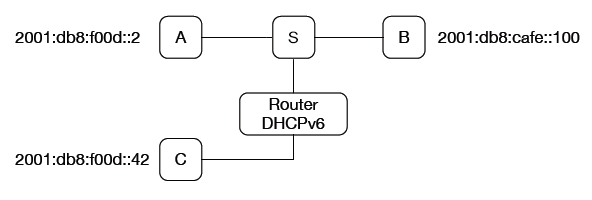
\includegraphics[scale=0.7]{img/neighbors_example.png}
    \decoRule
    \caption{IPv6 on-link example.}
    \label{fig:neighbors_example}
\end{figure}

\emph{Example} Let us consider the network shown in fig. \ref{fig:neighbors_example}: devices A and B are on the same link but have different IP address prefixes, while A and C are on different links but have the same prefixes.

In IPv4, devices A and B would not be able to communicate, because their addresses do not have the same prefix. Additionally, having A and C with the same prefix or the same network part on two different sides (physical interfaces) of the router would create a dramatic conflict: the router would be quite unhappy; it is possible, but only if he have very good hands and we build the routing table in a very specific way, not only on the router, but also in A and C - basically, it would be a bad idea.

In IPv6, vice versa, not only the network in the figure is legal, but also all devices will communicate with each other: A and B because they are on the same link (connected by switch S), while A and C because they know that they are attached to the same router.

It is the router who tells in its Router Advertisement (RA) to the A-B link that they are on the same link (connected by the router itself), by means of a prefix and an on-link bit which, if set, allows every host to assume that any other host that share the same prefix is on the same link (IPv4-alike). If the on-link bit is not set, then no host will ever assume that a given destination is on the same link, unless the router will them otherwise.

Let us suppose now that A wants to send a packet to C; since A does not assume that C is on the same link, it will send it to the router, which will forward it to C. C will do the same.

If A and B would do this operation, too, then it would be sub optimal: every packet will pass through the router, while it could simply go from A to B (and vice versa) directly, since they are on the same link.

Suppose now that there is another host D, with the IPv6 address \texttt{2001:db8:f00d::66}\footnote{Read \textit{"two-thousand debate food"}.}, on the same side as C; in this case A will send its packets to the router, which will forward them to D, and D will do the same with packets destined to A. This, too, is sub optimal, since data will have to go through the router.

\vspace{0.5em}

%-------------------------------------------

\subsection{ICMP redirect}
We said earlier that autoconfiguration is a very sensible spot of IPv6. The truth is that there is another phenomenal vulnerability in this protocol, and this is ICMP (Internet Control Message Protocol) redirect.

Through ICMP, the router can inform a device about the on-link property of a destination, effectively redirecting packets.

\vspace{0.5em}

\emph{Example} Let us consider the example in figure \ref{fig:neighbors_example} again.

Suppose that A sends a packet to B through the router. The router forwards the packet to B \textit{and} sends a message (to B) telling it that A is on-link, and giving it A's MAC address. From there on, A and B will know that they are on the same link and thus A will send packets directly to B, and vice versa.

Now, suppose that B is a router with a slightly different address (another number instead of the final \texttt{100}). If A does not know that B is the right router, it will send a packet to the main router; the main router will forward the packet \textit{and} send a message to A telling it that the designated router is B, so that from there on A will send packets directly to B.

\vspace{0.5em}

The example above explains how ICMP redirect works; the vulnerability lies in the fact that if we have an attacker on a given link that forges fake redirect messages, he/she can claim to be the router for a given block of addresses and for any host on the Internet, thus bypassing all routers after the first package (because hosts will work at switch level).

The point is that we can have completely different addresses that communicate directly if a router (or someone who poses as a router) tells them that they are on the same link.

In short, ICMP redirect is an extremely powerful mechanism, but very dangerous, too. In spite of this, it is dramatically useful and important in order to set up and maintain a network with multiple routers and addresses, because even if we could skip (filter) its messages, it would be a very bad idea.

%----------------------

\subsubsection{Countermeasures}
Given the \textit{huge} vulnerability represented by ICMP redirect, we need to have a security plan. Remember that \textit{security} is not about making things secure, but rather about defining what security means for us - and making it happen.

The steps to reach the target security must follow a precise path:
\begin{itemize}
    \item understand the enterprise architecture and its goals;
    \item define the security targets that have to be enforced (e.g. robustness, failsafe operation and percentage, admitted outage, confidentiality, etc.);
    \item analyze threats, occurrence probability and attacker capabilities;
    \item define countermeasures;
    \item measure the effectiveness.
\end{itemize}

In the case of IPv6, we have to evaluate if the link-local network can be physically touched by somebody that is not trusted (for example, the university's network is not trustable because some ports are located in rooms that are publicly accessible, like the Ethernet port in the printing room).

A countermeasure to ICMP redirect attacks could be controlling what passes through the network - physically-wise. We should check that the network cable is physically secure (e.g. in an iron tube), in order to make sure that it is always sane and cannot be touched; periodical electrical checks (a fairly common solution) could also be employed to ensure that it has not been detached and reattached.

We could also check where a packet comes from: against somebody who pretends to be a router we could install a check on the switch to see on which port is located the router, and only allow RA messages from that port (meaning that everything else is an attacker). However, in order to do this we need to have a switch able to analyze this kind of threat.

%-------------------------------------------

\subsection{IPv6 threat model}
IPv6 attacks can be divided in two main categories:
\begin{itemize}
	\item IP-level attacks and vulnerabilities;
	\item upper-layer attacks and vulnerabilities.
\end{itemize}

Upper-layer attacks and vulnerabilities are not our business, but we should always check for possible holes in the software. IPv6 addresses (and in particular IPv4-mapped ones), on the other hand, can (and \textit{will}) raise application-level vulnerabilities.

Compared to IPv4, IPv6 has some similar attacks, but also some new ones. There are many IPv4 attacks that do not apply to IPv6 anymore.

For example the fragmentation attack, which is possible in IPv4, is impossible in IPv6 - not because IPv6 does not have fragmentation, but because on IPv6 the extension header for destination is end-to-end (only the source can fragment packets): if we find a malformed packet, we can easily assume that either the sender went nuts or the sender is kinda sus, so we just trash it (fig. \ref{fig:fry_packet}).

Network scanning is also practically impossible in IPv6 if the attacker is not in the same network because of the huge dimensions of the address space - this also means that the network is harder to control, though.

Another nice thing is that NATs are gone; however, since networks still need to be partitioned, IPv6 uses more firewalls than IPv4.

\begin{figure}[h]
    \centering
    
\includegraphics[scale=0.6]{img/fry_packet.png}
    \decoRule
    \caption{A router trying to figure out if a given packet is malformed or has been tampered with.}
    \label{fig:fry_packet}
\end{figure}

The ICMP redirect attack is, vice versa, a new kind of attack that was not possible in IPv4, while ARP spoofing\footnote{Address Resolution Protocol spoofing, an IPv4 attack where an attacker is able to make a certain destination believe that he/she is somebody else.} is still there, even though in a slightly different form.

The point is that IPv6 has not been created to be secure, but only to be easier to use than IPv4; being made to be easier for the user means that it is easier to exploit for the attacker. The fact that something has been certified as secure (with a given level of security) on IPv4 does not imply a similar level of security in IPv6. Obviously, assuming that systems are similarly secure in both IPv4 and IPv6 would be a horrible mistake. For this reason, because IPv4 and IPv6 are completely unrelated, in order to check if a software/protocol is secure at layer 3 or - even more importantly - layer 7, we need to make a \textbf{vulnerability assessment}, or \textbf{vulnerability analysis} (check for memory leaks and other problems that arise from the fact that IPv6 addresses are longer) for both of them.

Remember: IPv6 is \textbf{not} more secure than IPv4; it is just \textit{differently insecure} (also, we do not even have much experience with IPv6 attacks, so it is harder to make it more secure).

\vspace{0.5em}

\emph{Example} The THC IPv6 Attack Toolkit comes with lots of effective IPv6 attacking tools; it can be found at \url{https://github.com/vanhauser-thc/thc-ipv6}.

\vspace{0.5em}
\chapter{The evil in NAT}
\label{ch:nat}
\textbf{Network address translation}, or \textbf{NAT}, is a method of remapping an IP address space into another by modifying network address information in the IP header of packets while they are in transit across a traffic routing device. The technique was originally used as a means to mitigate the IPv4 address exhaustion, since one Internet-routable IP address of a NAT gateway can be used to identify an entire private network. For this characteristic NAT is also often used to hide the internal network structure, although this is not an advantage for security.

In practice, a NAT hides an entire IP address space, usually consisting of private IP addresses, behind a single IP address in a public address space (the NAT's). The hidden addresses are changed into a single public IP address as the source address of the outgoing IP packets so they appear as originating not from the hidden host but from the routing device itself.

In order to make NAT work, some IPv4 addresses have been declared \textit{private}\footnote{A private network is a computer network that uses private IP address space (RFC 1918). Being private by definition, these addresses cannot be used for routing in public networks, because they might be (actually, surely are) duplicate.} (see table \ref{tab:ipv4_private}; the most useful range is \textbf{class C}).

\begin{table}[h]
    \centering
    \begin{tabular}{|c|c|}
        \hline
        \textbf{Class} & \textbf{Address range} \\
        \hline
        A & \texttt{10.0.0.0} \\
        B & \texttt{172.16.0.0} \\
        C & \texttt{192.168.0.0} \\
        \hline
    \end{tabular}
        \caption{IPv4 private address space.}
        \label{tab:ipv4_private}
\end{table}

Note that although NAT exists for both IPv4 and IPv6, in IPv6 it is not commonly used, so from now on it shall be implied that we only refer to the IPv4 version.

Spoiler alert: this is where I'm packing these notes with \textit{more} memes. Because I can.

\begin{figure}[h]
    \centering
    
\includegraphics[scale=0.2]{img/unlimited_power_meme.jpg}
    \decoRule
    \caption{How I feel inserting memes in the notes.}
    \label{fig:meme_unlimited_power_nat}
\end{figure}

% TODO Find out if I can insert this masterpiece meme.
%\begin{figure}[h]
%    \centering
%    
\includegraphics[scale=0.5]{img/power_pec_meme.png}
%    \decoRule
%    \caption{How I feel inserting memes in the notes.\\
%    \footnotesize \textit{Credits for this masterpiece go to Abdullah Chaudhry. No offense intended (really).}}
%    \label{fig:power_pec_meme_nat}
%\end{figure}

%----------------------------------------------------------------------------------------

\section{NAT classification}
\label{sec:nat_class}
We can define three kinds of NATs:

\begin{itemize}
    \item \textbf{static NAT} (1:1 mapping): a single address in the private pool is directly translated to the public pool, using a stateless table; basically useless, because it does not save addresses: we need as many global addresses as the devices in the local network;
    \item \textbf{dynamic NAT}: dynamically maps an address in the private area network to another address of the outside area, meaning that only devices that are actually active need a binding (an active translation); for this reason, it needs a stateful table in order to track down which devices need to get outside of the network (and which not);
    \item \textbf{NAPT}, \textbf{Network Address and Port Translation}: the system does not only change the IP number, but also the layer 4 address (the TCP or UDP port), meaning that with a single global address we can actually host and keep up something like 64.000 connections (\textit{connections}, not hosts). In this case the system is a lot more complex, because it needs to track the single end-to-end connections (the \textbf{flow}) between devices in the private network and global network.
\end{itemize}

%----------------------------------------------------------------------------------------

\section{NAPT: Network Address and Port Translation}
\textbf{NAPT}, \textbf{Network Address and Port Translation}, represents the actual NAT that can be found in most private networks. As briefly explained in section \ref{sec:nat_class}, it is a variant of the dynamic NAT that tracks flows. A \textbf{flow} is identified in TCP/IP (in both TCP and UDP) by a five-tuple made of the \textit{protocol}, the destination and source \textit{IP addresses} and the destination and source \textit{ports}. We can differentiate between two flows by a change in any of these five elements. The protocol, destination IP and port cannot actually change, except for the source address and port which are modified by a NAT.

%-------------------------------------------

\subsection{NAT and cryptography}
\textit{Timete Danaos et dona ferentes}\footnote{\textit{Beware of Greeks bearing gifts.}}: NAT violates the non-modification principle of a package. Since it changes the IP addresses and ports, we will have to
re-compute the header and the TCP/UDP checksums, and previous data that could enable us to check if a packet has been tampered with will not be usable anymore. For this reason, the IPsec protocol does not work in NAT environments: all packets would be discarded due to a failure to the security check.

\begin{figure}[h]
    \centering
    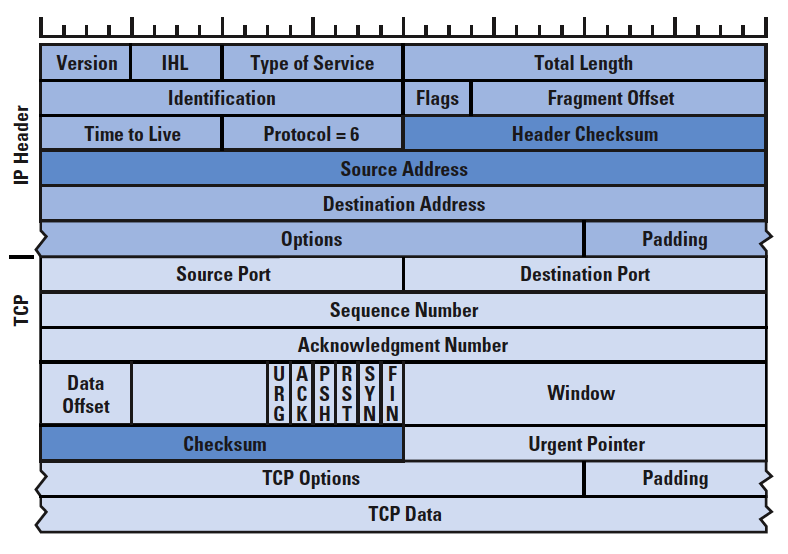
\includegraphics[scale=0.6]{img/ip_header.png}
    \decoRule
    \caption{A detailed diagram showing the IP and TCP header.}
    \label{fig:ip_header}
\end{figure}

\begin{figure}[H]
    \centering
    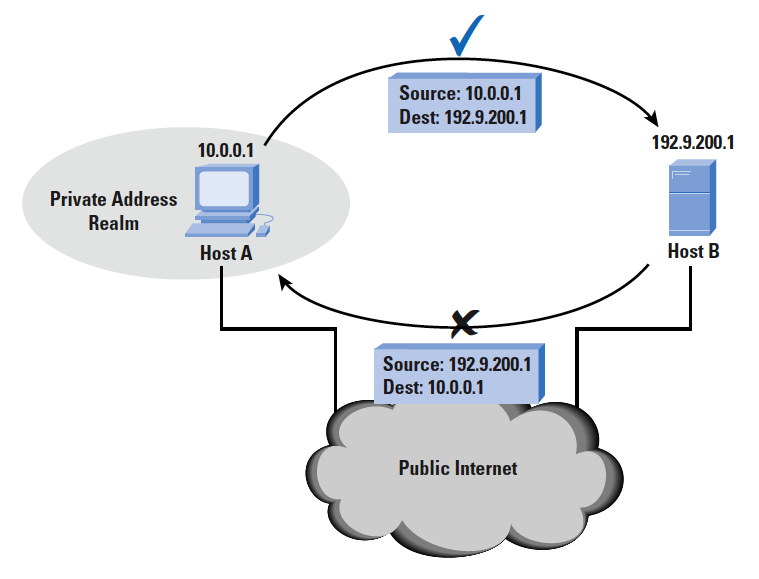
\includegraphics[scale=0.6]{img/nat_basic.png}
    \decoRule
    \caption{Using a private address to send something will get packets to their destination, but the receiver will not be able to respond to a private IP address.}
    \label{fig:nat_basic}
\end{figure}

The only way to do a checksum integrity check while using a NAT is to do it either after having passed the NAT, or inside the private network behind the NAT. An alternative, but extremely penalizing way (in terms of efficiency), is \textbf{IP-over-IP}, a technique which encapsulates an IP packet into another IP packet, so that it has two headers; we could also use \textbf{IP-over-TCP}, but all in all it kills the whole data transfer process.

%-------------------------------------------

\subsection{NAT basics}

As shown in figure \ref{fig:nat_basic}, it is also the NAT's job to change the IP header of incoming packets so as to deliver them to their intended receivers. The whole process is (usually) completely transparent to the user, and can be summarized as follows:

\begin{itemize}
    \item a packet arrives in the \textbf{internal interface} of the NAT:
        \begin{enumerate}
            \item search for a binding (a translation); does it exist?
                \begin{itemize}
                    \item \textbf{yes}: go to the next step;
                    \item \textbf{no}: create a binding;
                \end{itemize}
            \item translate the packet;
            \item forward the packet.
        \end{enumerate}
        
    \vspace{0.5em}
        
    \item a packet arrives in the \textbf{external interface} of the NAT:
        \begin{enumerate}
            \item search for a binding (a translation); does it exist?
                \begin{itemize}
                    \item \textbf{yes}: go to the next step;
                    \item \textbf{no}: \textit{drop} the packet;
                \end{itemize}
            \item translate the packet;
            \item forward the packet.
        \end{enumerate}
\end{itemize}

%----------------------

\begin{figure}[h]
    \centering
    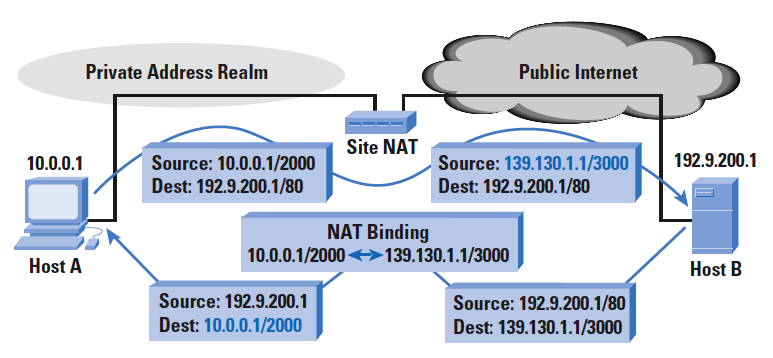
\includegraphics[scale=0.6]{img/nat_binding.png}
    \decoRule
    \caption{An example of NAT binding in a simple network.}
    \label{fig:nat_binding}
\end{figure}

\subsubsection{Bindings}
A \textbf{binding} is an entry in the NAT table that binds an internal protocol and IP to an external protocol and IP, basically specifying how to translate such a tuple:

\begin{center}
    \{IP, protocol, port\} \textit{(internal)} $\iff$ \{IP, protocol, port\} \textit{(external)}
\end{center}

It is not easy to determine if a binding is not needed anymore, so bindings have an expiration time; note that some of them can be deleted before their time expires: for example, since TCP flows can be closed gracefully, the NAT just waits for the final handshake and then removes the binding. NAT allows for 64.000 simultaneous bindings per protocol.

%----------------------

\subsubsection{Filters}
NAT \textbf{filters} decide if a packet should be translated, even if there is a binding for it. They make NAT \textbf{non-deterministic} (multiple behaviours, both good and bad), and they exist because of UDP:

\begin{itemize}
    \item \textbf{TCP} (one-on-one, two-way connection): sends and receives packets only to and from one endpoint, after a connection is established. Broadcast packets cannot be received, so every TCP packet will be translated by a NAT. TCP uses timeouts, making the connection expire after a certain time has passed since the last data has been received;
    \item \textbf{UDP} (data-based, connectionless): can receive from multiple senders without a previous connection, and broadcast meassages are allowed. It cannot be bound because there is no flow: it is not possible to decide when to delete a binding and a filter just by looking at the incoming/outgoing packets. It also introduces the demultiplexing problem: the NAT has to figure out which packet belongs to which flow, because there is only one socket (we need to ask the IP and UDP headers of the packet to check address and port).
\end{itemize}

%----------------------------------------------------------------------------------------

\section{NAT behaviours}
It is clear that the NAT must have different behaviours for TCP and UDP  - and what is worse, applications might not (properly) work if the "wrong" behaviour has been chosen. Here we describe the four types of NAT behaviour:

\begin{itemize}
    \item \textbf{symmetric NAT};
    \item \textbf{full cone NAT};
    \item \textbf{restricted cone NAT};
    \item \textbf{port restricted cone NAT}.
\end{itemize}

\begin{figure}[h]
    \centering
    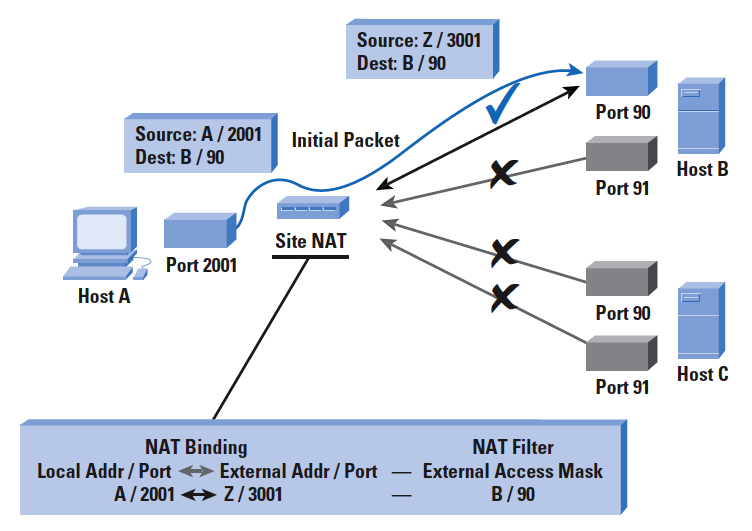
\includegraphics[scale=0.6]{img/symm_nat.png}
    \decoRule
    \caption{Symmetric NAT example.}
    \label{fig:symm_nat}
\end{figure}

%-------------------------------------------
\subsection{Symmetric NAT}
A \textbf{symmetric NAT} (fig. \ref{fig:symm_nat}) is one where all requests from the same internal IP address and port, to a specific destination IP address and port, are mapped to the same external IP address and port. If the same host sends a packet with the same source address and port, but to a different destination, a different mapping is used. Furthermore, only the external host that receives a packet can send a UDP packet back to the internal host. It works the same way for both TCP and UDP, and this is actually the only NAT behaviour used for TCP.

%-------------------------------------------
\subsection{Full cone NAT}
\begin{figure}[h]
    \centering
    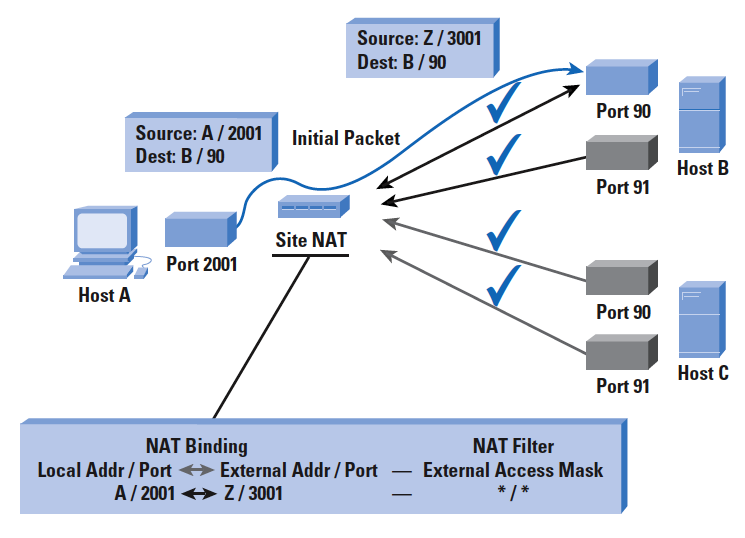
\includegraphics[scale=0.6]{img/full_cone_nat.png}
    \decoRule
    \caption{Full cone NAT example.}
    \label{fig:full_cone_nat}
\end{figure}

A \textbf{full cone NAT} (fig. \ref{fig:full_cone_nat}), the most common type of NAT, is one where all requests from the same internal IP address and port are mapped to the same external IP address and port. Furthermore, any external host can send a packet to the internal host, by sending a packet to the mapped external address. Depending on the filter, all other bindings can lead to a full cone NAT.

The security issue with this kind of NAT is that anybody can do a quick scan of the NAT server and will find which computers have something open: executing a network scan behind our network becomes a joke.

%-------------------------------------------
\subsection{Restricted cone NAT}
In a \textbf{restricted cone NAT} (fig. \ref{fig:restr_cone_nat}) all requests from the same internal IP address and port are mapped to the same external IP address and port. Unlike a full cone NAT, an external host (with IP address $X$) can send a packet to the internal host only if the internal host had previously sent a packet to IP address $X$. This kind of NAT is slightly better than a symmetric NAT, but for practical purposes is kinda useless because referral and handover\footnote{\textbf{Handover} or \textbf{handoff} is the process of transferring an ongoing data session from one channel connected to another (e.g. when a phone moves away from an area covered by one cell and enters an area covered by another cell, the call is transferred to the second cell in order to avoid call termination).} do not work.

\begin{figure}[h]
    \centering
    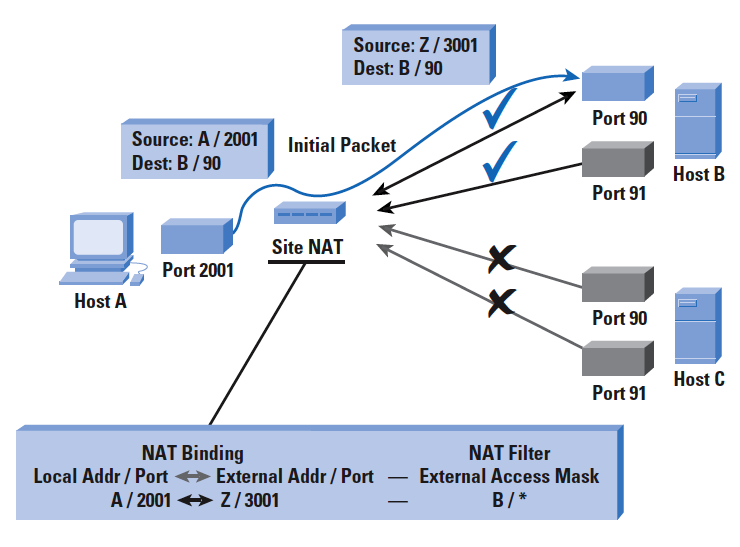
\includegraphics[scale=0.6]{img/restr_cone_nat.png}
    \decoRule
    \caption{Restricted cone NAT example.}
    \label{fig:restr_cone_nat}
\end{figure}

\begin{figure}[H]
    \centering
    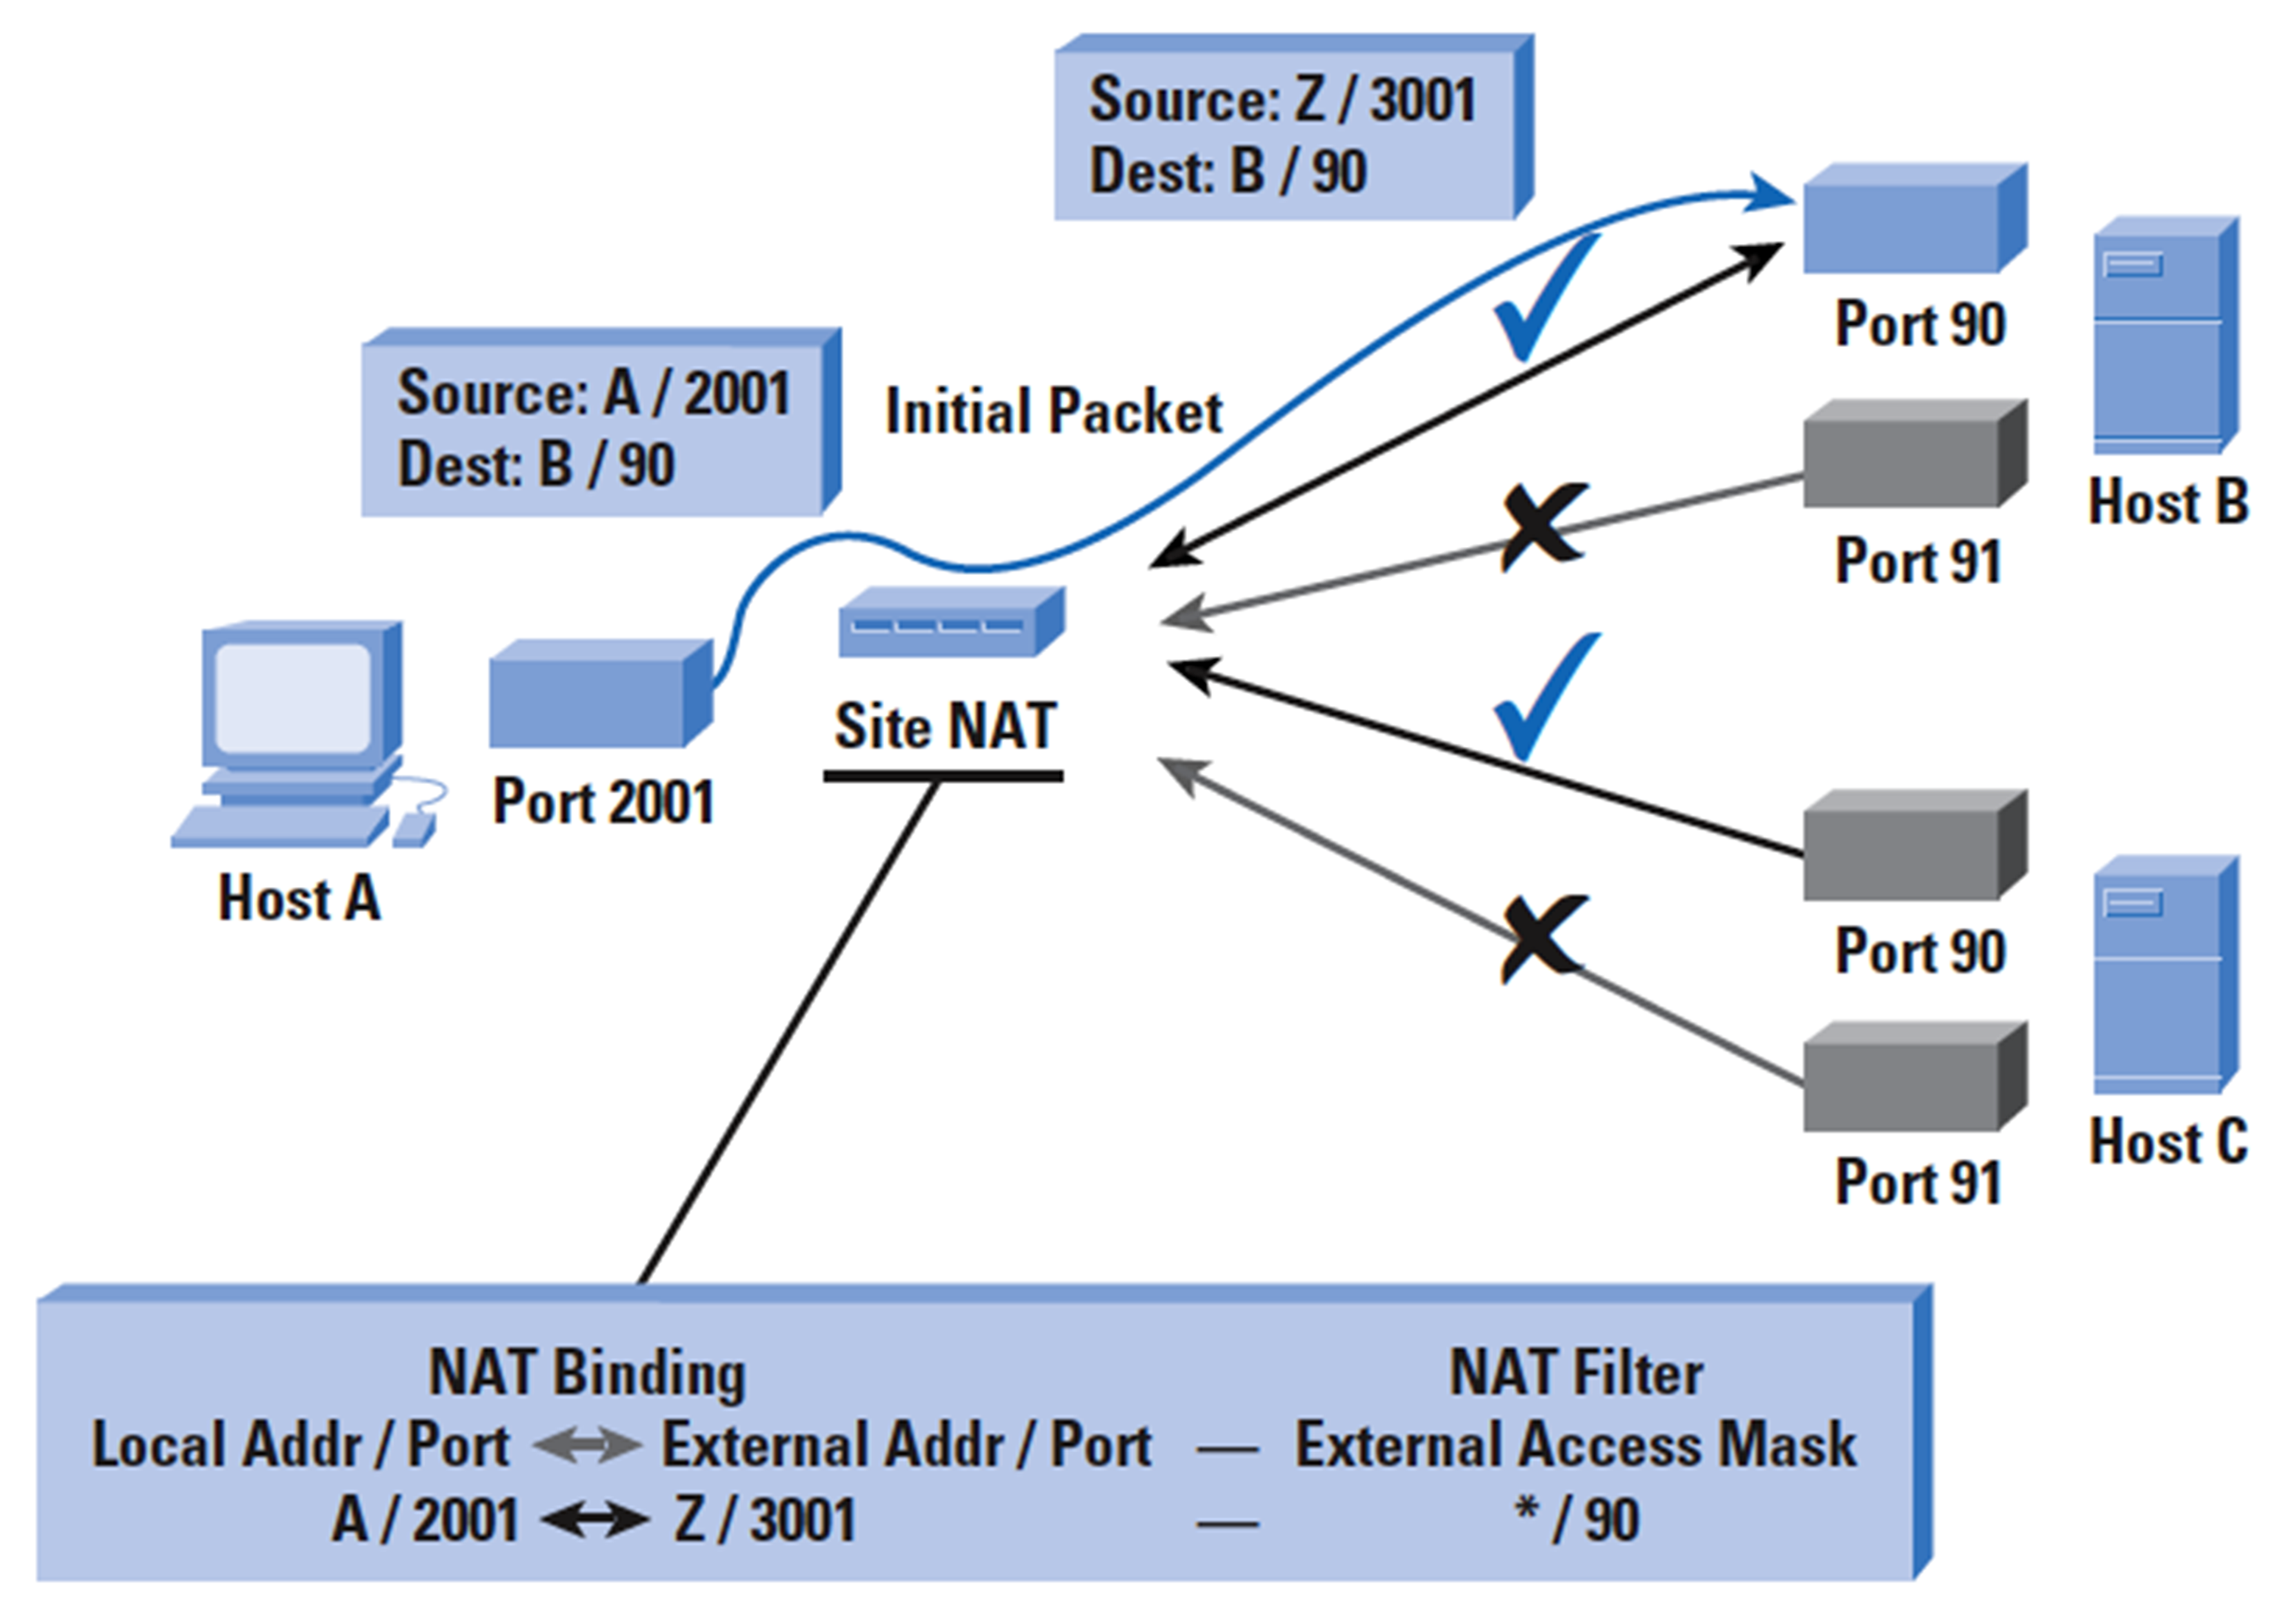
\includegraphics[scale=0.13]{img/port_restr_cone_nat.png}
    \decoRule
    \caption{Port restricted cone NAT example.}
    \label{fig:port_restr_cone_nat}
\end{figure}

%-------------------------------------------
\subsection{Port restricted cone NAT}
A \textbf{port restricted cone NAT} (fig. \ref{fig:port_restr_cone_nat}) is like a restricted cone NAT, but the restriction includes port numbers. Specifically, an external host can send a packet, with source IP address $X$ and source port $P$, to the internal host only if the internal host had previously sent a packet to IP address $X$ and port $P$.

In this kind of NAT we can still do a network scan if we know the port that must be used as source port, in order to send packets to the NAT and then have them translated towards the internal computer. However, there are more chances that the NAT or the firewall will spot suspicious activity. For this reason, UDP should be used only with this NAT behaviour.

%-------------------------------------------
\subsection{Hairpinning}
\textbf{Hairpinning} (or NAT loopback, see figure \ref{fig:hairpin}) describes a communication between two hosts behind the same NAT device using their NAT-mapped endpoint. Because not all NAT devices support this communication configuration, applications must be aware of it.

In other words, hairpinning is where a machine on the LAN is able to access another machine on the LAN via the external IP address of the LAN/router (with port forwarding set up on the router to direct requests to the appropriate machine on the LAN). 

This ability of the NAT is relevant in cases where there is a host that wants to reach another host behind the same NAT, but it only knows its (the destination's) public address.

\begin{figure}[h]
    \centering
    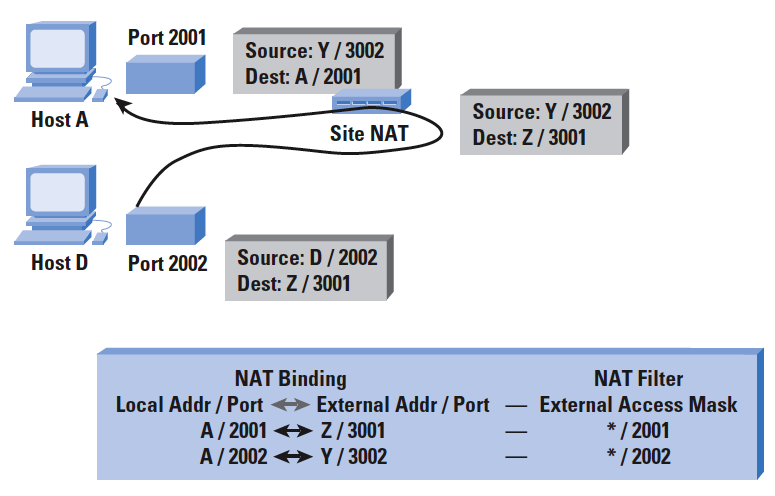
\includegraphics[scale=0.6]{img/hairpin.png}
    \decoRule
    \caption{NAT loopback (hairpinning) example.}
    \label{fig:hairpin}
\end{figure}

%-------------------------------------------
\subsection{STUN}
Sometimes we need to find out what kind of NAT we have, so that we can know if we can use certain applications. \textbf{STUN}\footnote{Rosenberg, J., Weinberger, J., Huitema, C., and R. Mahy, \textit{STUN - Simple Traversal of
User Datagram Protocol (UDP) Through Network Address Translators (NATs)}, RFC 3489, March 2003.} is just the tool for that.

STUN is a \textbf{request-reply protocol}: \textit{server, where did this packet come from?} The server replies, and STUN infers the NAT type from the answer, as shown in figure \ref{fig:stun}.

\begin{figure}[h]
    \centering
    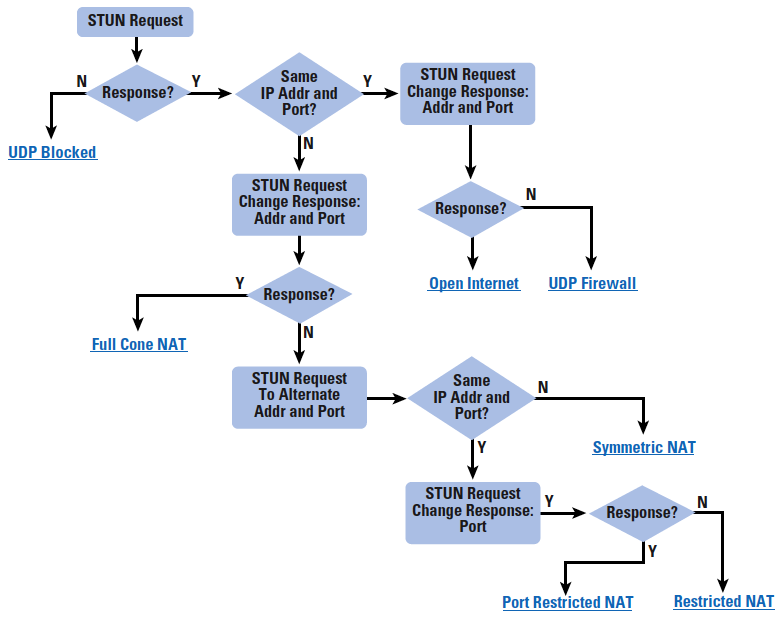
\includegraphics[scale=0.7]{img/stun.png}
    \decoRule
    \caption{STUN NAT characterization algorithm.}
    \label{fig:stun}
\end{figure}

In order to make a STUN request we need a STUN server hosted on a computer which has two global IP addresses with two open ports for each address (a capability of four total connections). The client, typically operating inside a private network, sends a binding request (through a UDP packet) to a STUN server on the public Internet. The STUN server responds with a success response that contains the IP address and port number of the client, as observed from the server's perspective.

\vspace{0.5em}

\emph{Example} Let us consider the full cone NAT shown in figure \ref{fig:full_cone_nat}. If host C can reach us from port 90, then the only possibility is that we have a full cone NAT, because that connection is only allowed in full cone; if we do not receive an answer, then we ask to use what remains (a restricted cone or port NAT). At the end of the day we can discriminate between all types of NATs.

\vspace{0.5em}

STUN is not reliable. First of all, since UDP does not provide reliable transport guarantees, a certain level of reliability is achieved by application-controlled retransmissions of the STUN requests. However, NATs are non-deterministic, meaning that their behavior can change over time; also a client might have multiple NATs one behind the other (this actually happens a lot more than one might think): in this cases, STUN might just outright fail.

%----------------------------------------------------------------------------------------

\section{More NAT classification}
\begin{figure}[h]
    \centering
    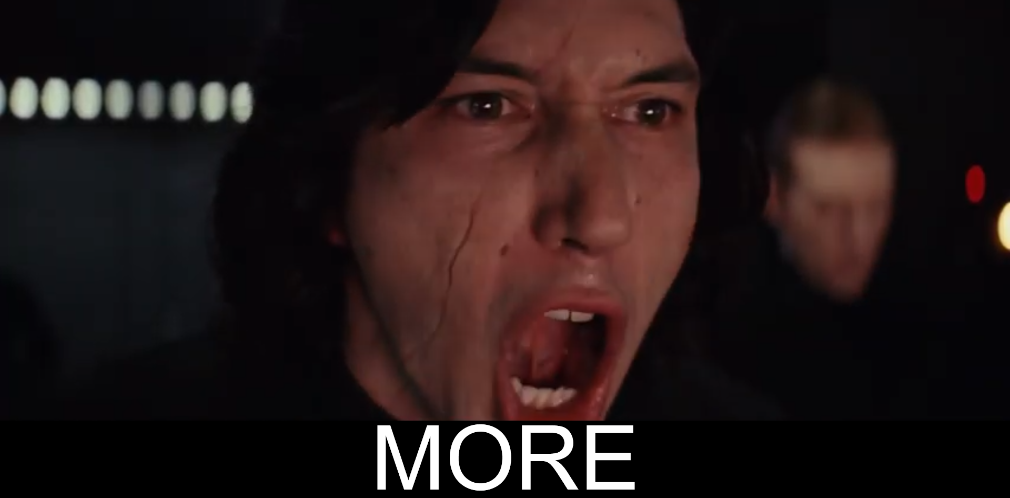
\includegraphics[scale=0.5]{img/more_meme.png}
    \decoRule
    \caption{Did you really think we were done with NAT classification? Wrong! MORE!}
    \label{fig:more_nat_meme}
\end{figure}

Now, let us clear the fact that in order to \textit{really} classify a NAT we have to check its bindings and filters. Take for example the system shown in figure \ref{fig:wut_nat}, where the NAT maps the host into two completely different things: what kind of NAT is this?\footnote{Spoiler: a shitty one.}

\begin{figure}[h]
    \centering
    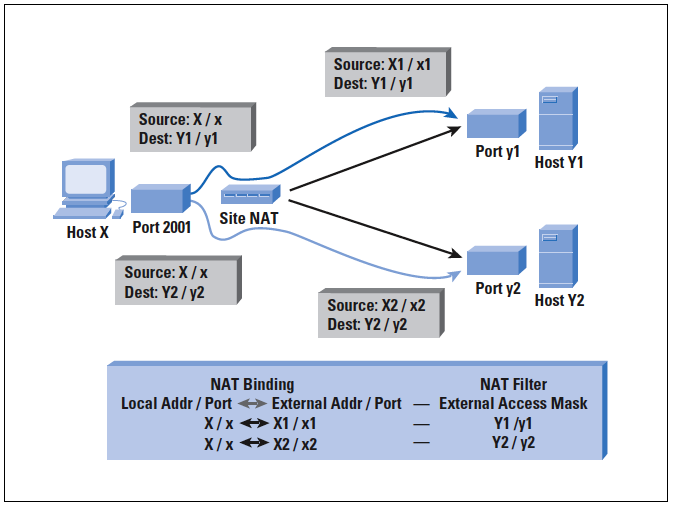
\includegraphics[scale=0.6]{img/wut_nat.png}
    \decoRule
    \caption{How the f- do we classify \textit{this}?}
    \label{fig:wut_nat}
\end{figure}

%-------------------------------------------

\subsection{Binding}
\label{nat:binding_2}
NAT bindings can belong to one of these four types:

\begin{itemize}
    \item \textbf{endpoint independent}: the NAT re-uses the binding for all packets with the same source IP/port. The
destination IP/port is not considered (full cone NAT);
    \item \textbf{endpoint address dependent}: the NAT re-uses the binding for all packets with the same source IP/port and destination IP. The destination port is not considered (restricted cone NAT);
    \item \textbf{endpoint port dependent}: the NAT re-uses the binding for all packets with the same source IP/port, and destination port. The destination IP is not considered (port restricted cone NAT);
    \item \textbf{endpoint address and port dependent}: the NAT re-uses the binding for all packets with the same 5-tuple (symmetric NAT).
\end{itemize}

%-------------------------------------------

\subsection{Port binding}
NAT port bindings can belong to one of these three types:

\begin{itemize}
    \item \textbf{port preservation}: the NAT tries to not change the port number. If two (or more) hosts use the same source port, all but the first one will have their port changed;
    \item \textbf{port overloading}: same as port preservation, the second host will win, and the binding of the first one will be discarded (ouch);
    \item \textbf{port multiplexing}: the NAT does aggressive multiplexing, trying to multiplex flows over the same port
according to the destination address/port. It can cause a lot of issues if some hosts try to connect with the same destination host. The NAT must figure out when to do multiplexing and when not to do it.
\end{itemize}

In conclusion, it is (almost) impossible to predict what the NAT will do. This is why programs usually reserve several ports (about 10-15), but it is neither logical, nor efficient or secure because every open binding allows data to go back to the sender.

%-------------------------------------------

\subsection{Timer refresh}
A NAT timer can be refreshed in the following ways:

\begin{itemize}
    \item \textbf{bidirectional}: the timer is refreshed by incoming \textit{and} outgoing packets;
    \item \textbf{outbound}: only outgoing packets will refresh the timer; depending on the application, a
keep-alive might be needed;
    \item \textbf{inbound}: only incoming packets will refresh the timer; depending on the application, a
keep-alive might be needed;
    \item \textbf{Transport Protocol state}: this one tries to decode the application-level protocol and "do the right thing" – which it often does not.
\end{itemize}

Note that all but outbound timer refreshes lead to DoS attacks. Bidirectional or inbound refreshes are not recommended because an attacker could snoop which flows are active, then keep sending packets to their bindings: perhaps those dataframes will be discarded, but in the meantime the bindings will be kept alive. This is a great way to starve the NAT to death (panic attacks).

Outbound refresh is good until we use it for streaming stuff, because we will have to send keep alive packets from the side that is not the main sender (for example the host will have to say to Netflix that is still alive, otherwise the binding will timeout - even though it is Netflix the one sending shitloads of data packets). UDP is unidirectional, so this method will not work. As for the Transport Protocol state, it has to know what is the state of a layer 7 application: the NAT can do that, and it will,  but it needs to know the protocol of the application, and layer 7 protocols are not always open source (some of them are standard and public, but many others, like Skype or Webex, are private and copyrighted, and cannot be simply reverse-engineered).

%-------------------------------------------

\subsection{External filtering}
NAT filtering includes the following modes (the same as the bindings in section \ref{nat:binding_2}):

\begin{itemize}
    \item \textbf{endpoint independent}: does not do anything (full cone NAT);
    \item \textbf{endpoint address dependent}: filter based on destination IP (restricted cone NAT);
    \item \textbf{endpoint address and port dependent}: filter based on destination IP \textit{and} port (symmetric NAT).
\end{itemize}

Remember that filters and bindings must be paired, but can behave in completely different ways. We cannot check to which category belongs the binding or port that we are using; everything depends on the amount of resources (CPU/memory) of the NAT, which will change during the day.

\begin{figure}[h]
    \centering
    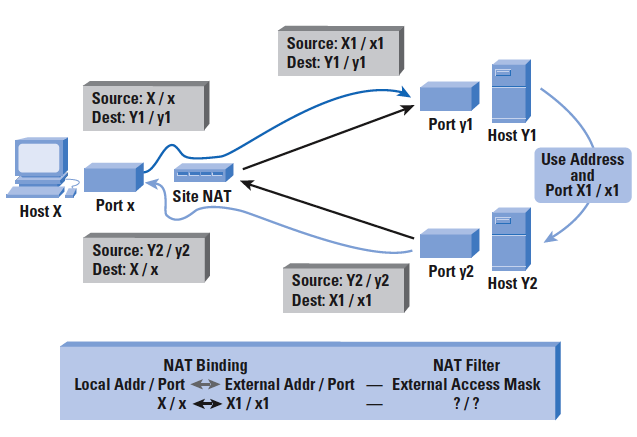
\includegraphics[scale=0.7]{img/nat_ext_filtering.png}
    \decoRule
    \caption{NAT external filtering.}
    \label{fig:nat_ext_filtering}
\end{figure}

%----------------------------------------------------------------------------------------

\section{NAT: conclusions}

%-------------------------------------------

\subsection*{P2P applications}
\textbf{Peer-to-peer}  (\textbf{P2P}) computing or networking is a distributed application architecture that partitions tasks or workloads between peers which are equally privileged, equipotent participants in the application. Nowadays every damn thing in a house that tries to be "smart" uses this technology (NAS (Network Attached Storage), smart TV and similar),  because it opens ports on the NAT, using NAT traversal techniques, since they make it easier for the user to check these devices quickly. This also means, however, that an attacker can do the same.

Basically, every binding that is open allows packets to flow back to the host; the most extreme cases happen when we have started a communication days ago and still have a binding active because of this behaviour, which makes it very dangerous.

%-------------------------------------------

\subsection*{ICMP, layer 3 encryption \& co.}
All packets that do not have specific ports, like in \textbf{Internet Control Message Protocol} (\textbf{ICMP}) messages, work by magic: instead of opening a port, they use a specific binding for that computer. If we are behind a NAT and try to send a ping to another host behind another NAT, we can do it (one device at a time).

%-------------------------------------------

\subsection*{IP fragmentation}
In order to translate packets we have to check the layer 4 header, but fragments do not contain this layer (because it only appears in the first packet). For this reason, NATs have to check the fragment ID or reconstruct the fragment. Either cases are not very nice: fragment ID needs an even more complex machine, and rejoining the packet inside the NAT introduces latency, more memory requirements, and in the end the risk of resource starvation.

%-------------------------------------------

\subsection*{UPnP and IGD}
An \textbf{Universal Plug and Play} (\textbf{UPnP}) compatible device from any vendor can dynamically join a network, obtain an IP address, announce its name, convey its capabilities upon request, and learn about the presence and capabilities of other devices.

The problem with this one is self-explaining: UPnP allows a program/host/application to forcefully open a binding, meaning that the application can ask the NAT to assign them a specific port - which in turn leads to having specific and very well known ports (not only by us, but also by attackers) permanently open on the NAT.

The \textbf{Internet Gateway Device Standardized Device Control Protocol} (\textbf{IGD}) worsens the situation as it allows an UPnP device to discover the external IP address used by the NAT and to automatically create bindings and filters.
\chapter{Attacks and vulnerabilities}
\label{ch:attacks_vulnerabilities}
This chapter reviews the main sources of vulnerabilities and attacks, from Kerckhoffs' principle to \sout{hackers} attackers.

%----------------------------------------------------------------------------------------

\section{Kerckhoffs’ principles}
\textbf{Auguste Kerckhoffs}, a Netherlands born cryptographer, wrote in his 1883 essay \textit{La Cryptographie Militaire} six principles of practical cipher design:

\begin{enumerate}
    \item The system should be, if not theoretically unbreakable, unbreakable in practice.
    \item \textbf{The design of a system should not require secrecy, and compromise of the system should not inconvenience the correspondents.}
    \item The key should be memorable without notes and should be easily changeable.
    \item The cryptograms should be transmittable by telegraph.
    \item The apparatus or documents should be portable and operable by a single person.
    \item The system should be easy, neither requiring knowledge of a long list of rules nor involving mental strain.
\end{enumerate}

In spite of being more than 130 years old, some of these principles still hold.

%----------------------

\subsubsection*{First principle}
An evergreen. It is ok if our cryptographic system is not perfect; perfection is hardly achieved, and brute force attacks are always possible. However, any feasible attack should need too much time to be performed, in order to make eventual intel unneeded.

%----------------------

\subsubsection*{Second principle}
As already stated in section \ref{sec:internet_threat_model}, the most important among these six rules, simply called \textbf{Kerckhoffs’ principle}, is the second one, which in other words says that \textit{security by obscurity} is a very bad idea.

We should never employ an unnecessarily complicated system, because we must never rely on the fact that an attacker does not know how the system works (he/she might be an intern), and when information about the system's structure leaks it makes it go from secure to completely unsecure. Also, as security is to be found in the design, we cannot even change it very often.

\vspace{0.5em}

\emph{Example} During World War 2 the Germans used Enigma, an extremely complicated machine, to secure their communications. When the British found one of those machines - not even a full one, but a reduced version - they reverse engineered it and broke the whole cryptography system.

\vspace{0.5em}

\emph{Example} There are companies that only share certain parts of the datasheets of their devices, resulting in a documentation with missing pages. These pages, which usually contain cryptography algorithms or other sensible information, are provided to the customer only after signing a non-disclosure agreement. They can often be found on Russian websites, though (see fig. \ref{fig:pirate_free_things}). However, industrial systems can still rely on security by obscurity because they have armies of lawyers: if anyone breaks such a system they will have them knocking at their door in no time - and lawyers are way nastier than the poopoos, especially when the system-breaker is a regular person and not some large organization.

\begin{figure}[h]
    \centering
    
\includegraphics[scale=0.5]{img/pirate_free_things.png}
    \decoRule
    \caption{You know how this goes.}
    \label{fig:pirate_free_things}
\end{figure}

%----------------------

\subsubsection*{Third principle}
The security of a system lies in its key. This was a good principle 130 years ago, but nowadays it is not very relevant because tasks are done by computers, and they do not have any problems in memorizing long keys.

It is worth saying that the point of stealing account passwords is to create databases, with the idea to later use them in brute force attacks. Having a number, a letter and a special character in passwords is not a good idea anymore; it is not the length of the password that makes it strong, either: the password's strength relies in randomness, and in the fact that it should be unrelated to anything else in the same dictionary (also, do not use the same password for all sites).

%----------------------

\subsubsection*{Fourth principle}
Irrelevant in 2020.

%----------------------

\subsubsection*{Fifth principle}
Irrelevant in 2020.

%----------------------

\subsubsection*{Sixth principle}
Cryptography should not be rocket science from the point of view of the user.

%----------------------------------------------------------------------------------------

\section{Outsourcing}
\textbf{Outsourcing} is an agreement in which one company hires another company to be responsible for a planned or existing activity that is or could be done internally, and sometimes involves transferring employees and assets from one firm to another. 

Nowadays we are constantly outsourcing something (e.g. cloud systems); lots of systems and/or services (a network, storage, service, anything) have \textit{at least} three entities involved: a \textbf{service customer}, a \textbf{service provider} (which could also outsource to someone else) and a \textbf{network operator}.

The \textbf{service provider} operates the service and its components, which in turn use the network infrastructure to reach the customer.

The \textbf{service customer} can customize the service and its components according to the contract with the service provider (usually only in the framework given by the service provider). It uses the service, and is not interested in how the network works.

The \textbf{network operator} builds, maintains, and runs the network infrastructure, which must respect the Quality of Service\footnote{From the point of view of security, QoS also means that data should not pass through untrustable countries, like China.} required by each service. The network operator should not be involved with the service.

%-------------------------------------------

\subsection{Service Level Agreement}
The \textbf{Service Level Agreement}, or \textbf{SLA}, is a written contract which states the goals of a service, the penalties for not meeting them and the limits. In other words, it defines what we can expect from a service, so as security analysts, we must check if there is anything related to data breaches, security, cryptography and - of course - privacy.

\begin{figure}[h]
    \centering
    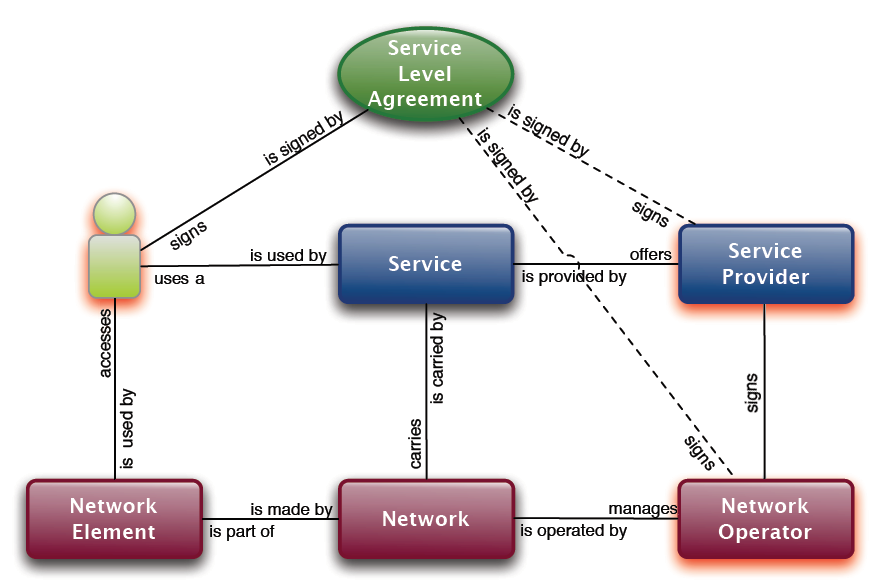
\includegraphics[scale=0.5]{img/sla.png}
    \decoRule
    \caption{Service Level Agreement diagram.}
    \label{fig:sla}
\end{figure}

The SLA is signed by the user (e.g. \textbf{EULA}, \textbf{End-User License Agreement}), and can be found between the user and the service provider. It is not uncommon, though, to have a SLA also between the service provider and the network operator, because if the latter is not involved in this agreement the security of a system cannot be fully enforced.

\subsubsection*{Vertical services}
It is much, much simpler if the service provider communicates with the network operator and tells them what kind of QoS or protection they need; this makes a service \textbf{vertical}.

A vertical service is bad for competition (thus a bad idea, especially in the long term), because whoever provides a service and has made an agreement with the network operator will have an advantage over his competitors.

\vspace{0.5em}

\emph{Example} We cannot watch Sky over a network that is not provided by Fastweb.

\vspace{0.5em}

%----------------------

\subsubsection*{Horizontal services}
If there is no SLA between the service provider and the network operator, then the diagram obtainable by modifying figure \ref{fig:sla} would be typical of \textbf{horizontal services}, like the ones built on the Internet. Here the customer can use a variety of services without knowing who their network operator is.

\vspace{0.5em}

\emph{Example} If we want to watch Hulu, Netflix, Sky, etc. we do not have to ask what is our network operator, we just go on the Internet and use them. If we use Outlook Mail but want to switch to Gmail, we can just change them.

\vspace{0.5em}

This scheme is good for competition, but since in horizontal services the network operator is not involved with the service provider, we must have a very good agreement with the network operator in order to get the best quality of service.

\vspace{0.5em}

\emph{Example} Suppose that we normally browse e-mails, but also and watch TV over Internet between 6 AM and 2 AM. We can tell the service provider what we are doing, but there is no way for us to ask the network operator for a larger bandwidth for movies (so as to adapt to the service that we are using in that moment). The network operator does not know what services we are using; it could, but it is not its job to do this: it is not interested in this, and even worse, we have to negotiate with them for good SLAs for our services.

\vspace{0.5em}

%----------------------

In cases where an extremely secure system is needed the rule of thumb is to not go towards full vertical services, but still sign a SLA between the network operator and the service provider. That is because in spite of, for example, a data center's security, the real problem lies in the transportation system, the network: an attacker is almost never close to source or destination, but is to be found somewhere in between.

%-------------------------------------------

\subsection{Hackers}
\begin{center}
\textit{A computer hacker is any skilled computer expert that uses their technical knowledge to overcome a problem. While "hacker" can refer to any skilled computer programmer, the term has become associated in popular culture with a "security
hacker", someone who, with their technical knowledge, uses bugs or exploits to break into computer systems.}
\end{center}

The term \textit{hacker} dates back to the 1960s, and is outdated;  per se, the term indicates somebody that hacks something else, or that is able to take a system, open it (physically), disassemble and reassemble it. Nowadays this word should \textit{never} be used, because it is way too generic for real security purposes. If somebody tells us that he/she has been attacked by hackers, they either have not been attacked at all or they have no idea of what that means.

In this section we will make a portrait of our attacker. In order to do this we must refer to the \textbf{hat color}, which gives a good characterization of the \textbf{purpose} of an attack (the one thing we are interested in).

The most dangerous attackers are the script kiddies, because they do not know what they are doing, while the most harmful ones are the black hats, because they \textit{do} know what they are doing. Finally, the most costly attackers are the white hats, because they will provide a long list of things to fix.

%----------------------

\subsubsection*{White hat attackers}
Their goal is to \textit{not} cause harm. These are the people who disassemble the system and tells us what is wrong with it.

%----------------------

\subsubsection*{Black hat attackers}
Their goal is to cause harm, possibly without leaving traces.

%----------------------

\subsubsection*{Grey hat attackers}
Things are not always black and white: these attackers are sometimes white, sometimes black.

%----------------------

\subsubsection*{Blue hat attackers}
These attackers are interns of a company, and work against a red team. The red hats work in security, while the blue ones try to break their system; in practice they are a sort of testers. White hats are sometimes called by companies to do this job.

%----------------------

\subsubsection*{Script kiddies}
\begin{center}
    \textit{Forgive them because they don't know what the fuck they're doing.}
\end{center}

While white and black hats tend to go against unknown/unusual vulnerabilities and are able to conceal themselves and not leave traces (at least not until it is too late), script kiddies, on the other hand, are those who use ready-to-make attacks (like the ones found on certain Linux distributions), without understanding the theory behind or even just what they are doing - or even if they do, they did not create their own tools.

Script kiddies (fig. \ref{fig:hackerman_attacks}) are the most common kind of attackers as well as the most dangerous, because they exploit known vulnerabilities that have been usually forgotten from patches and can unknowingly destroy important stuff while doing their thing.

Script kiddies are pretty much like mosquitoes: not very dangerous, but since there are many of them they are very annoying. Fortunately, they are preventable.

\begin{figure}[h]
    \centering
    \includegraphics[scale=0.2]{img/hackerman.png}
    \decoRule
    \caption{This is what script kiddies think they look like (but they really don't).}
    \label{fig:hackerman_attacks}
\end{figure}

%----------------------

\subsubsection*{Hacktivists}
These attackers are extremely dangerous: they have a goal, a message to send to the world, and like anybody with a greater goal they do not think much about the real consequences of their actions.

\vspace{0.5em}

\emph{Example} People against the animal fur industry have found out that in a nearby town there is a place where animals are grown in order to be slaughtered for their fur. They go there and free those animals: they are hacktivist by all means, because they do no understand that in doing so they have released into the environment non-native animals which are not even used to live in the wild, resulting in a greater damage to the ecosystem.

\vspace{0.5em}

\emph{Example} A notorious group of hacktivists, Anonymous, started a campaign against pedophiles, and hacked pedophile websites and disrupted them. At a certain point the international police went to one of their spokespersons and asked them to stop, because in doing so they had deleted years of investigations aimed at jailing those people.

\vspace{0.5em}

Hacktivists have the means and the goals, but sometimes they cause significant side effects or, in some cases, they are plainly against the goal of somebody else (they want to impose their view to everybody else).

%----------------------

\subsubsection*{Nation states}
NSA and Israelian, Chinese, Russians, Italian Secret Services, etc. are all groups founded by governments, which have tools beyond our reach. Defending from any one of them is somewhat possible, but ultimately is not really effective: if they want it, they will break it. Also, there are a lot of nation state-sponsored hacking groups. Their attacks are possible, effective, and we will probably not be able to defend against them.

In a risk assessment for an industrial system we would have to consider them, but we could only pray to never have to cope with them; normally we would spend too much in order to defend against them, so we would simply not consider them at all.

%-------------------------------------------

\subsection{Vulnerabilities}
The only system without vulnerabilities is a computer which has been turned off and disassembled, and every part has been individually put in a different safe, each of which placed at different locations. In fact, even this might not be enough. 

There are no systems without vulnerabilities\footnote{There \textit{might} actually exist a few systems without vulnerabilities, but it could also be just a matter of time until somebody finds a bug in them, too.}, and any really secure system is a useless one (because it does not exist). Every application contains at least a bug and an instruction that could have been left out. By induction, all programs could be reduced to a single, \textit{wrong} instruction.

Vulnerabilities stem from many different reasons:

\begin{itemize}
    \item by \textbf{design};
    \item by \textbf{\textit{bad} design};
    \item by \textbf{\textit{bad} implementation};
    \item by \textbf{\textit{bad} deployment};
    \item by \textbf{library/OS update};
\end{itemize}

%----------------------

\subsubsection*{Vulnerabilities by design}
A \textbf{vulnerability by design}, as the name implies, arises from the way in which the system has been designed. In these cases the vulnerability is well known and accepted; the choice to allow such a flaw in the system is usually motivated by simplicity, compatibility and other similar reasons (in many cases the system would not work if the vulnerability would have been patched).

Examples of vulnerabilities by design include:

\begin{itemize}
    \item resource discovery protocols;
    \item ARP/NDP;
    \item NAT.
\end{itemize}

%----------------------

\subsubsection*{Vulnerabilities by \textit{bad} design}
A \textbf{vulnerability by \textit{bad} design} arises from a fundamental mistake or oversight in the software's design. Often these vulnerabilities are caused by badly implementing a standard. In these cases, even though the programmer pays attention to every single line of code, reads the documentation and does everything that is possible in order to avoid mistakes, more often than not it is the standard itself that is written in a dramatically obscure, unclear or even missing way. This is either because whoever wrote it did not realize that they did not explain it in a decent way, or because they intentionally wanted to give advantage to some implementers by leaving out fundamental details from the public standard and then giving them to a few chosen people (for commercial purposes; an example of this is the 5G standard, of which only those who contributed to it know all the details).

Examples of vulnerabilities by bad design include:

\begin{itemize}
    \item SAMBA (Windows file sharing);
    \item attacks on speculative executions in CPUs\footnote{Speculative execution is an optimization technique where a computer system performs some task that may not be needed.};
    \item errors in the management sequence for exceptions.
\end{itemize}

%----------------------

\subsubsection*{Vulnerabilities by \textit{bad} implementation}
There are \textbf{vulnerabilities by \textit{bad} implementation} because coders are underpaid, and because the release cycle of software is too fast. Programming done right would require two people in front of a monitor and full tests for every single test case, but companies are not willing to pay the price of making robust software, so nobody does that.

The only cases where software is super-checked is that of avionics systems (military aircrafts) - but even they could still contain important vulnerabilities (e.g. the Orion capsule failure\footnote{Orion (officially Orion Multi-Purpose Crew Vehicle or Orion MPCV) is a class of partially reusable space capsules to be used in NASA's human spaceflight programs. On November 30th, 2020, it was reported that NASA and Lockheed Martin had found a failure with a component in one the Orion spacecraft's power data units which casts uncertainty on a November 2021 launch date, since it could take months to fix.}).

There are countless examples of vulnerabilities by bad implementation, including:

\begin{itemize}
    \item incomplete if/then/else clauses;
    \item memory copies left unchecked;
    \item input left unchecked.
\end{itemize}

Countermeasures to this kind of vulnerabilities are writing tests and documentation, and giving implementers and coders enough time and resources to do a good job.

%----------------------

\subsubsection*{Vulnerabilities by \textit{bad} deployment}
\textit{Bad} deployment happens whenever we have foreseen an event in the design, but the people who deployed it did not read the docs and thus did not account for it. Basically, the system works just fine in the laboratory and test bed, but not on the field.

A possible countermeasure against this vulnerabilities is to, well, read the manual. Carefully.

%----------------------

\subsubsection*{Vulnerabilities by library/OS update}
These vulnerabilities are to be found not in the application itself, but in the libraries and/or the operating system it uses. They are more common than one might think.

Examples of library vulnerabilities include:

\begin{itemize}
    \item use of deprecated/obsolete functions (usually signalled by warnings at compilation time; deprecation means that that function has been found to be bugged and/or is not maintained anymore, and sometimes it might even be empty and only consist of a signature);
    \item random numbers actually not very random (correlation).
\end{itemize}

Countermeasures include containers and virtualization, which isolate the system.

\vspace{0.5em}

\emph{Example} If we are developing a Python application, we can use a virtual environment so that we can install new packages without messing up existing ones; we can develop and test the code by making sure that nothing, except ourselves (when updating an existing library or installing a new one), will ever mess up with the underlying system.

\vspace{0.5em}

%----------------------

\subsubsection*{More about vulnerabilities}
An alternative classification of vulnerabilities goes by \textit{"I know about it"} and \textit{"Oh shit, I didn't know about it"}.

Since vulnerabilities are extremely important, there are initiatives that pay people to find them (bug/vulnerability bounty, vulnerability hunting, etc.).

Finding new vulnerabilities, however, is not easy: we have to put the system in a controlled environment, test it, find any problem and then what vulnerability it leads to. The final prize then depends on how good was the report, if the vulnerability has already been reported, etc.; the reward for having found a vulnerability can go from the price of a pizza to that of a brand new car (even hundred of thousands of dollars, upfront cash).

There are entire databases of known vulnerabilities, among which the most important is the \textbf{CVE}, \textbf{Common Vulnerabilities and Exposures}\footnote{\url{https://cve.mitre.org/}}. It contains full descriptions and consequences of not patching a vulnerability of hundreds of past problems that afflicted software.

CVE is not meant to be a shame wall for companies that did something wrong\footnote{It actually is if the company has a long list of bugs but, yeah.}. It has been made in order to allow sysadmins to check if their system is vulnerable to something, and what are the countermeasures, which often are easier than patching or updating the whole thing (e.g. in big industries it is better having a known problem, one that we know how to avoid, rather than a system that does not have any problems but might have older ones that we do not know about). Vulnerabilities entered into the CVE attain to the ethics of white hat hacking, as CVE contains only patched bugs.

In general, the way of communicating a bug after finding it is fundamental. A white hat hacker writes a report, sends it to the relevant party and does his/her best to reach it until they give them feedback. In any case, the hacker cannot publish the vulnerability, unless either the company told him/her that they do not trust them or do not care, or he/she did not get an answer in a long time (from about six to nine months). A white hat hacker could also publish a vulnerability if they also found that it is actively being used in the wild, although this is a borderline case.
\chapter[The identity issue]{Who's who? The identity issue}
\label{ch:identity}
\textbf{Identity} is a fundamental component of security; we cannot presume to realize a secure system if we do not take into account this issue, because we must know \textit{who is who}. The very basic idea of security is to allow authorized people to do their stuff, and forbid everybody else from doing the same things - and this requires \textbf{identification}.

%----------------------

\subsubsection*{Recap}
We saw in chapter \ref{ch:intro_crypto} many different ways of securing a communication between two (or more) people or devices:

\begin{itemize}
    \item \textbf{HASH}: useful only when using different channels;
    \item \textbf{HMAC}: safer than HASH, but we need a secret key;
    \item \textbf{symmetric cryptography}: good, but we need a secret key and, more importantly, cannot tell who is who (we cannot trust \textit{both} ends);
    \item \textbf{asymmetric cryptography}: good, but we still need to identify the involved parties; also, it is slower than symmetric cryptography.
\end{itemize}

Note that having a secret key does not mean that we can identify people or devices; the key does not tell anything about who we are: anybody who has it can pretend to be us.

%----------------------------------------------------------------------------------------

\section{The identity issue}
The \textbf{identity issue} comes down to the one major problem of ensuring that the identity of a person or device is correct, and not counterfeited. Basically, we want and need to know that if someone is claiming to be someone, then it is true.

The trick to do this to tie \textbf{something} to someone's identity, like an ID card containing a photo of the person it belongs to, which can be later used to identify that person.

%-------------------------------------------

\subsection*{The identity issue in humans}
This is a very old problem, related to administrative issues. Who ensures us that our friend is the person he or she claims to be? Nobody, really. We trust that they are who they say they are because they presented themselves to us that way, and everybody else calls them by the name they introduced themselves with.

As humans, we are always identified by someone else: whoever identifies us from our documents matches our appearance to the photo on our ID card, trusting that the document contains rightful information (assuming that it has been printed the right way, that it has all necessary stamps and that somebody at the municipal office verified that everything was right). Ultimately, it always is a matter of \textbf{trust}.

Identity verification during a system login is different depending on whether we are a human or a computer; humans normally have more possibilities, among which the infamous \textbf{three} (sometimes two) \textbf{factor authentication}:

\begin{itemize}
    \item something we \textbf{know} (a password);
    \item something we \textbf{have} (a smart card, a phone, etc.);
    \item something we \textbf{are} (a fingerprint or other biometric method).
\end{itemize}

%-------------------------------------------

\subsection*{The identity issue in computers}
Regarding computers, the best thing to identify them is to use \textit{something they know} (a secret key), because it is difficult to ask them about \textit{something they have} (they would need some physically attached peripheral in order to do this). It is important to note that keys are not a real proof of identity, but rather a way to discriminate between different devices; we rely on keys because generating two identical keys is extremely improbable but still, the fact that we can distinguish between two or more devices does not mean that they are really who they say they are.

In computers we have to rely on some assumptions. For example, we suppose that from an administrative point of view somebody ensures that a private key is private, and thus that the admin did not install someone else's identity, and that our own identity has only been installed on our computer. But how can we be sure that a certain private key belongs to a certain owner? A way to do this is using \textbf{fingerprints}, a meta-information that goes beyond the key and tells us something about the entity itself (device, program, etc.).

In telecommunications, \textbf{fingerprints} are part of a cryptographic key; they are not meant to decrypt anything, but instead work like a hash. The only difference between a fingerprint and a hash is that while the hash gets a message in input and spits out another, coded one, a fingerprint is just a part of somebody's secret key. Fingerprints are always contained in public keys, so that their owner can give them out to as many users as possible, thus allowing people and devices to identify the owner itself and giving a hard time to attackers to mess up with them (they could modify some, but not \textit{all} existing fingerprints). Of course, this method is only reliable as long as the recipient actively searches for the fingerprint, otherwise it could receive a tampered one but would not notice it.

In practice: we hash the key and some more data (like the key length, the cypher method, etc.), then use it as a fingerprint. This method is better than using directly the key, because it is much shorter: while a private key is usually 256 bytes long, a SHA1 fingerprint is only 20 bytes long.

%----------------------------------------------------------------------------------------

\section{Web of trust}
Another way of ensuring someone's identity is to trust who is already trusted by others, like we do everyday in real life; basically searching for a consensus. For example, suppose we generate our own key; since we know and trust our colleagues in the next room, we have them generate their keys, too, and then sign each other's key (by generating an HMAC). A \textbf{web of trust} is thus a concept used to establish the authenticity of the binding between a public key and its owner, and in its most basic form it works as shown in figure \ref{fig:wot}.

\begin{figure}[h]
    \centering
    \includegraphics[scale=0.8]{img/wot.png}
    \decoRule
    \caption{Schematic diagram of a web of trust.}
    \label{fig:wot}
\end{figure}

The problem with web of trusts is that a group large enough can subvert it, meaning that it can inject in another system stuff that will be considered true by other people. Basically, we are trusting that other people did not sign a forged document (it is a shared trust), but when enough people believe that even for a forged document, because for some reason they have been fooled, then others who trust them will be fooled, too, because they trust the wrong people. In these cases there is nobody to blame if we receive wrong information: it is not a technical, but an administrative issue.

%----------------------------------------------------------------------------------------

\section{Certificates}
A \textbf{certificate} is something that is not signed by peers, but by a \textbf{Certification Authority} (\textbf{CA}). Instead of having private and public keys, we have some information (written in the X.509 format\footnote{\label{foot:x500}X.500 is a series of networking standards covering electronic directory services. Its primary concept is that there is a single hierarchical organization of entries (a Directory Information Tree, DIT) which are distributed across one or more servers (Directory System Agents, DSA). An entry consists of a set of attributes, each of which with one or more values.}) signed by a higher entity trusted by everybody (which in this case \textit{can} be blamed), which has been \textbf{delegated} to verify a document's authenticity. For this reason certificates have a single signature (instead of multiple ones, like in a web of trust) - not because it is stronger, but because the higher entity is trustworthier than our peers.

Let us see how a certificate is made; even though its structure is not important, it can help us better understand how it works.

\begin{figure}[h]
    \centering
    \includegraphics[scale=0.5]{img/ca_structure.png}
    \decoRule
    \caption{Structure of a certificate.}
    \label{fig:ca_structure}
\end{figure}

Figure \ref{fig:ca_structure} depicts a typical certificate; the yellow parts are common to all versions, the blue ones are only available to the second version of the standard, while extensions are only supported by the third version. There are three versions of certificates, all of them backwards compatible (older versions just skip the parts that they do not understand). Let us analyze in detail each component of a certificate:

\begin{itemize}
    \item \textbf{Version}: the version used for the certificate (first, second or third);
    \item \textbf{Serial number}: number of the certificate; it is \textit{not} globally unique, but only among the certificates issued by that authority;
    \item \textbf{Signature algorithm ID};
    \item \textbf{Issuer X.500 name}: this is the name of the CA (e.g. Poste Italiane, VeriSign, etc.), in X.500 format\footref{foot:x500};
    \item \textbf{Validity period}: certificates have an expiration date, after which they are not valid anymore;
    \item \textbf{Subject X.500 name}: this is the main reason of the certificate's existence: it associates the public subject's key with its name (an example could be the following: the host's subject name is \texttt{www.dinfo.unifi.it}, its public key is \texttt{<public key>}, and the subject's X.500 name is \texttt{<public key info>});
    \item \textbf{Subject public key info}: information about the subject's public key (algorithm used, key size, key usage and the public key itself);
    \item \textbf{Issuer Unique ID}: needed to avoid ambiguity among issuers;
    \item \textbf{Subject Unique ID}: needed to avoid ambiguity among subjects;
    \item \textbf{Extensions}: extensions to the certificate, that hold additional information;
    \item \textbf{CA Digital Signature}: just like in a web of trust, this signature is hold as being true because the CA has generated a hash of the certificate itself, encrypted it with its private key and put it in this field.
\end{itemize}

The validity period is very important, because it means that after a period of time the certificate cannot be trusted anymore. This is needed because a certificate's public key, given enough time, can be broken by an attacker; invalidating the certificate after some time ensures that attackers have not had enough time to find a private key that matches the public one.

%-------------------------------------------

\subsection{Use of certificates}
Certificates are simple: the user generates an asymmetric key, and then the key and the user’s identity are signed by the CA. So instead of sending out only a public key, we send out a certificate, which along with our public key also contains more information about our identity, allowing for a better identification. Clearly, if we possess the matching private key, then we have a true identity.

How to verify if the certificate is valid? We can recalculate the CA's digital signature and verify if the hash is right. If the certificate has been created with a CA's private key, in order to do this we can use the CA's public key to decrypt it and see if everything matches. But at this point how can we ensure that the public key given to us by the CA is trustable? It looks pretty much like a cat chasing its tail.

The solution to this problem is for us to \textit{already} possess the CA's public key, by having it \textit{preinstalled} in our computer by the operating system.


It is obvious that the OS must be trustable (meaning that it has not been compromised in any way), because if we get the key of a fake CA then we will automatically trust any certificate signed by that CA, making an attacker very happy. For this reason we should always install security updates, which often contain new CA keys that replace older, expired ones.

From a technical point of view, certificates are \textit{not} better than webs of trust, but still, they allow us to have somebody to blame whenever things go wrong.

%-------------------------------------------

\subsection{Revocation}
Certificates might be deleted for many reasons: the CA stopped operations, their site was put down, etc., and thus we have to invalidate a certificate. The problem with doing this is that anybody who still has that certificate can re-broadcast it, and we cannot just say to everybody to stop using it (there would be too many people, and we would not even know who is using it). The certificate must then be revoked through a \textbf{Certification Revocation List} (\textbf{CRL}) hosted by the CA, and check every time if a certificate we are using is on that list.


We should always ask the CA if a certificate is valid; the downsides are that instead of having a communication between A and B, we also involve the CA, which means slower connection, increased traffic to the CA and a loss of privacy (e.g. if we ask the CA if our bank certificate is valid, they would know how many people are using a certain bank, which is valuable information, and might also do something like the DNS or web browsers, which are capable of collecting our web history at domain level).

%-------------------------------------------

\subsection{Compromised CAs}
A compromised certification authority (i.e. the private key of the CA went into the wrong hands) represents a huge problem, because if somebody has this key they can create certificates for anybody and anything (like, really anything). This means that the CA has to ensure that its private keys are kept private, and that it never ever uses them to generate fake certificates (which has already happened many times); if a CA does questionable things, then it faces a public ban on the Internet, and for example web browsers will stop accepting their certificates (or they could be pulled from operating systems).

%-------------------------------------------

\subsection{Use of certificates in browsers}
Certificates are mostly used in browsers, in the \textbf{HTTPS} protocol (Hypertext Transfer Protocol Secure). HTTPS is an extension of the Hypertext Transfer Protocol (HTTP) used for secure communication over a network, and is widely used on the Internet. Basically, the communication protocol is encrypted using Transport Layer Security (TLS) (or, formerly, Secure Sockets Layer, SSL), and thus it is also referred to as \textit{HTTP over TLS} (or \textit{HTTP over SSL}).

In practice, instead of creating a TCP socket to communicate end-to-end, we create a TLS socket, which is located between the application layer (layer 7) and the TCP protocol. TLS is an enormous protocol: it does a lot of things, and among others it creates a secure channel (not mandatorily encrypted).

All versions of TLS use certificates; TLS sockets however, are exactly like a TCP socket (except for the initialization, where we also have to state things like which version we want, if we want to trust just the certificate sent to us or if both parts need certificates, if we need to identify who sent the certificate, etc.). We could have e-mail, IMAP, SMTP, etc. over TLS: certificates are not only used in web browsers.
\chapter{Firewalls}
\label{ch:firewall}
A \textbf{firewall} is a device, either hardware or software, located between two areas of a network with different levels of trust. It is not only something between one network and the Internet, and it is a fundamental component in the security of a network, especially in IPv6 networks (because of autoconfiguration).

Firewalls have a simple interface specifying which kind of traffic can or cannot pass through them. They are a single point of failure, because every single packet of traffic has to pass through them, and thus if anyone bypasses it, then it is rendered useless. For this reason it is mandatory that a firewall be super-resistant to anything, meaning that it must be redundant and totally trusted; configuring one is difficult and should never be done by non-experts.

The most simple firewalls separate a local area network (high trust level) from the Internet (minimum trust level). We could also have, however, two areas of the same network, like an administrative area and a technical area, which have a firewall between them. Generally speaking, we could need more firewalls than we might think.

\begin{figure}[h]
    \centering
    \includegraphics[scale=0.3]{img/fw_rules_meme.jpg}
    \decoRule
    \caption{Having no firewall at all is an option, too.}
    \label{fig:fw_rules_meme}
\end{figure}

%----------------------------------------------------------------------------------------

\section{Types of firewalls}
There are three kinds of firewalls:

\begin{itemize}
    \item \textbf{packet filter firewall}: the simplest firewall, it inspects each packet, and decides according to some rules if it can pass or not (it is a memoryless machine; totally garbage);
    \item \textbf{stateful firewall}: extremely more complicated, as it is a stateful machine (it has memory), it can decide if a packet can pass or not according to what happened in the past at layers 3 and 4 (IP and TCP; the only firewall acceptable for use);
    \item \textbf{application layer firewall}: an even more complex machine, it checks packets up to layer 7, meaning that it goes up to the point of inspecting the application level data that is being transmitted (it violates privacy by design, should not be used).
\end{itemize}

In order to work, application level firewalls must know the application layer protocol that is being used, hence they have to understand not only public/standard protocols, but also proprietary protocols (since they have to decode them and inspect the data). When a new protocol is created, or when any other protocol is changed even slightly, application level firewalls must be updated, otherwise they become obsolete. This fact creates a noticeable problem, because the update is not trivial, and the more complex the system, the more are the chances that it will introduce bugs (vulnerabilities) in the system - and guess which is the one component of a system that should never have vulnerabilities? Yep.

Application level firewalls are dramatically effective, but they are an example of a case in which we must decide whether the cure is worse than the disease: the worst thing that an attacker can do by hacking a stateful firewall is to let some traffic pass (that was not supposed to pass), while hacking an application level firewall would allow him/her to inspect every single bit that passes through that point, effectively making it a man in the middle.

%-------------------------------------------

\subsection*{Hardware vs. software firewalls}
Firewalls can be either hardware of software. Hardware firewalls consist of a FPG\footnote{A field-programmable gate array (FPGA or just FPG) is an integrated circuit designed to be configured by a customer or a designer after manufacturing – hence the term "field-programmable".} or some other kind of micro controller, while software firewalls - the most common ones - consist of a piece of software running on top of an operating system on a small device, like a Raspberry Pi or an Arduino. Note that even though hardware firewalls do not have an underlying OS, they still implement some software, but in the form of only one application forever looping on the chip.

The main difference between hardware and software firewalls is that the latter have to also make sure that the OS and its related processes are bug-free. The most important thing is then to avoid mixing functionalities: the firewall machine should only run the firewall itself, while all other services (like web servers) should be executed on another device, otherwise whoever attacks other processes will end up compromising the firewall, too.

%----------------------------------------------------------------------------------------

\section{Firewall placement}
By now, it should be clear that we \textit{need} a firewall. Everybody has a firewall in their router, although almost nobody configures it correctly\footnote{Neither did you. Do it. Now.}. But where should a firewall be placed?

Like mentioned before, in any network there are at least two security areas:

\begin{itemize}
    \item the \textbf{internal area}: an internal network containing all user devices, internal servers and databases (basically the part that needs to be most protected);
    \item the \textbf{demilitarized zone} (\textbf{DMZ}): this is the area which contains web, e-mail and DNS servers, together with all the other services which require to be directly accessible from the outside.
\end{itemize}

\begin{figure}[h]
    \centering
    \includegraphics[scale=0.7]{img/fw_placement.png}
    \decoRule
    \caption{A simple scheme showing the position of the firewall in a network.}
    \label{fig:fw_placement}
\end{figure}

DMZ services can be accessed from both the internal area and the outside (the Internet); while the same services can go outside in turn, they are \textit{forbidden} to reach directly the internal network.

The demilitarized zone is \textbf{expendable}: it is where we place services that must be reached from the Internet, but it is no big deal if they are compromised (we will just reinstate them without crying, at least not too much). This is also the place where countermeasures are important, because it can be attacked since we allow traffic from the Internet to flow here directly. The internal network, vice versa, has different security requirements.

Is one firewall enough? Yes; it has three interfaces, which should be as much separated as possible, even physically (using different Ethernet connections - note that they cannot share the same switch).

If we have enough money, we can install \textbf{two firewalls}; their configuration would be basically the same (see figure \ref{fig:two_fws}), but they would only have two interfaces each. However, the rules would be far more complicated, because they would have to be enforced by both firewalls. The purpose of having two firewalls is that if an attacker bypasses the first one, it should then have to bypass the other, too, resulting in a longer and more complicated attack. Of course, this strategy is only valid if the two firewalls are completely different (in type, brand, operating system\footnote{Different operating system have different firewalls because of their completely different codebases. This is a useful feature because even if one firewall has a vulnerability (people are human, and humans err), in the other one the same vulnerability probably does not exist because they do not share the codebase, and this means that the configurations of the two firewalls will be completely different in terms of logic.} and hardware).

\begin{figure}[h]
    \centering
    \includegraphics[scale=0.7]{img/two_fws.png}
    \decoRule
    \caption{Two-firewall configuration. If we put a NAT between the two firewalls and the DMZ, one of the firewalls will not understand where packets are supposed to go and/or where they come from.}
    \label{fig:two_fws}
\end{figure}

This fundamental requirement, however, makes this kind of configuration a headache not only for an attacker, but also for the sysadmin, and it also multiples the probabilities of having some error in the configuration (which in in turn would lead to vulnerabilities): it is a good idea, but one that could backfire easily and very badly. For this reason, in most cases it is better to have a single firewall which we know perfectly how to configure.

%----------------------------------------------------------------------------------------

\section{Netfilter}
\textbf{Netfilter} (iptables) is a framework provided by the Linux kernel that allows various networking-related operations to be implemented; in particular, it offers various functions and operations for packet filtering, network address translation and port translation, which provide the functionality required for directing packets through a network and prohibiting packets from reaching sensitive locations within a network. Netfilter is the Linux firewall\footnote{It is not related to MacOS, which uses PacketFilter instead.} and, being very accessible, it represents an interesting case study for a number of reasons.

Note that when accessing the Linux firewall, we actually access two pieces of software: one is iptables, a user-space program that allows a system administrator to configure the IP packet filter rules (basically the interface that we can see on the screen), while the other is the actual kernel-space\footnote{The user-space can \textbf{abstract from hardware}, while the kernel-space cannot (although some kernel modules can abstract, too). Writing kernel-space code is a nightmare (fig. \ref{fig:meme_this_is_fine_fw}): even the slightest mistake will lead to a BSOD, because the kernel has unprotected access to the hardware and memory, and is incredibly difficult to debug.} firewall.

\begin{figure}[h]
    \centering
    \includegraphics[scale=1]{img/this_is_fine.jpg}
    \decoRule
    \caption{Writing kernel code is as simple as riding a bicycle, except that the road is on fire, the bicycle is on fire, \textit{everything} is on fire.}
    \label{fig:meme_this_is_fine_fw}
\end{figure}

%----------------------------------------------------------------------------------------

\section{Filtering}
Generally, a firewall must check every packet that passes through the network, must not have any bugs and must be the smallest, fastest piece of software in a system. iptables serves as a shield from whatever \sout{shit} bad stuff the user might do (the user should never interact directly with Netfilter). Other operating systems implement even more advanced packet filters: for example, the Cisco IOS (Internetwork Operating System) is able to perform live changes to the rules without losing packets incoming/outgoing during the changes themselves.

\vspace{0.5em}

\emph{Example} An iptables rule could be \texttt{iptables -t filter -D INPUT –dport 80 -j ACCEPT}

This rule can be interpreted as "accept all packets incoming to port 80":

\begin{itemize}
    \item \texttt{-t filter}: table;
    \item \texttt{-D input}: chain;
    \item \texttt{–dport 80}: matching rule;
    \item \texttt{-j ACCEPT}: target.
\end{itemize}

\vspace{0.5em}

\emph{Example} Let us examine the example configuration in figure \ref{fig:fw_example}. A firewall can be seen as a host with at least two network interfaces (1 and 2), connecting two networks (A and B); packets arrive to one of the NICs, are filtered and then forwarded towards the other NIC. Suppose, for simplicity, that packets can only flow from network A to network B.

\begin{figure}[h]
    \centering
    \includegraphics[scale=0.7]{img/fw_example.png}
    \decoRule
    \caption{An example firewall configuration.}
    \label{fig:fw_example}
\end{figure}

\begin{figure}[h]
    \centering
    \includegraphics[scale=0.7]{img/fw_logic.png}
    \decoRule
    \caption{Flowchart diagram of the data flow in the example firewall configuration in figure \ref{fig:fw_example}.}
    \label{fig:fw_logic}
\end{figure}

If we represent this data flow with a flowchart diagram (fig. \ref{fig:fw_logic}), we can see that packets can come from either A or the localhost (the firewall), and they can go to either to B or the localhost. Since we are assuming that the localhost is not completely brainless and can send data itself (although we could object this assumption), then localhost can send data to B directly, while data from A must pass through the routing table. Allowing localhost to localhost packets to avoid passing through the routing would yield a a slightly different layout.

This configuration is relevant for the firewall, and it depends on the operating system: on Linux/BSD systems the localhost is, from the point of view of the kernel, a TCP socket, but actually it consists of a virtual interface called \textbf{loh} (\texttt{localhost}/\texttt{127.0.0.1}). If we open a socket in localhost B and want to send data through it to localhost A, it will not pass through the routing point (the piece of software that actually checks the routing tables), because the kernel knows who is sending it.

%-------------------------------------------

\subsection{Chains and tables}
On a high-level, iptables usually contains multiple \textbf{tables}; tables contain multiple \textbf{chains}, which can be built-in or user-defined, and chains contain multiple rules, which in turn are defined for the packets. Chains identify the point in the kernel where the filtering is done, while tables associate a function to each rule. Different firewalls have different tables and different chains, even though the general organization in tables is almost always the same because it is logical.
We can do many different things in the chains, like \textbf{accepting} or \textbf{dropping packages}, modifying them (\textbf{mangling}) and \textbf{logging messages}.

Netfilter chains are organized as shown in figure \ref{fig:netfilter_chains}, and are named with predefined titles:

\begin{itemize}
    \item \textbf{prerouting}: a sort of pre-check, this is where every packet is inspected before checking where it will go;
    \item \textbf{postrouting}: redundant, as routing would work just fine without this step;
    \item \textbf{output}: the equivalent of \textit{prerouting} for packages coming from a local socket;
    \item \textbf{input}: this is where packets incoming to the local host are analyzed;
    \item \textbf{forward}: the same as \textit{input}, but for packets directed towards the Internet.
\end{itemize}

\begin{figure}[h]
    \centering
    \includegraphics[scale=1]{img/netfilter_chains.png}
    \decoRule
    \caption{Filter table chains.}
    \label{fig:netfilter_chains}
\end{figure}

We are, however, missing something: the diagram in fig. \ref{fig:netfilter_chains} shows not how a firewall works, but how \textit{any} program that sends data works: if we write our own piece of code, packets from our computer to our Internet ports do not go through the router. This is true but also false, in the sense that the routing in figure \ref{fig:netfilter_chains} is responsible for forwarding packets from one port to another. The one thing that is not represented here is another piece of software that decides which output port must be used for a certain socket (port decision).

In order to easily distinguish between groups of similar data inspection flows, iptables has four built-in tables which group together rules that have the same function: the \textbf{filter table}, \textbf{NAT table}, \textbf{mangle table} and \textbf{raw table}. Each table contains chains of rules that can also be called by other tables.

\begin{figure}[h]
    \centering
    \includegraphics[scale=0.6]{img/netfilter_packet_traversal.png}
    \decoRule
    \caption{Netfilter packet traversal diagram.}
    \label{fig:netfilter_packet_traversal}
\end{figure}

%----------------------

\subsubsection{Filter table}

\textit{\textbf{Filter}} is default table for iptables: if we do not define our own table, we will be using this one, which is for general-purpose filtering (firewalling).

This table has the following possible targets:

\begin{itemize}
    \item \textbf{drop}: the packet is dropped without notifying the sender;
    \item \textbf{reject}: the packet is dropped and the sender is notified;
    \item \textbf{accept}: the packet continues its journey towards the destination;
    \item \textbf{log}: the packet generates a log.
\end{itemize}

A number or attacks can be performed using rejection, so we should never use it if possible. Logging should be avoided, too, because it could easily fill up the hard disk.

%----------------------

\subsubsection{NAT table}
This is where we ask ourselves why would a firewall modify packets like a NAT does. The answer is that everything that the NAT does partially applies to the firewall, too (they share the packet tracking feature, for example).

The possible targets of the NAT table are:

\begin{itemize}
    \item \textbf{DNAT} (Destination Address Translation): alters packets \textit{before} routing, in order to translate the destination IP address of the packets to something that matches the routing on the local server (commonly used by frontier firewalls to redistribute traffic on a network with multiple servers);
    \item \textbf{SNAT} (Source Address Translation): alters packets \textit{after} routing, in order  to translate packets when they are leaving the system.
\end{itemize}

In other words, DNAT and SNAT are used to make it look like a given machine (for example a webserver) can be found at a certain location, even though it is actually inside a local network behind a NAT.

%----------------------

\subsubsection{Mangle table}
This table is used for specialized packet alteration, to be done after conntrack (see below, section \ref{sec:conntrack}) (but still before any other table). It enables additional modifications, such as NAT or further filtering.

%----------------------

\subsubsection{Raw table}
iptables’s raw table is for configuration exceptions. It can be used to filter packets before they reach more memory-demanding operations such as conntrack.

%-------------------------------------------

\subsection{Conntrack}
\label{sec:conntrack}
Netfilter/iptables is a \textbf{stateful} machine, so it needs to keep track of all logical network connections or sessions, and thereby relate all of the packets which may make up that connection.

\textbf{Conntrack} is a feature that attaches a tag to every packet, in a field that can be read by everyone else, so that subsequent phases in the routing process can always know what the conntrack was thinking about a certain packet. Basically, the conntrack individuates:

\begin{itemize}
    \item fragments belonging to the same IP packet (IPv4 only, as in IPv6 this is not needed);
    \item packets belonging to the same connection;
    \item packets loosely related to each other (belonging to distinct but related connections, like in FTP\footnote{FTP, File transfer Protocol, is a remnant of the past. It has two flows, and it was useful because they could be used in multiple ways (e.g. for data transfer); however, it had the command initiated by the client, and the data flow by the server: this was neat until the NAT came, which blocked any flow starting from the server to the client. This was a problem for the firewall, too, so in order to solve it FTP would open ports which were not checked by the firewall: a very bad idea.}).
\end{itemize}

For some protocols, firewalls can inspect also application layer data and identify packets belonging to the same connection even if they do not share the same ports, by defining four states:

\begin{itemize}
    \item \textbf{new}: the kernel is seeing the packet for the first time;
    \item \textbf{established}: the packet is similar to something already seen (the conntrack contains a statement saying so);
    \item \textbf{related}: specific case for when the data transfer connection is related to the command connection;
    \item \textbf{invalid}: error-related state for unforeseen situations (normally, packets are either established or new).
\end{itemize}

\vspace{0.5em}

\emph{Example} Consider Cisco Webex Meetings, a proprietary video conferencing application: it probably has a flow of data represented by the video and audio stream and, for example, another one for the slides. The first flow would be established, while the others would be related if they go to different TCP ports.

\vspace{0.5em}
	
These states are handled by the conntrack, and are available both to the NAT and the filter table. They are interesting because they give us the ability to have a stateful firewall, since the rules into the filters are stateless (except for the fact that we can inspect the state - which is handled by the conntrack). If we have a new protocol, we can always modify the conntrack in order to understand it and to attach the proper labels to packets.

\vspace{0.5em}

\emph{Example} Generally, a firewall does not really block packets, because that would mean that someone from the inside would send packets outside that would remain without an answer. A firewall actually blocks \textit{flows} that begin from the outside.

%----------------------------------------------------------------------------------------

\section{Fault tolerance and load balancing}
\textbf{Fault tolerance and load balancing} in firewalls is an extremely important topic, because if the firewall goes down we are disconnected from the network in the best case, connected and completely unprotected in the worst.

A firewall is naturally an input/output point in a network, and if not properly managed can easily become a \textbf{bottleneck}. For this reason, and especially in high traffic networks, dividing the load between two or more firewalls is fundamental for better performance and backup solutions, so that the system is fault tolerant and resistant to any network condition.

\vspace{0.5em}

\emph{Example} In a gigabit Ethernet network the firewall must be ready to process one gigabit of data per second - which is a lot.

\vspace{0.5em}

%-------------------------------------------

\subsection{Primary backup configuration}
The fault tolerance problem can be rather easily solved by using a \textbf{backup firewall}, thus installing two firewalls instead of one (figure \ref{fig:primary_backup_fw}); note that the load balancing problem is not addressed here.

\begin{figure}[h]
    \centering
    \includegraphics[scale=0.7]{img/primary_backup_fw.png}
    \decoRule
    \caption{Primary backup firewall configuration.}
    \label{fig:primary_backup_fw}
\end{figure}

There is, however, a problem associated to this solution: we cannot shut down completely the second firewall, because it must be ready to be started by an automatic configuration called the \textbf{heartbeat}. An uncommon system, the heartbeat is a very low level monitor that oversees the state of the machine and sends a beat (a positive signal) if it is working correctly; if the machine's CPU load drops to zero for some reason or is stuck at 100\% for too long (or in general, if anything goes beyond a nominal value), the heart stops the beat and the monitor understands that the device has failed, and thus wakes the second device up. Clearly, in order to work this configuration needs other devices, too: besides the firewalls and heartbeat we also have to install switches\footnote{Switches are extremely simple devices with high reliability, very difficult/unlikely to break, so they are not usually backed up like a firewall. They, too, have to be connected to the heartbeat.} to direct the traffic from the interface of the failed firewall to the second one.

This configuration is more or less efficient depending on the state of the backup firewall:

\begin{itemize}
    \item shut down (\textbf{cold swap backup}): there is no power on the CPU. If possible, the heartbeat can be programmed to put the machine up, but it would still have to boot, so it would require at least a few seconds before being operative, during which the full network would be down;
    \item sleep mode (\textbf{hot swap backup}): boot time is much lower in this case, but energy consumption is higher because the memory has to be kept active;
    \item \textbf{active}: the backup firewall is up and running, so we just have to command the switches to have it take over the traffic; energy consumption is even higher than in sleep mode.
\end{itemize}

%----------------------

\subsubsection*{Cons of the primary backup configuration}
Is the primary backup a good idea at all? Actually, not really. Reliability studies tell us that the source of problems in a computer, or most electronic devices, is not their normal operation, but the boot time: nine out of ten problems happen during boot operations.

\vspace{0.5em}

\emph{Example} A computer worked perfectly until yesterday; we shut it down, and when the following morning we boot it up, everything is broken. Sounds familiar? To me, it sure does. Check your SSD, PSU or GPU next time it happens.

\vspace{0.5em}

It is a problem of electrical nature that lies in the power source: at power on the electric spikes generated by the power block go into the computer and can fry the electronics. This is why many people say that it is safer to leave the computer in sleep mode than to shut it down completely, and for this same reason it is much better using a hot swap backup firewall configuration. So in general it is better to never shut down neither the computer or the firewall, nor to take for granted that they will power up the next time they will be needed.

Nowadays there is another problem, too: the reliability of the secondary memory. One thing is the reliability of a physical hard disk drives (HDDs), another is that of solid state drives (SSDs), which have a MTBF\footnote{MTBF, short for Mean Time Between Failures, is the predicted elapsed time between inherent failures of a mechanical or electronic system, during normal system operation.} proportional to the number of writes on the drive, so it heavily depends on their use.

The last, obvious con of having a second firewall as a backup solution is that, well, we had to pay for a second firewall that normally does nothing, more like buying a second car just to be safe and leave it into the garage: not a great idea, especially if we are on a tight budget.

%-------------------------------------------

\subsection{Multi-primary multi-path firewall cluster}
A second, better option is to let the second firewall do something. In this case we have a \textbf{low balancing} configuration, where the whole block of firewalls acts as one single firewall. This solution is better because we can have $n$ smaller firewalls that are able to globally handle the traffic from network A to network B, and if one of them fails the load balancer will handle the situation, rerouting the traffic towards the other firewalls (remember that, in general, load balancers are a bottleneck.).

At the end of the day the overall capacity of the firewall will be down of just $\frac{1}{n}$, so it is a win-win situation that yields better money and better configuration with respect to simple redundancy. The load balancer also allows us to take down a firewall for maintenance anytime, without any problems.

%-------------------------------------------

\subsection{Multi-primary hash-based stateful firewall-cluster}
The most useful configuration, this one does not involve a load balancer. Instead, every firewall has a numerical ID from $0$ to $n-1$ (for $n$ firewalls); each grey box in figure \ref{fig:multiprimary_backup_fw} evaluates an incoming connection through a tuple $T = IP_s, IP_d, port_s, port_d, protocol$. For each tuple, if $hash(T) \% 2 == ID$, then the connection is filtered, otherwise it is ignored. In this way the firewalls autonomously distribute the traffic between them. A heartbeat is needed in order to correctly manage failures.

\begin{figure}[h]
    \centering
    \includegraphics[scale=0.7]{img/multiprimary_backup_fw.png}
    \decoRule
    \caption{Multi-primary hash-based stateful firewall-clusters configuration. The grey boxes do not just switch from one Ethernet port to the other, but also split and balance the traffic between the machines. They are more complex than regular switches, but their reliability is still much greater than that of firewalls, because they can be made of just simple FPGs or solid state hardware ports (they do not need to be intelligent).}
    \label{fig:multiprimary_backup_fw}
\end{figure}

%----------------------

\subsubsection*{Conntrack state replication}
In this configuration, when a firewall fails, the flows on the failed firewall are lost. This happens because the conntrack is different for each firewall, so firewalls that will take over flows from the failed one will not understand them, and will probably drop their packets. It is then clear that for this configuration we do not only need a heartbeat, but also some way of keeping track of all conntracks, in case of failure.

There are two options to replicate the state of the conntrack:

\begin{enumerate}
    \item \textbf{continuously replicate conntracks};
    \item \textbf{periodically replicate conntracks};
    \item \textbf{poll-driven replication};
\end{enumerate}

All three methods involve creating a copy on HDDs or SSDs in a RAID configuration\footnote{RAID (Redundant Array of Inexpensive Disks or Redundant Array of Independent Disks), is a data storage virtualization technology that combines multiple physical disk drive components into one or more logical units for the purposes of data redundancy, performance improvement, or both.}.

Method 1 easily becomes cumbersome for a (not too) large number of firewalls, in networks with much traffic. Every firewall would have to handle the update of its own conntrack, send the changes to the others and then update its own with what it receives from the others.

Method 2, instead, sends the updates periodically (something like every 5, 10 or 60 seconds). We can decide on an administrative basis the period of time, and if we have more than two firewalls we can time the updates so as to completely avoid collisions on the side channel dedicated to them\footnote{These updates are extremely important, so it is better to execute them on a channel completely separated from the rest of the network, in a sort of high-speed secondary network connecting the firewalls between them.}. The downside is that if a firewall breaks between two updates, the changes in its conntrack that happened from the last update to the failure event are lost, and we will have a residual number of flows that will be dropped and rejected by the remaining firewall cluster.

\begin{figure}[h]
    \centering
    \includegraphics[scale=0.7]{img/fw_performance.png}
    \decoRule
    \caption{Comparison of firewall backup configuration performances. In terms of reliability and performance, state replication significantly impacts the overall performance of both primary backup and multi-primary configurations. Mind that this graph is slightly biased, because on one side there is a single, large firewall (primary backup), while on the other there are two (or more) smaller ones (multi-primary backup).}
    \label{fig:fw_performance}
\end{figure}

Method 3 consists of updating the conntrack state based on a poll-driven policy, instead of event-driven (like the other solutions). Its performance depends on the poll frequency, which can be as frequent as the event-driven replication or as infrequent as not having a state replication at all. The downside of this method is that even if we do not have updates, we still send data and pay the price of the poll, something that in any event-driven method would not happen.

%----------------------------------------------------------------------------------------

\section{Layer 7 filtering}
A sysadmin might want to filter layer 7 traffic for a number of reasons, like traffic log and analysis (e.g. for better configuring the whole system), traffic shaping (e.g. for flow prioritization) or protocol blocking. This kind of firewalling is necessary whenever source and destination port numbers are not sufficient to understand what kind of traffic is being analysed.

There are many different application level (layer 7) firewalls; they are extremely picky and difficult to maintain, mostly because a protocol handler must be developed inside the firewall itself, and every application (proprietary applications, too) needs a specific one.

In general, it is better to only use firewalls that do just the strictly necessary stuff (so \textit{not} layer 7 and 4 firewalls). Even if we have to block certain kinds of traffic (e.g. to prevent users from playing games or accessing social media from their offices), the best solution is to \textit{not} block them, but simply control what our users are doing, because otherwise they will most certainly deimplement our security measures.

%-------------------------------------------

\subsection{Layer 7 filtering: security}
The protocol handler in a layer 7 firewall is a critical point: there have been many cases of malware and vulnerabilities (by bad implementation) in these decoders.

\vspace{0.5em}

\emph{Example: Wireshark} A notable case was that of Wireshark\footnote{Wireshark is a free and open-source packet analyzer, used for network troubleshooting, analysis, software and communications protocol development, and education. It can tell everything about packets, even rebuild TCP and UDP flows (e.g. by looking at the traffic flow it can reconstruct the HTTP exchanges, audio files that are being sent, etc.).}, which had memory leaks in its libraries that allowed for arbitrary code execution or lead to system hangs - particularly serious issues in firewalls and similar appliances.

\vspace{0.5em}

\emph{Example: Snort RPC Preprocessing Vulnerability\footnote{Snort is an intrusion-detection system and a companion to the firewall; it is a monitor that sees if something is wrong, and it bypasses the firewall itself.}} Researchers at ISS\footnote{IBM Internet Security Systems, formerly Internet Security Systems, is a security software provider founded in 1994.} discovered a remotely exploitable buffer overflow
in the Snort stream4 preprocessor module, which allowed remote attackers to run arbitrary code on a Snort
sensor. Much like convincing a security guard -  one of our most trusted people - to do malicious things.

\vspace{0.5em}

\emph{Example: Trend Micro InterScan VirusWall Remote Overflow} An implementation flaw in a gateway allowed a remote attacker to execute code with daemon privileges (i.e. at almost administrative level).

\vspace{0.5em}

\emph{Example: Microsoft ISA Server 2000 H.323 Filter} An attacker could use a H.323 malicious malformed flow to do remote buffer overflow, basically allowing him/her to become a superuser - the worst thing that could happen in a system.

\vspace{0.5em}

\emph{Example: Cisco SIP Fixup Denial of Service (DoS)} An attacker could take the firewall down by simply sending a message.

\vspace{0.5em}

%-------------------------------------------

\subsection{Layer 7 filtering: neutrality}
A firewall must be considered only as a security policy. As network admins, our goal is the security of a system, which is driven by the risk analysis. If we find a vulnerability that can be exploited in some way, we isolate it and eventually leave the vulnerable device on the safe side of the network by putting a firewall in the middle.

No one should ever happily start blocking everything that is for some reason unwanted or unforeseen, because that is not a firewall's goal.

But, unfortunately, firewalling can also be used for bad things, i.e. enforcing rules unrelated to risk analysis, but to policies relevant to other purposes (like preventing social media access during work hours).

\vspace{0.5em}

\emph{Example} The UniFi network is limited by the GARR (Gruppo per l'Armonizzazione delle Reti della Ricerca), the Italian national computer network for universities and research. The main objective of GARR is to design and manage a very high-performance network infrastructure that delivers advanced services to the Italian academic and scientific community. This also means that every single piece of traffic on this network \textit{must} be related to university work: if we use our institutional e-mail to send a message to a family member or a friend, or to read and write Whatsapp messages, we do forbidden stuff - not for security reasons, but for administrative reasons (rules unrelated to security).

\vspace{0.5em}

We must always be mindful about which rules we implement for security reasons and which for company policies, because they are two different things, and sometimes they even collide. We have in our hands the key to \textbf{privacy}, \textbf{freedom}, \textbf{net neutrality} and \textbf{fairness} of the network.

For example, if an ISP blocks or throttles all traffic that goes towards a competitor service, that is a form of unfair business. Company-wise, if it is done because the employer does not want its employees to look at the unions' web pages, it creates a problem related to the work forces' freedom. If the same thing is done nation-wide for some (any) reason, it might lead to censorship.

Blocking a protocol is simple for a firewall, while blocking a specific site is not easy because websites have ever-changing IP addresses which firewalls cannot block. In order to prevent users from accessing specific websites, firewalls have to work at DNS level (they can block DNS requests). However, the site can just use somebody else's DNS, so even though these are measures effective against most users, they are not adequate for the most technology-oriented people. That being said, it is also true that in order to really block someone from doing anything we should prevent them for even connecting to the Internet.

\subsubsection*{Case study: the Iranian firewall}
A good (however bad for the users) example of nation-wide censorship tool is the firewall of Iran, one of the countries most strongly identified with Internet censorship.

\begin{figure}[H]
    \centering
    \includegraphics[scale=1]{img/l7_filtering_iran.png}
    \decoRule
    \caption{Iranian traffic during the June 2009 elections.}
    \label{fig:l7_filtering_iran}
\end{figure}

\begin{figure}[H]
    \centering
    \includegraphics[scale=1]{img/l7_filtering_iran_2.png}
    \decoRule
    \caption{Iranian video-related traffic during the June 2009 elections.}
    \label{fig:l7_filtering_iran_2}
\end{figure}

It kicked in during the highly controversial 2009 Iranian presidential election, when people rioted against supposed vote manipulation and rigged elections. Not only were these riots violently suppressed by the military, but all the Internet was blocked in order to prevent people from sharing real-time news of the riots and to prevent them from internally communicating between them and organize themselves.

Note that in spite of this being an extreme case of censorship, nation-wide firewalls can be found not only, for example, in China (the Great Firewall of China), Russia ans Egypt, but also in the most unsuspecting countries. In other words, nation-wide firewalling is \textit{always} there.

\begin{figure}[H]
    \centering
    \includegraphics[scale=1]{img/l7_filtering_iran_3.png}
    \decoRule
    \caption{Top applications blocked by the Iranian firewall.}
    \label{fig:l7_filtering_iran_3}
\end{figure}

%-------------------------------------------

\subsection{Home firewalls}
Firewalls like Windows Defender are very much like face masks. During COVID-19 times, when wearing a face mask, many people go outside, see their friends, shake their hands, kiss them... they do all this because they \sout{have a face mask} are idiots. Face masks make them \textit{feel} protected, but they really are \textbf{not}. Personal firewalls are the same: they are nice and give us a sensation of protection, but it might be a very false one. Having one however is better than not, but they should not be trusted too much for the same old reason: in order to configure them we need to know exactly how to do it \textit{correctly}. Moreover, to simplify their interface, they tend to hide many options that an advanced user would find fundamental for their correct configuration.

\begin{figure}[h]
    \centering
    \includegraphics[scale=0.5]{img/fw_physical_cigarettes.png}
    \decoRule
    \caption{Prof. Pecorella showing how small is a home firewall compared to a pack of cigarettes.}
    \label{fig:fw_physical_cigarettes}
\end{figure}

A real home firewall costs about \$100 and is not larger than a pack of cigarettes (fig. \ref{fig:fw_physical_cigarettes}\footnote{No advertisement intended; smoke is not good for your health. The prof. should quit, too, as we like him and do not want anything bad to happen to him.}). It cannot withstand too much traffic, so it should only be used at home or for a small business (SOHO\footnote{Small office, home office.}).

Keep in mind that the IPv4 conntrack is different from its IPv6 equivalent, and the two stacks are largely independent, so we must not forget to write the same rules for each of them. Currently, our own firewall probably contains no rules because it has not been configured: for IPv4 this means that there are no security measures, while in IPv6 it means that our home appliances have a public global address that is unfirewalled and open to the Internet, and anybody could speak to them directly from all over the world. So yes, you should at least try to configure your firewall like, right now. Remember that rules are applied in the order they are written, so swapping two lines does not yield the same result, and as a side effect it might also impact the efficiency of the firewall\footnote{Many higher-level configurators, like Shorewall, implement extra rules for better efficiency.}. Just do not copy-paste everything you find on the Internet, or else you might make things worse (be extra careful when inserting IP addresses of any kind).

In fact, a general suggestion is to \textbf{never use raw configurations} nor copy firewall configurations from somebody else. The first one because higher-level configurators will \textit{translate} our rules into low-level firewall rules, and for this reason they must be well-maintained and trusted programs, the other option being directly dabbling with the firewall rules - which, as has already been tirelessly stated, can be quite dangerous.

The second suggestion comes from the fact that it is far too simple to find people online who posted their fantastic ultra nice firewall configuration saying "it worked for me": in the best case it might not work for us, while in the worst it might have rules that could open wide doors to our system. If we really want to copy something, it must be the simplest, most barebone thing, and nonetheless we should carefully study it before pasting it.

Last but not least, \textit{also} remember that iptables is a sort of man-in-the-middle between the actual Netfilter application and the user (an interface); in order to avoid mistakes (or at least reduce them), it is better to use something like Shorewall, a higher-level configurator with a better, much clearer interface.

All in all, it is better to stay and feel unprotected rather than feeling partially protected but without knowing what we are being protected from. Firewalls mean more than other things that we need manuality: we have to take some time and \textit{really} understand what we are doing. Setting up \textbf{virtual machines} and placing firewalls between them is a good way to start dabbling with firewalls while making sure to not damage anything.

%----------------------

\subsubsection*{pfSense}
An example of firewall is pfSense. It is an open source firewall, based on the OpenBSD\footnote{OpenBSD is a security-focused, free and open-source, Unix-like operating system based on the Berkeley Software Distribution (BSD) which emphasizes "portability, standardization, correctness, proactive security and integrated cryptography".} packet filter tool, \textit{pf}.

Between iptables and pfSense, prof. Pecorella highly suggests pfSense, because it comes out of the box with full support for redundancy, state replication and clustering. What we saw for Linux' iptables, however, does not apply to pfSense: the general idea is the same, but we would have to re-learn it.
\chapter{Wi-Fi}
\label{ch:wifi}
\textbf{Wi-Fi} is a family of wireless network protocols, based on the IEEE 802.11 standards (of which it constitutes a subset), which are commonly used for local area networking and Internet access. Wi‑Fi is a trademark of the non-profit \textbf{Wi-Fi Alliance}, which restricts the use of the term \textit{Wi-Fi Certified} to products that successfully complete interoperability certification testing. The Wi-Fi Alliance is not part of the IEEE, but it is an alliance of commercial providers (companies) that assembled together to promote this standard.

%----------------------------------------------------------------------------------------

\section{About the standards}
In order to make their standard, the Wi-Fi Alliance basically picked up parts of the 802.11 standards and declared them mandatory or optional. What happened is that what we see in 802.11b, 802.11g or 802.11n has been actually translated by the Wi-Fi Alliance into a set of rules that tells us which parts of the standard have to be implemented in order to be compliant with the Wi-Fi version (b/g/n and so on). The actual standard of each version contains everything inside, and it is only different from the other versions in the specifications regarding the mandatory and optional parts. Mind that in the standard we might also find things which are not part of a normal Wi-Fi implementation. Following is the list of Wi-Fi standards (as of fall 2020; missing letters are not missing, but have been omitted because the list would have been too long):

\begin{multicols}{3}
\begin{itemize}
    \item 802.11-1997
    \item 802.11a
    \item 802.11b
    \item 802.11g
    \item 802.11-2007
    \item 802.11n
    \item 802.11-2012
    \item 802.11ac
    \item 802.11ad
    \item 802.11af
    \item 802.11-2016
    \item 802.11ah
    \item 802.11ai
    \item 802.11aj
    \item 802.11aq
    \item 802.11ax
    \item 802.11ay
    \item 802.11ba
    \item 802.11be
\end{itemize}
\end{multicols}

Every letter is an addendum to the standard; sometimes compendiums contain everything that has been previously released as addendums.

\vspace{0.5em}

\emph{Example} 802.11r allows us to roam between federated access points without having to re-authenticate. This feature is not part of n, but might be part of c (although it is not mandatory). 11i is basically the n version containing this feature (but still in an optional way). It is clear that we have to check what exactly our AP implements, because it is not very obvious.

\vspace{0.5em}

Another important thing to understand about standards is that the standard issues a document. The entity responsible for verifying that a device is compatible and conforms to the standard is the Wi-Fi Alliance. A conformance test aims to verify that the system passes some tests in a test box (in other words, we check that the system reacts in the expected way to a certain input). Such a test is \textbf{not} a vulnerability test, but a positive test (\textit{passed}/\textit{not passed}). It does not say anything about the device or the behavior against unexpected inputs, so we can always have a device that passes all tests but performs horribly under a vulnerability test.

%----------------------------------------------------------------------------------------

\section{Basic connectivity modes}
There are two main topologies and ways of connecting to Wi-Fi:

\begin{itemize}
    \item \textbf{infrastructured}: star topology, which requires an access point in charge of the network coordination; every communication between two devices must go through the AP, which acts as an intelligent relay of the signal;
    \item \textbf{peer-to-peer}: direct communication between devices is allowed; there remains a group owner that is responsible for managing the basic stuff of the network, but it can re-elected.
\end{itemize}

There is a third mode for low power devices, but we will not consider it.

%----------------------------------------------------------------------------------------

\section{Wi-Fi signal}
\begin{equation}
\label{eq:wifi}
        P_{RX} = P_{TX} + G_{TX} - L_{TX} - L_{FS} - L_{M} + G_{RX} - L_{RX}
\end{equation}

This simple formula for calculating the \textbf{received power $P_{RX}$} derives from physical transmission. Even though it could be complicated in a number of ways, it roughly tells how much power the receiver gets.

When sending out a signal, we send some energy in the electromagnetic spectrum; some of its \textbf{power} is \textbf{lost} for a number of reasons:

\begin{itemize}
    \item \textbf{$L_{TX}$}: \textbf{transmitter loss} (coax, connectors, etc.) (dB);
    \item \textbf{$L_{RX}$}: \textbf{receiver losses} (coax, connectors, etc.) (dB);
    \item \textbf{$L_{FS}$}: \textbf{path loss} (usually free space loss) (dB);
    \item \textbf{$L_{M}$}: \textbf{miscellaneous loss} (fading margin, body loss\footnote{Our body is more or less a giant bag of water which shields the Wi-Fi signal. The signal itself does not harm us, but in turn we harm it.}, polarization mismatch, etc.) (dB).
\end{itemize}

Path loss $L_{FS}$ is the loss caused by the fact that we are transmitting through air, and not through a perfect vacuum; also, depending on what obstacles are to be found between us and the receiver, there might be an additional loss (if we are in line of sight we get a good signal, otherwise if a wall or something else is in the middle we get more or less bad signal). This fact is not as obvious as one might think: a wall is often a very good shield, so it has high $L_{FS}$, while a floor or a roof has a lower $L_{FS}$. A tree increases dramatically the path loss because of its leaves. $L_{FS}$ also depends on the weather and seasonal conditions: foggy weather (and in general, humidity) increases it. For example, trees in winter do not have leaves, while in summer they do: a Wi-Fi network developed during winter for a park might be unusable as soon as summer comes.

\begin{itemize}
    \item \textbf{$G_{TX}$}: \textbf{transmitter antenna gain} (dBi);
    \item \textbf{$G_{RX}$}: \textbf{receiver antenna gain} (dBi);
    \item \textbf{$P_{TX}$}: \textbf{transmitter output power} (dBm);
    \item \textbf{$P_{RX}$}: \textbf{received power} (dBm).
\end{itemize}

The positive quantities in equation \ref{eq:wifi} do not increase the signal power, but fight against the losses; remember that we will \textit{never} receive a stronger signal than the one that has been sent.

Antenna gains $G_{TX}$ and $G_{RX}$ are usually negative in sign, so they actually cause a loss; this however depends on the quality of the antennas.

\vspace{0.5em}

\emph{Example} A short antenna (like a lambda 6 antenna) is barely capable of doing its job (as it has very low $G_{TX}$/$G_{RX}$), while a longer antenna might have a much better gain and go from the -16 dB of the first antenna to -9 dB - note that as the scale is logarithmic, this means that the difference is humongous.

Planar antennas or parabolas have a fantastic gain (around 3 dB), but they are directional antennas so only work well in the line of sight, while on the sides the gain drops dramatically. For this reason they are useful for long distance communication, where very focused antennas (narrow gain) are the best.

Vice versa, omnidirectional antennas have the same gain in every direction, and are useful in open spaces.

\vspace{0.5em}

\begin{figure}[h]
    \centering
    \includegraphics[scale=0.5]{img/wifi_signal.png}
    \decoRule
    \caption{You know it's true.}
    \label{fig:meme_wifi_signal}
\end{figure}

The formula also tells us that those how-tos suggesting to increase the maximum power transmission of the AP in order to get better performance are quite idiotic: in the EU there is a 100 mW limit on the AP power because of safety laws, so we cannot just change the Wi-Fi setup by telling it that it is located in a country outside the EU in order to make it use more power. Even if we did, this remains a bad suggestion, because even though we will get a better signal from the AP, the AP will not get more power from us: we might receive a better signal, but we would still be sending shit, the only result being a channel imbalance (also, forward and backward links might have different error probabilities, too).

Now, how far can the Wi-Fi signal travel before we can be reasonably sure that an attacker will not be able to decode it? Considering that the received power at the attacker should be low enough to be indistinguishable from a thermal noise, the answer is: further than we might think.

Every antenna on the field will receive some thermal noise due to the electromagnetic noise, which is always in the air either because of other devices or because of the ambient temperature (the heat). With normal equipment we easily think that we cannot receive our own Wi-Fi network signal from the outside, and thus that we are safe. However, if an attacker goes out there with low receiver losses equipment and a high gain antenna (usually a parabolic or a planar antenna), he/she will be able to easily decode our signal.

\vspace{0.5em}

\emph{Example} We could decode the Florence Careggi Hospital Wi-Fi from the UniFi Santa Marta offices with reasonably common equipment. Don't believe it? Give it a try.

\vspace{0.5em}

In conclusion, mind where the Wi-Fi devices are placed, because the signal travels a lot more than we think - and usually people forget about this.

%----------------------------------------------------------------------------------------

\section{Jamming}
\textbf{Radio jamming} is the deliberate blocking or interference with authorized wireless communications. Jammers work by transmitting radio signals that disrupt communications by decreasing the signal-to-noise ratio. The concept can be used in wireless data networks to disrupt information flow, and it is a common form of censorship in totalitarian countries, in order to prevent foreign radio stations in border areas from reaching the country.

Jamming is usually distinguished from interference that can occur due to device malfunctions or other accidental circumstances. Devices that simply cause interference are regulated differently. Unintentional jamming occurs when an operator transmits on a busy frequency without first checking whether it is in use, or without being able to hear stations using the frequency. Another form of unintentional jamming occurs when equipment accidentally radiates a signal, such as a cable television plant that emits on an aircraft emergency frequency.

Technically, jamming does not decrease the receiving power, but increases the noise received by the antenna (the miscellaneous loss $L_M$). Below a certain signal-to-noise ratio, the system will not be able to decode the signal, so a jammer needs to inject enough noise to overcome the intended signal.

Jamming can be either stupid or smart:

\begin{itemize}
    \item \textbf{stupid}: the jammer continuously injects noise in the channel;
    \item \textbf{smart}: the jammer waits for certain packets and injects spike noise when they arrive.
\end{itemize}

The stupid version could easily make the receiver realize that there is an attack undergoing, while with the smart one a jammer is much harder to find.

Generally, an attacker does not need to jam everything; they have to disturb the signal just enough to make it unusable. For example, in packets of 2000 bytes, modifying 10 bytes is sufficient to disrupt the data.

%----------------------

\subsubsection*{Countermeasures}
As the name implies, jamming is an attack that works for every type of wireless transmission, by increasing the miscellaneous loss $L_M$. It is always possible, and cannot be fought in any way that does not involve physically beating the jammer.

A simple way to (kinda) avoid it is to enlarge the spectrum of the receiver by using, for example, code division multiple access (CDMA), so that an attacker will have issues on blanketing the whole spectrum. The effectiveness of this method depends on the attacker's hardware though, and nowadays even CDMA is jammable.

Another way to avoid disturbances, either intentional or involuntary, is to frequently change the base frequency.

\vspace{0.5em}

\emph{Example} This technique is natively implemented by the Bluetooth protocol, which uses channel hopping. In order to jam a Bluetooth connection, an attacker has to either blanket all channels at once (stupid jamming), or to follow the hops and the packages - which is much harder, especially when they do not know how the channel hopping is performed.

%----------------------------------------------------------------------------------------

\section{Role of the MAC}
Moving from the physical layer up, there is the medium access control layer, which is very important. On wired networks this layer has very simple tasks.

\vspace{0.5em}

\emph{Example} For example, in the Aloha or Ethernet protocols, the MAC layer (together with the logical link control layer, see section \ref{sec:iso_osi}) only has to listen to the channel, see if somebody is transmitting, decide when to transmit, check if there have been collisions, schedule transmissions and other similar tasks, which are quite simple compared to its Wi-Fi counterpart.

\vspace{0.5em}

On Wi-Fi, and a number of other wireless system, the MAC layer has been bloated with other functions, including:

\begin{itemize}
    \item \textbf{access control}: deciding not only who is transmitting (and when), but also who \textit{can} and who \textit{cannot} transmit;
    \item \textbf{encryption}: something not really expected from this layer.
\end{itemize}

For these reason this layer is extremely important for the security of Wi-Fi systems.

%----------------------------------------------------------------------------------------

\section{Why is Wi-Fi so popular?}
This is actually a good question, because Wi-Fi is \textit{not} a good standard, but decent at most. It does not use channels efficiently, it is not energy efficient (it is the equivalent of a monster track with respect to an electric car; it eats power for breakfast) and its security is poor at best.

Radio coverage in the Wi-Fi protocol is not obvious: it can transmit at both 2,4 and 5 GHz, bandwidths dramatically impaired by walls and water. This, together with interference, kills performance, and is a serious problem. Moreover, Wi-Fi guarantees neither performance nor availability, not even at low rates.

Also, a number of Wi-Fi variants have been developed under the Wi-Fi brand even though they share practically nothing with the other kinds of Wi-Fi. An example is the 802.11ax standard, which uses a 6 GHz bandwidth.

A few reasons why Wi-Fi has become popular in spite of all this are:

\begin{itemize}
    \item it is \textbf{wireless}: nobody wants to have a spaghetti-like house or office, people love getting rid of cables;
    \item the hardware is \textbf{cheap}: like, \textit{really cheap}. Adding Wi-Fi capabilities to a device nowadays is almost free because of the efficient mass production methods that have been developed during the years;
    \item it is \textbf{everywhere}: since it is cheap, we find it even where we would not want it, quite literally;
    \item it is \textbf{fast} (sort of): despite sucking at energy saving and spectrum use, Wi-Fi works decently enough for users who only care about connection speed;
    \item it is \textbf{easy}: Wi-Fi devices are horribly simple to install and configure, making them perfect for the average user.
\end{itemize}

\begin{figure}[h]
    \centering
    \includegraphics[scale=0.5]{img/wifi_sucks_meme.png}
    \decoRule
    \caption{It is hard to argue against this one.}
    \label{fig:wifi_sucks_meme}
\end{figure}

Still, never use Wi-Fi for any mission critical system because it might fail anytime.

%----------------------------------------------------------------------------------------

\section{Regulations}
Wi-Fi is regulated by the Wi-Fi Alliance, but it also follows \textbf{local} and \textbf{regional regulations}. These mostly differ in the frequency used, as they fall in the ISM band\footnote{ISM (Industrial, Scientific and Medical) bands are defined by the ITU (International Telecommunication Union) as industrial, scientific and medical applications of radio frequency energy: operation of equipment or appliances designed to generate and use locally radio frequency energy for industrial, scientific, medical, domestic or similar purposes, excluding applications in the field of telecommunications.} of portions of the spectrum not subject to licenses. The regulations say which bands can be used, what is the maximum transmitting power and for how long it can be used. Usually, devices have to follow a transmission-silence ratio, in order to allow other systems to use the same channel.

This is an overall good thing because everybody can install Wi-Fi freely, but it is also bad for the very same reason. The most used ISM bands are the following:

\begin{itemize}
    \item 868 MHz – 868,6 MHz (EU);
    \item 902 MHz – 928 MHz (US);
    \item 2,4 GHz – 2,5 GHz;
    \item 5,725 GHz – 5,875 GHz.
\end{itemize}

Wi-Fi practically never uses the first two bands. Mind that given the same power transmission, the lower the frequency the better the wall penetration of the signal.

%----------------------------------------------------------------------------------------

\section{Packets}
Wi-Fi packets come in three flavors:

\begin{itemize}
    \item \textbf{management}: everything that allows us to discover a nearby Wi-Fi network and join it ((de)authentication, (de)association, beacons, etc.);
    \item \textbf{control}:  what we would expect from a MAC system (RTS/CTS, ACK, etc.), or in other words what allows us to transmit on the channel without collisions, and to eventually know if our packet has been received or not;
    \item \textbf{data}: well, data (what did you expect?).
\end{itemize}
	
The first two types are mandatory and fundamental, but do not carry any data. Note that the only thing that is encrypted is the payload of data packets; headers are not encrypted - this is an important point, because it allows a number of attacks.

The missing encryption is a vulnerability by design (just design, not bad design) which shall be later discussed in detail.

%----------------------------------------------------------------------------------------

\section{RTS/CTS}
To put it simple, Wi-Fi does not encrypt everything that moves because some of the management frames (packets at MAC level) cannot be encoded or decoded if a device is not yet part of the network because of the missing key, and having previously negotiated one would mean killing the whole purpose of Wi-Fi.

Control frames, on the other hand, \textit{could} have been encrypted, because at control level a device is already part of the network. However, it has been decided to not encrypt them for compatibility reasons: when different networks coexist in the same ISM bands, it is a good idea to publicly declare what they are doing, so that they can decode what is being sent and act accordingly.

\vspace{0.5em}

\emph{Example} Using unencrypted control packets and data packets headers allows different Wi-Fi networks to decode each other's packets and avoid collisions. The same goes for different Wi-Fi versions, and even different standards (like Unlicensed LTE). Note that the complete opposite situation is valid for GSM, LTE and 5G, where management, control, data and everything else is encrypted because users physically posses a SIM card.

\vspace{0.5em}

\textbf{RTS/CTS} (Request To Send/Clear To Send) is the (optional) mechanism used by the Wi-Fi protocol to reduce frame collisions introduced by the hidden node problem (fig. \ref{fig:wifi_hidden_node}).

\begin{figure}[h]
    \centering
    \includegraphics[scale=0.3]{img/wifi_hidden_node.png}
    \decoRule
    \caption{In one scenario, terminal A can communicate with access point B. C can also communicate with B. However, A and C cannot communicate with each other as they are out of range of each other, and if they transmit simultaneously, they prevent B from receiving any messages intended for it.}
    \label{fig:wifi_hidden_node}
\end{figure}

In order to solve this problem, control packets are sent to tell C that there is another device in B's range (A), and thus that it should be silent for a while so as to allow it (A) to send packets to B.

When sending data, terminal A does not send a packet straight to B; it first sends a short control packet, the \textbf{request to send} (RTS). Everybody can receive it, and whoever gets such a message knows that someone is trying to access the channel, so they will stay silent.

At this point B will send a \textbf{clear to send} (CTS) packet, which in turn will be received by every other terminal, including those who did not see the RTS. C will thus understand that somebody has reserved the channel, so it will wait and go in sleep mode.

Both these packets contain the \textbf{duration} of the packet to be transmitted, or in other words the time for which the channel is reserved by one terminal. This mechanism is incredibly powerful and useful for hidden terminals, even in different networks/protocols.

%-------------------------------------------

\subsection{RTS/CTS attacks}
\label{sec:wifi_rtc_cts_attacks}
As you might have already suspected, an attacker can do wonderful things with the RTS/CTS mechanism. The simplest one is to send fake RTSs with incredibly long durations, but could also be CTSs pretending that the access point is granting the channel to somebody else (who does not actually exist). By using very low power when doing this, it can generate CTSs only for a single, unsuspecting device, resulting in a very selective, jamming-like attack at MAC level. Again, there is no countermeasure against fake CTSs, because they are not encrypted and we cannot tell them apart from the regular ones. Reasonably, in case of a RTS/CTS attack we can try detecting if there are too many such messages in the network and raise a flag - although it would only mean that there \textit{might} be something strange and/or fishy, not that there is actually an attacker in the network (it could just be a PlayStation communicating with a controller).

The good news is that RTS/CTS is not often used by the Wi-Fi protocol, because in practice sending RTS/CTS messages takes too long. With the current Wi-Fi bitrates, normal data packets are much shorter than RTS/CTS exchanges, making them cumbersome: using them would make the channel bitrate drop very low. RTS/CTS is only needed when the probability to get packets corrupted by collisions is high enough, otherwise we can forget about it and just cross our fingers that collisions will not happen.

An interesting issue is that of the \textbf{minimum transmittable unit} (\textbf{MTU}). The Wi-Fi MTU is 2000 bytes, while for the Ethernet protocol is just 1500 bytes - so how is it possible to transmit packets from Wi-Fi over Ethernet? The answer is that the MTU is set by the Ethernet, so in all practical uses Wi-Fi uses packets much shorter than it should, and it resorts to longer packets only when two Wi-Fi stations communicate directly. Wi-Fi also implements \textbf{packet aggregation}, so we might see humongously large packets passing through. So all in all, it would be wrong to just say to our devices to ignore RTS/CTS messages; we simply do not use them very often, but the Wi-Fi Alliance clearly specifies that we must always be ready to obey them.

%----------------------------------------------------------------------------------------

\section{WEP}
\textbf{Wired Equivalent Privacy}, shortened by \textbf{WEP}, is a security algorithm for IEEE 802.11 wireless networks. Introduced as part of the original 802.11 standard ratified in 1997, its intention was to provide data confidentiality comparable to that of a traditional wired network: \textit{nomen omen}\footnote{\textit{The name is a sign}.}.

As soon as Wi-Fi has been created, it became immediately clear that sending data in plaintext was not a very good idea - not because a strong encryption for privacy was desired, but because of the coexistence of channels. Basically, developers did not want everybody to be able to listen to everybody else. WEP was introduced for this reason, and as the name implies it offered the same level of privacy as a cable: everybody on the same cable could listen to what others were transmitting. The goal was not introducing privacy between our devices and the AP, but only between different networks.

%-------------------------------------------

\subsection{Authentication and association}
Since WEP introduced encryption in Wi-Fi networks, it had to include a way to join and leave the network. In Wi-Fi, this requires two steps: \textbf{authentication} and \textbf{association}.

These two steps are different, and it is not to be taken for granted that we can authenticate \textit{and} associate to a network. Authentication only works if a device has been able to join the network, while association tells us if the device is on the network.

The reason for the existence of the association mechanism can be found in the fact that back in the days, access points were rather simple machines, very costly and with severe hardware limitations. They could only handle a limited number of devices at a time, so in order to manage networks with hundreds of hosts, association was needed so as to allow communication only to certain devices (the associated ones), while still keeping the others somewhat ready to transmit (the authenticated-only ones).

The phases that a device has to undergo in order to connect to a Wi-Fi network are as shown in figure \ref{fig:wep_states}.

\begin{figure}[h]
    \centering
    \includegraphics[scale=0.3]{img/wep_states.png}
    \decoRule
    \caption{WEP authentication and association phases.}
    \label{fig:wep_states}
\end{figure}

This process could have been done differently: instead of having three states, we could have had two states only (the first and the last ones) with a proper return code telling a device the reason why it cannot join the network at a given moment.

Three states, however, allow for faster switching between them: it is more efficient to kick somebody out from the association list and then let it back in, rather than kicking them from the network altogether. These steps are made through management frames, which are not encrypted, so an attacker could happily use forged packets to prevent someone from associating to a network. In fact, it is so easy that they would get bored very quickly (fig. \ref{fig:boring_wep_meme}).

\begin{figure}[h]
    \centering
    \includegraphics[scale=0.6]{img/boring_wep_meme.jpg}
    \decoRule
    \caption{Do not use WEP. Like IPv4, it's dead.}
    \label{fig:boring_wep_meme}
\end{figure}

It is important to understand that authentication and association are two separate concepts: one thing is saying \textit{"I know who you are"} and another is \textit{"you can do this or that"}. A device cannot communicate with other devices on the network if it has not successfully completed both the authentication and  association phases (all packets sent in any of the first two intermediate states will be discarded by the access point).

In other words, \textbf{authentication} demonstrates that we \textbf{know something}. It is executed in three steps:

\begin{enumerate}
    \item the device that wants to join the network sends an \textbf{authentication request};
    \item the access point replies with a \textbf{challenge};
    \item the device replies with an \textbf{encrypted challenge}.
\end{enumerate}

The challenge is encrypted with the secret, i.e. the network's password; the implicit assumption is that only the legitimate users know the secret.

Association at this point is nothing more than a simple two-way request-reply, only needed to make sure that the AP has enough available resources (IP addresses, places in the routing table and other physical assets).

%----------------------

\subsubsection*{What's the catch?}
The challenge in practice is nothing more than a random bunch of bytes, and so is the encrypted challenge, too (while the common knowledge is used as a symmetric key).

This whole process is not a real form of authentication; as devices who want to connect to the network, we are never identified as someone in particular. All we do is providing proof that we know something, a secret which is not even \textit{really} private (passwords can often be found in the most common and unsafe places). An AP will never know who is who, not even by looking at the MAC addresses since these can be spoofed (for legitimate reasons, too\footnote{Modern computers and phones often randomize their MAC address for both Wi-Fi and Bluetooth in order to avoid being tracked.}). And yes, you have probably already guessed that trusting a whole chain of users to keep their passwords private is a very bad idea, to say the least.

But the real problem with this challenge mechanism is that our (not so much) hypothetical attacker sees both the plaintext \textit{and} its encrypted form: it is a dramatic example of \textbf{information leakage}, as recovering the password with a brute force attack at this point is ridiculously easy.

%----------------------

\subsubsection*{More authentication and association attacks}
We already saw in figure \ref{fig:boring_wep_meme} how much WEP is boring for a decent \sout{hacker}\footnote{Oops.} attacker, so we are going to see now a few creative ways to perform a DoS (Denial of Service) attack on a Wi-Fi network - any Wi-Fi network, not just those with WEP encryption.

\begin{itemize}
    \item \textbf{de-association}: devices in the third phase (authenticated and associated) can be de-associated (or even de-authenticated) by an attacker pretending to be the AP; the terminal will constantly send association requests to the AP, while the AP itself will be confused about them because it still considers that device as associated. The result will be that not only the terminal under attack will be unable to communicate within the network, but also that the AP will collapse because of all the association requests from the device in question. Note that denial of service attacks can also be done during the second phase (authenticated/unassociated), but they are hard to execute because devices stay in this step only for a brief moment.
    \item \textbf{IP de-authentication}: in this case the victim is forced to repeat the authentication process, providing the attacker with another plaintext-encryption pair. By doing this repeatedly, the attacker gets enough information to retrieve the secret: while the probability of guessing the password from a single set of information is very slim, cryptoanalysis becomes possible when provided with more of them\footnote{One of the basic requirements of any form of cryptography is that from a clear text and its encrypted form an attacker should not be able to guess any of the bits of the key/secret/password, but since that is not universally true because they might be correlated, having more cyphered texts with the clear version yields better probabilities to guess the password. Each bit guessed right cuts the number of tries for a brute force attack in half: an important advantage.}.
\end{itemize}

An attacker does not even have to be connected to the network in order to perform these attacks, but only to forge a packet with the right source MAC address (which is sufficient, even though there are four MAC addresses in the Wi-Fi header) and the (unencrypted) management messages, so as to pretend being the AP. All the relevant parts are constantly sent in clear text management messages between the devices in the network and the AP.

Both attacks can be made automatic, and are easily successful. They not only prevent a device from connecting to the network, but also from finding out that there is an attacker, making us just think that the network is shit. They can be used for subsequent MitM (Man-in-the-Middle) attacks, too. These are vulnerabilities by design, the kind of which we cannot defend against.

The only possible countermeasure is to frequently change the SSID (Service Set Identifier, or the network's name) and the password in order to force an attacker who might have discovered the secret to find it again. However, periodically changing the secret means that we have to give a new password to all users, which is a PITA kind of process: users will send us to hell because they saved the passwords and SSIDs, and at the end of the day we will have a sign in the office with this information, or a piece of paper on the keyboard.

%----------------------------------------------------------------------------------------

\section{Wi-Fi frame}
\begin{figure}[h]
    \centering
    \includegraphics[scale=0.5]{img/wifi_frame.png}
    \decoRule
    \caption{Diagram of a Wi-Fi frame.}
    \label{fig:wifi_frame}
\end{figure}

The whole MAC header is never encrypted in Wi-Fi, not even in data messages. Management and control messages do not encrypt the frame's body, either (and of course, authentication and association are management frames). These frames, especially data frames, are transmitted using modulation and coding that might differ from what we are expecting. For this reason, when we have devices with different Wi-Fi standards in the same network (like 802.11b and 802.11n), the MAC header is transmitted at the rate of the lowest modulation encoding, meaning that the longer the header, the longer the time it will take to transmit the payload, too.

\vspace{0.5em}

\emph{Example} Suppose that we are using a very high modulation encoding, while the AP uses 802.11b, which by standard has a lower modulation encoding: the AP will not understand the most part of our headers, so we will have to transmit them at a lower modulation encoding.

\vspace{0.5em}

This is also the reason why we cannot trust how fast is our network, because what we know is probably the maximum rate, while in reality it could be much lower. In any case, we should \textit{always} be aware of the exact Wi-Fi version that we are using.

%----------------------------------------------------------------------------------------

\section{WEP encryption}
From the point of view of authentication methods, we probably already know that there are \textbf{WEP} and \textbf{WPA} (Wi-Fi Protected Access), both of which should never be used, then \textbf{WPA2}, the good one. There is also \textbf{WPA3}, but it is better if we just pretend that it does not exist.

A \textbf{stream cipher} is a symmetric key cipher where plaintext bits are combined with a pseudorandom cipher bit stream (a keystream). Each plaintext bit is encrypted one at a time with the corresponding bit of the keystream, resulting in a bit of the ciphertext stream. In practice, the combining operation is an exclusive OR (XOR). The stream cipher is used to encrypt authentication exchanges and data packets (payload only) in the WPA authentication methods. 

Generally speaking, the problem with data encryption (real data) is that we have to encrypt a finite number of bytes, not a real continuous stream, and often we also have to re-transmit them (because of errors, lost packets, etc.). Packets are not ordered, either: it is totally legitimate from the transmitter's point of view to send a packet while another has been lost, since layer 2 does not care about receipts (unlike TCP\footnote{TCP, on the other hand, does have a data stream, so a stream cipher on top of TCP could encrypt a whole message instead of single packets, allowing us to use a more performant and efficient cipher. TLS, for example, being on top of TCP, can leverage the TCP stream nature. On the contrary, BTLS (the TLS equivalent for UDP) cannot do this, because UDP is not a stream protocol.}, which is however layer 4). This makes the use of stream ciphers on single packets (rather than on the whole data stream) sub-optimal, since it would resemble more a block cipher\footnote{The downside of block ciphers, which encrypt different blocks of bytes with the same key (like the Feistel algorithm), is that since each block is independent, all blocks have the same confusion and diffusion, thus making this encryption method less effective than stream ciphers.}.

OTP, on the other hand, requires an encryption stream as long as the message; basically, instead of splitting the message into blocks, it encrypts it whole. Still, we could encrypt the message one byte at a time by maintaining the state of the previous byte.

%-------------------------------------------

\subsection{OTP rethinked}
The Wi-Fi stream cipher is very similar to the OTP. In OTP we need a message and a randomly generated key (a secret) $K$ as long as the message:

\begin{equation}
\label{eq:wifi_otp}
        C = M \oplus K
\end{equation}

In Wi-Fi, the secret shared with the access point is not the same $K$ as in equation \ref{eq:wifi_otp}; it is used instead as \textbf{input }to a \textbf{PRNG} (Pseudo-Random Number Generator), a black box\footnote{Not that black in reality because usually we know how it works.} which, given an input, generates a stream of random bits or bytes.

Any PRNG will generate the same random number (not so random at this point) if given the same initialization state (the seed). We need thus a cryptographically strong seed, something with \textbf{no correlation} between the output bits, nor between bit couples, triplets, any multiples, and not only at bit level, but also of byte. Every single bit, regardless of its position in the byte that has been generated, should have exactly 50\% probability of being 0 or 1 (statistical independence).

PRNGs are nothing more than algorithms, and so they have internal states; at one point their state will return to the initial one, after which the secrets will repeat themselves: this is called a \textbf{cycle length}, and in order to have a good PRNG it has to be as long as possible. In practice, the minimum cycle should be longer than the maximum transmittable packet (64.000 bits in Wi-Fi).

Some PRNGs are sensitive to certain numbers (like odd or even numbers), meaning that the output generated by sensitive seeds will contain significant correlations. For this reason, we must know well how our PRNG works, and be aware that we might have to blacklist some inputs. Generally, initializing it to the time of the day or to very large numbers is not very effective.

Now, suppose that we have a good PRNG, and that we can have a key - a random seed - that can be easily given to the system and is not the same for every packet (otherwise every packet would be encrypted with the same sequence, and the whole thing would be useless). How do we change the seed for every packet?

%----------------------

\subsubsection{Payload encryption}

\begin{figure}[h]
    \centering
    \includegraphics[scale=0.5]{img/wifi_wep_encryption.png}
    \decoRule
    \caption{WEP encryption process.}
    \label{fig:wifi_wep_encryption}
\end{figure}

\begin{figure}[h]
    \centering
    \includegraphics[scale=0.45]{img/wifi_wep_decryption.png}
    \decoRule
    \caption{WEP decryption process.}
    \label{fig:wifi_wep_decryption}
\end{figure}

In order to encrypt data packets payloads, WEP uses the Wi-Fi password to get the secret key, which is a simple hash of the password itself (otherwise it would not be random enough, since it would probably use letters which in turn could be predictable because of ASCII codes). So, the encryption procedure for WEP is as follows:

\begin{enumerate}
    \item hash the Wi-Fi network password to get the secret (key);
    \item concatenate the key with the \textbf{IV} (Initialization Vector, a fixed-size input to a cryptographic algorithm typically required to be random or pseudo-random) to get the PRNG seed;
    \item use the PRNG to generate a random stream of bytes;
    \item concatenate the plaintext with the the \textbf{ICV} (Integrity Check Value, a hash of the plaintext);
    \item XOR the bits from step 4 with the random stream from step 3;
    \item add the IV at the beginning of the ciphered message.
\end{enumerate}

The secret in WEP is 40 bits long, while the IV is 24 bits long; by standard, the PRNG is \textbf{RC4}\footnote{In cryptography, RC4 (Rivest Cipher 4) is a stream cipher, remarkable for its simplicity and speed in software.} and the ICV is \textbf{CRC32}\footnote{A cyclic redundancy check (CRC) is an error-detecting code commonly used in digital networks to detect accidental changes to raw data. The 32 in CRC32 indicates that it is 32 bits long.}. Everything seems good, right? Bad news: all this is plain shit. There really are no other words for it: it is a pile of gigantic crap.

First of all, 40 bits for a secret is way too short: no matter how long or complex we make our password, WEP will always encode it in a hash of 5 bytes; considering that hashes have a significant probability of collision, too, 5 bytes really are not enough.

Second: 24 bits in the IV means that even if we used this vector in a smart way (for example by ordering the packets), after $2^{24}$ packets it would repeat itself, and if we repeat it without changing the secret key we will get the same secret. $2^{24}$ is too small a number: 16+ million packets are \textit{nothing} in a networking system (it is a good example of \textit{very} bad design).

\vspace{0.5em}

\emph{Example} Suppose we have a 1 Gb/s connection. If we divide 1 Gb/s by 8 so as to get bytes, then calculate the number of packets sent per second, we can easily see that in order to send $2^{24}$ packets we only need \textit{5 hours}.

\vspace{0.5em}

Third: the RC4 PRNG had been recently designed and was not tested sufficiently when the standard was created. The result is that the standard needs a specific PRNG which now has been proven to not be cryptographically strong, as it has correlations between the key and the seed (basically, by knowing the randomly generated sequence one could derive the key or part of it).

Last but not least, CRC32 is fantastic, but it is a simple integrity check value, meaning that it is there only to allow to check whether the packet has been received correctly. It is not a hash value, so it does not have either confusion or diffusion, making it very easy for an attacker to guess it.

So yes, all these four things have been made in the wrongest possible way.

\textbf{WEP decryption} is very similar to encryption, so there is not much to say about it: having the secret key and the IV (which we got from the packet), we regenerate the seed, get the key sequence, decrypt the cyphered text and then check the ICV.

%-------------------------------------------

\subsection{Blind attacks}
We might think that we are safe because the attacker only sees the ciphered text, and that it would have to have a clear text, too, in order to recover the stream and expose the correlation in the RC4 PRNG. Well, no: there is one part where we are actually \textbf{transmitting the clear text \textit{and} its encryption}, which is during authentication. An attacker can simply de-authenticate somebody, allow them to re-authenticate, and get the plaintext and the cyphered text.

\begin{figure}[h]
    \centering
    \includegraphics[scale=0.5]{img/meme_wep_wait_theres_more.png}
    \decoRule
    \caption{Did you seriously think that we were finished?}
    \label{fig:meme_wep_wait_theres_more}
\end{figure}

\textit{But wait, there's more} (fig. \ref{fig:meme_wep_wait_theres_more}): \textbf{CRC32 is even worse}, because its code is publicly available. It is fast, but it is also linear and easily invertible\footnote{From the point of view of security, linearity is the best thing that an attacker could ever wish for.}. It is nothing more than a XOR and shift.

Normally, in order to modify a message, we have to decode it and encode it again after having modified it. In a \textbf{blind attack} we do \textit{not} need to decode everything: we just have to \textbf{bitflip} a part of it. For example, if we want to change a "yes" to a "no" we just have to bitflip the bits than contain the "yes" part. In binary protocols we \textit{know} the position of the bits and their meaning, so using this same idea we can change any number into any other number.

How do we bitflip a message? If we know the clear text, we take the message and we just use a XOR with the 1s in the locations where the bitflipping should occur (and the 0s in the parts where the message should not be changed).

We can do the same to an encrypted message if the encryption has been done with a simple XOR (like WEP's stream cipher). The CRC could, in theory, prevent us from doing so, but since the CRC is based on the message, which in turn is nothing more than the IV concatenated to the actual data to be sent ($M_p$), we can split the key $K$ in two parts having the same size, $K_p$ and $K_c$, as shown in equation \ref{eq:crc32} (where $C$ is the encrypted message, and $M = M_p \parallel \operatorname{CRC}(M_p)$ is the message with CRC):

\begin{equation}
\label{eq:crc32}
\begin{aligned}
    C =& K \oplus M\\
    =& (K_p \parallel K_c)  \oplus (M_p \parallel \operatorname{CRC}(M_p))\\
    =& (K_p \oplus M_p) \parallel (K_c \oplus \operatorname{CRC}(M_p))\\
    =& C_p \parallel C_c
\end{aligned}
\end{equation}

The lengths of the CRC and of $M_p$ are known; due to linearity, this operation is equal to $K_p \oplus M_p$ concatenated to $K_c \oplus \operatorname{CRC}(M_p)$ (second line of equation \ref{eq:crc32}). If we want to modify some bits of the message, we just have to calculate $M'_p = M_p \oplus d$ (where $d$ is a message as long as $M_p$ made of all zeros, except for the 1s put where we want the original bits to be flipped).

\begin{equation}
\label{eq:crc32_2}
\begin{aligned}
    C' =& K \oplus (M'_p \parallel \operatorname{CRC} (M'_p) \\
    =& (K_p \oplus M_p \oplus d) \parallel (K_c \oplus \operatorname{CRC}(M_p \oplus d)) \\
    =& (K_p \oplus M_p \oplus d) \parallel (K_c \oplus \operatorname{CRC}(M_p) \oplus \operatorname{CRC} (d)) \\
    =& (C_p \oplus d) \parallel (C_c \oplus  \operatorname{CRC}(d))
    \end{aligned}
\end{equation}

Theoretically, we cannot calculate $M'_p$ directly because we do not know either $M_p$ nor $\operatorname{CRC}(M'_p)$ (see the second line of equation \ref{eq:crc32_2}), but thanks to linearity all these relations are known: $C_p$ and $C_c$ can be sniffed, $d$ is ours, and the CRC can be calculated, so at the end of the day we can bitflip any message without even decrypting it. We only have to guess what kind of packet has been sent, and if it is a bit stream we can change it to anything.

%-------------------------------------------

\subsection{KoreK's chop-chop attack}
Do we really need the secret key in order to decrypt a message? Spoiler alert: we don't.

Let us do some math: the variable part in the WEP seed is the IV, which has over 16 billion possibilities; typically, a Wi-Fi message (packet) is about 2.300 bytes (we could also have jumbo or smaller frames, these ones if we are attached to Ethernet): 40 GB of data would be enough to store a sample of every possible keystream.

We can therefore collect all packets going into the Wi-Fi network, trash those with the same IV and only store those with different IVs; after a while we will have a sample of all the possible key streams (IVs), which will allow us to use the Wi-Fi without even knowing the secret key, since what we really need is not the key itself, but the association between the IV and the keystream relative to that IV (assuming that the secret did not change in the meantime). Of course, we will have to extract the IVs from the rest of the bytes in each packet.

In order to extract the actual keystream, we have two possibilities:

\begin{itemize}
    \item \textbf{de-authentication attack}: we get a small keystream fragment, which we will have to enlarge in order to use (we need enough bytes to send and decode packets);
    \item \textbf{KoreK’s chop-chop attack}\footnote{\url{http://www.netstumbler.org/unix-linux/
chopchop-experimental-wep-attacks-t12489.html}}: by exploiting periodic fixed-length packets\footnote{These packets are address requests and replies, thus they have a well-known structure.}, typical of DHCP environments (or in other words, of practically all Wi-Fi networks), we get some bytes of the keystream from them. However, in those packets some bytes are fixed while others are variable, meaning that we will collect something that will be with great probability part of the keystream, but without real certainty. At this point though we will be able to reconstruct what we do not know by using KoreK's chop-chop attack.
\end{itemize}

Everybody deemed impossible this kind of attack, until someone showed on a forum that it was very possible indeed. \textbf{KoreK’s chop-chop attack} has two different versions; we will see the original one, since the other is exactly its opposite.

The main assumption is that we \textbf{do not know anything} about the packet. We shall explain how this attack works with the following example.

\vspace{0.5em}

\emph{Example} Let us suppose that we have sniffed a packet with some random data as shown in table \ref{tab:korek_1}, from $D_0$ to $D_5$ (these are bytes; note that there can be as many $D$s as we want), and a CRC from $J_3$ to $J_0$, encrypted with the keystream from $K_0$ to $K_9$. The result is an encrypted packet that goes from $S_1$ to $S_9$. Mind that we only know the part from $S_1$ to $S_9$; we do not know anything else yet.

\begin{table}[h]
    \centering
    \begin{tabular}{@{}llllll|llll@{}}
        \multicolumn{6}{c}{Data} & \multicolumn{4}{|c}{CRC}\\
        \midrule
        $D_0$ & $D_1$ & $D_2$ & $D_3$ & $D_4$ & $D_5$ & $J_3$ & $J_2$ & $J_1$ & $J_0$\\
        $\oplus$ & $\oplus$ & $\oplus$ & $\oplus$ & $\oplus$ & $\oplus$ & $\oplus$ & $\oplus$ & $\oplus$ & $\oplus$\\
        $K_0$ & $K_1$ & $K_2$ & $K_3$ & $K_4$ & $K_5$ & $K_6$ & $K_7$ & $K_8$ & $K_9$\\
        \midrule
        $S_0$ & $S_1$ & $S_2$ & $S_3$ & $S_4$ & $S_5$ & $S_6$ & $S_7$ & $S_8$ & $S_9$
    \end{tabular}
        \decoRule
        \caption{KoreK’s chop-chop attack, first step.}
        \label{tab:korek_1}
\end{table}

\begin{table}[h]
    \centering
    \begin{tabular}{@{}lllll|llll@{}}
        \multicolumn{5}{c}{DATA} & \multicolumn{4}{|c}{CRC}\\
        \midrule
        $D_0$ & $D_1$ & $D_2$ & $D_3$ & $D_4$ & $I_3$ & $I_2$ & $I_1$ & $I_0$\\
        $\oplus$ & $\oplus$ & $\oplus$ & $\oplus$ & $\oplus$ & $\oplus$ & $\oplus$ & $\oplus$ & $\oplus$\\
        $K_0$ & $K_1$ & $K_2$ & $K_3$ & $K_4$ & $K_5$ & $K_6$ & $K_7$ & $K_8$\\
        \midrule
        $S_0$ & $S_1$ & $S_2$ & $S_3$ & $S_4$ & $R_5$ & $R_6$ & $R_7$ & $R_8$
    \end{tabular}
        \decoRule
        \caption{KoreK’s chop-chop attack, second step.}
        \label{tab:korek_2}
\end{table}

We build now another packet, one that is \textbf{one byte shorter} than the previous one. Suppose that we want to send the bytes from $D_0$ to $D_4$ (killing $D_5$), as shown in table \ref{tab:korek_2}. This new packet will have another CRC, from $I_3$ to $I_0$, which will be different from $J_3$ to $J_0$, but we suppose to encrypt this packet with the \textbf{same keystream}, from $K_0$ to $K_9$: since it will be only one byte shorter, we only kill $K_9$.

Some parts of the new packet will be identical to the old one, i.e. the bytes from $S_0$ to $S_4$; the rest of the bytes are different: $R_5$ to $R_8$ have nothing in common with $S_5$ to $S_9$.

One could ask \textit{“how many attempts the attacker has to do in order to find out the right bytes?”} The dumb answer would be $2^{32}$ (because there are $8 \cdot 4$ bytes $= 32$ bits).

Of course, it would not be dumb if there was another, better answer. If we do some math, though, we find out that there is a \textbf{relationship} between $S_5$ to $S_9$ and $R_5$ to $R_8$, dependent on a number between $0$ and $255$ (because it depends on just one byte). So in practice we can obtain the second packet from the first by just guessing the value of this number.

We can continue by continuously changing one number until we get the bytes from $R_5$ to $R_8$. The number that we have to find out is $D_5$, meaning that all the relationships between $S_5 -  S_9$, $R_5 - R_8$ and everything else can be expressed in terms of $D_5$. When we find the right number, $D_5$, we can also calculate $K_5$, which is one byte of the keystream. We will also know $R_5$, and we will be able to repeat the process by cutting out $D_4$: everything shifts and we discover $K_4$, and then $K_3$, $K_2$, $K_1$ and $K_0$. At this point we have all $K$s from $K_0$ to $K_4$, so we can continue with the opposite operation (the reverse version of the chop-chop attack, which uses a packet one byte longer) for the remaining part, so that in the end we will get the whole keystream.

\vspace{0.5em}

There is only one thing left: who will tell us that we got the number right? Why, the access point will! It is only a matter of sending the packet to the AP with the numbers which we found, and it will send us an ACK if the packet has been received successfully. It does not even matter if the packet’s contents make sense for the IP layer, we only need the confirmation that we got the right keystream. How many tries do we have to do? With 128 tries we can find one byte; by doing some math, we can build up the keystream in practically no time.

There is another dramatic consequence of this, because once we got one keystream done, we do not have to redo everything for every other keystream (the 16 billion that we mentioned in the beginning). We only need to ping the AP. Once we got the first keystream, we send a ping message with it. The ping is an ICMP echo, which gets us back an ICMP reply encrypted with a different IV. The ICMP echo reply is identical to the one we sent except for one bit, which we know exactly where to find, so calculating every other keystream is a joke.

%-------------------------------------------

\subsection{Fluhrer, Mantin and Shamir attack}
But wait, there's more. \textit{Again.}

In 2001 \textbf{Fluhrer, Mantin and Shamir} published the cryptoanalysis of RC4 (which already was a standard), showing that it was \textit{not} a good pseudo-random number generator as it allowed to decrypt the Wi-Fi secret with a sufficiently large number of sniffed packets. While the KoreK chop-chop attack is an active attack, so we can somehow defend ourselves by implementing a traffic analyzer which can see if there are too many strange packets and raise an alarm, attacks on RC4 are purely \textbf{passive}. They are not even a kind of brute force attacks, but are possible due to the limitations of RC4.

The first attack discovered by these researchers was pretty complicated, because it required a large number of packets and took quite some time to do, so we were safe if the network was practically silent (since it depended on the amount of data that was being sent). Unfortunately, in 2005 \textbf{Klein} found more correlations in RC4, and in 2007 \textbf{Tews, Pychkine and Weinmann} extended further the attack making it enough to collect 85.000 packets to decode a 104-bit long secret (longer than the original WEP model; see figure \ref{fig:meme_thanos_wep}).

\begin{figure}[h]
    \centering
    \includegraphics[scale=0.5]{img/meme_thanos_wep.png}
    \decoRule
    \caption{Shit got real: finding a WEP password and being able to ravage a Wi-Fi network was like the snap of a finger (85.000 packets in a normal Wi-Fi network are nothing).}
    \label{fig:meme_thanos_wep}
\end{figure}
 
There are some initialization vectors that expose directly some bits of the password, halving again the number of tries. In order to fix these issues there have been some proposals:

\begin{itemize}
	\item use a \textbf{larger IV}, making a chop-chop attack more difficult (actually ineffective, since finding successive keystreams after the first one is still linear, and anything good from a security point of view should exponentially raise the difficulty; moreover it would not solve the problems with RC4);
	\item \textbf{ditch RC4}: it is clearly bugged.
\end{itemize}

%----------------------------------------------------------------------------------------

\section{WPA}
Although slowly, we finally transitioned to \textbf{WPA} (\textbf{Wi-Fi Protected Access}), because WEP had way too many problems. WPA comes in three versions: \textbf{WPA}, \textbf{WPA2} and \textbf{WPA3}, but they all share the same architecture.

\begin{figure}[h]
    \centering
    \includegraphics[scale=0.5]{img/wpa_encryption.png}
    \decoRule
    \caption{WPA encryption diagram; the part in red is the original WEP algorithm.}
    \label{fig:wpa_encryption}
\end{figure}

We can immediately see from figure \ref{fig:wpa_encryption} that it is far more complicated than WEP, although it still contains something that we really do not like: RC4.

%-------------------------------------------

\subsection{RC4 in WPA}
Why RC4? Well, it was mandatory: networks cards were bulky and costly at the time, RC4 was embedded in the hardware, and if we told the producers that they had to trash their products, they would not have said not very nice things to us.

The question was how to \textbf{reuse} the old hardware within a better system. The solution was to devise a new method that in most cases could have been applied as a firmware update, and at the same time make it more complicated so as to mitigate the RC4 bugs.

What changes in WPA is that the PRNG seed is not only made by the IV and the secret, but consists of a key (now 128 bits long) and some more data (TSC0, TSC1, TSC2, TSC4, TSC5, a transmit address TA and a temporary key TK). This new security protocol is called \textbf{TKIP} (\textbf{Temporal Key Integrity Protocol}).

TSC0, TSC1, TSC2, TSC4 and TSC5 (TKIP Sequence Counter) are simple counters, while TA (Transmit Address) is our own address. Together with the temporary key and the TA they are mixed together in two phases to generate a RC4 input. The integrity check algorithm is also still there, but at this point we have a different sort of checksum, the \textbf{MIC} (Message Integrity Check, which like the CRC only guarantees \textit{integrity}), but it is encrypted with another key, the MIC key, before sending the whole thing. This looked like a decent system, and it actually was one for years.
 
\textbf{WPA2} only switched from TKIP to \textbf{CCMP}\footnote{CCM mode Protocol, or Counter Mode Cipher Block Chaining Message Authentication Code Protocol is an enhanced data cryptographic encapsulation mechanism designed for data confidentiality.} and \textbf{AES} (Advanced Encryption Standard), which basically changed the RC4 and the Integrity Check Algorithm parts (the new algorithms for encryption).

The interesting part about WPA2 is that by changing altogether the encryption and integrity check we could get a simpler scheme. This means than WPA2 is a little faster than WPA.

%-------------------------------------------

\subsection{WPA security}
Before 2018 some attacks on WPA and WPA2 had already been found, such as a variant of the chop-chop attack that was still possible and allowed the attacker to build a dictionary of the keystreams; however, there were a lot keystreams, so basically the amount of data that he/she would have to store would have been extremely large.
 
In 2018 \textbf{KRACK} was found; it was an attack that used the 4-way authentication handshake to discover the temporary password. 
 
We have already seen that while in WEP there was a secret key which was a hash of the common secret, WPA and WPA2 use a \textbf{temporary key}. This temporary key is private to the user and the AP, and is negotiated during the authentication and authorization phases. So while in WEP every user could decode the packets of every other user in the network, in WPA this is not possible because every user has its own temporary key. Clearly, by finding it out an attacker is able to decode all packets of a certain user – and this is exactly what KRACK managed to do.
 
For this reason, KRACK is a particularly bad attack, because the WPA/WPA2 4-way handshake is embedded in these standards, so it exploits a vulnerability by bad design which cannot be fixed.

%----------------------

\subsubsection*{WPA 3}
When KRACK was discovered, the Wi-Fi Alliance forget everything that they had done wrongly in the past and… did it again. Basically, if they would have had to choose how to screw up properly, they probably would not have done a worse job in screwing up.

They hurriedly created a new version of WPA, \textbf{WPA3}, and they did it mainly behind closed doors with a rush in decisions about what to use as encryption and cyphering methods, and finally they used a new handshake method named \textbf{Dragonfly}. It was so new that nobody had heard about it before. And as soon it was out, someone found an attack, \textbf{Dragonblood}, which made Drangonfly even worse than WPA2.

At the end of the day, we will probably never see WPA3 in the wild. Security is not better, its implementation is a nightmare and producers would have to change the firmware in order to offer it to their users. The Wi-Fi Alliance should have first make a proposal and then let mathematicians and white hats play with it, just in case they forgot something, because mistakes in design should always be avoided. Generally speaking, we need to have things \textbf{tested out} by somebody else for enough time, and standards have to be \textbf{publicly discussed}. History tells us that anything done behind closed doors will be bad.
\chapter{Authentication methods}
\label{ch:auth_methods}

The methods employed by the Wi-Fi protocol are not real forms of authentication, even though they are called like this. They only use the fact that a certain user knows a secret, but they do not authenticate anybody because they do not assess a user’s identity (the “something they know” is not private to the user, but is a group knowledge).
 
We have already seen some authentication methods, and pointed out that the basic ideas are variations of three broad groups of knowledge:

\begin{itemize}
\item \textbf{something we know}: by far the simplest and most common way of authentication, as well as the weakest;
\begin{itemize}
		\item \emph{Examples}: user id and password, public and private keys.
\end{itemize}

\item \textbf{something we are}: intuitively very robust, but actually quite complex and depending on the chosen solution; costly, too;
\begin{itemize}
	\item \emph{Examples}: biometric authentication (fingerprint sensors, eye readers).
\end{itemize}

\item \textbf{something we have}: another good solution, but by definition it could be lost.
\begin{itemize}
		\item \emph{Examples}: USB pen.
\end{itemize}

\end{itemize}
 
In security we must always remember what are our \textbf{goals}. The goal of authentication is to actually not respond to any goal: per se, it is just a means to achieve \textbf{authorization}. For this reason authentication protocols are called \textbf{AAA} protocols: \textbf{authentication}, \textbf{authorization} and \textbf{accounting}. We authenticate somebody because we need to decide if the user has the rights to use a resource.
 
%----------------------------------------------------------------------------------------

\section{History}
\begin{itemize}
	\item 1969: \textbf{Telnet}: per-user authentication, no encryption (everybody was a friend and engineers only did things in the easiest and most direct way);
	\item 1988: \textbf{SNMP v1}: per-group authentication, no encryption (it was not deemed necessary);
	\item 1993: \textbf{SNMP v2c}: per-group authentication, weak encryption (although the need for more protection started to be felt);
	\item 1995: \textbf{SSH v1}: per-user, encrypted (engineers realized that bad people might be lurking in their channels);
	\item 1997: \textbf{WEP}: per-group authentication, encrypted (although we know how badly);
	\item 2002: \textbf{SNMP v3}: per-user/per-group authentication, encrypted;
	\item 2003: \textbf{WPA}: per-user/per-group authentication, encrypted.
\end{itemize}

The first, most simple systems (Telnet\footnote{Telnet is an application protocol used on the Internet or local area network to provide a bidirectional text-oriented communication facility over TCP.}, SNMP\footnote{Simple Network Management Protocol (SNMP) is a protocol that allows the inspection and editing of a network element setup (like a remote setup and health inspection for devices).} v1) are good examples of something we should \textit{not} use nowadays: Telnet sent passwords and usernames in clear text on the channel (insecure channels), while SNMP v1 also used per-group authentication.

Per-group authentication is a secret known by a whole group, so it is a bad idea by definition. In order to switch to a per-user authentication we can give each user a user ID and a password, although technically it is not enough since authentication should be bidirectional and identify both participating parties (the user \textit{and} the server/provider of service).

Fortunately, these protocols have been soon ditched in order to add at least some cryptography, so as not to send the sensitive information on an insecure channel without first encrypting it; SSH is a good example. Although securing a channel before authentication is not obvious, it can be done by either negotiating a \textbf{temporary key} (like in the Diffie-Hellman algorithm) or implementing a \textbf{challenge mechanism} to which the user has to reply with a combination of their username and password. We can do the same using public and private keys, or even certificates.

Note that the first time we connect to a server we cannot possibly know if it is the right one or not; if we installed the server ourselves, we can check the fingerprint; sometimes it is possible to look it up somewhere else on the Internet. Still, it is a fingerprint and not a certificate, so it needs a human in order to be checked: we cannot do this in an extensive way, nor can we make it automatic.

\vspace{0.5em}

\emph{Example} The first time that someone establishes a SSH connection, the terminal also communicates to the user the secret key of the computer it is running on, spitting out a \sout{shitload} whole lot of bytes: that is the fingerprint of the public key of the server that the user is connecting to. That fingerprint should be safely memorized in order to be able to verify it, and thus prevent that if another computer steals the server’s IP address, the user sends out data to a different machine.

\vspace{0.5em}

The idea of authentication and authorization of users is as old as computers but, especially during the first days of the Internet, they were not considered an urgent matter. Vice versa, they have always been an extremely important and urgent matter in home networks (plain old telephone networks), because telecoms needed to know who was who in order to implement effective billing for their customers. For a long time telecoms billed in a muddy way; the telephone used to be (and actually still is, along with the Internet) one of the few utilities where users have to trust their service provider for their billing, as they had no possibility to double check what they were billed for (there are no physical counters available to the users).
 
On the Internet, engineers were more interested in making things work, rather than ensuring proper and well behaving operation, so even protocols like Telnet implemented their per-user authentication as a byproduct of the fact that, being a remote login, computers that logged in already had it.

When things had to be invented from scratch, like in SNMP, the authentication part was completely skipped in favor of an authorization method.

In order for it to work, the main requirement of SNMP is not to state who we are, but if we are \textit{enabled} to do something (e.g. if we are a user who is only able to look at data or an admin who can change the setup). Note that this is not a form of authentication, but of \textbf{authorization}: we are just stating that we are part of a group with some kind of authorization (group authentication does not really exist).

Real authentication identifies a \textit{single} user or device, and the need for this kind of authentication arose less than 20 years ago (not a very long time for Internet standards), when it was found that attackers were more common than previously thought. While defending from them, we also had to defend ourselves from insiders, and thus authentication has become widespread, as it allows to effectively recognize who is doing what.

%----------------------------------------------------------------------------------------

\section{Requirements of an authentication system}
In general, we must always double check the \textbf{enterprise requirements}, as not every policy is valid everywhere, and some business architecture requirements require less work than usual.

\vspace{0.5em}

\emph{Example} Let us suppose that we have an Internet cafe, and we want to give Internet to everybody; since we are not constrained by laws or any other requirement, we are free to do whatever we want. To do this we can give out an open Internet/Wi-Fi connection without passwords, because we are not interested in authentication. However, the local laws might require us to be able to track the users' activity, and so they should have a per-user account.

\vspace{0.5em}
 
In short, we want a per-user authentication capable of authenticating either humans, devices or even processes (since a human can have more than one device, and devices can execute multiple processes simultaneously). 
 
\textbf{Authorization should always be separated from authentication.} This is a very important concept, even though these two notions are often confused. The fact that the system recognized a user does not mean that they have the rights to do the same things that other users are able to do. Authentication tells apart people or devices, while authorization says who can do what.

\vspace{0.5em}

\emph{Example} Students who log in to the Wi-Fi network of a university should have different rights with respect to an authenticated guest or a professor, because they have different roles: this is a matter of authorization.

\vspace{0.5em}

Another fundamental requirement is that \textbf{adding users should be easy}; in practice more than often it is not but still, it should not be a dramatically complex process either. Removing a user (i.e. revoking his/her authorization) should be even easier, and always without requiring that user’s interaction: we cannot lock somebody out of a house if we give them the physical key, because then we should ask them to give them back and make sure that they did not duplicate them.
 
Encryption must be completely separated from the authentication and authorization material. What we use to authenticate ourselves probably is a secret, but must not have anything to do with the actual keys that we use to encrypt the system. Note the dramatic difference with WEP, where the key used to authenticate a group is actually part of the encryption system – sort of crazy, and we saw how that ended up.
 
It should be obvious that this requirement is needed because a hacked device should not be able to harm the whole system, but only the device itself, or the processes running on it.

\vspace{0.5em}

\emph{Example} If we save Wi-Fi passwords on our phone and somebody accesses them, the leakage harms everybody else in the system, because all the other users will have to change those Wi-Fi passwords, too.

\vspace{0.5em}

Authentication should always be bidirectional, so as to avoid that legit users be fooled by attackers pretending to be someone else. 
 
%-------------------------------------------

\subsection{Authentication system design summarized}
\begin{enumerate}
    \item Authentication should be \textbf{centralized}: we must be able to rely on the fact that somewhere a server (not necessarily a single computer, but a single point of service) can tells us if a user is known (authentication) and if he or she can do something (authorization).
    \item Authentication and authorization are \textbf{different}: authentication comes first, while authorization relies on the fact that authentication did not fail.
    \item Authentication and authorization are \textbf{not simple}: the system will be hard to implement, although once in place it will work without much further ado.
    \item \textbf{Revoking} an authorization means that we still understand who the user is, but we do not allow them to do stuff. Revoking an authentication means that we do not know who they are anymore. The net effect, however, is the same.
    \item Encryption must use \textbf{dynamically generated keys} and \textbf{temporary keys}.
    \item Authentication should always be \textbf{mutual}.
\end{enumerate}
 
All this is complex. As usual, we must carefully evaluate if these security measures are necessary and useful for an organization. Would we set up that for our home network, for example? Probably not. Would it be needed for a large IT company? Definitely.
 
%----------------------------------------------------------------------------------------

\section{IEEE 802.1X: the ultimate architecture}
\textbf{IEEE 802.1X} is an IEEE standard part of the IEEE 802.11 group of networking protocols, and provides an authentication mechanism to devices wishing to attach to a LAN or WLAN. It is the most used, complex and tested system for authentication and authorization.
 
Note that 802.1X \textit{is not a protocol}. Instead, it is a framework (an architecture), and like every other framework it relies on multiple protocols and entities, although the standard itself is architectural: it only defines elements and the data exchanges between them. For this reason, the most important points are the assumptions done on those elements: we must carefully read the fine prints of the standard, because otherwise we will end up with something that formally follows something but practically is completely wrong.

Another common misconception: 802.1X \textit{is not Wi-Fi}: it has not been created for it. 1X has been conceived \textit{before} Wi-Fi, then it has been embraced by it with the 11i revision in 2004, the same that introduced WPA and WPA2 (basically, when we switched to WPA from WEP we also had the possibility to use 1X over Wi-Fi, but 1X already existed when this happened).

1X works equally well to authenticate either devices or humans, and in general it covers a broad spectrum of uses.

%-------------------------------------------

\subsection{Abstract and terminology}
\begin{quote}
    \centering
    \emph{This IEEE Standards product is part of the 802 family on LAN/MAN. Port-based network access control makes use of the physical access characteristics of IEEE 802 Local Area Networks (LAN) infrastructures in order to provide a means of authenticating and authorizing devices attached to a LAN port that has point-to-point connection characteristics, and of preventing access to that port in cases in which the authentication and authorization process fails.}\footnote{\url{https://ieeexplore.ieee.org/document/935759}}
\end{quote}

This architecture uses at least three actors (active elements; mind that the wording is fundamental):

\begin{itemize}
\item \textbf{supplicant}: entity at one end of a point-to-point LAN segment that seeks to be
authenticated by an authenticator attached to the other end of that link; note that from the supplicant to the other end there is a single, undivided and unshared medium (802.1X on shared mediums requires further work);
\item \textbf{authenticator}: entity that \textit{facilitates} (but does not perform it) authentication of other entities attached to the same LAN;
\item \textbf{authentication server}: entity that provides an authentication service to an authenticator.  This service determines, from the credentials provided by the supplicant, whether the supplicant is authorized to access the services provided by the system in which the authenticator resides.
\end{itemize}

\vspace{0.5em}

\emph{Example} In Wi-Fi the authenticator is the access point, while the service provided by the system in which the authenticator resides is the Wi-Fi network. Mind that an \textbf{access point} in 802.1X terminology designates \textit{any} point of access to the network.

\vspace{0.5em}

Note that the standard talks about generic \textit{services}, without clearly specifying \textit{what} services, which are a consequence of the type of authorization of each user.

%-------------------------------------------

\subsection{802.1X in practice}
\begin{figure}[h]
    \centering
    \includegraphics[scale=1]{img/auth_1x.png}
    \decoRule
    \caption{IEEE 802.1X standard architecture.}
    \label{fig:auth_1x}
\end{figure}

Supplicants use the EAP protocol\footnote{Extensible Authentication Protocol (EAP) is an authentication framework for providing the transport and usage of material and parameters generated by EAP methods.} to exchange data with the authentication server by means of the authenticator itself. EAP itself is encapsulated into other protocols; when this communication ends, the authenticator will be able to known what the supplicant is authorized to do (like accessing the Internet or certain devices/services in the LAN). The main goal is in fact understanding if the user is authorized (or not) to use available resources.
 
Even though there might be multiple authenticators, supplicants talk to just one of them at a time. The same goes for the authentication server, which is a point on which the authenticator can rely for the authentication service, but it could be made of a server federation or something like that (it is not important to the standard).

The communication channel between authenticator and server is secure, which means that the identity of the authentication server and the authenticator, between each other, is well known in advance: no attacker could sniff of inject data in this channel. Note that this level of security  can be attained by any means, as its implementation is not part of the standard. Practically speaking, we could have a VPN, a TLS channel, even have a physically secure device/network like an Ethernet cable protected by an iron cube, sharks, lasers, crocodiles, whatever. If the channel passes through unsecure areas, then it must be secured by any other means.

The channel between supplicant and authenticator is private \textit{after} authentication; even though it might not be already secured, it is not shared nonetheless, because data that passes through it (the supplicant's identity and how it is performing authentication) is critical and unprotected. Since we cannot establish an authenticated secure channel before authentication, this means that the channel between supplicant and authenticator must be secured through a generic method (even a preshared or fake authentication) in order to actually have a little bit of secrecy while the system is authenticating.

\vspace{0.5em}

\emph{Example} A Wi-Fi channel is shared until we do authentication and authorization. Vice versa, trying to authenticate to an Internet switch does not require this first phase because there is a physical connection in between (it actually depends on the context; however, the probabilities that an attacker could sniff data on a sane and untouched/well-behaving Ethernet cable are slim to none).

\vspace{0.5em}
 
%-------------------------------------------

\subsection{802.1X protocols}
The protocols that are part of the standard are two:

\begin{itemize}
	\item \textbf{EAP}: it defines how the supplicant and the authentication server exchange the material to authenticate each other; being an \textit{extensible} protocol, it does not define only one way to authenticate, but a whole class of authentication methods. By itself, EAP defines only data exchanges, while the protocols actually used to clarify the identity of the supplicant or the server are up to further specifications (there a number of different EAP flavors, some more robust than others);
	\item \textbf{EAPOL}: the way used by EAP to protect inner authenticators while they are in a shared medium; EAPOL can be skipped if we are sure that there cannot be an attacker inside the medium.
\end{itemize}

There is actually another protocol, the \textbf{RADIUS}/Diameter, although it could be replaced by any AAA protocol able to exchange EAP data between authenticator and server. This third protocol is needed because EAP only defines how the credentials are generated and how they are exchanged, but the way they are moved from the authenticator to the server is not specified. From another perspective, EAP tells us what the data is, while RADIUS/Diameter transmit the packets.

Historically speaking there have been three main AAA protocols:

\begin{itemize}
	\item \textbf{TACACS}: this one is history, not even worth mentioning;
	\item \textbf{RADIUS}: the most used one nowadays; it has been used for a long time, and it has been demonstrated to have some vulnerabilities by bad design (although they have mitigations);
	\item \textbf{Diameter}: second, better, version of RADIUS, it is far more complicated, making its acceptance questionable and hindered. Unlike RADIUS, it natively supports authentication server federations.
\end{itemize}
 
%-------------------------------------------

\subsection*{Final notes}
After authentication and authorization have been performed, there is a phase where the standard 802.1X says that, depending on the specific application, the authentication server will exchange with the supplicant and the authenticator some key material that will enable them to continue without it from there on. During this whole process the authenticator does not want and does not know (it actually never knows) who the supplicant is, but only what he/she is authorized to do.

\vspace{0.5em}

\emph{Example} Take a Wi-Fi system: the authentication server will end the authentication phase by providing the client (the supplicant) with enough information to enable it to negotiate with the authenticator some cryptographic keys without communicating them on the channel in clear text, and it will also send the same material to the authenticator. This way authenticator and supplicant will be able to go on further by themselves.

\vspace{0.5em}

Another point that is often forgotten is that the server will tell the authenticator what the client is able to do; it is not only a matter of \textit{“I found the user, here is some data to create a secure channel”}, but rather of \textit{“I found the user, here is what he/she can do on the system and here is the data”}, meaning that the authentication server is able to tell the authenticator, through RADIUS or Diameter, what are the user's setups in terms of firewall, networks, priorities of packets, use of given protocols, how much bandwidth he/she can use, etc. This is legal, and it is \textit{the} intended use of 802.1X: telling the authenticator what are the user's permissions; if we do not do this we use just $\frac{1}{3}$ of the protocol, as we are using the authentication part but forget about authorization (very much like using a cannon to kill a mosquito). Interesting enough, practically everything that implements 802.1X does exactly this. The moral of this story is that we should always learn about all the capabilities of our tools and use them accordingly.
\chapter{Attacks: what to expect}
\label{ch:attacks}
This chapter is about \textbf{attacks} and \textbf{what to expect} from an attacker. We will not see all possible attacks, but only some examples able to show the kind of stuff that we might come across in a network, and the consequences.

Attacks are always performed against a \textbf{vulnerability}: find a vulnerability, find an attack. Paradoxically, if we do not know that we have a vulnerability, attackers can do anything they want. Usually, if we are sure that we are not using a certain protocol/software/application (with certain known vulnerabilities), we can just ignore the attacks of that particular piece of software.
 
%----------------------------------------------------------------------------------------

\section{Classification}
Attacks can be classified according to the vulnerability or the layer they are leveraging, as follows:

\begin{itemize}
	\item application layer
	\item …
	\item transport layer
	\item network layer
	\item data link layer
	\item physical layer
\end{itemize}

Why the dots below the application layer? That area represents the Internet, and TCP/IP is not part of the ISO/OSI protocol. Normally, after the transport and network layer there are no other layers in Internet – although examples like the one below show that it is not always the case.

\vspace{0.5em}

\emph{Example} QUIC is a protocol invented by Google and later forwarded for standardization, where it has been heavily modified; it is used in HTTP3, a slight modification of HTTP2 which uses QUIC instead of TCP and TLS. QUIC runs on top of UDP, and provides all the session ideas on top it; basically, it reimplemented TCP on top of UDP. This, in practice, is an example of a layer located where the dots are in the previous layer list.

\vspace{0.5em}

%----------------------------------------------------------------------------------------

\section{Physical layer attacks}
There is not much to say about this kind of attacks, except that they are \textit{\textbf{phenomenally effective}} because they \textbf{disrupt the medium}. They go from network jamming (the most obvious) to the physical destruction of the network.

Physical layer attacks must never be underestimated. For example, jamming is very effective and the only way to stop it is to do a costly signal triangulation (i.e. find the emitting antenna, go there and physically kick the attacker’s ass). Physical layer attacks for wired networks are dangerous, too, because their probabilities of actually happening are not as slim as one might think:

\begin{itemize}
	\item in 2015 someone cut fiber optic cables in the Bay Area (California)\footnote{\url{https://www.wired.com/2015/11/security-news-this-week-bay-area-fiber-optic-cables-mysteriously-cut/}};
	\item in 2020 cell-towers have been attacked by idiots who claimed 5G spreads COVID-19\footnote{\url{https://arstechnica.com/tech-policy/2020/05/prepare-for-cell-tower-attacks-by-5g-covid-19-conspiracy-theorists-us-warns/}}.
\end{itemize}

Physical attacks have the additional advantage of being practically free, since the only thing needed is knowing where the cables are located. As for the network owner, they will probably have to replace a long cable, after having had an enormous area left without coverage (including ATMs, surveillance cameras, bank networks, etc.).

In order to prevent physical layer attacks we can use \textbf{redundancy}: we must not rely on a single physical element if we have a network that needs a high level of reliability.

\vspace{0.5em}

\emph{Example} Submarine fiber optic cables are very thick, even though they protect a cable as thin as a finger, because they have to be protected by sharks which gnaw on them. Seriously.

\vspace{0.5em}

%----------------------------------------------------------------------------------------

\section{Data link layer attacks}
\textbf{Data link layer attacks} are more sophisticated. They depend on the data layer protocol, so that attacks on Wi-Fi will not work on WiMAX, 802.15.4\footnote{IEEE 802.15.4 is a standard which defines the operation of low-rate wireless personal area networks (LR-WPANs). It is the basis for the Zigbee, ISA100.11a, WirelessHART, MiWi, 6LoWPAN, Thread and SNAP specifications.} or Ethernet.

\begin{itemize}
	\item \textbf{Wi-Fi RTS/CTS}: see section \ref{sec:wifi_rtc_cts_attacks};
	\item \textbf{packet flooding}: this kind of attack can be performed in almost all networks, as they consist in overflowing the network by sending too many packets;
	\item \textbf{datagram collision}: these are very effective and even simple, especially if there is some form of coordination in the network (e.g. in a token ring topology an attacker would simply have to generate a token in order to mess up with the whole system);
	\item \textbf{modifications to MAC-level timings}: in Ethernet, when the router is busy while someone is trying to send a packet, what happens if we have ten devices using one policy and another that uses a different policy to manage this situation? Chances are that either the one that disagrees is performing very badly, or that it is performing exceptionally well - meaning that the attacker is disrupting the network for the other users (because if it is using more resources than it should, the others will get less of them);
	\item \textbf{attacks to L2 devices}: even though they are quite difficult, there are many attacks of this kind (like the switch buffer overflow explained below), as the more complicated the system, the more creative is the attack.
	\begin{itemize}
		\item[] \emph{Example} L2 devices attacks like the switch buffer overflow leverage the fact that even if a system is stupid and does not have an operating system (like a normal switch), it still has some electronics and logic inside, because it has to decode packets and do forwarding after deciding the output port. What happens if two devices send two packets at the same time to the same device? This is where switches cost more or less: one will simulate a collision and drop both, another might hold one of the packets to send it later. The MAC-to-physical-port association table in a switch does not have the same number of entries as the number of physical ports on the switch, but many more (because for example we could have other switches on each port which multiply the number of inputs). If the switch does not have an entry in the table, it does not perform any kind of device discovery; instead, it simply sends the packet in broadcast to all ports. In doing so, though, it goes from being a full switch to being a hub, meaning that the performance of the system as a whole will drop (a lot). A normal user will notice an abrupt loss of performance, but will not know its reason (which could very well be an attacker).
	\end{itemize}
\end{itemize}
 
%----------------------------------------------------------------------------------------

\section{Layer 2.5 attacks}
\textbf{Layer 2.5 attacks} are a special case, as they are not really aimed at level 2.5 (which does not really exist), but target the APIs between L2 and L3 (the protocols necessary for gluing these two layers together, in particular the neighbor discovery protocol). Sometimes they are classified as MAC-level attacks, sometimes as layer 3 attacks.

Layer 2.5 attacks exist because in protocols like TCP/IP, where the data-link layer can be anything, we cannot make any assumptions about it, so we have to use some protocols able to perform stuff that L3 might not give for granted. These protocols are called \textbf{ARP} (\textbf{Address Resolution Protocol}, IPv4) and \textbf{NDP} (\textbf{Network Discovery Protocol}, IPv6), and they are both used for discovering the link layer address, such as a MAC address, associated with a given Internet layer address.

ARP and NDP are mandatory, because there is no other way to bind the IP address to a MAC address. Sometimes alternatives are used for NDP because of its high computational cost, but let us suppose that we use ARP and NDP only. In order to work correctly, they have the following requirements:

\begin{itemize}
	\item translate an IP address into a MAC address;
\item be plug \& play (have no need for configuration); this is the reason why there is no security or cryptographic key associated to ARP and NDP. They do have some \textit{“secured”} variants that ditch this requirement, but they are not really valid ideas because they are not effective (they need a key, which is a nightmare to distribute, and for security reasons they have to be periodically updated);
\item be fast (heavy protocols would be useless, since packets should take only a few milliseconds to transmit between devices);
\item support networks containing machines having variable IP addresses with respect to their MAC address;
\item support broadcast/multicast-enabled networks;
\item be able to quickly override an existing association (e.g. when swapping an Ethernet cable from one port to another, the device should retain its original IP address).
\end{itemize}

%-------------------------------------------

\subsection{ARP and NDP in a nutshell}
\textbf{ARP} and \textbf{NDP} work in the same way.

Our machines have buffers\footnote{Actually, there are buffers \textit{everywhere}.}. When sending a packet through IP, after having already passed through TCP or UDP, there is a thing called \textbf{ARP cache table} (IPv4), or \textbf{Network Discovery cache} (IPv6).

Each port has a buffer containing the IP and MAC addresses of all other devices attached to the same network, and their status (indicating if the entries are fresh). When sending a packet, the IP layer first checks if the IP address is in the table: if it is and it is fresh enough\footnote{ARP table entries can be \textit{valid}, \textit{stale} (old, but not completely invalid either, of the "hopefully it still works" kind), invalid and temporary (not yet configured). State transitions are as follows: \textit{temporary} $\Rightarrow$ \textit{valid} $\Rightarrow$ \textit{stale} (after some time) $\Rightarrow $ \textit{invalid} (stale for too long) $\Rightarrow $ \textit{deleted}; we can transition back from \textit{invalid} and \textit{deleted} with a valid request-reply exchange or a layer 4 message.}, the packet is sent immediately using the MAC address paired to that IP address.
 
Entries are generated and kept updated either by using L4 messages or ARP/NDP. In doing these exchanges, ARP and NDP are slightly different in the fact that NDP does not have a broadcast address (since it uses the solicited-node multicast address). Also, ARP does not use IP because the address frames are incapsulated directly in the Ethernet frame, while NDP uses ICMP, which is on top of IP: the main difference is that ARP has to maintain a lot of extra information, while NDP gets it directly from the ICMP and IP headers. 

%----------------------

\subsubsection{ARP datagram}
\begin{figure}[h]
    \centering
    \includegraphics[scale=0.5]{img/arp_datagram.png}
    \decoRule
    \caption{Structure of an ARP datagram.}
    \label{fig:arp_datagram}
\end{figure}

The ARP frame is very simple. Some fields betray the fact that ARP has been foreseen to carry information of \textbf{any medium} and \textbf{any protocol} (not only Ethernet/Wi-Fi and IP). The fields are:

\begin{itemize}
	\item \textbf{hardware type} (HTYPE): equal to $1$ for Ethernet;
	\item \textbf{protocol type} (PTYPE): \texttt{0x0800} for IPv4;
	\item \textbf{hardware length} (HLEN): hardware address length in bytes ($=6$);
	\item \textbf{protocol length} (PLEN): IP address length in bytes ($=4$);
	\item \textbf{ARP operation}: can be either request ($=1$) or reply ($=2$);
	\item \textbf{sender hardware address} (SHA): usually the source MAC address;
	\item \textbf{sender protocol address} (SPA): usually the source IP address;
	\item \textbf{target hardware address} (THA): usually the destination MAC address;
	\item \textbf{target protocol address} (TPA): usually the destination IP address.
\end{itemize}

In this kind of datagram the request can be either sent in broadcast or in unicast. Usually broadcast is used when we do not know who the receiver is, so we send the packet to every node; unicast, on the other hand, is used whenever we have at least a good guess of where the destination is located (maybe we have an invalid or stale entry in the table and we send a unicast to try to recover it).

The reply can be either unicast or broadcast, too. The unicast reply is quite obvious: we send a broadcast request, and whoever wants to reply to it sends a reply only to us. The broadcast reply is called \textbf{gratuitous ARP}, and is not just useless, but the actual problem with the whole protocol.

Note that there is something missing in the frame, namely the \textbf{sequence number} (there is no way to pair a request and a reply, mostly because ARP does not care who is sending a reply and for what) and the \textbf{sender signature} (no protection against errors or spoofed addresses).

%----------------------

\subsubsection{NDP datagram}
\begin{figure}[h]
    \centering
    \includegraphics[scale=0.55]{img/ndp_datagram.png}
    \decoRule
    \caption{Structure of a NDP datagram.}
    \label{fig:ndp_datagram}
\end{figure}

The NDP frame is slightly different because it uses IP for its packets (ICMP messages are incapsulated in IP frames).

For this reason NDP does not need the sender’s IPv6 address, as it gets it from the IP header. The same goes for the source MAC address, which is carried by the MAC frame (this goes for ARP, too, where this address is actually redundant). However, if needed the source MAC address can be included in the SLLAO (Source Link-Layer Address Option): as a matter of fact, we can legally send NDP requests and replies at the same time from the same MAC address. The remaining fields are similar to those of the ARP frame.

The NDP reply is not identical to a request as it is in ARP, but is sent to the unicast address of the sender, and some bits are undefined so it is slightly shorter. The SLLAO contains the MAC address of the asker (in the request) and the replier (in the reply).

NDP is then a request-reply mechanism, where the request is sent to the solicited node multicast address and the reply to the unicast address (which does not need to be translated into a MAC address like in ARP, because it already is one and it is automatically translated directly into an Internet address at IP level). Usually, we receive a request, read the source link-layer address, create a temporary entry and send back a reply; if the sender sends another reply, then the entry is transitioned from temporary to valid. The reply is sent to the unicast address.

\vspace{0.5em}

\emph{Example} Let us suppose that we have two Ethernet cards with different MAC addresses, managed as a twin set; having two distinct MAC addresses is necessary because even if we had a perfect setup and managed to keep one of the NICs perfectly silent, the switch still would not have tables, so when we shut one down and bring the other one up this device would be confused because it would see the stuff from one cable on the other. In this case - which is definitely \textit{not} uncommon for enterprise-level systems - we want to instantaneously (or almost) switch the mapping of one IP address from a MAC address to another.

The problem here is that we have to inform whoever was talking to us that their ARP or NDP cache has to be updated, like, immediately, because if we do not do this there would be a short time, but still unacceptable in most cases, during which packets would get lost.

For example, suppose that Alice is talking to us, Bob; if we change our IP mapping, it will take some time before Alice realizes that she is talking to the wind, because she will assume that the packets are being dropped by the network for some random reason. Only when our ARP entry in Alice’s cache passes from valid to invalid she will send a unicast ARP request, and after seeing that failing she will (perhaps) use a broadcast, to which Bob will finally reply.

In the worst (normal) case the transition from a valid to an invalid or stale entry takes 30 seconds (timeout), during which Alice sends data but does not get any replies. The only way to inform her that something has changed is to proactively tell her that our address has been modified, which is where we send an unsolicited neighbor advertisement (gratuitous ARP).

\vspace{0.5em}

%----------------------

\subsubsection{ARP spoofing}
Let us consider an excerpt from \textbf{RFC 4861}:

\begin{quote}
    \centering
    \emph{\textbf{7.2.6. Sending Unsolicited Neighbor Advertisements}\\
In some cases, a node may be able to determine that its link-layer address has changed (e.g., hot-swap of an interface card) and may wish to inform its neighbors of the new link-layer address quickly. In such cases, a node MAY send up to \texttt{MAX\_NEIGHBOR\_ADVERTISEMENT} unsolicited Neighbor Advertisement messages to the all-nodes multicast address. These advertisements MUST be separated by at least \texttt{RetransTimer} seconds.}
\end{quote}

This passage contains an ambiguous sentence: \textit{“a node MAY send up to \texttt{MAX\_NEIGHBOR\_ADVERTISEMENT} unsolicited Neighbor Advertisement messages to the all-nodes multicast address”}. The standard is unclear: it does not say that we \textit{must} send it to the multicast address node, but only that we \textit{may} (or may not). So what happens is that it is not forbidden sending unsolicited neighbor advertisements to a unicast address, nor is forbidden for gratuitous ARPs to be sent to unicast addresses; as a matter of fact, this could be used as an optimization: referring to the example above, we would only inform Alice that our address has changed, and not everyone else's, too.

The only thing that we can do is to obey the regular request-reply order. The receiver will install a new entry in its ARP/NDP cache, which might be temporary or might refresh an old one, meaning that the last message to arrive wins. This is a requirement for failover cases\footnote{Failover is a procedure by which a system automatically transfers control to a duplicate system when it detects a fault or failure.}: we either do it like this, or we cannot perform failover techniques.

The obvious protection against unsolicited gratuitous ARPs is to add a sequence number: we do not accept replies if we did not ask for them. In doing so, though, we can forget about failover cases, which is something that we do not want to do.

But wait, why \textit{protection}?

Gratuitous ARPs are a vulnerability by design which allows the \textbf{ARP spoofing attack} (also called \textbf{ARP poisoning}). It goes without saying that this attack is valid for NDP, too.

\vspace{0.5em}

\emph{Example} Suppose we have three people: Alice, Bob and Eve, where Eve is an attacker unknown to the other two.

Eve sends a unicast gratuitous ARP to Alice claiming that Bob's IP address is reachable at Eve's MAC address, then does the same to Bob.

As long as Eve regularly sends these packets (every 30 seconds), Alice and Bob will have a valid transport layer connection flowing \textit{through Eve} (which has become a man-in-the-middle). The only thing that Eve must be careful about is making sure that the spoofed ARP/NDP caches of Alice and Bob remain valid, otherwise those two will send broadcast requests and will reply with the legit MAC addresses.

\vspace{0.5em}

The only caveat presented by this attack is that the attacker must be in the proximity of its victims (the same link-local network), since it is performed at link-local layer.

%----------------------

\subsubsection*{ARP spoofing countermeasures}

\begin{enumerate}
\item\textbf{Change the ARP/NDP protocol}: a short blanket kind of countermeasure, as it would certainly be effective in fighting the problem, but some requirements for this kind of protocol would inevitably be lost.

\vspace{0.5em}
	
\item \textbf{Check if someone is spoofing us}: every modern, decent system will ring a bell when seeing gratuitous ARPs claiming to be coming from ourselves; however, ARP/NDP messages can be sent using a unicast MAC address, and a switch will not send them to us, meaning that we will not be able to see them and raise an alarm.
	
\vspace{0.5em}
	
\item \textbf{Monitor the network for spoofed ARP/NDP replies}: the most used and effective method, it can only be implemented in the switch, which will block suspicious gratuitous ARPs and could still be configured to allow failovers from certain Ethernet cables.

\vspace{0.5em}

\item \textbf{Avoid letting the attacker in the local network} (fig. \ref{fig:meme_let_me_in_arp}): another very effective (and obvious) solution, which can be implemented by using the 802.1X AAA standard with a device configuration (basically, instead of authorizing users, it authorizes certain devices only (those presenting a given certificate), disallowing everyone else to send data on the cable they are attached to). Still ineffective against rogue interns.

\begin{figure}[h]
    \centering
    \includegraphics[scale=1]{img/meme_let_me_in_arp.png}
    \decoRule
    \caption{Even if they seem desperate, never let attackers in.}
    \label{fig:meme_let_me_in_arp}
\end{figure}

\end{enumerate}

%----------------------------------------------------------------------------------------

\section{Network layer attacks}
We will not enter into details about attacks on this layer because we would be discussing IP layer attacks, which do exist but are not relevant. Indeed, even though the IP layer does a lot of things, per se it is a simple mechanism with barebone functionalities and goals, and can only be leveraged for address spoofing and routing attacks\footnote{Routing attacks are, in fact, very dangerous, as they can subvert a network’s functionalities as they mess up with the packet’s destinations.}; it is mostly used as a basis for attacks on other specific protocols, which do not target the IP layer itself.

 %-------------------------------------------

\subsection{Fragmentation attacks}
The first attack we are going to discuss, as said, it does not target the IP (network) layer itself, but it uses its way of handling IPv4’s MTU in order to perform a \textbf{fragmentation attack}.

The \textbf{MTU}, or \textbf{Maximum Transmittable Unit}, is a fundamental requirement of the data link layer, as it specifies how long should a datagram’s payload be in a specific network segment.

Note that we must differentiate between \textbf{MTU} and \textbf{PMTU} (\textbf{path MTU}): the MTU is the one seen by a host on the network that it is attached to (so the host always knows what this value is), while the PTMU is valid along the whole path of the packet, from source to destination. Finding out the PMTU is not a simple task, as it cannot be known in advance; instead, the path must be probed first since in order to calculate this value the host needs to know the MTU of every network in between the source and the destination. What is worse, routing is not fixed, so the PMTU can still change during the actual transmission of a packet.

Fragmentation happens because the application layer of the source node gave to the transport layer a block of data that is too large for that network. This can happen for a number of reasons: for example, while TCP manages by itself how many bytes it transmits, UDP tries to feed all data in a single datagram, so it could very well give to the IP layer a large packet, and at that point IP would have to fragment it. A packet exceeding the MTU will be:

\begin{itemize}
	\item split between the IP and MAC layers (layer 2.5) and fragmented below the IP layer (an uncommon approach, but still employed by protocols like 6LoWPAN);
	\item dropped and trashed: a message will be sent the upper layers to notify them about this event, in the hopes that they will first split it before sending it again (this is how IPv6 handles them);
	\item fragmented by any router/host/device, like in IPv4.
\end{itemize}

The \textbf{IPv6} protocol simply has to know the host’s MTU; if an intermediate node gets a packet that will not fit in the next channel, it simply drops the packet and sends a message back telling the source what happened. This is because fragmentation is a responsibility of the source node in IPv6, which resorts to IP fragmentation only in extreme cases.

Vice versa, \textbf{IPv4} allows any router along the way to fragment a packet that exceeds the MTU of the next network, in a process supported directly by the IP header, which contains a fragment offset field used to pair different fragments of the same packet. The responsibility of rejoining fragmented packets falls to the final destination\footnote{Other protocols, like 6LowPAN, rejoin packets at the end of the network segment for which the fragmentation was needed (layer 2.5), allowing for a well-bounded fragmentation.}.

\begin{figure}[H]
    \centering
    \includegraphics[scale=0.5]{img/tcp_header.png}
    \decoRule
    \caption{A simplified representation of the TCP header.}
    \label{fig:tcp_header}
\end{figure}
 
This approach poses a number of problems, mostly because of how the TCP header is made (fig. \ref{fig:tcp_header}) and how the fragment offset is calculated. Note that the flags in the TCP header contain the infamous SIN and ACK, the bits that tell if the packet is the start of a TCP connection or if it is part of a subsequent packet (these flags perform the three-way handshake).

\begin{figure}[h]
    \centering
    \includegraphics[scale=0.5]{img/ipv4_header.png}
    \decoRule
    \caption{Structure of the IPv4 header.}
    \label{fig:ipv4_header}
\end{figure}

Let us now examine the IPv4 header shown in figure \ref{fig:ipv4_header}: we can note that the \textbf{fragment offset} is measured in units of 8-byte blocks. But what is the \textit{minimum} size of a fragment? This value is given by the \texttt{1} in the fragment offset. An 8-byte block offset means that the first fragment of a packet carries data offsetted by 8 bytes with respect to the original one. If we check the TCP header in figure \ref{fig:tcp_header} we can see that an 8-byte block implies that the minimum first fragment contains only a source and a destination port, along with a sequence number - nothing more. This is an important (and questionable) fact, because at this point the TCP flags will be in the second fragment.

While this fragmentation process allows for a very high fragment granularity, it can easily be used for less orthodox employments.

A regular fragmentation would be expected to look like the one in figure \ref{fig:ipv4_fragments_expected}: every fragment has its IP header and some data about the original packet, and theoretically they would all be the same size (except for the last one, which could be shorter).

\begin{figure}[h]
    \centering
    \includegraphics[scale=0.4]{img/ipv4_fragments_expected.png}
    \decoRule
    \caption{Expected IPv4 fragmentation of a packet.}
    \label{fig:ipv4_fragments_expected}
\end{figure}

However, if we create an extremely tiny first fragment, we can only squeeze it between the IP header and a very tiny part of the TCP header (the one containing the source and destination ports and the sequence number), as previously mentioned and now shown in figure \ref{fig:tiny_fragments_attack}. The acknowledgment, offset, fragment, checksum and other control flags will be in the second fragment, meaning that wherever a firewall is programmed to only allow packets \textit{not} containing a SYN flag, then that first tiny fragment (which does not have such a flag) will pass through. Chances are that the second fragment will pass, too, because even though it contains the SYN flag, it does not have a complete TCP header. In the end, we will completely bypass the firewall.

\begin{figure}[h]
    \centering
    \includegraphics[scale=0.4]{img/tiny_fragments_attack.png}
    \decoRule
    \caption{Tiny fragments attack header structure.}
    \label{fig:tiny_fragments_attack}
\end{figure}

\textit{But wait, there's more.} We can do something even more creative. We can send the first fragment with a full TCP header and payload, and then \textbf{send a second fragment that overwrites part of the TCP header} itself (fig. \ref{fig:tcp_halves_meme}). This might look kind of illegal, but it is actually not - at least not in IPv4\footnote{IPv6 does not allow this procedure, so it normally does not suffer from this attack since it trusts the source node to only fragment a too large packet as needed, instead of adding extra/overlapping data, too.}.

IPv4 packets can be easily duplicated because of re-transmission. There is no guarantee that they will arrive, or that have been (not) reordered, or that they will arrive in a duplicated manner. Duplicated packets which travel along two different paths with two different MTUs might be \textbf{fragmented differently}; some fragments might get lost, while others might have been fragmented themselves into smaller parts. The end result is that overlapping fragments are totally legitimate.

In these cases one might think that the receiver checks what it has already received and fills in the holes. This might look like a reasonable approach, but in practice is highly inefficient, so what really happens is that at destination not only the missing parts are filled in, but already existing bytes are overwritten, too, without checking if the overlapping parts are actually identical. This mechanism allows for the so-called \textbf{IP fragmentation attack}, which is actually a TCP attack made using a feature of the network (IP) layer (more like a vulnerability by bad design).

\begin{figure}[h]
    \centering
    \includegraphics[scale=0.3]{img/tcp_halves_meme.png}
    \decoRule
    \caption{Overwriting headers is perfectly legit.}
    \label{fig:tcp_halves_meme}
\end{figure}

%----------------------

\subsubsection*{Countermeasures}
The simple, effective way to prevent fragmentation attacks is to deviate from the TCP/IP specification at its origin by rebuilding packets inside the firewall, so as to avoid bypassing it. Most firewalls nowadays work like this, although it requires additional resources on their part and leaves them vulnerable to \textbf{flooding attacks} made of a non-ending sequence of fragments which fills up their memory and makes them crash.
 
 %-------------------------------------------

\subsection{DNS attacks}
\textbf{DNS attacks} are another kind of attack which only partially involve the IP layer, since the DNS itself is an application level service.

The \textbf{Domain Name System} basically is the mechanism used to transform an alphanumeric string of characters in an IP address. It can be defined in many ways, but fundamentally it is nothing more than a huge, robust and redundant database. Its job is to receive a request (the IP address of a given alphanumeric address) and provide a reply (the set of IP addresses that respond to the given alphanumeric address).
 
A DNS attack aims at giving the user the wrong answer, possibly with the address of a website very similar to the requested one. If the user does not realize that they are visiting the wrong page, they might very well insert sensitive data, leading to \textbf{information leakage}.

\vspace{0.5em}

\emph{Example} A DNS attack is like going to the grocery store, asking for lemons and instead receiving limes: some people will notice that they are not the same and point it out, but others might not realize it and buy them anyway, maybe even thanking the store clerk for them.

\vspace{0.5em}

\begin{figure}[h]
    \centering
    \includegraphics[scale=0.5]{img/dns_diagram.png}
    \decoRule
    \caption{DNS structure.}
    \label{fig:dns_diagram}
\end{figure}

The Domain Name System is made of three main elements, as shown in figure \ref{fig:dns_diagram}:

\begin{itemize}
	\item the \textbf{local DNS} server;
\item the \textbf{root DNS} server;
\item the \textbf{authoritative DNS} server.
\end{itemize}

Authoritative servers are specific to a group of addresses and are usually independently maintained by the organization who owns them.

\vspace{0.5em}

\emph{Example} The University of Florence hosts an authoritative DNS server that resolves all its addresses. A duplicated server is kept by the University of Bologna as backup.

\vspace{0.5em}

When asking for an address, the request goes to the local DNS server which, thanks to the tree hierarchy of the DNS servers, is able to reach the authoritative server and get a reply. Note that the reply is not sent directly to the host, but instead traverses the tree back to reach the local DNS server, which will then give the host the answer it is looking for.

\textbf{Caching} is employed in order to speed this process up. Caches have a validity time depending on when the record has been generated. However, a request for an authoritative server reply will skip the local cache and get a fresh reply (which in turn will be cached, refreshing an old entry). Before actually seeing how it is possible to trick the DNS into providing a wrong reply, let us see how it really works in practice.

A \textbf{DNS request} is performed through UDP. In order to pair requests and replies the following additional data is needed:

\begin{itemize}
	\item source IP address (the host’s for requests, the server’s for replies);
	\item source UDP port;
	\item destination IP address;
	\item destination UDP port;
	\item packet ID.
\end{itemize}

Let us focus on the reply. The source address of the DNS server that replied to us can be easily known. The same goes for the source UDP port, as it is always port 53. The destination IP address is also known. The only parts that - theoretically - should be unknown are the destination UDP port and the packet ID, so an attacker would only need those to perform an attack. Now, contrary to ARP, the DNS will trash any duplicate replies (which are legal since it uses UDP) instead of comparing them, meaning that the same attacker would have a super tiny window of time to send a spoofed packet (between the DNS request and the subsequent reply) - this does not, however, mean that such an attack is impossible outside the local path between the host and the local DNS server, as one might think.

First of all, let us see how to guess the right missing numbers from the UDP packet. If we would have to guess 32 bits right every time with a brute force approach, a DNS attack would not be possible because we would have to send 4 billion packets (about 160 GB of data) in an extremely short period of time. Unfortunately, some DNS servers do not use random ports for requests, but a single, random port, which can be reused once it has been guessed. This is \sout{crap} bad, but it is not enough: we would have to send about 5 MB of data in order to guess 16 bits, which are still too much for the given time frame.

Let us assume that the DNS request is not made by us, Alice, but by Bob, who is accomplice to Eve, an attacker. In this case Bob and Eve do not only know when the time window starts, but are also able to make it start whenever they want, allowing them to perform controlled random tries in order to guess the right DNS port.

The probability to match an ID by sending a random one is extremely low if we have only one shot at it (${\frac{1}{2}}^{16}$), but if we have a sequence of requests and we send a sequence of random guessed replies, the number of request-reply pairs needed to guess the correct answer drastically falls. By crunching some numbers we can find out that 700 tries have a probability of about 95\% to have a match, leading to the \textbf{poisoning} of the local DNS cache. The spoofed entry will remain there until it expires or somebody generates another authoritative server request (except that regular computers do not actually perform them).

The DNS attack is very common, and it can be applied not only to single addresses, but to whole domains. We can defend ourselves from them by making sure that the DNS request started from a random port, so the attacker will have to make $2^{32}$ tries.

We must also prevent him or her to trigger DNS requests on our local DNS server, meaning that we should accept DNS requests only from our trusted network (mind that this method does not work against insiders). \textbf{DNSSEC}, or Domain Name System Security Extension, is a valid alternative to DNS, as it provides cryptographically signed and cyphered communication between the local DNS server and the authoritative server.

\vspace{0.5em}

\emph{Example} Many (if not most) people use the Google DNS (\texttt{8.8.8.8} or \texttt{8.8.4.4}) or the one provided by Cloudflare (\texttt{1.1.1.1}). This means that these companies can track their users’ requests and know exactly what websites they are visiting (even in incognito mode, because requests always come with an IP address). And yes, they know how many times you visited \textit{that} website.

\vspace{0.5em} 

%----------------------------------------------------------------------------------------

\section{Transport layer attacks}

%-------------------------------------------

\subsection{SYN spoofing}
Sin, sin, everyone likes to sin. Like, we literally open connections every few minutes or so. Or was it \textit{SYN}? Whatever, you get it.

When a computer receives a SYN, it prepares for an incoming flow by reserving some memory for the TCP buffers.

A connection started by a SYN is sort of only half-open during the three-way handshake, but it still consumes resources - so what happens if we send a SYN but do not reply to the subsequent SYN-ACK? The simple answer is that the server trashes the SYN after a given timeout expires. The complicated one is that the timeout is \textit{critical}, as it is proportional to the \textbf{roundtrip time} (the one needed for a packet to go back and forth between the two devices performing the handshake), which cannot be measured since the SYN receiver does not know how much time the SYN took to get to it. In order to determine the timeout an assumption has to be made about the roundtrip time, and this assumption happens to be quite long and result in the holding of several megabytes of resources.
 
This attack is called \textbf{SYN spoofing} and consists of a \textbf{SYN flooding}: the attacker sends loads of SYN packets to a server, but does not answer to its SYN-ACKs. The interesting part about it is that the attacker does not even need to use its own IP address, as a spoofed one is sufficient and will have the SYN-ACKs go somewhere else (leaving the attacker’s bandwidth free). Once the attacker has taken up all the server’s resources with its own SYNs, the server will not be able to open new connections until the half-opened ones are gone.

As a countermeasure we can use \textbf{SYN cookies}, a variation which memorize little bits of information to pair a SYN with a possible incoming connection, but allocates the resources only when getting the last ACK. The SYN attack remains feasible, but extremely unlikely to happen.

%-------------------------------------------

\subsection{TCP reset guess}
A completely different attack at transport layer is the \textbf{TCP reset guess}, a very, \textit{very} bad design vulnerability made true starting with a simple question: how do we terminate a TCP connection?

TCP connections can be terminated either \textbf{ungracefully} or by sending a \textbf{reset flag}. TCP is a soft state machine, meaning that we need a constant flow of data in order to maintain the connection\footnote{Hard state machines are those which remain stuck in a certain state until receiving an explicit message to transition from it.}; if no replies are received in a given period of time, then the connection will be closed (ungracefully).

A reset flag, instead, indicates to the other party that the connection will be closed after having received it. And this kind of packet can be faked on an ongoing connection without even looking at the other packets in that flow.

As usual, an attacker needs to know:

\begin{itemize}
	\item source and destination IP addresses;
	\item source and destination TCP ports;
	\item the correct sequence number (inside the flow).
\end{itemize}

TCP ports can be guessed, while the sequence number only has to be \textit{decently} right: even though TCP is a flow-based protocol, packets at low level arrive in any order because of IP, so TCP considers right anything that fits in its receiving buffer. How large is this buffer?
 
The sequence number is 32 bits long, so we would need about 284 days to guess the right number (we would have to perform $2^{32}$ tries). However, TCP requires that a reset packet sequence number must fall within a 16 bit long window (which consists of the sequence numbers kept alive by the machine).

The result is that we need only 6 minutes to guess the right number with a 16k modem (which by the way is really slow), while a normal 45 Mb/s connection only requires about 13,6 seconds to 11 minutes in the worst case scenario (where we know nothing about the ports).

Nowadays TCP has the habit of using multipliers, shifting windows from $2^{16}$ to $2^{32}$ bits. Still, even if the TCP window is $2^{32}$ bits, we only have to make 4 guesses before getting the right number with a fast connection. Practically, we can easily use this attack to prevent our neighbor to watch Netflix or to kick our sister/coworker/friend out of the network.

The sequence number should have been at least 64 or 128 bit number, because even though the TCP window has been increased with the multiplier, this number is still bound inside the TCP header, which cannot be changed. For this reason, there is no way to prevent this kind of attack, not even by encrypting the connection (as the one thing that would need encryption is the TCP header itself).

%----------------------------------------------------------------------------------------
\section{Application layer attacks}
We move now to the application layer, above TCP. All attacks presented in this section are only a few examples of how much screwing can be done with bad implementations or design, because the actual number of attacks that are possible at this layer is much greater.
 
These attacks are extremely dangerous because they target what we use everyday, namely (and mostly) \textbf{web browsers}. They are slightly less dramatic than those that affect layers from TCP downwards, because it is always possible (well, less painful) to \textbf{change the upper layers}, so they can be mitigated by upgrading them.

%-------------------------------------------
\subsection{Input validation attacks}
Let us begin by showing the amount of damage made possible by simply developing with the brain shut off.

%----------------------
\subsubsection{SQL is love, SQL is life}
Since we are going to see how easy it is to not properly think about the consequences of what we are doing, we start with an extremely simple username and password HTML form:

\begin{verbatim}
<html>
    <form action=retrieve.php method="get">
        User: <input type="text" name="user">
        <br>
        Password: <input type="text" name="pass">
        <input type="submit" value="Login">
    </form>
</html>
\end{verbatim}

The corresponding PHP script is as follows:

\begin{verbatim}
<?php
    $link = mysql_connect(’localhost’, ’test’);
    mysql_select_db(’sql_inject’);
    $user = $_GET[’user’];
    $password = $_GET[’pass’];
    $result = mysql_query("SELECT secret FROM userdb WHERE user = ’$user’
        AND password = ’$password’");
    $row = mysql_fetch_assoc($result);
    
    echo $user."\’Secret is: ". $row[’secret’]. "\n";
?>
\end{verbatim}
 
Remember that PHP, generally speaking, is a really bad idea, and nobody is still using it nowadays (hopefully); it remains a good example of what can be done, though. Note that in this form the password is obfuscated for the user, but if we do not use HTTP with cryptography it will be transmitted in plain text - but we will ignore this matter for the moment, as it is not the most dangerous thing here. Also, the use of PHP is purely hypothetical in this example, because what we are really concerned with is MySQL.

\textbf{MySQL is an open-source relational database management system (RDBMS)}, or in our case the simplest way to handle a list of username-password pairs (although any other SQL database flavor would do).

SQL’s function in this script is to perform a query on the database and see if the inserted username and password are in there (hopefully \textit{not} stored in plaintext). If they have been retrieved, the server will present the user with some private data.

This process looks to be mostly bug-free, right? Wrong. It is actually highly bugged, and represents an excellent example of vulnerability by bad implementation (which can actually be found in a zillion websites in the wild).

\begin{table}[h]
    \centering
    \begin{tabular}{|c|c|c|}
        \hline
        \textbf{Username} & \textbf{Password} &\textbf{Secret} \\
        \hline
        Alice & 321 & 2131 \\
        Bob & 123 & 2sd1 \\
        … & … & …\\
        \hline
    \end{tabular}
        \decoRule
        \caption{An example of a simple SQL username-password table (called \texttt{userdb} in our PHP script).}
        \label{tab:sql_query}
\end{table}

An attacker who knows neither the username or password will not be able to retrieve the secret. As a general rule of thumb we should never tell a user which part of a query failed in case of wrong information (i.e. do not specify “user not found” or “password incorrect”), because it might give an attacker additional details which might help him or her to refine their attack.

The incriminating line in the PHP script is the SQL query, \texttt{SELECT secret FROM userdb WHERE user = ’\$user’ AND password = ’\$password’}, because the SQL engine interprets it exactly as it is since the PHP (or Python, Ruby, etc.) script simply substitutes \texttt{password} with whatever the user wrote. Practically, if we entered \texttt{'Alice'} and as a password we used a special character like the apostrophe (\texttt{‘}), the query would return an error, as the actual query would be \texttt{SELECT secret FROM userdb WHERE user = ’Alice’ AND password = ’‘’}. Clearly, if this error leaks to the user, he or she will know that the developer was as dumb as a pile of rocks, because at this point we can just modify the entry and instead of entering an apostrophe we can be more creative and use this vulnerability to get a user’s secret without knowing their password:

\begin{verbatim}
SELECT secret FROM userdb WHERE user = ’Alice’
    AND password = ’’ OR user = ’Alice’
\end{verbatim}
 
What is even worse is that in SQL there are many other special characters, like the minus (which indicates the beginning of a comment) which can be used to abusively get entire lines of a table, up to the point of dumping the \textit{entire database} without even knowing its structure. 

The lesson learned from this vulnerability does not, however, lie in the \textbf{SQL injection} by itself, but in the reason why it is actually possible.

In PHP 5 and successive versions the countermeasures are called \textit{magic quotes}, and consist of backslashed quotes that prevent a user from inserting them in a field and have them pass \textit{as is} to the backend. Nevertheless, the real problem lies in the fact that the developer did not check the input. As a matter of fact, SQL injection falls into the class of \textbf{input validation attacks}.

Input validation is damn painful ("and I will not tell you where it hurts the most"\footnote{Cit. prof. Pecorella.}), but we \textit{must always do it}, and not just when the user enters some text, but on every single function that we write.

%----------------------
\subsubsection{Cross-site scripting}
\textbf{Cross-site attacks} (\textbf{XSS}) are part of a broad class of attacks that can be performed whenever a website (or another similar application) presents the user with \textbf{third party provided} content.

These attacks are dangerous because their victims trust the websites they are visiting without realizing that some parts of them are actually provided by someone else, possibly even without using a secure (HTTPS) connection.

\vspace{0.5em}

\emph{Example} A simple echo HTML script has the following form:
\begin{verbatim}
<html>
    <form action=check.php method="get">
        Write something:
        <input type="text" name="string">
        <input type="submit" value="Ok">
    </form>
</html>
\end{verbatim}

And the associated PHP script that executes the echo is:

\begin{verbatim}
<?php
    $input = $_GET[’string’];
    echo "You wrote ".$input;
?>
\end{verbatim}

If we write some HTML text in the input, it will actually be executed when the page is rendered to the client. The text can be anything, from simple alerts to extra logins, popups and, more recently, even cryptominers: we can inject in the web page a simple script that mines cryptocurrency on the user's computer and gives us back the results (some websites have even made this into a public feature, using cryptocurrency mining instead of ads).

\vspace{0.5em}

It is clear from this example that the range of possibilities is pretty much limited only by our own imagination.

XSS attacks can be countermeasured, again, with proper input validation.

%-------------------------------------------
\subsection{Cookies}
\begin{quote}
    \centering
    \emph{This website uses cookies. By continuing, you agree to their use.}
\end{quote}

TCP is a connection oriented protocol. HTTP, per se, is REST (request-reply), and in its original form it did not need to send subsequent requests to previous requests because it was simply meant as a web crawling tool, and pages were not meant to be updated after downloading them.

Soon after its creation, however, it was clear that perhaps saving the current user’s state was necessary in order to avoid authorizing him or her for every single request they made to the server.

Since authorizations are at application layer, we could not rely on TCP and the fact that a session with the server was open, because it would be closed as soon as it stopped getting replies. Thus the W3C invented \textbf{cookies}, a hash value (mostly random) sent from the server to the client, stored by the latter and sent back to the server along with subsequent requests.

The browser blindly trusts cookies: if we give it the right cookie, it thinks that we are a certain user - no matter how we got that cookie, which is why cookies have an expiration time that is supposed to be short enough as to prevent an attacker from performing a brute force attack. To put it simply, if we are able to find the cookie, we skip the authentication process.

Now, dumping the cookies of a user is not a big deal. It is actually much worse if after doing this we send them to somebody else. Fortunately, nowadays cookies are not used for authentication and authorization anymore, but only for user tracking (yay).

%-------------------------------------------
\subsection{Ajax}
\textbf{Ajax} (\textbf{Asynchronous JavaScript and XML}) is a set of techniques using many web technologies on the client side to create asynchronous web applications. With AJAX, web applications can send and retrieve data from a server asynchronously (in the background) without interfering with the display and behavior of the existing page.
 
It represents another class of problems, and is representative of the “good idea gone wrong” or the “sounds good, doesn't work” categories. Ajax was recent around 2009, so nowadays it is considered to be old. We talk about it because it was one of the first technologies in its category, but JavaScript, HTML5 and a number of other things apply the same principles.

\begin{figure}[h]
    \centering
    \includegraphics[scale=0.7]{img/webapp_model.png}
    \decoRule
    \caption{Classic web application model.}
    \label{fig:webapp_model}
\end{figure}

Ajax was conceived as a solution to the problem of developing a responsive application by hiding the delay between a normal client-server communication. Usually, when visiting a web page (or any other similar application), the client sends a command to the server and the server replies accordingly. Later, the user might send another command based on the server’s reply, resulting in a continuous flow of commands and replies. What happens is that from point A to point B (figure \ref{fig:webapp_model}) the client (user) sees the application as unresponsive, even in simple stuff like a drop down menu.

\begin{figure}[h]
    \centering
    \includegraphics[scale=0.7]{img/ajax_app.png}
    \decoRule
    \caption{Ajax web application model.}
    \label{fig:ajax_app}
\end{figure}

This delay is very negative from the user’s point of view, and the only way to solve it is to transfer some processing from the server to the client.

The Ajax engine automatically transfers data to and from the server when necessary - which is not when the user clicks something (see figure \ref{fig:ajax_app}). When the application is written in a smart way, the user will see almost no delay in it. The downsides of this technology are that it is extremely dangerous (who would have guessed that?), for various reasons.

First, the controls for user login are not on the client side anymore, meaning that not only our application is caching somewhere our credentials, but also that the Ajax engine is storing them for a session, so we also have to trust the engine.

Second, communication and re-validation of the user also fall under the responsibilities of the engine (not of the application written by the developer), so in practice we lose control over sensible data.

For example, Ajax used to have a client side cache inside the engine, so if we wrote two different applications on the same engine nobody guaranteed us that the engine was sandboxing them correctly, and we could actually use its bugs to exfiltrate data. Nowadays this still happens in virtualization, so in general we can never trust a system to actually provide us with a perfectly trustable sandbox; we should not rely on sandboxing or caching at all.

\vspace{0.5em}

\emph{Example} Suppose that we wrote a set of libraries that allow us to embed an Excel table in Word, so that when we click on the table Excel opens, even if we are using Word’s interface. This is an example of an \textbf{embedded object}, a very bad idea which people periodically come up with.

\vspace{0.5em}

%-------------------------------------------
\subsection{Buffer overflow}
\textbf{Buffer overflows} are a problem that affects every programming language that allows us to write stuff in the computer memory - so basically everything. Any kind of buffer overflow allows \textbf{remote execution of arbitrary code}.

\vspace{0.5em}

\emph{Example} Let us consider the following C program:

\begin{verbatim}
#include <stdio.h>
#include <string.h>

int my_print_function(char*);

int main(int argc, char** argv){
    if (argv[1] != NULL)
        my_print_function(argv[1]);
    else
        printf("Nothing to print.\n");
}

int my_print_function(char* word){
    char text[10];
    strcpy(text, word);
    printf("The text to be printed is: %s\n", text);
}
\end{verbatim}
 
This program simply checks the input from the command line and prints it back: \texttt{argc} tells us how many parameters/variables/anything has been passed by the user in the command line, while \texttt{argv} contains a list of those values as null-terminated strings. Our system automatically breaks the latter down as a list, separating each block of stuff according to complex rules that include counting spaces, escape characters, double quotes, and so on.

In this case \texttt{argv} gets the first thing that we pass to the program and prints it back, or prints "Nothing to print." if the user did not input anything (it will contain a null/void value).

Checking if \texttt{argv[1]} is null is already a big mistake, as it only checks if a given memory location contains a value (if it does not, we will get the value of an uninitialized memory cell, which is very dangerous). We should actually see if \texttt{argc} has length 2 or more, for it is safer; note that when there are no parameters, \texttt{argc}’s length will still be equal to 1, as the first value is always the program’s name.

There is another mistake: in the function \texttt{my\_print\_function} there is an array called \texttt{text} which has a fixed value of 10 characters. The bug lies in the \texttt{strcpy} library function: this is a handy low-level function that copies a string from a pointer to another location, so from one area of memory to another area of memory, except that it blindly copies characters until it finds a termination of the source string (like the \texttt{0} character), so anything longer than 10 characters will be copied nonetheless.

If the input string is less than 10 characters \textit{including} the null termination, then everything will be fine. If it is longer, \texttt{strcpy} will keep writing stuff even after the reserved memory area, inevitably overwriting something else. If we are lucky, nothing will happen, and the program will actually work. If we are unlucky but still very lucky, the program will terminate, giving an error. If we are very unlucky, the program will seem to work, but it will actually do other things.

\begin{figure}[h]
    \centering
    \includegraphics[scale=0.5]{img/buffer_overflow_example.png}
    \decoRule
    \caption{Memory structure of the above example C program.}
    \label{fig:buffer_overflow_example}
\end{figure}

\vspace{0.5em}

We can better understand this example by learning how data is laid out in memory. In there, a program is stored in two different areas, one for the program’s code and another for the stack (where temporary variables are stored). The stack has a dynamic scope, meaning that instead of being permanently reserved it is dynamically allocated when the function is called.

Besides the temporary variables, the stack also contains the return address, so if we are not careful we will overwrite it. Were this to happen, when the function terminates its execution the program will jump somewhere else in memory. This "somewhere" is \textit{not} the original point of the program that called the function, but any other location in the blank area. In C this memory space contains the whole standard library, which will start executing according to what it has found in the stack – the same stack wrote by us.

At the end of the day, a good programmer will be able to make the program do stuff like reading or writing files, writing other programs, or even executing a full, different program (\textbf{return-oriented programming wrap}). It can be demonstrated that in any sufficiently large program we can have a complete Turing machine just by using return-oriented programming, meaning that a simple program can be transformed in any other kind of program.
 
The simplest way to execute foreign code is to write a sequence of characters representing machine-executable code and then return to the stack itself. Even if the most common result will be a crash of the main application, an attacker has probably done his/her stuff in the meantime.
 
How can we protect ourselves from buffer overflows? First and foremost, we make our stack non-executable (plain simple), but we also must \textit{always} use functions like \texttt{strncpy}, the safe alternative to bugged library functions. And, most importantly: \textbf{we must always check the input}, be it from the user, a function, the command line or an external file. Other factors that can lead to a buffer overflow are:

\begin{itemize}
    \item \textbf{memory leaks}: they are extremely dangerous; under normal circumstances the program probably is not leaking, but usually the problem arises giving it an unexpected input;
    \item \textbf{temporary files}, beware of them: it is easy to write something on a file for some reason and then forget about it. Temporary files should thus not be trusted after a while because they might have been altered in the meantime (this is a form of information leakage);
    \item \textbf{system calls}: they should be considered by all means as untrustable (together with the whole operating system);
    \item \textbf{race conditions}, too, can lead to buffer overflows or other similar errors.
\end{itemize}

%-------------------------------------------
\subsection{Programming languages}
Programming language related issues are widespread. An example is the crazy \textbf{format bug} in C++, shown in the following example.

\vspace{0.5em}

\emph{Example} Let us return to the program from the buffer overflow example, this time using a version without the bugged \texttt{strcpy} function:

\begin{verbatim}
#include <stdio.h>
#include <string.h>

int my_print_function(char*);

int main(int argc, char** argv){
    if (argv[1] != NULL)
        printf(argv[1]);
    else
        printf("Nothing to print.");
    printf("\n");
}
\end{verbatim}

Here we check to see if \texttt{argv[1]} contains something, and eventually print it. How many bugs could be in here? Well... the \texttt{printf} function is the bug. \texttt{printf} actually is a multi-argument function, where the format and number of arguments are declared in the first parameter. Basically, \texttt{printf} reads the format string, finds the special symbols (beginning with \texttt{\%}), counts how many and what parameters follow, reads them from the stack and then replaces the \texttt{\%} with them before printing the string.

One would expect that the compiler will throw an error if the format of the first argument does not correspond to the subsequent variables (for example when trying to print \texttt{\%f} without having specified which number, \texttt{,x}). Usually, the compiler is smart enough to interpret the format string and understand that it was meant to have a second argument. But if the first argument (the format string) is something that we read on the fly, it cannot be analyzed, and this is where the bugs happen.

The user could write something like \texttt{\%x\%x}, which will not even throw an error at runtime, unless the programmer adds some exception check in the program - but still, it is risky: this input will make \texttt{printf} search for two values in the stack and print them as hexadecimal numbers.

If there is nothing on the stack and we try to retrieve something from it, those numbers will be whatever was in the stack before the \texttt{printf} function - and they can be used by an attacker. Basically we can achieve the very same effect of a buffer overflow with a single print. We should use the \texttt{cin} function instead, which is more robust (but also more picky and problematic when it comes to the format of the strings that are going to be printed, meaning that people will keep using \texttt{printf} because it is simpler).

\vspace{0.5em}
 
What can we learn from this? We have to fully master our programming language in order to provide the user with something that is decent enough - and when we say decent enough it is not because we are extra careful, but because for real we never know what is going to happen.

\vspace{0.5em}

\emph{Example} Another good example of vulnerability by library is that of the iOS \textbf{jailbreak}. Apple is a company particularly concerned with their application ecosystem: they only allow programs to run if they have passed through their own gates. However, this can be overcome with the so-called jailbreak. This technique used to be extremely difficult to perform until somebody found a bug in a library used by iOS to render PDFs. The end result was a webpage visitable from our iOS device: by simply loading it we would have started the jailbreak process.

\vspace{0.5em}
\chapter{VPN and VLANs}
\label{ch:vpn_vlan}

%----------------------------------------------------------------------------------------

\section{VPN}
\begin{figure}[h]
    \centering
    \includegraphics[scale=0.5]{img/tpb_vpn.png}
    \decoRule
    \caption{The Pirate Bay VPN message. They even got a nice discount this year.}
    \label{fig:tpb_vpn}
\end{figure}

Every time we visit a torrent website we are welcomed by a message showing our IP address and telling us that our ISP is seeing everything we do, yada, yada, yada, and they basically want us to buy this or that VPN (figure \ref{fig:tpb_vpn}). But what is a VPN, and why is it important?

Let us assume that we have two computers, A and B, that want to connect to the Internet (the cloud in figure \ref{fig:vpn}), and we also want to have a private channel between these two devices. This channel has to be private, meaning that an attacker shall not be able to see what is inside. This is what is normally called a \textbf{VPN}, or \textbf{Virtual Private Network}.

\begin{figure}[h]
    \centering
    \includegraphics[scale=0.7]{img/vpn.png}
    \decoRule
    \caption{Diagram of a simple VPN.}
    \label{fig:vpn}
\end{figure}
 
Someone might ask what is the difference between VPN and HTTPS. Surprisingly, the answer is that there is no difference except for the fact that in a HTTPS connection we use HTTP, while in a VPN we can transfer anything.

There are a zillion ways to make a VPN, although one size does \textit{not} fit all. What we must ask ourselves is whether we want a VPN that transfers IP frames, or one that uses Ethernet frames, or another running at application level: they are all called VPNs, but they reflect different ideas and different ways of working.

We should be acquainted with VPNs and always use them: everybody should have a trusted VPN server somewhere (possibly hosted by ourselves). There are many VPN servers offered in the cloud, but this is clearly not a good idea because we would have to trust another system, and hell, we cannot even trust ourselves, so why should we trust somebody else to be able to decrypt everything we send? Nonetheless, paying a few bucks per month in order to have a VPN server somewhere is still better than not having it at all.

%-------------------------------------------

\subsection{Layer 2 VPN}
Let us start with the lowest level: suppose that we want to transfer \textbf{whole Ethernet dataframes}. This might be useful when we have an office in one room (like a laboratory) and another computer several rooms away (could also be located in a different building and/or city), and we want to use the system like we were physically in that office - meaning that we would like to use the lowest level, link-local protocols. We must somehow pretend to be in the same physical network as the office, and the only possible way to do this is to transfer whole Ethernet frames from one place to another.

Generally, we have a number of ways to achieve this, but we need to find an easy, fast and encrypted solution (in order to maintain confidentiality and integrity). For this reason we can find in a VPN all the issues related to authentication, authorization, encryption, secrecy, reliability, etc.

Suppose that we found a way to build our VPN. If we open a session between A and B (like a TCP stream), then on top of that TCP stream we put something that ensures authentication, authorization, confidentiality, non repudiability and integrity, and on this channel (because at this point it is a channel) we can simply send packets. The content of the packets can be anything, so even a full Ethernet frame - nobody cares, as the only thing needed on the other side of the channel is something able to get those frames and slam them in an Ethernet port as they are.
 
All variations and complications of VPNs derive from this general framework: we have a process on device A that grabs something, encapsulates it into something secure and then transfers it to the other side, where it is decapsulated and used like it were something else.
 
At low level, however, sending Ethernet frames is \textit{not} the most flexible and elegant thing to do, because in a local network we assume to have a large bandwidth and thus the end result of transferring layer 2 packets is that our secure channel is overburdened with packets that actually are not interesting for the other side.

This means that we need to filter those frames that would not usually be found in a common switched network. Suppose that we know what are the Ethernet numbers on the other side, and we filter Ethernet frames based on their destination address; it is slightly more than what a switch would do. Also mind that a VPN normally is made of a VPN server and a VPN client, meaning that it does not realize a point-to-point channel between two devices (although it could). Usually, the VPN server acts as a concentrator to gather VPN endpoints from a number of clients, and it is also connected to an AAA server (because it will be served by something like 802.1X).

%-------------------------------------------

\subsection{Layer 3 VPN}
Transferring Ethernet frames is not something that many users want to do. An option is to transfer IP datagrams instead, moving up from layer 2 to layer 3. In this case the VPN server acts like a router, instead of a switch.

%-------------------------------------------

\subsection{Application level VPN}
The third option  is to transfer directly \textbf{application level streams}, which are much like HTTPS. Security-wise, at this level attackers have more options, but so do admins, who are more fine-grained about what their users can or cannot do (e.g. decide that user A can use services Z and Y, while user B can use Z but not Y).

In order to create a VPN at application level we can use TLS on top of TCP (although this is not the only option). In this case we still have TCP’s vulnerabilities, and we would only protect the VPN’s content, not the VPN itself.
 
Another problem is that TCP has the bad habit of trying to figure out what is the optimal bandwidth of the channel, and then tweaking its windows according to the channel occupancy (the infamous \textbf{congestion control}). While this feature is more or less what makes the Internet work, if we open a TCP connection over a VPN that is using TCP (see figure \ref{fig:tcp_in_tcp}) we get a highly unstable system, as the inner and outer TCP layers would have the same speed.

\begin{figure}[h]
    \centering
    \includegraphics[scale=0.7]{img/tcp_in_tcp.png}
    \decoRule
    \caption{TCP over TCP is a bad idea.}
    \label{fig:tcp_in_tcp}
\end{figure}

An unstable system is unpredictable and is in for \textit{huge} oscillations. From a network point of view, in order to make it work we would need a special TCP flavor for the outer or the inner layer. In the outer layer (the TCP on which the VPN has been built) it would affect the whole VPN (our data flow, too); in the inner, well, who is going to tell an application or our OS that they have to use a special TCP because their flow is going through a VPN? No one.

Given these huge performance issues, we cannot really use TCP for VPN. The solution is to use \textbf{UDP}, although in this case we have to cope with the fact that TLS is meant to run over TCP, not UDP, so we would need a special version of TLS or another layer on top of UDP in order to make it session-oriented. And while this seems complicated, it is what is actually done in practice. Mind that using UDP means that the VPN will open a number of ports on our NAT, so if we use a VPN we should also use a firewall, otherwise our clients might be endangered.

%-------------------------------------------

\subsection{VPN implementations}
There are many different VPN implementations; we will only see a few of them.

%----------------------

\subsubsection*{IPsec}
\textbf{IPsec} can be used as a VPN, as it works at IP level. Its basic idea is shown in figure \ref{fig:ipsec_vpn}.

\begin{figure}[h]
    \centering
    \includegraphics[scale=0.5]{img/ipsec_vpn.png}
    \decoRule
    \caption{IPsec transport and tunnel modes.}
    \label{fig:ipsec_vpn}
\end{figure}

In transport mode we transfer layer 3 data, while in tunnel mode we transfer layer 2 data, meaning that it can be used as a VPN. The problem is that IPsec is extremely complicated, so basically nobody uses it for this. It is also \textit{not} NAT-friendly: if we have a NAT we would need to use IP-over-IP, (actually IPsec-over-IP), which is a nightmare.

%----------------------

\subsubsection*{OpenVPN}
An alternative to IPsec is \textbf{OpenVPN}, practically something that everybody uses. It is the classical protocol that is well-known, well-accepted and works - the good old trusted system. It is reliable and open source (we can install our server and then we can install any client, even for our phone, and access our stuff).

%----------------------

\subsubsection*{Wireguard}
\textbf{Wireguard} is a next generation VPN system. It is much, \textit{much} simpler (implementation-wise) than OpenVPN, because it does not support backwards compatibility and thus avoids being bloated by code that is there to ensure that newer versions of the client work with older versions of the server. This also means that we have to be careful when installing new versions, and we have to remove, for example, blacklisted versions of protocols, etc. (in other words we must keep it constantly updated).

The end result is a system that is smaller sized and more easily checked. Mind that a VPN is an extremely critical piece of code, like a kernel extension: it must work and it must be bug and vulnerability free, so the smaller the code base, the easier the audit of the system.

Moreover, Wireguard uses a different approach for user authentication and routing, which is something that must be taken into account while setting it up. While OpenVPN is extremely traditional in a networking sense (the client talks to the server, the server talks back to the client, in a classic star topology, and routing wise it just uses the Internet), Wireguard uses \textbf{cryptokey routing}, which associates a private key with the user's identity, meaning that we will not be addressed with an IP, but with our identity (effectively decoupling it from the IP address).

Note that this feature also allows users to directly communicate with each other and go peer-to-peer, making Wireguard way faster than other VPNs (for example, while a VPN normally takes out about 80\% of the available bandwidth, Wireguard is able to squeeze a lot more).

The caveat is that Wireguard is kinda new, so its documentation is not yet widespread. Still, it looks like an extremely promising tool, especially because it is natively included in the Linux kernel - meaning that performance will be even greater, and with time it will be more widely spread and accepted.

%----------------------------------------------------------------------------------------

\section{VLANs}
Suppose that we have to lay down a network in a building, but we have no idea about who is going where, and maybe not even how it is going to be used.

\vspace{0.5em}

\emph{Example} The network of the department of Information Engineering at the University of Florence encompasses a whole one floor of the building, and the network setup is a nightmare because some rooms are offices, some are labs, and some are both (so they need to access to normal Internet and the internal lab network). To add to this mess, the administration also has the bad habit of moving people around the offices or changing their roles.

\vspace{0.5em}
 
We would like the network to be functional without sacrificing security. Usually, we either have control over the physical network or we cannot secure a proper separation of the internal networks - so how do we do this without knowing in advance who will be sitting where and what will do?
 
We already know that through the coherent use of authentication and access control (e.g. 802.1X) we can make sure that only authorized users can plug their cable into an outlet and use the network. But what if we need to give access to the same plug to a student and a professor, indifferently? We could give them different priorities using the 802.1X protocol, and then set up what is called a \textbf{VLAN}, or \textbf{Virtual LAN}, which from the point of view of network security is mandatory.
 
A VLAN is nothing more than a nifty name for a technology deeply rooted into 800.3\footnote{It is not exactly 802.3, but actually 800.1 applied to 802.3; we could use it in any 802 network, but additional restrictions would apply.}; the most common situation is to use it over Ethernet.
 
In other words a VLAN is a way - any way - of splitting a physical network into many virtual physical networks, ensuring \textbf{separation} between different virtualized networks. Mind that we are not talking about software defined networking (which is a completely different concept and idea); VLANs are more practical and well-oiled, and have also been standardized under the IEEE 802.1Q standard.
 
802.1Q states a rather simple, but powerful (and dangerous) concept. In this standard the role of enforcing separation between flows that are not part of the same virtual network falls to the \textbf{switch}. Mind that every time we give a device an additional bit of responsibility, we are making them more vulnerable, and they become a point of attack. VLANs in particular are an extremely sensitive point because switches tend to be quite cheap and not very well-protected.

%-------------------------------------------
\subsection{VLAN tagging system}
Suppose that the switch works as intended. Virtual LANs are based on the simple idea of assigning colors to cables and ports: every port of the switch has a color, different ports can have the same color, and only ports with the same color are enabled to talk to each other. From the switch's point of view ports of the same color will have a common MAC address translation table, and different tables belonging to different colors are completely separated.

\vspace{0.5em}

\emph{Example} Let us say that a packet arrives from a pink cable, and we do not know the destination MAC address, so we have to send the packet in broadcast. The data will not be sent to every port, but only to those of the same color (pink). If the packet had the MAC address of another machine attached to the switch - but to a different color – then it would have been dropped.

\vspace{0.5em}

The color of a packet is embedded into the Ethernet frame, and contained into a header prepended to the Ethernet size and payload (figure \ref{fig:vlan_tag}), although it can also be used in different technologies, like Wi-Fi.

The 1Q header is made of 4 bytes: 16 bits for the TPID placeholder (its value is normally \texttt{8100}, chosen so as not to be a valid number for an Ethernet frame, because when we receive an Ethernet frame we do not know if we have a 1Q header or not) and 2 bytes for priorities (3 bits) and the drop-eligible indicator (1 bit, indicating the dropping priority in case of congestion). The remaining 12 bits are the VLAN indicator or identifier; we could have more than 4000 VLANs on the same switch.

\begin{figure}[h]
    \centering
    \includegraphics[scale=0.25]{img/vlan_tag.png}
    \decoRule
    \caption{Insertion of 802.1Q tag in an Ethernet frame.}
    \label{fig:vlan_tag}
\end{figure}
 
The catch here is that it is not obvious \textit{who} decides the tags, and this is a fundamental issue since they indicate who can and who cannot be trusted.

Suppose that we have a computer attached to a VLAN. We have authenticated it, so we trust both the computer and the user, right? Wrong. We must not - cannot - fully trust the user, even if it is authenticated, nor the computer, as it might contain malware.
 
At this point we can choose between two different policies: trusting the device and allowing it to attach the tags (the most permissive policy), or let the switch tag the packets.

If the tags are applied by the switch, one might argue that they are not needed since the switch could just send packets to the intended devices directly. This is not wrong, but when there are multiple switches tags become mandatory in order for the VLAN to work, because ports of the same colors might very well be scattered among different switches. Sometimes the final switch will remove the tags, making the VLAN completely transparent to its users.

The IEEE 802.1ad extension adds the option to have tags inside other tags, effectively introducing a \textbf{multiple layer tagging system} in which the outer tag has a different TPID; normally, it is only used in large organizations.

There is another thing that is \textit{not} obvious, and it is how to set up the communication and meaning of tags between different switches. Since this is not covered in the standard, a number of proprietary standards have been proposed.

%-------------------------------------------
\subsection{Multiple VLANs}
When a user is connected to more than one VLAN at the same time, to the same switch, they do not have to remove or change the tags, because their device must be able to recognize that there are two (or more) VLANs, and hopefully it automatically configures two separated VLAN ports with two different (maybe, but is not relevant) MAC addresses and two different IP addresses. Normally, it works.

%-------------------------------------------
\subsection{Performance}
VLANs introduce slightly \textbf{more latency}, especially if the switches are not performing well (hopefully not due to the tags, otherwise it means that we got some really cheap devices). The other catch is that by introducing 32 more bits (4 bytes) in the frame we are actually \textbf{decreasing} the \textbf{payload size} - that is, if we want to keep the total frame size, otherwise we will have longer frames. The final result is that our useful throughput (the \textit{goodput}) is slightly lower - but hopefully we are not trying to squeeze the last bit from our connection (this would mean that the network is deeply underprovided and should be upgraded). Mind that bottlenecks at physical level are a sign of bad configuration.
\chapter[Vulnerability assessment]{Vulnerability assessment: a starter's guide}
\label{ch:vuln_assessment}

In order to search for vulnerabilities, we need a vast number of tools, and to even scratch the surface of one of them we would need hundreds of hours. This chapter is only meant as a fast introduction, as we have neither the time nor the possibility to see all of them or to go into details for any of them.
 
Generally speaking, there is not a single tool or solution, so before doing a vulnerability assessment we need to make a plan so as to know more or less what kind of problems we should look after. Usually, some \textbf{Linux distributions} specifically made for vulnerability assessment are normally employed for this operation, and they are often mistaken for attacking tools (they can be used for that, too, but have been created for white hat purposes). Mind that while attackers have to careful to avoid being tracked, in a vulnerability assessment the tester does not care if he or she is identified. In practical terms, this means that using standard vulnerability assessment tools for hacking live systems (with malicious intents) is a very bad idea, because they do not provide protection out of the box.

A quick Google search will reveal the existence of many Linux-based tools, like Kali Linux, Parrot, Samurai, Pentoo, DEFT and BlackArch; like mentioned above, even though they are not equivalent to each other, there is not one that is better than the others, either. They could be better only with respect to certain vulnerability assessment aspects. We should try many of them in order to find which one we like or need the most.

Remember that when performing a penetration test we should always document everything that we are doing, as we do not want random stuff to happen (although if we cannot remember what we have done, then maybe we are not very good at what we are doing). This can be done by either using pen and paper, or by taking screenshots and using an advanced notepad.

Last but not least, keep in mind that penetration test tools \textbf{require time}. Like, time for booting up, searching for devices, and so on.
 
%----------------------------------------------------------------------------------------

\section{Kali Linux}
\textbf{Kali Linux} is probably the best-known vulnerability assessment tool, and is marketed as an advanced penetration testing open source distro\footnote{Penetration testing is equivalent to vulnerability assessment, because if we are able to break a system, then it has some vulnerability.}.

Although on paper it is easy to install, in practice this is a rather complex (or at least time-consuming) process. There are many ways of installing it, on different devices:

\begin{itemize}
	\item as an \textbf{operating system} on a dedicated machine or in a virtual environment (e.g. VirtualBox, VMware, etc.);
	\item on the Windows Subsystem for Linux (\textbf{Win-KeX} version), which allows its virtualization on a Windows 10 machine without the overhead of a traditional virtual machine;
	\item on specific Android devices (\textbf{Kali NetHunter});
	\item on an \textbf{ARM device}, like Raspberry Pi, Banana Pi, Pine64 or Chromebooks (good for injecting data in a network, but not indicated for cracking passwords\footnote{Attempting to crack a password with one of these devices would be “slower than prof. Pecorella in the morning without a coffee”.}).
\end{itemize}
 
%-------------------------------------------

\subsection{Kali Linux installation}
The following is a brief collection of tips \& tricks learned by prof. Pecorella the night before this lesson while installing Kali Linux from scratch on VirtualBox\footnote{While installing Kali from scratch (the distribution image), it is better to set the network on “not attached”, otherwise the installation could hang. A guide can be found at \url{https://www.ojoiszy.com/install-kali-linux-on-virtualbox}.}. Note that there exist pre-made Kali Linux VirtualBox (or VMware) images\footnote{\url{ https://www.offensive-security.com/kali-linux-vm-vmware-virtualbox-image-download}} (which are actually recommended for the sake of simplicity).

First of all, before installing Kali Linux we should make sure that our system has enough CPU cores and, most importantly, \textbf{good network interface devices}.

%----------------------

\subsubsection*{Network adapters}
VirtualBox can give to each machine up to four different NICs; by default it uses a \textbf{NAT}, meaning that the virtualized machine will be NATted by our own computer (the host), and thus will access a network internal to VirtualBox itself. This configuration leaves much to desire for, as it severely limits penetration testing, since other devices in the host’s network will \textit{not} be seen as link local.

The \textbf{bridge adapter} option splits the NIC between the test machine and the host, and the guest machine will be in the real network. However, this will put extra stress on the network card because it will (probably) get two different MAC addresses and (surely) two different IP addresses - if it is IPv4, otherwise in IPv6 it will get a \textit{zillion} more. What is worse, Kali Linux will see everything in the network, and if we make some mistake we could poke the wrong device or the Internet itself - which could not only pose a real danger for our own security, but would also cause the firewall or other similar applications to start complaining, since they will see us as an attacker. So, to put it shortly: bridge adapter mode should only be used if we really know what we are doing, or if we really want a slap from the network admin.
 
Another (highly suggested) option is called \textbf{internal network}: it creates a virtualized switched network inside VirtualBox, which is exactly what we need in order to experiment with different virtual machines without causing any damage to live devices.

A good configuration can be achieved by using two NICs: a bridged adapter and an internal network. This allows to attack machines on the internal network while also being able to access the Internet (just be careful to not give the wrong command in the wrong network).

%----------------------

\subsubsection*{Metapackages}
During install, Kali Linux also asks the user what kind of installation he/she wants, if either the full version or a reduced one. This choice is not very important, as what it really does is just specifying which metapackages will be installed.

A \textbf{metapackage} is a package containing other packages, much like a list of things that must be installed. Remember that in Linux, a \textbf{package} is a sort of program that installs stuff in the right place, just like a Windows installer.

\vspace{0.5em}

\emph{Example} \texttt{kali-linux-forensic} provides the most used tools for forensics analysis, the process of analyzing a device (probably given to us by the authorities) without modifying or compromising it in any way.

\texttt{kali-linux-gpu} offers tools optimized for GPU execution.

\texttt{kali-linux-rfid} contains tools to check on or attack RFID devices.

\vspace{0.5em}
 
Kali Linux is built around metapackages, so basically during the install process we choose what tools we are going to find in the final install, but we are free to uninstall, modify or add new metapackages at any time. The only relevant consideration is the one regarding the amount of space occupied by these packages, as certain devices (e.g. ARM) might not have enough space for a full install, which is typically 80+ GB ($\sim$ 30 GB when reduced). We should have around 128 GB of free space, and keep in mind that we will also need space for collected data.

\vspace{0.5em}

\emph{Example} Prof. Pecorella used for his lesson the \texttt{kali-linux-large} metapackage, which uses 13 GB - not dramatically high.

%----------------------

\subsubsection*{Desktop environment}
During installation, Kali Linux asks which kind of graphic setup we want; the default option is the \textbf{Xfce desktop environment}, although one could use GNOME or other environments. The point here is that we do not need this OS to look pretty, but to be fast, and the best choice for achieving this is Xfce, as it is the least demanding in terms of resources. As a bonus, it also comes with a menu which already groups applications in categories (figure \ref{fig:xfce}), making it easier for new users to find what they need\footnote{Some tools are repeated in different groups because they can be used for different things. Note that what we find in this menu depends on the installed metapackages.}.

\begin{figure}[h]
    \centering
    \includegraphics[scale=1]{img/xfce.png}
    \decoRule
    \caption{Xfce desktop environment main menu.}
    \label{fig:xfce}
\end{figure}

%-------------------------------------------

\subsection{Installation vs. virtualization}
The restriction on the number of devices supporting Kali NetHunter originates from the fact that in order to do penetration testing we need to access the transmission devices (Wi-Fi, Bluetooth and Ethernet) at their lowest level; the NICs must be capable of enabling promiscuous mode and not lose packets, which in turn means having good drivers - something not as obvious as one might think. In fact, many NIC manufacturers sell specific penetration testing devices (like Wi-Fi cards).

Moreover, while all this is possible with normally installed operating systems, penetration testing becomes more difficult if not impossible on virtualized distros, which run on a layer of software that hides the real workings of the physical NIC. As a consequence, running any Kali Linux distro in a virtual environment like VirtualBox will most probably not be as effective as running it natively on a computer.

%-------------------------------------------

\subsection{Metasploit}
\textbf{Metasploit} is what made Kali Linux famous. It is not a simple tool, as it has tons of functionalities, and mastering it requires a lot of time, knowledge and patience. As misconceptions go, Metasploit is \textit{not} Kali Linux: they are completely different projects, and it is much like mistaking Ubuntu for OpenOffice.

Metasploit is nothing more than a huge Ruby\footnote{Ruby is a programming language particularly interesting for its expressiveness, strength in payload and string generation and the ability to easily install plugins, which make it well suited for writing exploit-related applications and scripts.} program installed on Kali Linux. It also works on Ubuntu, macOS and Windows, but since it uses a number of other tools, installing it from scratch on a different OS would not only be difficult, but would also make us lose the point of running it on an OS specifically optimized for penetration testing. 

Metasploit per se looks horrible, as it only offers a command line interface (yay). In order to learn how to use this tool (if we are serious about it) we should find a book about Metasploit only. A good choice is \textbf{\textit{Metasploit Unleashed}}\footnote{Freely available at \url{https://www.offensive-security.com/metasploit-unleashed/}.} by Offensive Security (Metasploit’s and Kali Linux’ creators), which starts with the basic commands and highly recommended stuff before diving into more complex topics.
 
Just by looking at this book’s index, we can deduce that Metasploit can be used to develop exploits (i.e. ways to leverage a vulnerability), trojans, backdoors, and tons of similar applications. Currently Metasploit has 2070 exploits, 1123 auxiliary tools and other stuff: although not user-friendly, it is incredibly powerful.

%----------------------

\subsubsection{Armitage}
\textbf{Armitage} is the best-known GUI for Metasploit. It looks neat and it is a nice tool, but we should be wary of it because like all GUIs it only offers a subset of the options of a CLI. For this reason, we should first find vulnerabilities using the command line interface, and only after doing this we could use Armitage for exploiting our findings, otherwise we might unknowingly leave out vulnerabilities because the GUI did not have the option to look for them.

\vspace{0.5em}

\emph{Example} Using Armitage instead of Metasploit is like using the Linux GUI for renaming files: while it is neat and fast for renaming one or two files, it would require a lot of time to use on hundreds of files at a time. Vice versa, the same operation can be done with a single command through the terminal. We do need to know very well the command line scripting language, but it is a completely different world.

\vspace{0.5em}

%-------------------------------------------

\subsection{Kali NetHunter}
\textbf{Kali NetHunter} is a free and open source mobile penetration testing platform for Android devices. It is a specialized version of Kali Linux that installs on a smartphone the tools for \textbf{nethunting}, the process of searching for wireless networks like Bluetooth or Wi-Fi.

The NetHunter distro is used for gathering information about, for example, which devices are on, which Wi-Fi networks are active and where is located an access point (this one by measuring the RSSI\footnote{The received signal strength indicator (RSSI) is a measurement of the power present in a received radio signal.}). This data, collected while going around, can be later used for a physical attack.

While being quite interesting for its \textbf{portability}, Kali NetHunter’s drawback is that it can only be installed on a handful of \textbf{very specific devices} - to the point that some of them are very valuable in the world of penetration testing, in spite of being rather old.

%----------------------------------------------------------------------------------------

\section{Metasploitable 2}
Besides the Kali Linux distro we need another machine on the same virtual network on which to conduct our experiments. There are mainly three options for doing this:

\begin{itemize}
	\item create a \textbf{Ubuntu} or \textbf{Windows} virtual machine (or any other similar operating system). The problem with this kind of configuration is that if the system is up to date, chances are that we will not find any usable vulnerability;
	\item use \textbf{Metasploitable 2}, a Linux distro containing a number of vulnerabilities, specifically created for practicing penetration testing; it can be set up in a very short time, and has an extensive on-line guide\footnote{Freely available at \url{https://docs.rapid7.com/metasploit/metasploitable-2-exploitability-guide}.};
	\item trying to use \textbf{Metasploitable 3}, although it is much more difficult to install than Metasploitable 2 as it uses Windows Server 2008 (kind of old, but still interesting). Note that for the virtualization part Metasploitable 3 uses Vagrant\footnote{Vagrant is a product for building and maintaining virtual machines that can be later used in virtualized environments, like VirtualBox or VMware.}, which has quite unrealistic timeouts on the download of packages and components, and might cause applications to fail if the system does not have a very fast HDD or Internet connection. 
\end{itemize}

Kali Linux, being made for penetration testing (research purposes) and \textit{not} attacking, does not come out of the box with tools that allow to exploit unpatched (known) vulnerabilities on live systems.

Exploitation tools for known and patched vulnerabilities are only included to test if the patch has been correctly applied. Mind that a penetration test suite can be programmed and extended at will to exploit new vulnerabilities, but we will have to put some effort in it and we will have to know what we are doing, meaning that it is not stuff for script kiddies who could damage things without realizing it.

For this reason, as well as for its simplicity, the best machine on which to perform experiments is Metasploitable 2.

%-------------------------------------------

\subsection{Exploits in practice} 
What is the effect of an exploit in practice? Let us try one from the Metasploitable 2 guide. In a Kali Linux terminal, we can send the following command (where the example IP address must be replaced with the one belonging to the Metasploitable 2 machine):

\begin{align*}
\centering
\texttt{rlogin -l root 192.168.45.217}
\end{align*}
 
We just logged in a remote machine without it showing any prompt to the user, because the remote login feature is configured incorrectly.

Generally speaking, we should always poke even the simplest exploits, because we never know when we might have forgotten something in the machine’s configuration.

\vspace{0.5em}

\emph{Example} SQL databases are phenomenally vulnerable, so much that one will never understand how vulnerable they are unless someone attacks them. For this reason, these databases should be installed on a very well protected network, because they are full of backdoors.

\vspace{0.5em}

%----------------------------------------------------------------------------------------

\section{Viruses}
The term \textbf{\textit{virus}} by itself is irrelevant; what really interests us is the broader category of viruses but also \textbf{worms}, \textbf{trojans} and other \textbf{malware} or, in other words, any automated attack vector that can \textbf{replicate itself} and \textbf{spread} without explicit user consent.

These programs are pieces of software able to install themselves in a target machine without any interaction from the user, by leveraging network and/or hardware vulnerabilities and features (e.g. USB pens or cellphones). After installation, viruses normally proceed with infecting other machines as soon as they come in contact with another exploitable system.

Thirty years ago, viruses were extremely common; in fact, they were so frequently encountered that some universities had courses teaching how to develop them, since they require knowledge of advanced programming techniques. That was because in order to write a virus or a worm one must know exactly how the target machine works, and be able to write small, efficient code capable of hiding and obfuscating itself from the operating system in the most creative manners. Of course, after a while professors realized that however interesting, these courses were better not be regularly taught for security reasons.

\vspace{0.5em}

\emph{Joke} Is Windows 95 a virus? Clearly not, because a virus has well written code, occupies little disk space and is efficient.

\vspace{0.5em}

Nowadays viruses and worms have almost transitioned to a sort of on-demand thing: there is plenty of tools on the Internet allowing a person to create one (e.g. Kali Linux contains some \textbf{weaponization} tools).

Defense against viruses is only slightly different from defense against human attackers, with the advantage (over a human being) that viruses are \textbf{highly predictable}: once we know how they operate, finding them is rather simple. In order to do this we can use the usual network security solutions, along with \textbf{personal intrusion detection systems}. These are needed because viruses spread and obfuscate themselves in seemingly innocent files, like e-mail attachments, Microsoft Word macros, etc., \textbf{bypassing the network security measures} by exploiting an active error on the user’s part. An \textbf{antivirus} is able to detect them by blacklisting certain filetypes and actively scanning for them in the payload of the most common applications.

Generally, the best defense against viruses is to \textbf{not open suspicious files} or click on doubtful ads, like those claiming that the user has won a ten million dollars prize or received an inheritance from an uncle he/she did not know about.

%----------------------------------------------------------------------------------------

\section{Antiviruses, or intrusion detection systems}
So far, we have not talked about \textbf{antiviruses}, or how we fit a complete security solution in a security area.

Suppose that we have defined a security area, which by definition is a portion of the network that is isolated from the rest of the network; this area has a certain kind of traffic with a certain kind of users that are allowed to do some stuff, and it also has to block traffic that is not supposed to pass from one side to another. But what about the traffic \textit{inside} the security area?

We need something that is able to monitor internal traffic and raise an alarm. \textbf{Intrusion detection systems} (\textbf{IDSs}) are computer programs (either machines or software) that inspect the flow of data between computers and look for suspicious activity\footnote{Remember, orange is sus.}. But how is “suspicious activity" defined, and what do we do afterwards?
 
The answer is not very obvious. There is a conceptual difference between the two big types of IDSs: rule-based and behavioral-based. They both have their pros and cons;  pattern matching systems are perfect for finding unknown attacks (those that do not have a defined pattern yet), although variations of an attack can easily fool the rules. Behavior-based IDSs are not much more flexible, as they might go crazy with people with ever-changing, unpredictable behavior.

Another problem is that of \textit{where} to perform the traffic analysis:

\begin{itemize}
    \item \textbf{spilling data from the switch} is an option, but in order to do this we need special, high-performance and high-speed switch ports, as well as a computer capable of analyzing large amounts of packets (e.g. 40 Gb/s) without losing them. Usually, normal computers cannot even grab 1 Gb/s of packets, even if the port receives it, because they have to be transferred to the bus, then the CPU and HDD, and it is critical for an IDS that no packets are lost, otherwise patterns cannot be found;
    \item \textbf{offloading tasks elsewhere} is the distributed alternative, as it allows to lighten the task of the piece of software that is performing the screening.
\end{itemize}

%-------------------------------------------

\subsection{Rule-based IDSs}
Rule-based IDSs inspect the traffic, try to find patterns in it and eventually raises an alarm. A \textbf{pattern} is a command or sequence of commands that are not supposed to be received under normal conditions; some examples are:

\begin{itemize}
	\item a packet’s content (even scattered among many packets);
	\item a sequence of packets (like those in a SYN flood or port scanning);
\end{itemize}

Rule-based IDSs, like all systems with rules, will always find many false positives (something that matches a rule but is harmless) and false negatives (something that should have been marked as suspicious, but has not). Ideally in IDSs we want to minimize the number of false negatives at the expense of having more false positives.

%-------------------------------------------

\subsection{Behavioral-based IDSs} 
Behavioral-based IDSs analyze the regular incoming and outgoing traffic and raise an alarm whenever they find something different from the usual stuff. Now, what does “regular” mean? It means whatever the user does during his or her everyday use of the network and computer. This behavior is not a property of the security area, but of the user; we can teach an IDS what it consists of by means of neural networks.

%-------------------------------------------

\subsection{Famous IDSs}
There are three main IDSs: Snort, Suricata and Zeek.

%----------------------

\subsubsection*{Snort}
Also called \textit{the pork}\footnote{At least by prof. Pecorella, but I found it funny enough to put it here.}, Snort sniffs packets.

It is an open source project (somewhat going commercial though), and is becoming the \textit{de facto} standard for rule-based IDSs. It is kinda simple to install; the actual problem lies in its configuration (much like what happens with firewalls), because there are a zillion rules, each of them relevant for specific OSs and setups. In order to properly use Snort we must check all the rules that apply to our environment and disable the others (since the more rules it has, the slower it becomes): if we get tens of warnings about attacks regarding Windows 95, and we are not running this OS, we have probably made some mistake in the configuration.

Since rules are so important, and writing a Snort rule is extremely hard, we really want to rely on the work done by somebody else - and this is where it becomes commercial, as the open source version allows the download of rules of the past month instead of the updated ones.

%----------------------

\subsubsection*{Suricata}
Suricata is Snort’s competitor, and it can even use the same sets of rules. It was born as a multi-threaded alternative to Snort, but since the latter has become multi-threaded, too, the use of one instead of the other is only relevant up to a certain point.

Suricata is also marketed as an \textbf{intrusion prevention system}, but mind that it does not prevent anything: at best, it could prevent an attack from spreading, but not from happening.
 
A detection system sends the user us an e-mail or SMS; it is developed to be hidden in the network, so as to avoid that attackers hide from it. A prevention system does the same, but instead of sending an alarm to a human that will have to take a countermeasure, it does it automatically: for example if it sees a suspicious ARP flooding or poisoning attack from one port of the switch, it disables that port. In order to make it work correctly it must be paired through a communication channel with the switches and the firewalls in a configuration management system; note that false positives are a lot worse in this case, as the IDS can block the traffic without the user’s intervention.

%----------------------

\subsubsection*{Zeek}
The third, even more complete and specialized solution, is Zeek, formerly known as Bro. Zeek was created because Snort and Suricata used to gather all the traffic in one point and process it there, making it a very sensitive point. Zeek places instead \textbf{sensors} in multiple parts of the network, have them do some screening and then send the already digested stuff to another system. Basically, it was born to be distributed and used in huge networks like fiber optic gigabit Ethernet cables, where normal IDSs were not even able to begin analyzing traffic.

Zeek is rule-based, too, but unlike Suricata it does not support Snort rules.
 
%-------------------------------------------

\subsection{Final considerations about IDSs}
At the end of the day, what is the role of personal intrusion detection systems, like antiviruses?
Are they effective, and are they a real part of a comprehensive network security solution? The answer is: yes, they are. However, in order to be considered part of this solution, they must be part of an ecosystem. If we find a virus on a computer, the role of the antivirus is not just to take it down, but also to alert all the other computers and systems that it found something suspicious.

A comprehensive solution should also look at the processes that have run in the past by checking the system logs. \textbf{System log analysis} is a very powerful technique that allows to spot problems in a computer configuration (what processes have been executed, holes because somebody erased the logs, etc.). For this reason firewalls should employ logging, as they might block an attack, but they cannot know if there was something else going on. We must, however, pay attention to logs, because they might generate too much data. Needless to say, nowadays the most advanced technology uses AI for log and traffic analysis, but it still is an open problem, and for privacy reasons, too (the more data we collect, the less privacy the users get). This is what basically differentiates a firewall from an IDS: while firewall only analyze packets, IDSs also take a look at the logs.

%----------------------------------------------------------------------------------------

\section{Internet of Things security}
\textbf{Security in Internet of Things systems is a touchy problem}.

Some years ago, it was thought that IoT devices represented a problem in the sense that they were too small and not powerful enough to efficiently run security solutions. Nowadays we know that they have CPUs perfectly able to run, for example, a firewall. Nonetheless, the issue with these systems is that traditional network security tools would make them \textbf{run out of battery} in no time.

IoT devices also are usually small and \textbf{lack input}: normally they do not have a wide screen or a keyboard, and more often than not will be left in unattended places, so they are subject to being physically stolen. They commonly use wireless channels, so are subject to packet sniffing, too; and when using multi-hop networks\footnote{ Multi-hop networks are those made by devices which do not directly communicate with a controller within a star network topology, but instead rely on nearby similar devices to transmit their data at low power rates. The technique is used to extend a network’s range in an inexpensive and more efficient manner.}, they open a whole new class of problems.

It is clear then that the main problem of IoT devices is represented by the fact that they cannot - not physically, at least - use the normal security applications that we might think of.

\vspace{0.5em}

\emph{Example} Suppose that we want to secure our phone, and make sure that it has an identity. In order to do this, we can simply install a certificate on it, which we have specifically issued for this phone in particular. Later, when joining a network, we can ask for the certificate and easily identify the phone.

\vspace{0.5em}

Even though the same could be done for IoT devices, usually there are way too many of them to actually make this process feasible. For example, in a single IoT-powered home there could be as many as a hundred devices. We cannot install a certificate on each device: they might not even all have an USB port, or a SSD card, and thus we might have to flash them directly - a cumbersome operation for such a large number of systems.

Instead of using certificates, most companies use \textbf{preinstalled shared certificates}. This means that when a device is \textbf{stolen} or \textbf{decommissioned} (broken and thrashed, which does \textit{not} mean completely erased and irrecuperable), an attacker can \textbf{reverse-engineer} it and \textbf{steal the secret}, so another big problem in IoT devices is represented by the decommissioning process. For efficiency reasons, manufacturers also often take shortcuts in implementing standards and protocols, and sometimes forget to add the core part for security.

\vspace{0.5em}

\emph{Example} Airports have embedded IoT devices on their runways to check for ice; the expected lifetime of those devices is about 20 years – so they are bound to stay there for quite a long time. The same airports, however, are not very strict on decommissioning the devices: anyone could grab and disassemble them, access their memory, find the security data, and then access the network of the airport. The problem is aggravated by the fact that there is no way to change the older devices’ security keys. Moral of the story: always check the companies’ trash because they might contain interesting stuff.

\vspace{0.5em}

\emph{Example} By contrast, the policy for decommissioning security-oriented computers or devices is to open them, take the hard drives apart and physically destroy them (burn them).

\vspace{0.5em}

Last but not least, IoT devices are often sold to the user as plug \& play systems. This feature represents a problem because in order to create a secure and private system we need a network admin, but when this admin is the user itself, more often than not they will not be aware of the security implications of such devices - not because they are stupid, but because they are \textbf{unprepared}. And what is worse is that users do not want to be bored with technical stuff, they just want things to work (meaning that security is pretty much gone).

\vspace{0.5em}

\emph{Example} \textbf{\textit{Alexa, who am I speaking to?}}\footnote{\url{ https://arxiv.org/pdf/1910.14112.pdf}}
This research paper explains that almost half of the surveyed Alexa users (a voice assistant) does not really understand where their data is sent by the device, nor how it is processed and if it could represent a violation of their privacy.

\vspace{0.5em}

From the point of view of network security on the physical and MAC levels there is some hope: the 5G and 6G standards implement very strict and efficient per-user, per-device authentication and authorization systems (for purely greedy reasons, as network operators have the need and desire to strongly identify their users for billing).

At high level (i.e. IP level), however, we will not be able to trust the network, for the same reasons  seen above. Just like telecommunications companies often provide their users with routers containing deactivated firewalls (by default) and do not explain how to properly configure them, IoT devices will most likely keep leaving wide open backdoors in the local network for anyone to exploit\footnote{As the saying goes, \textit{“faucets leak in the plumber’s house”}}.

The \textbf{IoT security issue} will be largely discussed in the coming years, as IoT devices are becoming ever more present in everyday life. For all these reasons IoT systems should be used with great caution (unless we are a network security department that can properly handle them), because they might violate our privacy.

%----------------------------------------------------------------------------------------

\section{Staying updated}
Last but not least, \textbf{always check the news}. We should find a good source of information, like \textit{ArsTechnica}\footnote{\url{https://arstechnica.com/}. It contains a lot of security stuff along with less technical/serious stuff.}. Being updated is vital; if we think that network security has been settled with what we know, we will be eaten alive by the attackers.

%----------------------------------------------------------------------------------------
\section{About free software}
We will probably notice that there is not much information or many (good) how-tos on Metasploit or other tools.

The ecosystem of open source tools evolved over the years in a very complex economic model; to put it simply, open source software developers provide their applications for free, but not their documentation, since they still have to feed their employees and pay the bills. Instead, they offer paid courses, conferences or books to those interested in learning how to properly use their software: basically, “open source” does \textit{not} equal “free”. It is not a scam, but the right way to give back some well-earned money to the people who made certain tools.

There is an important lesson here. We must learn to \textbf{recognize and give kudos} - in terms of money, too – to the people who write open source code. On the other side, we must also learn that \textbf{our time, knowledge and skills are valuable}, and we should always find a way to get something in return for them. Giving stuff away for free might seem nice (and it is), but we have to have a plan to be able to eat and pay the bills at the end of the day.

\begin{figure}[h]
    \centering
    \includegraphics[scale=0.8]{img/portal_cake_meme.jpg}
    \decoRule
    \caption{Dulcis in fundo, the cake. Except it's a lie, just like prof. Pecorella’s \textit{five minutes} breaks (but we love them nonetheless).}
    \label{fig:portal_cake_break}
\end{figure}

% \includepdf[pages=-]{appendices/Ars_Technica_A_(relatively_easy_to_understand)_primer_on_elliptic_curve_cryptography.pdf}

%----------------------------------------------------------------------------------------
%	ACKNOWLEDGEMENTS
%----------------------------------------------------------------------------------------

%\begin{acknowledgements}
%\addchaptertocentry{\acknowledgementname} % Add the acknowledgements to the table of contents

%\end{acknowledgements}

%----------------------------------------------------------------------------------------

\end{document}  
